\documentclass[12pt,a4paper]{article}
\usepackage[left=2.5cm,top=2.5cm,right=2.5cm,nofoot]{geometry}
\usepackage{graphicx}
\pagestyle{myheadings}
\usepackage[utf8]{inputenc}   
\usepackage[T1]{fontenc}      
\usepackage[swedish]{babel}
\usepackage{lmodern}
\usepackage[export]{adjustbox}
\usepackage{amsmath}
\usepackage{amssymb}
\usepackage{graphicx}
\usepackage{units}
\usepackage[]{gensymb}
\usepackage{float}
\usepackage{hyperref}
\usepackage{wrapfig}
\usepackage{array}
\usepackage{fancyhdr}
\usepackage{ stmaryrd }
\usepackage{caption}
\usepackage{subcaption}
\usepackage{cleveref}
\usepackage{appendix}
\usepackage{csquotes}
\usepackage{ragged2e}
\usepackage{pdfpages}
\usepackage{textcomp}
\usepackage{xcolor}
\usepackage{wrapfig}
\usepackage[numbered,framed]{matlab-prettifier}
\usepackage{listings}
\usepackage{mwe}
\usepackage[nottoc]{tocbibind}
\usepackage[backend=biber,style=numeric,sorting=none]{biblatex}

%Tikz & pgfplots
\usepackage{tikz}
\usepackage{pgfplots} 
\usepackage{pgfgantt}
\usepackage{pdflscape}
\usepackage{subcaption}
\usepackage{adjustbox}
\usepackage{pdfpages}
\pgfplotsset{compat=newest} 
\pgfplotsset{plot coordinates/math parser=false}
\newlength\fheight
\newlength\fwidth
\setlength\fheight{4cm}
\setlength\fwidth{6cm}

\pgfplotsset{every axis/.append style={
        scaled y ticks = false, 
        scaled x ticks = false, 
        y tick label style={/pgf/number format/.cd, fixed, fixed zerofill,
                            int detect,1000 sep={\;},precision=3},
        x tick label style={/pgf/number format/.cd, fixed, fixed zerofill,
                            int detect, 1000 sep={},precision=3}
    }
}

\addbibresource{bibliography.bib}
%För att ha romerska siffror
\makeatletter
\newcommand*{\rom}[1]{\expandafter\@slowromancap\romannumeral #1@}
\makeatother



\markright{Eric Lindgren, Simon Pettersson Fors, Grupp 47, Uppgift 2}

\begin{document}
\pagenumbering{gobble} 

\begin{center}
{\huge\bf Koniska pendlar i fysikundervisning - från g till kaotisk rörelse}
\end{center}
\vspace{1.0cm}

\begin{center}
Eric Lindgren, ericlin och Simon Pettersson Fors, forssi

Program: Teknisk Fysik. 

Kurs: Experimentell fysik 1 - mätteknik, TIF082, del C.
\end{center}
\vspace{1.0cm}

\centerline{\bf Sammandrag}
\vspace{5mm}
\noindent En lösning på det klassiska problemet inom fysikstudier att bestämma tyngdaccelerationskonstanten $g$ är att använda en konisk pendel. Dock kan fysikstudenter uppleva svårigheter med att utföra nödvändiga mätningar med denna metod. En möjlig lösning är att använda laserpekare, men detta kräver en stor noggrannhet i uppställningen. I denna rapport föreslår vi att höghastighetskameror kan användas för att förenkla mätningar på koniska pendlar. Vi presenterar teori för koniska pendlar och användandet av höghastighetskameror för att uppmäta $g$ med en konisk pendel och för att demonstrera att koniska pendlar kan användas för att studera övergången mellan periodisk och kaotisk rörelse. Metoden och de presenterade laborationerna kan möjligtvis användas i fysikundervisning.

\vspace{5mm}
\centerline{\bf Abstract}
\vspace{5mm}
\noindent A solution to the classical undergraduate laboratory problem of determining the acceleration of gravity $g$ is to employ a conical pendulum. However, undergraduates may face difficulties to accomplish necessary measurements with this method.  A possible solution is to use a laser pointer, but this method requires an experimental setup built with great precision. In this report, we propose that high-speed cameras can be employed to simplify meassurments of conical pendulums. We present a theoretical basis of conical pendulums and the application of high-speed cameras to meassure $g$ with a concial pendulum and to demonstrate that conical pendulums can be used to to study the transition between periodic and chaotic motion. The method and the experiments presented may be possible to apply in the undergraduate laboratory.

\newpage

\tableofcontents
\newpage

\pagenumbering{arabic} 

\section{Inledning}
Ett klassiskt fysikaliskt problem är att experimentellt bestämma tyngdaccelerationskonstanten $g$. För fysikstudenter har det utvecklats flera olika tillvägagångssätt som exempelvis släpptester \cite{boll} och användande av olika pendlar \cite{kater} för att bestämma $g$ med god precision. Dessa metoder innehåller dock generellt känsliga delmoment och kräver noggranna korrigeringar vilket försvårar användandet för fysikstudenter.

Dupré och Janssen \cite{dupre} har visat att en så kallad konisk pendel utesluter flertalet av de vanliga korrigeringarna som till exempel att luftmotstånd behöver tas i beaktande. En konisk pendel utgörs exempelvis av en cylindrisk stång som kopplad till en motor roterar cirkulärt med en vinkel $\theta$ från vertikalen. Genom att uppmäta $\theta$ med exempelvis hjälp av en laserpekare, vilket Dupré och Janssen använde sig av, kan $g$ bestämmas. Dock medför användandet av en laserpekare svårigheter för fysikstudenterna vilket försämrar metodens användarmöjligheter.

För att undersöka om uppmätandet av vinkeln $\theta$ kan förenklas presenterar vi nedan studie där vi använder oss av höghastighetskameror för att bestämma $\theta$. Metoden appliceras sedan för att med högsta möjliga precision bestämma tyngdaccelrationskonstanten $g$. Dessutom demonstreras att ett system av vad vi definierar som en dubbel konisk pendel kan användas för att studera övergången från periodisk till kaotisk rörelse.


\section{Metod}

Nedan presenteras teoretiska beskrivningar av en enkel konisk pendel samt en dubbel konisk pendel. Ytterligare presenteras de experimentella uppställningarna och utföranden för att bestämma $g$ och demonstrera att en dubbel konisk pendel kan uppvisa kaotiskt beteende. 

\subsection{Teoretisk beskrivning av koniska pendlar}

En konisk pendel definieras som ett system där systemet vid tillräckligt hög vinkelhastighet bildar en vinkel mot vertikalen. I kontexten av denna rapport definierar vi en enkel konisk pendel som ett system bestående av en cylindrisk stång och en kardanknut som roteras av en elektrisk motor. Dupré och Janssen visar i sin artikeln \cite{dupre} att ett sådant system uppnår jämnvikt efter en viss kritisk vinkelhastighet sådan att en vinkel $\theta$ bildas mot vertikalen.

Vinkeln $\theta$ kan relateras till $g$ genom Lagrangeformalism varpå $g$ experimentellt kan bestämmas genom att mäta $\theta$ för en enkel konisk pendel. Under antaganden att motoraxeln är parallell med vertikalen samt att vinkelhastighet $\omega$ är konstant för jämviktsläget erhålls sambandet
\begin{equation}
    g = \frac{\omega^2\left(I_{y} - I_{z}\right)\cos\theta}{m_1\left(\frac{L_1}{2} + d\right) + m_k\left(\frac{L_k}{2} + d_k\right)},
    \label{eq: g}
\end{equation}
för en enkel konisk pendel med stång med längd $L_1$, radie $r_1$ och massa $m_1$ samt kardanknut med massa $m_k$, längd $L_k$, innerradie $r_i = r_1$ och ytterradie $r_y$, se figur \ref{upp:gxuppgf} (a) alternativt Appendix för detaljerad härledning. Trögehetsmatrisen betecknas med $I$.

Vidare definierar vi en dubbel konisk pendel som ett system bestående av en enkel konisk pendel och en cylindrisk stång fäst med en kardanknut i den undre änden av den enkla koniska pendeln, se figur \ref{upp:gxuppgf} (b). Den nedre stången är enbart fri att rotera i samma plan som den övre och spänner upp vinkeln $\theta_2$ mot vertikalen. Under antagandet att den undre stången är mycket kortare än den övre och vinkelhastigheten $\omega$ är konstant erhålls approximativt systemets Lagrange-ekvationer

\begin{small}
\begin{align}
&\ddot{\theta_1}\left(I_{x \rom{1}} + I_{x \rom{2}} \right) + \ddot{\theta_2}I_{x \rom{2}} - \omega^2 \sin{\theta_1}\cos{\theta_1} \left(I_{y \rom{1}} - I_{z \rom{1}}\right) + g \sin{\theta_1} \left[m_1 \left(\frac{L_1}{2} +d\right) + m_2\left(L_1 + d \right)\right] = 0 \notag \\
&\ddot{\theta_1}I_{x \rom{2}} + \ddot{\theta_2}I_{x \rom{2}} - \omega^2 \sin{\theta_2}\cos{\theta_2}\left(I_{y \rom{2}} - I_{z \rom{2}}\right) + g \sin{\theta_2} m_2\left(\frac{L_2}{2} + d\right) = 0,
\label{eq:dkp}
\end{align}
\end{small}
\noindent \hspace{-9px} där index \rom{1} och 1 anger storheterna för stång \rom{1} och index \rom{2} och 2 anger storheterna för stång \rom{2}. Dessa ekvationer kan lösas numeriskt med hjälp av Matlab för olika initialvillkor, se Appendix del B. 


%\begin{figure}[H]
%    \hspace{-140px}
%    \centering
%    \begin{subfigure}{0.15\textwidth}
%        \centering
%       \subcaptionbox{Enkel konisk pendel\hspace*{0px}}{%
%    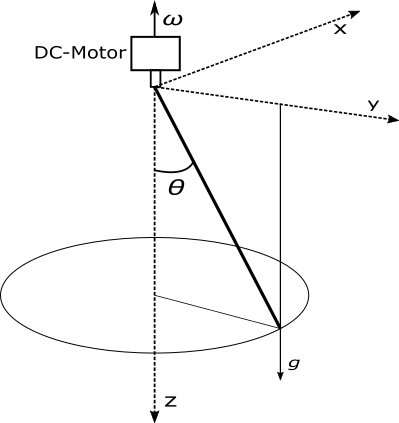
\includegraphics[width=0.5\textwidth,trim={0cm 0cm 4cm 0.45cm},clip]{SkissPendel/g17413.png}
%  }\qquad
%    \end{subfigure}%
%    \hspace{130px}
%    \begin{subfigure}{0.15\textwidth}
%        \centering
%        \subcaptionbox{Dubbel konisk pendel\hspace*{0px}}{%
%    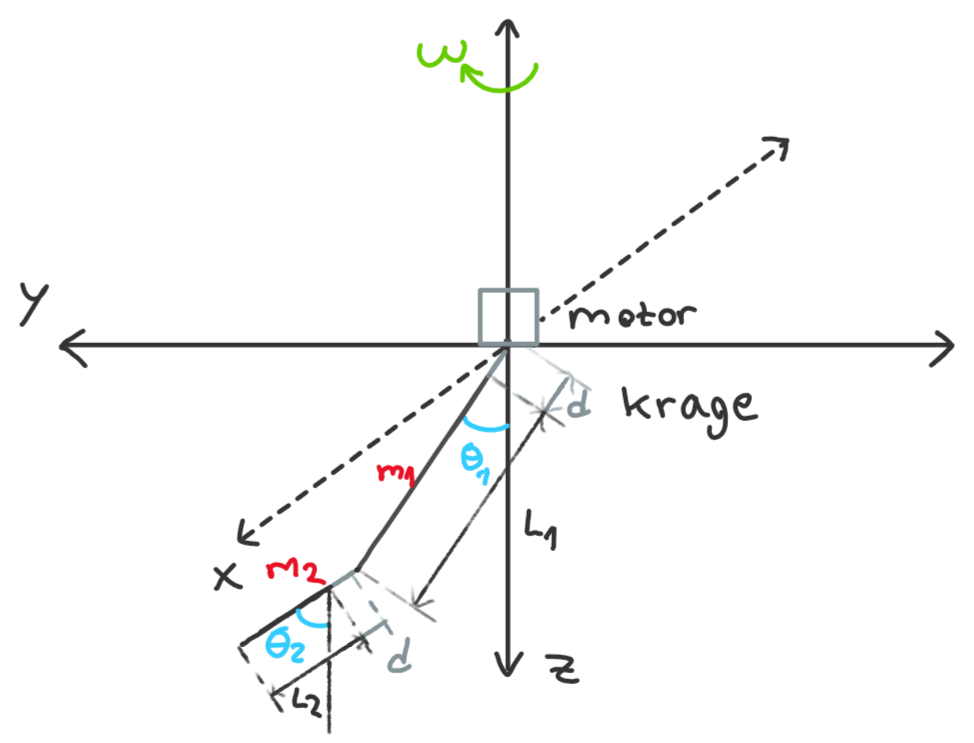
\includegraphics[width=2.5\textwidth,trim={0cm 0cm 4cm 0.45cm},clip]{SkissPendel/extraupg.PNG}
%  }\qquad
%    \end{subfigure}
%    \caption{Schematiska figurer över en enkel konisk pendel och en dubbel konisk pendel. Stång \rom{2} i dubbelpendeln är fäst på %samma sätt som stång \rom{1} med en kardanknut, vilket innebär att den endast kan röra sig i ett plan vinkelrätt mot %rotationsriktningen. }
%    \label{resultat:xuppgf}
%\end{figure}

\begin{figure}[H]
%\hspace{-200px}
    \centering
    \begin{subfigure}[b]{0.45\textwidth}
        \centering
        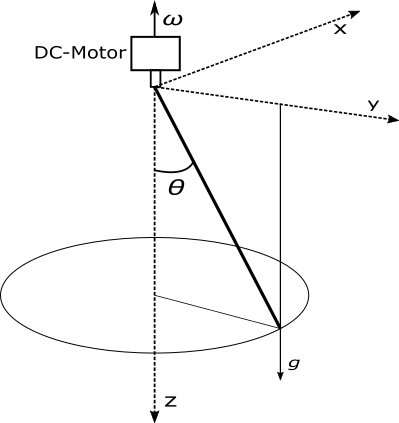
\includegraphics[width=0.8\textwidth]{SkissPendel/g17413.png}
        \caption{Enkel konisk pendel.}
    \end{subfigure}
    \hfill
    \begin{subfigure}[b]{0.45\textwidth}
        \centering
        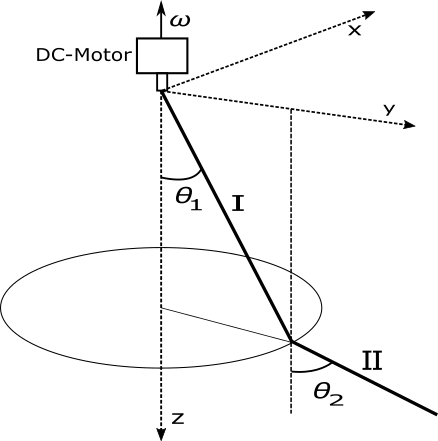
\includegraphics[width=0.85\textwidth]{SkissPendel/text18318-2.png}
        \caption{ Dubbel konisk pendel.}
    \end{subfigure}
    \caption{Schematiska figurer över en enkel konisk pendel och en dubbel konisk pendel.}
    \label{upp:gxuppgf}
\end{figure}

\begin{wrapfigure}[14]{r}{0.20\textwidth}
    \centering
    \vspace{-20px}
    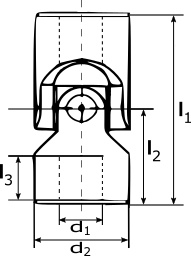
\includegraphics[width = 0.20\textwidth]{gbilder/text6405-4-1-1.png}
    \caption{Profilen för kardanknuten för de koniska pendlarna med längder $l_1 = 48$ mm, $l_2 = 24$ mm, $l_3 = 12$ mm, $d_1 = 10$ mm och $d_2 = 22$ mm.}
    \label{fig:Kardanknut}
\end{wrapfigure}

\subsection{Experimentell uppställning för bestämning av $g$}

En pyramidformad stålram monterades i ett optiskt bord genom att i botten skruvas fast och i toppen spännas fast med spännband fästa i bordet. Ovanpå placerades en DC-motor och en stålstång med längd $L_1 = 205$ mm och massa $m_1 = 128$ g kopplades till DC-motorn med en kardanknut sådan att översta punkten på stången befann sig $d = 12$ mm ifrån kardanknutens vridpunkt. Tillsammans bildade detta system en enkel konisk pendel likt figur \ref{upp:gxuppgf} (a). Vidare placerades två höghastighetskameror av modell Oqus från Qualisys, med förmåga att utföra mätningar på så kallade IR-markörer, under stålramen och riktades mot den koniska pendeln för att uppmäta positionen av den nedre änden av stången. Kamerorna riktades underifrån för att möjliggöra att ändpunkten för stången kontinuerligt var i bild.

Kardanknutens längder anges i figur \ref{fig:Kardanknut} där den undre delen med längd $l_2 = 24$ mm var kopplad till stången och hade en massa $m_k = 35$ g. På grund av att den undre delen i huvudsak består av en ihålig cylinder med längd $l_3 = 12 $ mm modellerades kardanknuten till en ihålig cylinder med längd enligt medelvärdet $l = \frac{l_2 + l_3}{2} = 18$ mm.


\subsection{Experimentell uppställning för analys av dubbel konisk pendel}
För analysen av en dubbel konisk pendel användes samma försöksuppställning som för bestämmandet av $g$. Utöver detta fästes ytterligare en stång med en kardanknut i änden av den övre stången analogt med figur \ref{upp:gxuppgf} (b).

\subsection{Utförande för bestämning av $g$}
En IR-markör fästes på änden av stången för den enkla koniska pendeln sådan att dess position kunde uppmätas av höghastighetskamerorna. Stången roterades av DC-motorn för att bilda vinkeln $\theta$ mot vertikalen varefter positionen på stångens ändpunkt uppmättes med kamerorna under tidsintervall mellan $10-200$ s. Proceduren upprepades för olika $\theta$ vid ett första tillfälle 18 gånger och vid ett andra tillfälle sju gånger.

Utifrån varje mätnings positionsdata beräknades den koniska pendelns vinkelhastighet $\omega$ och vinkel $\theta$ för varje helt roterat varv kring vertikalen, vilket definieras som en period. Vinkelhastigheten bestämdes genom att uppmäta periodtiden för den koniska pendeln. Periodtiden uppmättes genom att finna de lokala maxima för den periodiska positiondatan med hjälp av funktionen \textit{findpeaks} i Matlab. 

Vinkeln $\theta$ beräknades i tre steg vilka bygger på observationen att positionsdatan för en period spänner upp en tredimensionell ellips. Först anpassades ett plan med minstakvadratmetoden till en periods positionsdata. Sedan beräknades basvektorer till planet för att projicera den tredimensionella ellipsen till två dimensioner. Följden blev att tvådimensionell elliptisk minstakvadratmetod kunde appliceras för att anpassa en ellips till positionsdatan. Utifrån den anpassade ellipsen kunde dess axlar beräknas varav vinkeln $\theta$ var möjlig att beräkna enligt sambandet $\sin \theta = \frac{d_e}{2L}$, där $d_e$ är medelvärdet av axlarnas längd. Slutligen beräknades $g$ för varje period enligt ekvation \eqref{eq: g}.

\subsection{Utförande för analys av dubbel konisk pendel}
Den dubbla koniska pendeln analyserades genom försätta systemet i på förhand bestämda initialvillkor för $\theta_1$, $\theta_2$ och $\omega$. Den dubbla koniska pendeln simulerades för dessa initialvillkor med hjälp av ekvationssystem \eqref{eq:dkp} varav den dubbla koniska pendeln sedan analyserades experimentellt. Experimentellt åstadkoms initialvillkoren genom att första fixera vinkelförhållanden mellan stång \rom{1} och stång \rom{2} med en spoltråd. Den ena spoltrådsänden fästes mot motoraxeln och den andra på änden av stång \rom{2}. Med vinklarna fixerade användes DC-motorn för att få systemet att uppnå ett jämviktsläge med de initialvinklar och den rotationshastighet som skulle undersökas. Initialvillkoren bestämdes genom att göra en kortare mätning med höghastighetskamorerna ur vilken initialvillkoren kunde härledas genom att utnyttja uppspända ellipser analogt med bestämningen av $g$. 

Därefter startades en ny mätning och spoltrådsänden fäst mot motoraxeln lossades. Motoraxeln valdes då eventuella krafter genom motoraxeln ej påverkar systemet. Positionen för den undre stångens ändpunkt uppmättes av kamerorna, och den uppmätta datan jämfördes mot systemets simulerade beteende med de initiallvillkor som bestämdes under mätningen med fixerade vinklar. Denna process upprepades för olika rotationshastigheter  $\omega$ och därmed olika initialvillkor för systemet.

\section{Resultat och diskussion}
För att tydliggöra metodiken för uppmätningen av $g$ kommer nedan resultat presenters genom att först i detalj redogöra för resultatet av en mätning, mätning tre, för att sedan presentera det sammanlagda resultatet från alla mätningar. Efteråt presenteras resultatet ifrån simuleringar och mätningar av den dubbla koniska pendeln.

\subsection{Resultat och diskussion för bestämning av $g$}
Positionsdata med anpassat plan för sista perioden i mätning tre presenteras i figur \ref{resultat: matning3} (a). Observera den tredimensionella ellipsen som utnyttjas för att beräkna vinkeln $\theta$ som presenteras med vinkelhastigheten $\omega$ för mätningens alla perioder i figur \ref{resultat: matning3} (b). För sista perioden var ellipsens storaxel $a = 159.8$ mm och lillaxel $b = 159.2$ mm och därmed i hög grad cirkulär.
\newline


\begin{figure}[H]
    \hspace{-40px}
    \centering
    \begin{subfigure}[b]{0.40\textwidth}
        \centering
        \setlength\fheight{1.8in}
        % This file was created by matlab2tikz.
%
%The latest updates can be retrieved from
%  http://www.mathworks.com/matlabcentral/fileexchange/22022-matlab2tikz-matlab2tikz
%where you can also make suggestions and rate matlab2tikz.
%
\definecolor{mycolor1}{rgb}{0.00000,0.44700,0.74100}%
\definecolor{mycolor2}{rgb}{0.178, 0.70,0}%
%
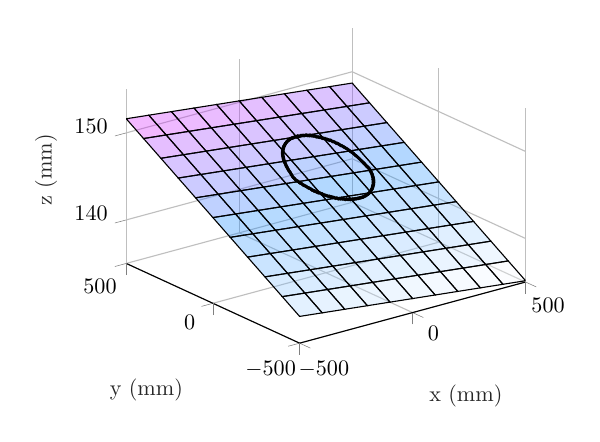
\begin{tikzpicture}[scale = 1.0, every node/.style={scale = 0.80}, domain = 0:2]

\begin{axis}[%
width=1.268\fheight,
height=\fheight,
at={(0\fheight,0\fheight)},
scale only axis,
xmin=-500,
xmax=500,
tick align=outside,
ymin=-500,
ymax=500,
zmin=135,
zmax=155,
view={-37.5}{30},
axis background/.style={fill=white},
axis x line*=bottom,
axis y line*=left,
axis z line*=left,
xmajorgrids,
ymajorgrids,
zmajorgrids,
xlabel style={font=\color{white!15!black}},
xlabel={x (\text{mm})},
ylabel style={font=\color{white!15!black}},
ylabel={y (\text{mm})},
zlabel style={font=\color{white!15!black}},
zlabel={z (\text{mm})}
]
\addplot3[only marks, mark=o, mark options={}, mark size=0.4pt, draw=black, opacity=1.25] table[row sep=crcr]{%
x	y	z\\
276.494	137.822	144.294\\
276.485	140.968	144.367\\
276.457	144.106	144.356\\
276.328	147.318	144.429\\
276.156	150.447	144.468\\
275.927	153.633	144.513\\
275.618	156.816	144.522\\
275.233	159.973	144.588\\
274.813	163.13	144.626\\
274.331	166.202	144.685\\
273.788	169.331	144.723\\
273.169	172.474	144.774\\
272.508	175.57	144.839\\
271.778	178.656	144.895\\
270.982	181.739	144.895\\
270.125	184.804	144.941\\
269.189	187.822	145\\
268.213	190.852	145.09\\
267.16	193.866	145.103\\
266.077	196.846	145.159\\
264.912	199.784	145.189\\
263.701	202.735	145.251\\
262.421	205.648	145.287\\
261.086	208.542	145.368\\
259.677	211.396	145.404\\
258.216	214.198	145.46\\
256.724	217.003	145.487\\
255.167	219.777	145.537\\
253.56	222.531	145.572\\
251.893	225.232	145.625\\
250.163	227.91	145.673\\
248.362	230.542	145.73\\
246.52	233.123	145.738\\
244.631	235.693	145.76\\
242.688	238.224	145.839\\
240.695	240.747	145.895\\
238.651	243.166	145.948\\
236.552	245.564	145.955\\
234.426	247.927	145.981\\
232.227	250.262	146.064\\
229.986	252.538	146.103\\
227.695	254.805	146.135\\
225.371	256.957	146.149\\
222.999	259.085	146.241\\
220.585	261.176	146.281\\
218.123	263.263	146.276\\
215.614	265.233	146.309\\
213.085	267.215	146.348\\
210.498	269.061	146.399\\
207.893	270.898	146.414\\
205.23	272.712	146.486\\
202.555	274.423	146.487\\
199.848	276.133	146.512\\
197.077	277.71	146.527\\
194.299	279.309	146.58\\
191.457	280.839	146.637\\
188.609	282.257	146.651\\
185.711	283.684	146.679\\
182.798	285.003	146.713\\
179.88	286.29	146.72\\
176.924	287.534	146.747\\
173.933	288.68	146.819\\
170.911	289.772	146.87\\
167.871	290.802	146.867\\
164.836	291.795	146.914\\
161.757	292.685	146.927\\
158.658	293.533	146.939\\
155.538	294.346	147.03\\
152.433	295.078	146.964\\
149.295	295.788	147.02\\
146.16	296.336	147.034\\
143.008	296.908	147.064\\
139.81	297.371	147.116\\
136.636	297.781	147.104\\
133.437	298.109	147.09\\
130.249	298.408	147.118\\
127.061	298.665	147.144\\
123.878	298.833	147.156\\
120.657	298.994	147.157\\
117.452	299.001	147.194\\
114.258	298.91	147.138\\
111.046	298.828	147.162\\
107.863	298.643	147.198\\
104.655	298.478	147.219\\
101.477	298.176	147.263\\
98.277	297.814	147.184\\
95.11	297.453	147.241\\
91.939	296.941	147.23\\
88.788	296.399	147.26\\
85.64	295.824	147.213\\
82.505	295.182	147.237\\
79.391	294.385	147.231\\
76.285	293.634	147.257\\
73.177	292.8	147.281\\
70.111	291.87	147.263\\
67.087	290.921	147.259\\
64.049	289.883	147.224\\
61.017	288.781	147.243\\
58.032	287.587	147.249\\
55.065	286.399	147.2\\
52.123	285.144	147.205\\
49.235	283.823	147.194\\
46.353	282.414	147.222\\
43.481	280.943	147.217\\
40.651	279.507	147.166\\
37.859	277.958	147.157\\
35.108	276.366	147.131\\
32.362	274.654	147.119\\
29.679	272.923	147.125\\
26.986	271.148	147.065\\
24.357	269.339	147.069\\
21.781	267.432	147.035\\
19.212	265.497	147.028\\
16.691	263.501	147.002\\
14.208	261.478	147.002\\
11.765	259.417	146.932\\
9.392	257.227	146.935\\
7.018	255.076	146.913\\
4.727	252.825	146.923\\
2.456	250.581	146.863\\
0.237	248.236	146.855\\
-1.93	245.887	146.785\\
-4.05	243.452	146.771\\
-6.142	241.028	146.718\\
-8.157	238.535	146.696\\
-10.116	235.988	146.67\\
-12.045	233.412	146.637\\
-13.917	230.811	146.615\\
-15.735	228.14	146.57\\
-17.491	225.477	146.504\\
-19.187	222.792	146.48\\
-20.835	220.031	146.442\\
-22.43	217.255	146.437\\
-23.973	214.47	146.373\\
-25.464	211.623	146.336\\
-26.886	208.726	146.299\\
-28.244	205.865	146.267\\
-29.559	202.942	146.225\\
-30.804	200.013	146.181\\
-31.989	196.999	146.115\\
-33.108	193.985	146.154\\
-34.179	190.981	146.089\\
-35.202	187.945	146.059\\
-36.152	184.85	146.002\\
-37.029	181.819	145.896\\
-37.86	178.715	145.895\\
-38.622	175.572	145.815\\
-39.306	172.454	145.823\\
-39.966	169.337	145.738\\
-40.553	166.205	145.7\\
-41.066	163.048	145.63\\
-41.507	159.874	145.579\\
-41.892	156.701	145.52\\
-42.204	153.503	145.506\\
-42.453	150.323	145.401\\
-42.614	147.17	145.356\\
-42.721	143.987	145.282\\
-42.776	140.804	145.217\\
-42.767	137.651	145.147\\
-42.678	134.44	145.055\\
-42.529	131.292	144.996\\
-42.342	128.167	145.007\\
-42.067	124.942	144.935\\
-41.746	121.773	144.887\\
-41.346	118.591	144.792\\
-40.904	115.455	144.814\\
-40.402	112.309	144.799\\
-39.811	109.163	144.794\\
-39.18	106.018	144.732\\
-38.516	102.891	144.692\\
-37.725	99.788	144.653\\
-36.885	96.747	144.663\\
-36.01	93.675	144.645\\
-35.037	90.584	144.587\\
-34.039	87.607	144.526\\
-32.969	84.584	144.499\\
-31.827	81.592	144.502\\
-30.653	78.623	144.439\\
-29.38	75.722	144.433\\
-28.066	72.801	144.388\\
-26.727	69.882	144.333\\
-25.292	67.093	144.306\\
-23.794	64.233	144.288\\
-22.274	61.429	144.24\\
-20.669	58.697	144.227\\
-19.014	55.982	144.12\\
-17.32	53.264	144.141\\
-15.565	50.615	144.047\\
-13.728	47.972	144.053\\
-11.862	45.418	144.028\\
-9.949	42.848	143.954\\
-7.963	40.388	143.959\\
-5.932	37.886	143.895\\
-3.861	35.447	143.874\\
-1.744	33.08	143.884\\
0.416	30.695	143.817\\
2.636	28.406	143.79\\
4.906	26.151	143.783\\
7.227	23.911	143.698\\
9.582	21.747	143.671\\
11.992	19.642	143.637\\
14.433	17.562	143.596\\
16.9	15.506	143.587\\
19.427	13.57	143.538\\
22.004	11.674	143.518\\
24.613	9.752	143.511\\
27.243	7.951	143.446\\
29.938	6.201	143.447\\
32.637	4.505	143.392\\
35.393	2.807	143.376\\
38.16	1.237	143.345\\
40.975	-0.331	143.279\\
43.837	-1.807	143.283\\
46.692	-3.207	143.293\\
49.611	-4.614	143.194\\
52.533	-5.89	143.19\\
55.48	-7.175	143.197\\
58.457	-8.345	143.15\\
61.473	-9.467	143.184\\
64.505	-10.537	143.113\\
67.552	-11.566	143.133\\
70.609	-12.523	143.092\\
73.698	-13.43	143.048\\
76.806	-14.271	143.016\\
79.965	-15.02	143.052\\
83.068	-15.709	142.991\\
86.226	-16.405	142.987\\
89.38	-16.913	142.948\\
92.571	-17.485	142.942\\
95.751	-17.901	142.886\\
98.919	-18.298	142.894\\
102.119	-18.63	142.914\\
105.313	-18.9	142.882\\
108.521	-19.105	142.882\\
111.73	-19.202	142.863\\
114.94	-19.29	142.853\\
118.157	-19.314	142.854\\
121.351	-19.258	142.822\\
124.547	-19.1	142.845\\
127.775	-18.913	142.819\\
130.967	-18.677	142.808\\
134.161	-18.351	142.817\\
137.344	-18.004	142.787\\
140.505	-17.528	142.802\\
143.685	-17.049	142.779\\
146.849	-16.455	142.784\\
150.003	-15.818	142.777\\
153.121	-15.122	142.757\\
156.241	-14.376	142.77\\
159.35	-13.565	142.778\\
162.432	-12.645	142.788\\
165.491	-11.705	142.779\\
168.533	-10.713	142.767\\
171.553	-9.64	142.769\\
174.561	-8.508	142.796\\
177.53	-7.308	142.8\\
180.513	-6.072	142.804\\
183.442	-4.789	142.807\\
186.338	-3.399	142.804\\
189.198	-1.992	142.803\\
192.028	-0.522	142.837\\
194.874	1.05	142.867\\
197.654	2.642	142.88\\
200.4	4.272	142.876\\
203.102	5.948	142.909\\
205.798	7.755	142.93\\
208.449	9.541	142.973\\
211.054	11.416	142.998\\
213.646	13.325	142.96\\
216.185	15.307	143.034\\
218.7	17.326	143.009\\
221.172	19.393	143.024\\
223.543	21.5	143.089\\
225.912	23.654	143.13\\
228.261	25.901	143.145\\
230.548	28.148	143.157\\
232.774	30.458	143.191\\
234.94	32.785	143.203\\
237.108	35.198	143.229\\
239.201	37.625	143.289\\
241.249	40.125	143.298\\
243.228	42.615	143.325\\
245.165	45.142	143.358\\
247.046	47.755	143.416\\
248.878	50.334	143.445\\
250.652	53.008	143.463\\
252.384	55.696	143.469\\
254.063	58.433	143.541\\
255.667	61.19	143.537\\
257.237	63.979	143.579\\
258.733	66.81	143.621\\
260.201	69.68	143.636\\
261.56	72.536	143.678\\
262.883	75.434	143.722\\
264.168	78.343	143.765\\
265.363	81.293	143.782\\
266.525	84.284	143.819\\
267.593	87.243	143.847\\
268.63	90.313	143.897\\
269.589	93.343	143.901\\
270.502	96.397	143.926\\
271.343	99.494	143.991\\
272.117	102.567	144.019\\
272.826	105.659	144.077\\
273.508	108.75	144.08\\
274.079	111.88	144.059\\
274.629	115.026	144.134\\
275.095	118.194	144.165\\
275.512	121.33	144.159\\
275.843	124.48	144.137\\
276.113	127.662	144.155\\
276.313	130.853	144.252\\
276.455	134.016	144.283\\
276.54	137.15	144.285\\
276.555	140.312	144.31\\
};

\addplot3[%
surf,
fill opacity=0.3, shader=flat corner, draw=black, z buffer=sort, colormap={mymap}{[1pt] rgb(0pt)=(0.2422,0.1504,0.6603); rgb(1pt)=(0.25039,0.164995,0.707614); rgb(2pt)=(0.257771,0.181781,0.751138); rgb(3pt)=(0.264729,0.197757,0.795214); rgb(4pt)=(0.270648,0.214676,0.836371); rgb(5pt)=(0.275114,0.234238,0.870986); rgb(6pt)=(0.2783,0.255871,0.899071); rgb(7pt)=(0.280333,0.278233,0.9221); rgb(8pt)=(0.281338,0.300595,0.941376); rgb(9pt)=(0.281014,0.322757,0.957886); rgb(10pt)=(0.279467,0.344671,0.971676); rgb(11pt)=(0.275971,0.366681,0.982905); rgb(12pt)=(0.269914,0.3892,0.9906); rgb(13pt)=(0.260243,0.412329,0.995157); rgb(14pt)=(0.244033,0.435833,0.998833); rgb(15pt)=(0.220643,0.460257,0.997286); rgb(16pt)=(0.196333,0.484719,0.989152); rgb(17pt)=(0.183405,0.507371,0.979795); rgb(18pt)=(0.178643,0.528857,0.968157); rgb(19pt)=(0.176438,0.549905,0.952019); rgb(20pt)=(0.168743,0.570262,0.935871); rgb(21pt)=(0.154,0.5902,0.9218); rgb(22pt)=(0.146029,0.609119,0.907857); rgb(23pt)=(0.138024,0.627629,0.89729); rgb(24pt)=(0.124814,0.645929,0.888343); rgb(25pt)=(0.111252,0.6635,0.876314); rgb(26pt)=(0.0952095,0.679829,0.859781); rgb(27pt)=(0.0688714,0.694771,0.839357); rgb(28pt)=(0.0296667,0.708167,0.816333); rgb(29pt)=(0.00357143,0.720267,0.7917); rgb(30pt)=(0.00665714,0.731214,0.766014); rgb(31pt)=(0.0433286,0.741095,0.73941); rgb(32pt)=(0.0963952,0.75,0.712038); rgb(33pt)=(0.140771,0.7584,0.684157); rgb(34pt)=(0.1717,0.766962,0.655443); rgb(35pt)=(0.193767,0.775767,0.6251); rgb(36pt)=(0.216086,0.7843,0.5923); rgb(37pt)=(0.246957,0.791795,0.556743); rgb(38pt)=(0.290614,0.79729,0.518829); rgb(39pt)=(0.340643,0.8008,0.478857); rgb(40pt)=(0.3909,0.802871,0.435448); rgb(41pt)=(0.445629,0.802419,0.390919); rgb(42pt)=(0.5044,0.7993,0.348); rgb(43pt)=(0.561562,0.794233,0.304481); rgb(44pt)=(0.617395,0.787619,0.261238); rgb(45pt)=(0.671986,0.779271,0.2227); rgb(46pt)=(0.7242,0.769843,0.191029); rgb(47pt)=(0.773833,0.759805,0.16461); rgb(48pt)=(0.820314,0.749814,0.153529); rgb(49pt)=(0.863433,0.7406,0.159633); rgb(50pt)=(0.903543,0.733029,0.177414); rgb(51pt)=(0.939257,0.728786,0.209957); rgb(52pt)=(0.972757,0.729771,0.239443); rgb(53pt)=(0.995648,0.743371,0.237148); rgb(54pt)=(0.996986,0.765857,0.219943); rgb(55pt)=(0.995205,0.789252,0.202762); rgb(56pt)=(0.9892,0.813567,0.188533); rgb(57pt)=(0.978629,0.838629,0.176557); rgb(58pt)=(0.967648,0.8639,0.16429); rgb(59pt)=(0.96101,0.889019,0.153676); rgb(60pt)=(0.959671,0.913457,0.142257); rgb(61pt)=(0.962795,0.937338,0.12651); rgb(62pt)=(0.969114,0.960629,0.106362); rgb(63pt)=(0.9769,0.9839,0.0805)}, 
colormap={cool}{rgb255(0cm)=(255,255,255); rgb255(1cm)=(0,128,255); rgb255(2cm)=(255,0,255)},
mesh/rows=11]
table[row sep=crcr, point meta=\thisrow{c}] {%
%
x	y	z	c\\
-500	-500	138.07301048206	138.07301048206\\
-500	-400	139.427996975828	139.427996975828\\
-500	-300	140.782983469596	140.782983469596\\
-500	-200	142.137969963365	142.137969963365\\
-500	-100	143.492956457133	143.492956457133\\
-500	0	144.847942950902	144.847942950902\\
-500	100	146.20292944467	146.20292944467\\
-500	200	147.557915938438	147.557915938438\\
-500	300	148.912902432207	148.912902432207\\
-500	400	150.267888925975	150.267888925975\\
-500	500	151.622875419743	151.622875419743\\
-400	-500	137.780704281504	137.780704281504\\
-400	-400	139.135690775272	139.135690775272\\
-400	-300	140.49067726904	140.49067726904\\
-400	-200	141.845663762809	141.845663762809\\
-400	-100	143.200650256577	143.200650256577\\
-400	0	144.555636750345	144.555636750345\\
-400	100	145.910623244114	145.910623244114\\
-400	200	147.265609737882	147.265609737882\\
-400	300	148.620596231651	148.620596231651\\
-400	400	149.975582725419	149.975582725419\\
-400	500	151.330569219187	151.330569219187\\
-300	-500	137.488398080947	137.488398080947\\
-300	-400	138.843384574716	138.843384574716\\
-300	-300	140.198371068484	140.198371068484\\
-300	-200	141.553357562253	141.553357562253\\
-300	-100	142.908344056021	142.908344056021\\
-300	0	144.263330549789	144.263330549789\\
-300	100	145.618317043558	145.618317043558\\
-300	200	146.973303537326	146.973303537326\\
-300	300	148.328290031094	148.328290031094\\
-300	400	149.683276524863	149.683276524863\\
-300	500	151.038263018631	151.038263018631\\
-200	-500	137.196091880391	137.196091880391\\
-200	-400	138.55107837416	138.55107837416\\
-200	-300	139.906064867928	139.906064867928\\
-200	-200	141.261051361696	141.261051361696\\
-200	-100	142.616037855465	142.616037855465\\
-200	0	143.971024349233	143.971024349233\\
-200	100	145.326010843001	145.326010843001\\
-200	200	146.68099733677	146.68099733677\\
-200	300	148.035983830538	148.035983830538\\
-200	400	149.390970324307	149.390970324307\\
-200	500	150.745956818075	150.745956818075\\
-100	-500	136.903785679835	136.903785679835\\
-100	-400	138.258772173603	138.258772173603\\
-100	-300	139.613758667372	139.613758667372\\
-100	-200	140.96874516114	140.96874516114\\
-100	-100	142.323731654909	142.323731654909\\
-100	0	143.678718148677	143.678718148677\\
-100	100	145.033704642445	145.033704642445\\
-100	200	146.388691136214	146.388691136214\\
-100	300	147.743677629982	147.743677629982\\
-100	400	149.09866412375	149.09866412375\\
-100	500	150.453650617519	150.453650617519\\
0	-500	136.611479479279	136.611479479279\\
0	-400	137.966465973047	137.966465973047\\
0	-300	139.321452466816	139.321452466816\\
0	-200	140.676438960584	140.676438960584\\
0	-100	142.031425454352	142.031425454352\\
0	0	143.386411948121	143.386411948121\\
0	100	144.741398441889	144.741398441889\\
0	200	146.096384935658	146.096384935658\\
0	300	147.451371429426	147.451371429426\\
0	400	148.806357923194	148.806357923194\\
0	500	150.161344416963	150.161344416963\\
100	-500	136.319173278723	136.319173278723\\
100	-400	137.674159772491	137.674159772491\\
100	-300	139.02914626626	139.02914626626\\
100	-200	140.384132760028	140.384132760028\\
100	-100	141.739119253796	141.739119253796\\
100	0	143.094105747565	143.094105747565\\
100	100	144.449092241333	144.449092241333\\
100	200	145.804078735101	145.804078735101\\
100	300	147.15906522887	147.15906522887\\
100	400	148.514051722638	148.514051722638\\
100	500	149.869038216406	149.869038216406\\
200	-500	136.026867078167	136.026867078167\\
200	-400	137.381853571935	137.381853571935\\
200	-300	138.736840065703	138.736840065703\\
200	-200	140.091826559472	140.091826559472\\
200	-100	141.44681305324	141.44681305324\\
200	0	142.801799547009	142.801799547009\\
200	100	144.156786040777	144.156786040777\\
200	200	145.511772534545	145.511772534545\\
200	300	146.866759028314	146.866759028314\\
200	400	148.221745522082	148.221745522082\\
200	500	149.57673201585	149.57673201585\\
300	-500	135.734560877611	135.734560877611\\
300	-400	137.089547371379	137.089547371379\\
300	-300	138.444533865147	138.444533865147\\
300	-200	139.799520358916	139.799520358916\\
300	-100	141.154506852684	141.154506852684\\
300	0	142.509493346452	142.509493346452\\
300	100	143.864479840221	143.864479840221\\
300	200	145.219466333989	145.219466333989\\
300	300	146.574452827757	146.574452827757\\
300	400	147.929439321526	147.929439321526\\
300	500	149.284425815294	149.284425815294\\
400	-500	135.442254677054	135.442254677054\\
400	-400	136.797241170823	136.797241170823\\
400	-300	138.152227664591	138.152227664591\\
400	-200	139.507214158359	139.507214158359\\
400	-100	140.862200652128	140.862200652128\\
400	0	142.217187145896	142.217187145896\\
400	100	143.572173639665	143.572173639665\\
400	200	144.927160133433	144.927160133433\\
400	300	146.282146627201	146.282146627201\\
400	400	147.63713312097	147.63713312097\\
400	500	148.992119614738	148.992119614738\\
500	-500	135.149948476498	135.149948476498\\
500	-400	136.504934970267	136.504934970267\\
500	-300	137.859921464035	137.859921464035\\
500	-200	139.214907957803	139.214907957803\\
500	-100	140.569894451572	140.569894451572\\
500	0	141.92488094534	141.92488094534\\
500	100	143.279867439108	143.279867439108\\
500	200	144.634853932877	144.634853932877\\
500	300	145.989840426645	145.989840426645\\
500	400	147.344826920414	147.344826920414\\
500	500	148.699813414182	148.699813414182\\
};
\end{axis}
\end{tikzpicture}%
        \caption{Positionsdata för sista perioden för mätning tre (svarta markeringar som bildar en ellips) med anpassat plan med minsta kvadratmetoden.}
    \end{subfigure}
    \hspace{30px}
    \begin{subfigure}[b]{0.45\textwidth}
        \centering
        \setlength\fheight{1.7in}
        % This file was created by matlab2tikz.
%
%The latest updates can be retrieved from
%  http://www.mathworks.com/matlabcentral/fileexchange/22022-matlab2tikz-matlab2tikz
%where you can also make suggestions and rate matlab2tikz.
\definecolor{mycolor1}{rgb}{0.00000,0.44700,0.74100}
%
\begin{tikzpicture}[scale = 1.0, every node/.style={scale = 0.80}, domain = 0:2]

\begin{axis}[%
width=1.25\fheight,
height=\fheight,
at={(0\fheight,0\fheight)},
scale only axis,
%y axis line style={blue, ultra thick},
xmin=0,
xmax=15.5,
%xlabel style={font=\color{white!15!black}},
xlabel={\text{Period}},
axis y line*=left,
ymin=10.00,
ymax=10.075,
ylabel style={font=\color{white!15!black}},
ylabel={$\omega$ (\text{rad/s})},
ytick = {10.01, 10.04, 10.07},
yticklabels = {10.01, 10.04, 10.07},
%axis background/.style={fill=white},
%legend style={legend cell align=left, align=left, draw=white!15!black}
]
\addplot [only marks, mark size = 2pt, mark=square, color=mycolor1, opacity=1.25]
  table[row sep=crcr]{%
1	10.0050721451904\\
2	10.0370372319163\\
3	10.0370372319163\\
4	10.0370372319163\\
5	10.0370372319163\\
6	10.0692072230442\\
7	10.0692072230442\\
8	10.0692072230442\\
9	10.0692072230442\\
10	10.0692072230442\\
11	10.0692072230442\\
12	10.0692072230442\\
13	10.0370372319163\\
14	10.0370372319163\\
15	10.0370372319163\\
}; \label{plot_one}

% \addlegendentry{Vinkelhastighet $\omega$}
\end{axis}
%
\begin{axis}[%
width=1.25\fheight,
height=\fheight,
at={(0\fheight,0\fheight)},
scale only axis,
xmin=0,
xmax=15.5,
axis y line*=right,
ymin= 0.805,
ymax= 0.8155,
ylabel style={font=\color{white!15!black}},
ylabel={$\theta$ (\text{rad})},
x axis line style = {opacity = 0},
%y axis line style={black, ultra thick},
ytick = {0.806, 0.810, 0.815},
yticklabels = {0.806, 0.810, 0.815},
xticklabels = { , , , },
%legend pos = north west,
legend style={at={(0.55, 0.22)},anchor=north}
]
\addlegendimage{/pgfplots/refstyle=plot_one}\addlegendentry{Vinkelhastighet $\omega$}
\addplot [only marks, mark size = 3pt, mark=triangle, color=black, opacity=1.25]
  table[row sep=crcr]{%
1	0.805859336610269\\
2	0.805701942847216\\
3	0.80591635811605\\
4	0.808057385095893\\
5	0.810111385067792\\
6	0.811215250116312\\
7	0.812263931424508\\
8	0.8131598234478\\
9	0.813473495970097\\
10	0.813415540967618\\
11	0.812815370658134\\
12	0.811336415273185\\
13	0.809233237903385\\
14	0.806680211635308\\
15	0.806492634658544\\
}; 
\addlegendentry{Vinkel $\theta$}

\end{axis}
\end{tikzpicture}%
%legend style={at={(0.27,0.45)}, anchor = north, nodes={scale=0.80, transform shape}
        \caption{Vinkelhastigheten $\omega$ som funktion av antal varv (blå kvadrater) och vinkeln $\theta$ som funktion av antal perioder (svarta trianglar).}
    \end{subfigure}
    \caption{Uppmätta och beräknade storheter från mätning tre.} 
    \label{resultat: matning3}
\end{figure}

Det första vi observerar i figur \ref{resultat: matning3} (a) är att ellipsen och det anpassade planet inte är parallellt med det horisontella xy-planet. Detta medför att motoraxeln ej var parallell mot vertikalen. Konsekvensen blir att teoridelens antagande om att motoraxeln är parallell med vertikalen inte uppfylls. 

Dupré och Janssen observerade även i sina mätningar att motoraxeln var vinklad mot vertikalen. I deras artikel uppskattar de motoraxelns vinkel mot vertikalen till $\theta_0 = 0.0035^\text{o}$ under antagandet att International Gravity Formula \cite{gravformula} är korrekt. Till skillnad från deras arbete är det möjligt utifrån studiens mätningar att uppskatta motoraxelns vinkel utan ovan antagande. Det anpassade planet för mätning tre har vinkel $\cos \alpha = \frac{\hat{z} \cdot \hat{n}}{\lVert z \rVert \lVert n \rVert} \implies \alpha \approx 0.8^\text{o}$ mot xy-planet. Då följer av uppställningens geometri att motorvinkeln är $\theta_0 \approx 0.3^\text{o}$. Alltså är motorvinkeln liten men dess effekter observerbara.

Vidare observeras i figur \ref{resultat: matning3} (b) att $\omega$ och $\theta$ varierar som funktioner av period inom ett intervall av $\pm 0.5 \%$. Variationerna implicerar att det andra antagandet i teoridelen, att $\omega$ och $\theta$ är konstanta, ej är uppfyllt. Att $\omega$ och $\theta$ varierar observeras även i de andra mätningarna. Däremot, likt den lilla motoraxelvinkeln, är dessa variationer små och i storleksordning av $1\%$. 

Fortsättningsvis utfördes sammanlagt 25 mätserier vilket resulterade i 2547 perioder och därmed 2547 mätningar av $g$. Analogt med ovan tillvägagångssätt för mätning tre uppmättes  $\omega$ och $\theta$ för varje period varav $g$ beräknades enligt ekvation \eqref{eq: g}. Resultatet för $g$ som funktion av period visas i figur \ref{fig: gTotal}.


\begin{figure}[H]
    \centering
    \setlength\fheight{2in}
    % This file was created by matlab2tikz.
%
%The latest updates can be retrieved from
%  http://www.mathworks.com/matlabcentral/fileexchange/22022-matlab2tikz-matlab2tikz
%where you can also make suggestions and rate matlab2tikz.
%
\definecolor{mycolor1}{rgb}{0.00000,0.44700,0.74100}%
%
\begin{tikzpicture}[scale = 1.0, every node/.style={scale = .90}, domain = 0:2]

\begin{axis}[%
width=1.616\fheight,
height=\fheight,
at={(0\fheight,0\fheight)},
scale only axis,
xmin=0,
xmax=3000,
xtick={0, 1000, 2000, 3000},
xticklabels={0, 1000, 2000, 3000},
xlabel style={font=\color{white!15!black}},
xlabel={$\text{Period}$},
ymin=9.5,
ymax=10,
ytick={9.50, 9.60, 9.70, 9.80, 9.90, 10},
yticklabels={9.50, 9.60, 9.70, 9.80, 9.90, 10},
ylabel style={font=\color{white!15!black}},
ylabel={$g$ ($\text{m}/\text{s}^2$)},
axis background/.style={fill=white}
]
\addplot [color=mycolor1, draw=none, mark=o, mark size = 0.75pt, mark options={solid, mycolor1}, forget plot, opacity = 0.75]
  table[row sep=crcr]{%
1	9.8130299999998\\
2	9.84308999999985\\
3	9.80040000000008\\
4	9.81584999999995\\
5	9.77062999999998\\
6	9.7797099999998\\
7	9.7817\\
8	9.83905999999979\\
9	9.7782900000002\\
10	9.82646000000022\\
11	9.80632999999989\\
12	9.79502000000002\\
13	9.7803100000001\\
14	9.82531000000017\\
15	9.78686000000016\\
16	9.78843000000006\\
17	9.78963999999996\\
18	9.79025000000001\\
19	9.79973999999993\\
20	9.80637999999999\\
21	9.81827000000021\\
22	9.74875999999995\\
23	9.81271000000015\\
24	9.76537000000008\\
25	9.84216000000015\\
26	9.74809000000005\\
27	9.84884000000011\\
28	9.76715000000013\\
29	9.85449999999992\\
30	9.74024999999983\\
31	9.80418999999984\\
32	9.80200000000013\\
33	9.7801199999999\\
34	9.75907999999981\\
35	9.81034\\
36	9.79950000000008\\
37	9.79023000000007\\
38	9.78697999999986\\
39	9.78758000000016\\
40	9.79379000000017\\
41	9.80907999999999\\
42	9.76807999999983\\
43	9.79419999999982\\
44	9.79611999999997\\
45	9.88671999999997\\
46	9.89228999999978\\
47	9.91816000000017\\
48	9.88050000000021\\
49	9.9042199999999\\
50	9.92840999999999\\
51	9.9083099999998\\
52	9.88119999999981\\
53	9.91060000000016\\
54	9.87739999999985\\
55	9.94374999999991\\
56	9.87363000000005\\
57	9.91726999999992\\
58	9.89100000000008\\
59	9.86841999999979\\
60	9.96612999999979\\
61	9.88574000000017\\
62	9.87606000000005\\
63	9.92522999999983\\
64	9.91701000000012\\
65	9.88212999999996\\
66	9.92633999999998\\
67	9.91987000000017\\
68	9.85593999999992\\
69	9.90756999999985\\
70	9.9090299999998\\
71	9.91244000000006\\
72	9.9045500000002\\
73	9.88693000000012\\
74	9.94293999999991\\
75	9.89028000000008\\
76	9.88398999999981\\
77	9.93262999999979\\
78	9.91111000000001\\
79	9.88378999999986\\
80	9.92349999999988\\
81	9.91440999999986\\
82	9.8453199999999\\
83	9.94194000000016\\
84	9.92133000000013\\
85	9.8452400000001\\
86	9.95577000000003\\
87	9.8399800000002\\
88	9.91681000000017\\
89	9.8751400000001\\
90	9.95281999999997\\
91	9.89777000000004\\
92	9.90877\\
93	9.85685000000012\\
94	9.93870000000015\\
95	9.84130999999979\\
96	9.93906000000015\\
97	9.89798000000019\\
98	9.94234000000006\\
99	9.86254000000008\\
100	9.95438000000013\\
101	9.87021999999979\\
102	9.91127999999981\\
103	9.9095699999998\\
104	9.91170999999986\\
105	9.91222999999991\\
106	9.86572999999999\\
107	9.83393999999998\\
108	9.98741999999993\\
109	9.83849999999984\\
110	9.90659000000005\\
111	9.9062600000002\\
112	9.90389999999979\\
113	9.90963999999985\\
114	9.9025200000001\\
115	9.90135000000009\\
116	9.91145999999981\\
117	9.91908999999987\\
118	9.86153000000013\\
119	9.92047000000002\\
120	9.92871000000014\\
121	9.85548999999992\\
122	9.90122000000019\\
123	9.89766999999983\\
124	9.96007000000009\\
125	9.89611999999988\\
126	9.9043700000002\\
127	9.85066999999981\\
128	9.93353999999999\\
129	9.92833999999993\\
130	9.85188999999991\\
131	9.8727100000001\\
132	9.98610000000008\\
133	9.8724400000001\\
134	9.9342200000001\\
135	9.89134000000013\\
136	9.85417000000007\\
137	9.96093999999994\\
138	9.89953000000014\\
139	9.89604999999983\\
140	9.90281999999979\\
141	9.86790000000019\\
142	9.88599000000022\\
143	9.94489999999996\\
144	9.88707000000022\\
145	9.89251999999988\\
146	9.89496000000008\\
147	9.91318000000001\\
148	9.88756000000012\\
149	9.92696999999998\\
150	9.84789000000001\\
151	9.94885999999997\\
152	9.91512000000012\\
153	9.86220999999978\\
154	9.90250999999989\\
155	9.93391999999994\\
156	9.90693999999985\\
157	9.94016000000011\\
158	9.86580999999978\\
159	9.91818000000012\\
160	9.85363000000007\\
161	9.89897000000019\\
162	9.93805999999995\\
163	9.86346999999978\\
164	9.93256999999994\\
165	9.87577999999985\\
166	9.93357999999989\\
167	9.91354000000001\\
168	9.88997999999992\\
169	9.92052999999987\\
170	9.89636000000019\\
171	9.8767600000001\\
172	9.93082999999979\\
173	9.88382000000001\\
174	9.88770000000022\\
175	9.89323000000013\\
176	9.91289000000006\\
177	9.88142999999991\\
178	9.91388999999981\\
179	9.88783000000012\\
180	9.95272999999997\\
181	9.88814000000002\\
182	9.88482000000022\\
183	9.8733699999998\\
184	9.97631000000001\\
185	9.83991000000015\\
186	9.89141999999993\\
187	9.94734999999991\\
188	9.86574999999993\\
189	9.91508000000022\\
190	9.89879000000019\\
191	9.94052999999985\\
192	9.92293000000018\\
193	9.83041000000003\\
194	9.92061999999987\\
195	9.89375999999993\\
196	9.93409999999994\\
197	9.92155000000002\\
198	9.85480000000007\\
199	9.91312999999991\\
200	9.86346999999978\\
201	9.93843000000015\\
202	9.95200000000023\\
203	9.83843999999999\\
204	9.89323999999988\\
205	9.90846999999985\\
206	9.91901999999982\\
207	9.8739300000002\\
208	9.86961999999994\\
209	9.92385999999988\\
210	9.87402999999995\\
211	9.95155999999997\\
212	9.86859999999979\\
213	9.89926000000014\\
214	9.9037400000002\\
215	9.94394000000011\\
216	9.8456299999998\\
217	9.93236999999999\\
218	9.87541999999985\\
219	9.94122000000016\\
220	9.87753999999995\\
221	9.86803999999984\\
222	9.9382300000002\\
223	9.89125999999987\\
224	9.92057000000023\\
225	9.85595999999987\\
226	9.89730000000009\\
227	9.97980999999982\\
228	9.87933999999996\\
229	9.89640000000009\\
230	9.85933999999997\\
231	9.93411000000015\\
232	9.89894999999979\\
233	9.9356499999999\\
234	9.86427999999978\\
235	9.90407000000005\\
236	9.94684000000007\\
237	9.87653\\
238	9.92965999999979\\
239	9.86076999999977\\
240	9.90558999999985\\
241	9.8760699999998\\
242	9.97182999999995\\
243	9.89543000000003\\
244	9.89197999999988\\
245	9.88797000000022\\
246	9.90758000000005\\
247	9.81736000000001\\
248	9.95809999999983\\
249	9.92466999999988\\
250	9.89364999999998\\
251	9.90853000000016\\
252	9.85795999999982\\
253	9.88385000000017\\
254	9.9080899999999\\
255	9.90072000000009\\
256	9.90002000000004\\
257	9.89953000000014\\
258	9.91606000000002\\
259	9.92821000000004\\
260	9.88599000000022\\
261	9.88916000000017\\
262	9.93420000000015\\
263	9.84909999999991\\
264	9.90254000000004\\
265	9.94817000000012\\
266	9.91638000000012\\
267	9.86074999999983\\
268	9.94741000000022\\
269	9.90459999999985\\
270	9.8764000000001\\
271	9.92225999999982\\
272	9.86040000000003\\
273	9.91694000000007\\
274	9.90716999999995\\
275	9.9385000000002\\
276	9.81566000000021\\
277	9.9407299999998\\
278	9.89811999999984\\
279	9.91051000000016\\
280	9.90844000000016\\
281	9.90054000000009\\
282	9.88335000000006\\
283	9.93058999999994\\
284	9.87820999999985\\
285	9.89584999999988\\
286	9.92041999999992\\
287	9.87708999999995\\
288	9.89602000000014\\
289	9.92344999999978\\
290	9.88549000000012\\
291	9.85636999999997\\
292	9.95292000000018\\
293	9.85926000000018\\
294	9.92610000000013\\
295	9.93795\\
296	9.87285999999995\\
297	9.87575000000015\\
298	9.9364700000001\\
299	9.89402000000018\\
300	9.88526000000002\\
301	9.93348999999989\\
302	9.92691999999988\\
303	9.86247000000003\\
304	9.9346700000001\\
305	9.83176999999978\\
306	9.95316000000003\\
307	9.87798999999995\\
308	9.90232999999989\\
309	9.88094000000001\\
310	9.93004000000019\\
311	9.86025999999993\\
312	9.91082999999981\\
313	9.90113000000019\\
314	9.95206000000007\\
315	9.88497999999981\\
316	9.86605000000009\\
317	9.91681999999992\\
318	9.91544000000022\\
319	9.85822999999982\\
320	9.96722\\
321	9.87804000000006\\
322	9.93044000000009\\
323	9.88401999999996\\
324	9.85581000000002\\
325	9.93665999999985\\
326	9.88068999999996\\
327	9.88848000000007\\
328	9.88835999999992\\
329	9.92596000000003\\
330	9.89953000000014\\
331	9.93332999999984\\
332	9.86437999999998\\
333	9.94117000000006\\
334	9.88943000000017\\
335	9.89201000000003\\
336	9.88500999999997\\
337	9.9079700000002\\
338	9.88459999999986\\
339	9.88200000000006\\
340	9.92599999999993\\
341	9.92842999999993\\
342	9.88020999999981\\
343	9.9046400000002\\
344	9.92221000000018\\
345	9.85509000000002\\
346	9.90378999999984\\
347	9.94342000000006\\
348	9.91863000000012\\
349	9.89849999999979\\
350	9.9048600000001\\
351	9.78614999999991\\
352	9.92608999999993\\
353	9.86646999999994\\
354	9.87447999999995\\
355	9.87879999999996\\
356	9.88182000000006\\
357	9.94101000000001\\
358	9.86074000000008\\
359	9.85420999999997\\
360	9.89339999999993\\
361	9.89271999999983\\
362	9.88927999999987\\
363	9.85197999999991\\
364	9.8782799999999\\
365	9.89519000000018\\
366	9.85644000000002\\
367	9.88945999999987\\
368	9.87116000000015\\
369	9.86499000000003\\
370	9.86763999999994\\
371	9.8734199999999\\
372	9.9334600000002\\
373	9.8713600000001\\
374	9.86151000000018\\
375	9.85644000000002\\
376	9.86553000000004\\
377	9.92801000000009\\
378	9.85998000000018\\
379	9.85663000000022\\
380	9.91546999999991\\
381	9.90146000000004\\
382	9.8135400000001\\
383	9.86286999999993\\
384	9.91708999999992\\
385	9.9098399999998\\
386	9.85221000000001\\
387	9.84911000000011\\
388	9.92860000000019\\
389	9.86864999999989\\
390	9.8744200000001\\
391	9.88248999999996\\
392	9.89654999999993\\
393	9.86443999999983\\
394	9.84774000000016\\
395	9.88290000000006\\
396	9.90315999999984\\
397	9.8438500000002\\
398	9.91175999999996\\
399	9.85984000000008\\
400	9.87040999999999\\
401	9.88869000000022\\
402	9.9044899999999\\
403	9.80596999999989\\
404	9.88160999999991\\
405	9.87734\\
406	9.9361600000002\\
407	9.87602000000015\\
408	9.86598000000004\\
409	9.85224000000017\\
410	9.86288000000013\\
411	9.94203999999991\\
412	9.81111999999985\\
413	9.95782999999983\\
414	9.82645000000002\\
415	9.88259000000016\\
416	9.86668000000009\\
417	9.91249999999991\\
418	9.84384\\
419	9.90133999999989\\
420	9.89946999999984\\
421	9.84691999999995\\
422	9.86040000000003\\
423	9.8765400000002\\
424	9.94563999999991\\
425	9.81269999999995\\
426	9.89222000000018\\
427	9.88621999999987\\
428	9.88558999999987\\
429	9.83102000000008\\
430	9.91031999999996\\
431	9.9044899999999\\
432	9.88497999999981\\
433	9.8737799999999\\
434	9.8709600000002\\
435	9.88779000000022\\
436	9.88992000000007\\
437	9.88045000000011\\
438	9.85604999999987\\
439	9.91274999999996\\
440	9.84601000000021\\
441	9.9086299999999\\
442	9.8451399999999\\
443	9.85309000000007\\
444	9.91159999999991\\
445	9.88887999999997\\
446	9.87028000000009\\
447	9.91485000000012\\
448	9.82681000000002\\
449	9.87674000000015\\
450	9.86657000000014\\
451	9.91319000000021\\
452	9.89129999999977\\
453	9.87399000000005\\
454	9.87246000000005\\
455	9.87260000000015\\
456	9.88410000000022\\
457	9.88709000000017\\
458	9.90362000000005\\
459	9.84709000000021\\
460	9.85861000000023\\
461	9.93265999999994\\
462	9.80369000000019\\
463	9.94826000000012\\
464	9.80947999999989\\
465	9.92997000000014\\
466	9.86040999999977\\
467	9.89771000000019\\
468	9.80731999999989\\
469	9.91705000000002\\
470	9.87928000000011\\
471	9.88711000000012\\
472	9.84265000000005\\
473	9.89696999999978\\
474	9.93800999999985\\
475	9.85181000000011\\
476	9.8437600000002\\
477	9.91789000000017\\
478	9.87186999999994\\
479	9.83341999999993\\
480	9.91368999999986\\
481	9.84844999999996\\
482	9.9067399999999\\
483	9.83604999999989\\
484	9.90295999999989\\
485	9.91089000000011\\
486	9.84184000000005\\
487	9.90616\\
488	9.83908000000019\\
489	9.90124000000014\\
490	9.90308000000005\\
491	9.84628999999995\\
492	9.84303\\
493	9.90068999999994\\
494	9.83937000000014\\
495	9.9039600000001\\
496	9.88965000000007\\
497	9.8746900000001\\
498	9.87258999999995\\
499	9.88797000000022\\
500	9.8397100000002\\
501	9.88040000000001\\
502	9.89141000000018\\
503	9.91330999999991\\
504	9.8123300000002\\
505	9.84933000000001\\
506	9.89476999999988\\
507	9.90941999999995\\
508	9.86650999999983\\
509	9.88482000000022\\
510	9.89316999999983\\
511	9.88749999999982\\
512	9.8141099999998\\
513	9.89910999999984\\
514	9.92036000000007\\
515	9.86211999999978\\
516	9.88119000000006\\
517	9.86999999999989\\
518	9.87154999999984\\
519	9.85969999999998\\
520	9.91287000000011\\
521	9.89809000000014\\
522	9.82092000000011\\
523	9.89267999999993\\
524	9.88414000000012\\
525	9.8736899999999\\
526	9.87698\\
527	9.87694999999985\\
528	9.8730700000001\\
529	9.87766999999985\\
530	9.87807999999995\\
531	9.87082999999984\\
532	9.87003000000004\\
533	9.91888000000017\\
534	9.88565000000017\\
535	9.85739999999987\\
536	9.90909999999985\\
537	9.81289000000015\\
538	9.92538000000013\\
539	9.9056700000001\\
540	9.82117000000017\\
541	9.93858\\
542	9.79462000000012\\
543	9.88056000000006\\
544	9.90401999999995\\
545	9.92210000000023\\
546	9.80675000000019\\
547	9.88005000000021\\
548	9.90149999999994\\
549	9.85847999999987\\
550	9.8765699999999\\
551	9.93096000000014\\
552	9.83800999999994\\
553	9.88889999999992\\
554	9.87028000000009\\
555	9.86443999999983\\
556	9.93453\\
557	9.86067000000003\\
558	9.86659000000009\\
559	9.88839000000007\\
560	9.82533999999987\\
561	9.95328000000018\\
562	9.86205999999993\\
563	9.84178999999995\\
564	9.87978999999996\\
565	9.92995000000019\\
566	9.84808000000021\\
567	9.85134000000016\\
568	9.93033000000014\\
569	9.8764900000001\\
570	9.83662000000004\\
571	9.86997999999994\\
572	9.89282999999978\\
573	9.85762999999997\\
574	9.88140000000021\\
575	9.86621999999988\\
576	9.90029000000004\\
577	9.87991000000011\\
578	9.91737000000012\\
579	9.82702000000018\\
580	9.88486000000012\\
581	9.85996999999998\\
582	9.91076000000021\\
583	9.90630999999985\\
584	9.82929999999988\\
585	9.88459999999986\\
586	9.87761\\
587	9.86981000000014\\
588	9.89325999999983\\
589	9.87161000000015\\
590	9.8476999999998\\
591	9.92644000000018\\
592	9.85271999999986\\
593	9.84465\\
594	9.89067999999997\\
595	9.8750500000001\\
596	9.93409999999994\\
597	9.8472499999998\\
598	9.86288000000013\\
599	9.87824000000001\\
600	9.86778999999979\\
601	9.93346999999994\\
602	9.85204999999996\\
603	9.8418200000001\\
604	9.89737999999988\\
605	9.87995000000001\\
606	9.85410000000002\\
607	9.88880999999992\\
608	9.86733000000004\\
609	9.92072999999982\\
610	9.82884000000013\\
611	9.93944999999985\\
612	9.85384999999997\\
613	9.85069999999996\\
614	9.92173000000003\\
615	9.85381999999981\\
616	9.84789000000001\\
617	9.86394999999993\\
618	9.89669999999978\\
619	9.85957000000008\\
620	9.88871999999992\\
621	9.84583000000021\\
622	9.92313999999988\\
623	9.85588000000007\\
624	9.84677999999985\\
625	9.89597000000003\\
626	9.88419999999996\\
627	9.89505000000008\\
628	9.89451000000008\\
629	9.82736999999997\\
630	9.90147999999999\\
631	9.9101999999998\\
632	9.85894000000008\\
633	9.87606000000005\\
634	9.81548000000021\\
635	9.94986000000017\\
636	9.81800999999996\\
637	9.88256000000001\\
638	9.8738800000001\\
639	9.86416000000008\\
640	9.93015999999989\\
641	9.86067000000003\\
642	9.85577000000012\\
643	9.84697000000006\\
644	9.89609999999993\\
645	9.88016000000016\\
646	9.87323000000015\\
647	9.93573000000015\\
648	9.83501999999999\\
649	9.88673999999992\\
650	9.84718999999996\\
651	9.86373999999978\\
652	9.92639000000008\\
653	9.92322999999988\\
654	9.84450000000015\\
655	9.83419999999978\\
656	9.89183999999977\\
657	9.88290000000006\\
658	9.87816999999995\\
659	9.87626\\
660	9.88178000000016\\
661	9.90441999999985\\
662	9.84814999999981\\
663	9.91631999999981\\
664	9.85809999999992\\
665	9.86454999999978\\
666	9.86193999999978\\
667	9.92574000000013\\
668	9.86004000000003\\
669	9.85122000000001\\
670	9.90108999999984\\
671	9.89874999999984\\
672	9.82285000000002\\
673	9.88810000000012\\
674	9.89048000000003\\
675	9.88144000000011\\
676	9.89514000000008\\
677	9.85775000000012\\
678	9.88959999999997\\
679	9.87570000000005\\
680	9.83327000000008\\
681	9.89172000000008\\
682	9.88304000000016\\
683	9.93139999999994\\
684	9.8445200000001\\
685	9.8460399999999\\
686	9.92156000000023\\
687	9.84331999999995\\
688	9.91211000000021\\
689	9.90047000000004\\
690	9.85701000000017\\
691	9.91310000000021\\
692	9.82443000000012\\
693	9.89651999999978\\
694	9.81050999999979\\
695	9.8786399999999\\
696	9.85179000000016\\
697	9.83248000000003\\
698	9.83264999999983\\
699	9.83671999999979\\
700	9.92446999999993\\
701	9.85132000000021\\
702	9.84834000000001\\
703	9.78076999999985\\
704	9.92486000000008\\
705	9.86139999999978\\
706	9.79280000000017\\
707	9.87910999999986\\
708	9.81532000000016\\
709	9.88077999999996\\
710	9.87368000000015\\
711	9.85345000000007\\
712	9.83658000000014\\
713	9.89978000000019\\
714	9.80821000000014\\
715	9.86972000000014\\
716	9.84362999999985\\
717	9.89454999999998\\
718	9.80484999999999\\
719	9.87015999999994\\
720	9.86729000000014\\
721	9.79208000000017\\
722	9.86119999999983\\
723	9.86068999999998\\
724	9.85042000000021\\
725	9.82792999999992\\
726	9.89219999999978\\
727	9.79772999999977\\
728	9.91870999999992\\
729	9.81089999999995\\
730	9.87197999999989\\
731	9.78938000000016\\
732	9.87203\\
733	9.81993999999986\\
734	9.91784999999982\\
735	9.85015999999996\\
736	9.77397000000019\\
737	9.86490999999978\\
738	9.8731499999999\\
739	9.86821999999984\\
740	9.85332000000017\\
741	9.80187999999998\\
742	9.88511999999992\\
743	9.88394999999991\\
744	9.80493999999999\\
745	9.88268000000016\\
746	9.88232999999991\\
747	9.80853999999999\\
748	9.88061000000016\\
749	9.87453000000005\\
750	9.80065999999988\\
751	9.86157999999978\\
752	9.84299999999985\\
753	9.90772000000015\\
754	9.83563999999978\\
755	9.83872999999994\\
756	9.83917999999994\\
757	9.84389999999985\\
758	9.86005999999998\\
759	9.86580000000004\\
760	9.85408000000007\\
761	9.84531000000015\\
762	9.84040999999979\\
763	9.84023999999999\\
764	9.90544\\
765	9.83424999999988\\
766	9.82897000000003\\
767	9.89800000000014\\
768	9.8141099999998\\
769	9.88121000000001\\
770	9.80978999999979\\
771	9.89494999999988\\
772	9.83991999999989\\
773	9.84632999999985\\
774	9.83743000000004\\
775	9.89721000000009\\
776	9.8150099999998\\
777	9.87417000000005\\
778	9.86191999999983\\
779	9.8452900000002\\
780	9.8456799999999\\
781	9.85021999999981\\
782	9.86846000000014\\
783	9.82007999999996\\
784	9.83437000000004\\
785	9.91645999999992\\
786	9.83694000000014\\
787	9.84241999999995\\
788	9.84063000000015\\
789	9.83098999999993\\
790	9.89928999999984\\
791	9.80857999999989\\
792	9.8738800000001\\
793	9.83170999999993\\
794	9.85521000000017\\
795	9.88041000000021\\
796	9.83077999999978\\
797	9.83649000000014\\
798	9.91642000000002\\
799	9.85435999999982\\
800	9.80369999999994\\
801	9.89271000000008\\
802	9.83098000000018\\
803	9.82497000000012\\
804	9.89174000000003\\
805	9.82263000000012\\
806	9.90331999999989\\
807	9.82110999999986\\
808	9.89593999999988\\
809	9.83447999999999\\
810	9.86061999999993\\
811	9.86922999999979\\
812	9.81674999999996\\
813	9.89789999999994\\
814	9.83847000000014\\
815	9.8452400000001\\
816	9.89399000000003\\
817	9.78924999999981\\
818	9.85550000000012\\
819	9.85253000000012\\
820	9.91544999999996\\
821	9.82576000000017\\
822	9.83179000000018\\
823	9.90108999999984\\
824	9.80506999999989\\
825	9.85941000000003\\
826	9.85280000000012\\
827	9.8457199999998\\
828	9.85500000000002\\
829	9.87930000000006\\
830	9.82780000000002\\
831	9.8464899999999\\
832	9.93294999999989\\
833	9.79800999999998\\
834	9.86857000000009\\
835	9.86943000000019\\
836	9.85845000000018\\
837	9.82960000000003\\
838	9.87042999999994\\
839	9.83480999999983\\
840	9.8748099999998\\
841	9.83519999999999\\
842	9.86905999999999\\
843	9.85285999999996\\
844	9.86385999999993\\
845	9.81660999999986\\
846	9.89658999999983\\
847	9.81881999999996\\
848	9.81530999999995\\
849	9.88659999999982\\
850	9.89741999999978\\
851	9.82425000000012\\
852	9.86608999999999\\
853	9.82105000000001\\
854	9.89481999999998\\
855	9.81300999999985\\
856	9.88943000000017\\
857	9.81079\\
858	9.87690000000021\\
859	9.87015000000019\\
860	9.85622999999987\\
861	9.83257999999978\\
862	9.87838000000011\\
863	9.8414499999999\\
864	9.88502000000017\\
865	9.85973000000013\\
866	9.83719000000019\\
867	9.81417999999985\\
868	9.87428\\
869	9.86128000000008\\
870	9.85667999999987\\
871	9.8419600000002\\
872	9.82394000000022\\
873	9.81079\\
874	9.88423000000012\\
875	9.84040999999979\\
876	9.85455000000002\\
877	9.85719999999992\\
878	9.88581999999997\\
879	9.80832999999984\\
880	9.82909000000018\\
881	9.91625999999997\\
882	9.78504999999996\\
883	9.89933000000019\\
884	9.79435999999987\\
885	9.91872999999987\\
886	9.82549999999992\\
887	9.84758000000011\\
888	9.85348000000022\\
889	9.88601999999992\\
890	9.86954000000014\\
891	9.83278999999993\\
892	9.84090000000015\\
893	9.87093000000004\\
894	9.86931000000004\\
895	9.87735999999995\\
896	9.82020999999986\\
897	9.85831000000007\\
898	9.85672999999997\\
899	9.82063999999991\\
900	9.85321000000022\\
901	9.88452999999981\\
902	9.85228999999981\\
903	9.88126000000011\\
904	9.81320000000005\\
905	9.90137000000004\\
906	9.83368000000019\\
907	9.8424100000002\\
908	9.83604000000014\\
909	9.88054000000011\\
910	9.8458700000001\\
911	9.90272000000004\\
912	9.8433399999999\\
913	9.82540000000017\\
914	9.83854999999994\\
915	9.85501999999997\\
916	9.85782000000017\\
917	9.85577000000012\\
918	9.85237000000006\\
919	9.86247000000003\\
920	9.86774999999989\\
921	9.86446999999998\\
922	9.88851999999997\\
923	9.82418000000007\\
924	9.8752300000001\\
925	9.85251000000017\\
926	9.88369000000012\\
927	9.84220000000005\\
928	9.88450999999986\\
929	9.79808000000003\\
930	9.86304999999993\\
931	9.85721999999987\\
932	9.87847999999985\\
933	9.83365000000003\\
934	9.83993000000009\\
935	9.92407999999978\\
936	9.78198999999995\\
937	9.9378200000001\\
938	9.79181999999992\\
939	9.85555999999997\\
940	9.9064400000002\\
941	9.8739300000002\\
942	9.85510000000022\\
943	9.79869000000008\\
944	9.86913000000004\\
945	9.86452999999983\\
946	9.86058000000003\\
947	9.88243000000011\\
948	9.82958000000008\\
949	9.83381999999983\\
950	9.86049000000003\\
951	9.87026000000014\\
952	9.85966000000008\\
953	9.85030999999981\\
954	9.83872000000019\\
955	9.90084999999999\\
956	9.83320999999978\\
957	9.90036000000009\\
958	9.80060999999978\\
959	9.91483000000017\\
960	9.83446999999978\\
961	9.84706000000006\\
962	9.86331000000018\\
963	9.85741000000007\\
964	9.85035999999991\\
965	9.83188999999993\\
966	9.88446000000022\\
967	9.85235000000012\\
968	9.83392999999978\\
969	9.86009999999987\\
970	9.89085999999998\\
971	9.83593000000019\\
972	9.83401000000003\\
973	9.89352000000008\\
974	9.80805000000009\\
975	9.86587999999983\\
976	9.85246999999981\\
977	9.8440599999999\\
978	9.83528999999999\\
979	9.89750000000004\\
980	9.82227000000012\\
981	9.87856999999985\\
982	9.89964999999984\\
983	9.85298000000012\\
984	9.79647999999997\\
985	9.86608999999999\\
986	9.88000999999986\\
987	9.80862999999999\\
988	9.87532999999985\\
989	9.85654999999997\\
990	9.86252000000013\\
991	9.91665000000012\\
992	9.80299999999988\\
993	9.90815999999995\\
994	9.77784999999994\\
995	9.87552000000005\\
996	9.81885999999986\\
997	9.92203999999992\\
998	9.8110099999999\\
999	9.85179999999991\\
1000	9.89773000000014\\
1001	9.80195999999978\\
1002	9.83948999999984\\
1003	9.86522999999988\\
1004	9.89271999999983\\
1005	9.83786000000009\\
1006	9.79190000000017\\
1007	9.89600999999993\\
1008	9.79813999999988\\
1009	9.87865999999985\\
1010	9.8440999999998\\
1011	9.79345999999987\\
1012	9.88770000000022\\
1013	9.83244999999988\\
1014	9.84196999999995\\
1015	9.85543999999982\\
1016	9.85057000000006\\
1017	9.84133999999995\\
1018	9.83257000000003\\
1019	9.89746999999988\\
1020	9.81624000000011\\
1021	9.87998999999991\\
1022	9.79232000000002\\
1023	9.86715000000004\\
1024	9.82868999999982\\
1025	9.85123999999996\\
1026	9.85354999999981\\
1027	9.88891999999987\\
1028	9.82695000000012\\
1029	9.85006999999996\\
1030	9.81926000000021\\
1031	9.86630999999988\\
1032	9.82322999999997\\
1033	9.84135000000015\\
1034	9.87473\\
1035	9.83777999999984\\
1036	9.91208000000006\\
1037	9.82508000000007\\
1038	9.82792999999992\\
1039	9.90349999999989\\
1040	9.83136999999988\\
1041	9.88810000000012\\
1042	9.86493999999993\\
1043	9.84373000000005\\
1044	9.81892000000016\\
1045	9.86436999999978\\
1046	9.83143000000018\\
1047	9.86709999999994\\
1048	9.83564999999999\\
1049	9.89075000000003\\
1050	9.81536000000006\\
1051	9.89690000000019\\
1052	9.81926000000021\\
1053	9.87476000000015\\
1054	9.85518000000002\\
1055	9.80549999999994\\
1056	9.85280000000012\\
1057	9.8780099999999\\
1058	9.81899999999996\\
1059	9.90066999999999\\
1060	9.83341000000019\\
1061	9.83662000000004\\
1062	9.83446000000004\\
1063	9.92338999999993\\
1064	9.78141000000005\\
1065	9.83660999999984\\
1066	9.8165399999998\\
1067	9.81494000000021\\
1068	9.75883999999996\\
1069	9.85768999999982\\
1070	9.78537000000006\\
1071	9.86315999999988\\
1072	9.79361999999992\\
1073	9.89067000000023\\
1074	9.82879999999977\\
1075	9.77737999999999\\
1076	9.86313000000018\\
1077	9.78384000000005\\
1078	9.86587999999983\\
1079	9.78679999999986\\
1080	9.87690000000021\\
1081	9.80108000000018\\
1082	9.80119000000013\\
1083	9.88464000000022\\
1084	9.79417000000012\\
1085	9.85881000000018\\
1086	9.7790100000002\\
1087	9.86652999999978\\
1088	9.78521000000001\\
1089	9.8448699999999\\
1090	9.84763999999996\\
1091	9.75889999999981\\
1092	9.82816000000003\\
1093	9.89487999999983\\
1094	9.79678000000013\\
1095	9.78922000000011\\
1096	9.84922999999981\\
1097	9.83921999999984\\
1098	9.83417999999983\\
1099	9.82704000000012\\
1100	9.76344999999992\\
1101	9.86203999999998\\
1102	9.79568000000017\\
1103	9.81305999999995\\
1104	9.8417300000001\\
1105	9.87462000000005\\
1106	9.80623999999989\\
1107	9.85928999999987\\
1108	9.74625999999989\\
1109	9.84373000000005\\
1110	9.85741999999982\\
1111	9.78240000000005\\
1112	9.86290999999983\\
1113	9.85725000000002\\
1114	9.83642999999984\\
1115	9.83066000000008\\
1116	9.82009000000016\\
1117	9.83235000000013\\
1118	9.82904999999982\\
1119	9.80189999999993\\
1120	9.86328999999978\\
1121	9.83435000000009\\
1122	9.80690999999979\\
1123	9.78695999999991\\
1124	9.86058999999977\\
1125	9.79091000000017\\
1126	9.85307999999986\\
1127	9.84906000000001\\
1128	9.82812999999987\\
1129	9.77401000000009\\
1130	9.84740999999985\\
1131	9.82209999999986\\
1132	9.86144999999988\\
1133	9.82844999999998\\
1134	9.78629000000001\\
1135	9.84184999999979\\
1136	9.82706999999982\\
1137	9.8143500000001\\
1138	9.81327999999985\\
1139	9.79916000000003\\
1140	9.87390000000005\\
1141	9.7818299999999\\
1142	9.8447500000002\\
1143	9.82528000000002\\
1144	9.81736000000001\\
1145	9.82274999999981\\
1146	9.83280000000013\\
1147	9.8441899999998\\
1148	9.77311000000009\\
1149	9.85588999999982\\
1150	9.7781100000002\\
1151	9.8436700000002\\
1152	9.83708999999999\\
1153	9.76236000000017\\
1154	9.83584000000019\\
1155	9.82771000000002\\
1156	9.89683000000014\\
1157	9.80654999999979\\
1158	9.80864999999994\\
1159	9.80956999999989\\
1160	9.82708000000002\\
1161	9.82380999999987\\
1162	9.83770999999979\\
1163	9.77289000000019\\
1164	9.84888000000001\\
1165	9.84686999999985\\
1166	9.7505900000001\\
1167	9.88626000000022\\
1168	9.8099900000002\\
1169	9.7821100000001\\
1170	9.82519000000002\\
1171	9.85127999999986\\
1172	9.79712000000018\\
1173	9.81912000000011\\
1174	9.89885999999979\\
1175	9.74508999999989\\
1176	9.82747000000018\\
1177	9.82576000000017\\
1178	9.8411500000002\\
1179	9.85035999999991\\
1180	9.8457699999999\\
1181	9.83831999999984\\
1182	9.7514799999999\\
1183	9.83033999999998\\
1184	9.82241000000022\\
1185	9.80155000000013\\
1186	9.88173999999981\\
1187	9.80789000000004\\
1188	9.88495000000012\\
1189	9.79728999999998\\
1190	9.80594000000019\\
1191	9.81651000000011\\
1192	9.82931999999983\\
1193	9.82736000000023\\
1194	9.8123599999999\\
1195	9.88371000000006\\
1196	9.80398000000014\\
1197	9.81703000000016\\
1198	9.82601999999997\\
1199	9.82522000000017\\
1200	9.83491000000004\\
1201	9.83120999999983\\
1202	9.7488199999998\\
1203	9.89298000000008\\
1204	9.80911000000015\\
1205	9.81404999999995\\
1206	9.82137000000012\\
1207	9.83413000000019\\
1208	9.80342000000019\\
1209	9.81719999999996\\
1210	9.82783000000018\\
1211	9.89624999999978\\
1212	9.80801999999994\\
1213	9.81104000000005\\
1214	9.83480000000009\\
1215	9.77536000000009\\
1216	9.87039999999979\\
1217	9.80501999999979\\
1218	9.90032000000019\\
1219	9.75322000000006\\
1220	9.84756000000016\\
1221	9.85575999999992\\
1222	9.7800900000002\\
1223	9.86270999999988\\
1224	9.86326999999983\\
1225	9.78436999999985\\
1226	9.85332999999991\\
1227	9.84880999999996\\
1228	9.76760000000013\\
1229	9.83996999999999\\
1230	9.83698999999979\\
1231	9.83080999999993\\
1232	9.8423899999998\\
1233	9.85510999999997\\
1234	9.78110000000015\\
1235	9.86691999999994\\
1236	9.79354999999987\\
1237	9.87919999999986\\
1238	9.79874999999993\\
1239	9.87134999999989\\
1240	9.78947000000016\\
1241	9.79644000000008\\
1242	9.8772399999998\\
1243	9.79413000000022\\
1244	9.85644000000002\\
1245	9.84292000000005\\
1246	9.75397000000021\\
1247	9.88626999999997\\
1248	9.79041000000007\\
1249	9.85127999999986\\
1250	9.83401000000003\\
1251	9.82479999999987\\
1252	9.80780000000004\\
1253	9.87465999999995\\
1254	9.7795000000001\\
1255	9.83768999999984\\
1256	9.88862999999992\\
1257	9.77624000000014\\
1258	9.8421699999999\\
1259	9.83044999999993\\
1260	9.83030999999983\\
1261	9.76081999999997\\
1262	9.84857999999986\\
1263	9.86205999999993\\
1264	9.77127000000019\\
1265	9.82915999999977\\
1266	9.79966000000013\\
1267	9.86484000000019\\
1268	9.78062\\
1269	9.85647000000017\\
1270	9.85053999999991\\
1271	9.77763999999979\\
1272	9.85163000000011\\
1273	9.76967000000013\\
1274	9.8748300000002\\
1275	9.82621999999992\\
1276	9.83816999999999\\
1277	9.76814999999988\\
1278	9.85874000000013\\
1279	9.8459499999999\\
1280	9.83087999999998\\
1281	9.81255999999985\\
1282	9.80231000000003\\
1283	9.79917999999998\\
1284	9.86531000000014\\
1285	9.77181999999993\\
1286	9.84445000000005\\
1287	9.84857999999986\\
1288	9.78670999999986\\
1289	9.86859000000004\\
1290	9.77903000000015\\
1291	9.83590000000004\\
1292	9.82517999999982\\
1293	9.8401100000001\\
1294	9.76634999999987\\
1295	9.84564\\
1296	9.85892999999987\\
1297	9.77945\\
1298	9.85973000000013\\
1299	9.78324999999995\\
1300	9.86823999999979\\
1301	9.79741000000013\\
1302	9.80976999999984\\
1303	9.82409000000007\\
1304	9.82924000000003\\
1305	9.81714000000011\\
1306	9.80888000000004\\
1307	9.84610000000021\\
1308	9.87512000000015\\
1309	9.77903000000015\\
1310	9.84439999999995\\
1311	9.84288000000015\\
1312	9.76503000000002\\
1313	9.86727000000019\\
1314	9.78893999999991\\
1315	9.86830000000009\\
1316	9.79586999999992\\
1317	9.88032999999996\\
1318	9.8099400000001\\
1319	9.8149699999999\\
1320	9.8153299999999\\
1321	9.81820999999991\\
1322	9.82443000000012\\
1323	9.90173999999979\\
1324	9.82038999999986\\
1325	9.82324000000017\\
1326	9.80173999999988\\
1327	9.86340999999993\\
1328	9.83878000000004\\
1329	9.80511999999999\\
1330	9.78033000000005\\
1331	9.83572999999978\\
1332	9.83613000000014\\
1333	9.83167999999978\\
1334	9.8155499999998\\
1335	9.81898000000001\\
1336	9.81190000000015\\
1337	9.88774999999987\\
1338	9.8107\\
1339	9.8139000000001\\
1340	9.83611999999994\\
1341	9.77923999999985\\
1342	9.88416999999981\\
1343	9.76065000000017\\
1344	9.86169999999993\\
1345	9.79419999999982\\
1346	9.88605999999982\\
1347	9.74112000000014\\
1348	9.91696000000002\\
1349	9.77203999999983\\
1350	9.85926000000018\\
1351	9.86182000000008\\
1352	9.79599000000007\\
1353	9.81440000000021\\
1354	9.81768000000011\\
1355	9.90268999999989\\
1356	9.74713999999994\\
1357	9.9032400000001\\
1358	9.82256999999981\\
1359	9.80661999999984\\
1360	9.79131999999981\\
1361	9.85743000000002\\
1362	9.84848999999986\\
1363	9.83186999999998\\
1364	9.80756999999994\\
1365	9.8756199999998\\
1366	9.78776999999991\\
1367	9.86229999999978\\
1368	9.80175000000008\\
1369	9.82092000000011\\
1370	9.81959000000006\\
1371	9.80776000000014\\
1372	9.87955999999986\\
1373	9.80411999999978\\
1374	9.88680999999997\\
1375	9.80767999999989\\
1376	9.80029000000013\\
1377	9.86207999999988\\
1378	9.77001000000018\\
1379	9.83836999999994\\
1380	9.84517000000005\\
1381	9.84159\\
1382	9.82709999999997\\
1383	9.8127800000002\\
1384	9.79664000000002\\
1385	9.83710999999994\\
1386	9.79122000000007\\
1387	9.8403800000001\\
1388	9.85138999999981\\
1389	9.86139999999978\\
1390	9.80364999999983\\
1391	9.80481999999984\\
1392	9.79070000000002\\
1393	9.85968000000003\\
1394	9.84607000000005\\
1395	9.83609999999999\\
1396	9.83026999999993\\
1397	9.76006999999981\\
1398	9.84889000000021\\
1399	9.84367999999995\\
1400	9.82999999999993\\
1401	9.8109599999998\\
1402	9.8150999999998\\
1403	9.81626000000006\\
1404	9.81053999999995\\
1405	9.8714500000001\\
1406	9.79404999999997\\
1407	9.81934000000001\\
1408	9.78296\\
1409	9.89678000000004\\
1410	9.82931999999983\\
1411	9.74002999999993\\
1412	9.88720999999987\\
1413	9.79604000000018\\
1414	9.85316000000012\\
1415	9.75387000000001\\
1416	9.90021999999999\\
1417	9.8117900000002\\
1418	9.8123300000002\\
1419	9.80117000000018\\
1420	9.79984000000013\\
1421	9.87276999999995\\
1422	9.79127000000017\\
1423	9.87219000000005\\
1424	9.7777500000002\\
1425	9.85318999999981\\
1426	9.7804799999999\\
1427	9.86907999999994\\
1428	9.80279000000019\\
1429	9.80180000000018\\
1430	9.80283999999983\\
1431	9.89055000000008\\
1432	9.82470999999987\\
1433	9.76056999999992\\
1434	9.84259999999995\\
1435	9.8454700000002\\
1436	9.78101000000015\\
1437	9.87908000000016\\
1438	9.81404999999995\\
1439	9.81901000000016\\
1440	9.82913999999982\\
1441	9.83091000000013\\
1442	9.80605000000014\\
1443	9.86427999999978\\
1444	9.76749000000018\\
1445	9.85640999999987\\
1446	9.79678000000013\\
1447	9.82648999999992\\
1448	9.85631999999987\\
1449	9.78621000000021\\
1450	9.8738800000001\\
1451	9.79379999999992\\
1452	9.78636999999981\\
1453	9.86488000000008\\
1454	9.86058999999977\\
1455	9.79460999999992\\
1456	9.81106\\
1457	9.82560999999987\\
1458	9.84349999999995\\
1459	9.84531000000015\\
1460	9.78486000000021\\
1461	9.88437000000022\\
1462	9.8118599999998\\
1463	9.81802000000016\\
1464	9.79845999999998\\
1465	9.87384999999995\\
1466	9.78821999999991\\
1467	9.86230999999998\\
1468	9.85566000000017\\
1469	9.76483999999982\\
1470	9.84441000000015\\
1471	9.84292000000005\\
1472	9.84139999999979\\
1473	9.83879999999999\\
1474	9.82283000000007\\
1475	9.81696999999986\\
1476	9.80321000000004\\
1477	9.79091999999991\\
1478	9.8754899999999\\
1479	9.79212000000007\\
1480	9.86875000000009\\
1481	9.80382999999983\\
1482	9.82020000000011\\
1483	9.82796000000008\\
1484	9.81878000000006\\
1485	9.82249000000002\\
1486	9.82135999999991\\
1487	9.90320999999994\\
1488	9.80267999999978\\
1489	9.8472999999999\\
1490	9.82650999999987\\
1491	9.76099999999997\\
1492	9.84447\\
1493	9.84576000000015\\
1494	9.82909999999993\\
1495	9.80450999999994\\
1496	9.8752199999999\\
1497	9.79201000000012\\
1498	9.79701000000023\\
1499	9.88898999999992\\
1500	9.75894000000017\\
1501	9.87239\\
1502	9.80252999999993\\
1503	9.80938000000015\\
1504	9.81966000000011\\
1505	9.83316000000013\\
1506	9.8443000000002\\
1507	9.84862000000021\\
1508	9.78895000000011\\
1509	9.88506000000007\\
1510	9.75300000000016\\
1511	9.86920999999984\\
1512	9.80051999999978\\
1513	9.89361000000008\\
1514	9.76924000000008\\
1515	9.88484999999991\\
1516	9.83361000000014\\
1517	9.77671999999984\\
1518	9.86394000000018\\
1519	9.86342999999988\\
1520	9.78578999999991\\
1521	9.85946000000013\\
1522	9.79379999999992\\
1523	9.8779599999998\\
1524	9.86410999999998\\
1525	9.77491999999984\\
1526	9.86297999999988\\
1527	9.79892000000018\\
1528	9.8114099999998\\
1529	9.89037999999982\\
1530	9.79649999999992\\
1531	9.85618999999997\\
1532	9.82783000000018\\
1533	9.80186000000003\\
1534	9.86598999999978\\
1535	9.8115899999998\\
1536	9.82236000000012\\
1537	9.82661000000007\\
1538	9.82691000000023\\
1539	9.83131000000003\\
1540	9.8417300000001\\
1541	9.86223999999993\\
1542	9.85102999999981\\
1543	9.77514000000019\\
1544	9.83305999999993\\
1545	9.89327999999978\\
1546	9.80893999999989\\
1547	9.80634000000009\\
1548	9.8738400000002\\
1549	9.84574000000021\\
1550	9.76546000000008\\
1551	9.84697000000006\\
1552	9.846\\
1553	9.83275999999978\\
1554	9.80236000000014\\
1555	9.85170000000016\\
1556	9.83685999999989\\
1557	9.82450999999992\\
1558	9.81757000000016\\
1559	9.8140699999999\\
1560	9.82279000000017\\
1561	9.83381999999983\\
1562	9.8444300000001\\
1563	9.85293000000001\\
1564	9.83230999999978\\
1565	9.82061999999996\\
1566	9.81516999999985\\
1567	9.81770999999981\\
1568	9.88349000000017\\
1569	9.78936000000022\\
1570	9.79248000000007\\
1571	9.86871000000019\\
1572	9.78560000000016\\
1573	9.85944999999992\\
1574	9.84533999999985\\
1575	9.8417300000001\\
1576	9.7780200000002\\
1577	9.87307999999985\\
1578	9.81685000000016\\
1579	9.81946000000016\\
1580	9.81547\\
1581	9.82110000000012\\
1582	9.82398000000012\\
1583	9.82817999999997\\
1584	9.82425999999987\\
1585	9.83845000000019\\
1586	9.8433399999999\\
1587	9.84821999999986\\
1588	9.84493999999995\\
1589	9.75009\\
1590	9.91024000000016\\
1591	9.76265999999987\\
1592	9.85829000000012\\
1593	9.81394\\
1594	9.83181000000013\\
1595	9.85341999999991\\
1596	9.78215\\
1597	9.85919000000013\\
1598	9.86427999999978\\
1599	9.78483000000006\\
1600	9.85372999999981\\
1601	9.83885000000009\\
1602	9.84776000000011\\
1603	9.77907999999979\\
1604	9.85939000000008\\
1605	9.86866000000009\\
1606	9.82216000000017\\
1607	9.83059000000003\\
1608	9.83230000000003\\
1609	9.81566999999995\\
1610	9.79089000000022\\
1611	9.83199000000013\\
1612	9.86947999999984\\
1613	9.83626999999979\\
1614	9.79350000000022\\
1615	9.85476999999992\\
1616	9.85231999999996\\
1617	9.76999999999998\\
1618	9.85159999999996\\
1619	9.85762000000022\\
1620	9.78312000000005\\
1621	9.86261000000013\\
1622	9.84054000000015\\
1623	9.81892999999991\\
1624	9.79453999999987\\
1625	9.84072999999989\\
1626	9.85332000000017\\
1627	9.83332999999993\\
1628	9.79692000000023\\
1629	9.84853999999996\\
1630	9.84830999999986\\
1631	9.84981000000016\\
1632	9.77349999999979\\
1633	9.87195999999994\\
1634	9.78981999999996\\
1635	9.85894000000008\\
1636	9.86805000000004\\
1637	9.80749999999989\\
1638	9.80844999999999\\
1639	9.86621000000014\\
1640	9.7803600000002\\
1641	9.84382000000005\\
1642	9.82888000000003\\
1643	9.8741500000001\\
1644	9.83073999999988\\
1645	9.81813999999986\\
1646	9.8139900000001\\
1647	9.87314000000015\\
1648	9.77449999999999\\
1649	9.83226999999988\\
1650	9.82412000000022\\
1651	9.81424000000015\\
1652	9.8101099999999\\
1653	9.88977999999997\\
1654	9.80783000000019\\
1655	9.8107399999999\\
1656	9.81955000000016\\
1657	9.83710000000019\\
1658	9.78661000000011\\
1659	9.8441499999999\\
1660	9.82304999999997\\
1661	9.79739999999993\\
1662	9.92045999999982\\
1663	9.79332000000022\\
1664	9.87780000000021\\
1665	9.80045999999993\\
1666	9.81676999999991\\
1667	9.81725999999981\\
1668	9.83172999999988\\
1669	9.83566000000019\\
1670	9.85582999999997\\
1671	9.78450999999995\\
1672	9.85840999999982\\
1673	9.84056999999984\\
1674	9.8086400000002\\
1675	9.84702000000016\\
1676	9.84324000000015\\
1677	9.84652000000006\\
1678	9.85552000000007\\
1679	9.78704999999991\\
1680	9.88315000000011\\
1681	9.80780999999979\\
1682	9.81802000000016\\
1683	9.83494999999994\\
1684	9.82079000000022\\
1685	9.8778299999999\\
1686	9.80049000000008\\
1687	9.80204999999978\\
1688	9.88479999999981\\
1689	9.85978999999998\\
1690	9.7795299999998\\
1691	9.85125000000016\\
1692	9.84965999999986\\
1693	9.80240999999978\\
1694	9.87915999999996\\
1695	9.77273999999989\\
1696	9.81824000000006\\
1697	9.8744200000001\\
1698	9.76906999999983\\
1699	9.92066999999997\\
1700	9.76576999999998\\
1701	9.84925999999996\\
1702	9.84877000000006\\
1703	9.77383999999984\\
1704	9.91229999999996\\
1705	9.82490999999982\\
1706	9.82978999999978\\
1707	9.8135299999999\\
1708	9.79851999999983\\
1709	9.86189999999988\\
1710	9.78996999999981\\
1711	9.85303999999996\\
1712	9.83743000000004\\
1713	9.82380999999987\\
1714	9.82499999999982\\
1715	9.80400999999983\\
1716	9.84774999999991\\
1717	9.79752999999982\\
1718	9.90115999999989\\
1719	9.75498000000016\\
1720	9.83660000000009\\
1721	9.91426000000001\\
1722	9.77444000000014\\
1723	9.8773900000001\\
1724	9.80745999999999\\
1725	9.82438000000002\\
1726	9.83791999999994\\
1727	9.83071999999993\\
1728	9.83086000000003\\
1729	9.80483000000004\\
1730	9.88176999999996\\
1731	9.85658999999987\\
1732	9.74317000000019\\
1733	9.86823000000004\\
1734	9.82578000000012\\
1735	9.87849000000006\\
1736	9.77475999999979\\
1737	9.83708999999999\\
1738	9.83384999999998\\
1739	9.83172999999988\\
1740	9.82567999999992\\
1741	9.88655999999992\\
1742	9.79269999999997\\
1743	9.79680000000008\\
1744	9.87836000000016\\
1745	9.79977000000008\\
1746	9.79415999999992\\
1747	9.87897000000021\\
1748	9.78036999999995\\
1749	9.83955999999989\\
1750	9.8741\\
1751	9.8098500000001\\
1752	9.78679000000011\\
1753	9.84294\\
1754	9.89991999999984\\
1755	9.80382999999983\\
1756	9.86157999999978\\
1757	9.7822799999999\\
1758	9.80591000000004\\
1759	9.81840999999986\\
1760	9.84142999999995\\
1761	9.85284000000001\\
1762	9.84596999999985\\
1763	9.80501000000004\\
1764	9.83480999999983\\
1765	9.83071000000018\\
1766	9.84018000000015\\
1767	9.79964999999993\\
1768	9.84321\\
1769	9.86655999999994\\
1770	9.81379000000015\\
1771	9.83172999999988\\
1772	9.76315999999997\\
1773	9.85744999999997\\
1774	9.88158999999996\\
1775	9.82281000000012\\
1776	9.76665999999977\\
1777	9.86731000000009\\
1778	9.83201999999983\\
1779	9.86628999999994\\
1780	9.82322999999997\\
1781	9.82988999999998\\
1782	9.83606000000009\\
1783	9.82769999999982\\
1784	9.80681999999979\\
1785	9.82666000000017\\
1786	9.85748000000012\\
1787	9.88092000000006\\
1788	9.82000999999991\\
1789	9.83026999999993\\
1790	9.85651000000007\\
1791	9.80301000000009\\
1792	9.81791000000021\\
1793	9.89784999999983\\
1794	9.8133499999999\\
1795	9.82166000000007\\
1796	9.8419600000002\\
1797	9.82891000000018\\
1798	9.87793000000011\\
1799	9.85474999999997\\
1800	9.83361999999988\\
1801	9.82511999999997\\
1802	9.82711999999992\\
1803	9.82466999999997\\
1804	9.81689999999981\\
1805	9.88529999999992\\
1806	9.8124499999999\\
1807	9.87883000000011\\
1808	9.79849999999988\\
1809	9.85636000000022\\
1810	9.85318000000007\\
1811	9.8422999999998\\
1812	9.8407900000002\\
1813	9.75905999999986\\
1814	9.91701999999987\\
1815	9.76839000000018\\
1816	9.8448800000001\\
1817	9.83966999999984\\
1818	9.82497000000012\\
1819	9.89372000000003\\
1820	9.82727999999997\\
1821	9.82400999999982\\
1822	9.81817000000001\\
1823	9.89984999999979\\
1824	9.81541000000016\\
1825	9.80108000000018\\
1826	9.86923999999999\\
1827	9.85946999999987\\
1828	9.779\\
1829	9.8412800000001\\
1830	9.84085000000005\\
1831	9.8420500000002\\
1832	9.83080000000018\\
1833	9.82664000000023\\
1834	9.81962000000021\\
1835	9.82781000000023\\
1836	9.83942999999999\\
1837	9.84378000000015\\
1838	9.85062999999991\\
1839	9.86319000000003\\
1840	9.80326999999988\\
1841	9.8102899999999\\
1842	9.89537000000018\\
1843	9.82513000000017\\
1844	9.83026999999993\\
1845	9.82290000000012\\
1846	9.8140199999998\\
1847	9.87129000000004\\
1848	9.85023000000001\\
1849	9.82709999999997\\
1850	9.81647999999996\\
1851	9.80072999999993\\
1852	9.85015999999996\\
1853	9.82771000000002\\
1854	9.88239000000021\\
1855	9.80216999999993\\
1856	9.8748700000001\\
1857	9.80405999999994\\
1858	9.80225999999993\\
1859	9.86506999999983\\
1860	9.85600999999997\\
1861	9.78620000000001\\
1862	9.86650000000009\\
1863	9.85759000000007\\
1864	9.75975999999991\\
1865	9.88427000000002\\
1866	9.77273000000014\\
1867	9.91075000000001\\
1868	9.75811999999996\\
1869	9.82808999999997\\
1870	9.89930000000004\\
1871	9.78945999999996\\
1872	9.8420299999998\\
1873	9.83840999999984\\
1874	9.76744000000008\\
1875	9.85039999999981\\
1876	9.8429299999998\\
1877	9.83183000000008\\
1878	9.80387000000019\\
1879	9.8445999999999\\
1880	9.83253999999988\\
1881	9.81689999999981\\
1882	9.82083999999986\\
1883	9.80191999999988\\
1884	9.86232000000018\\
1885	9.8477899999998\\
1886	9.82448000000022\\
1887	9.7800000000002\\
1888	9.88664999999992\\
1889	9.82526000000007\\
1890	9.83626999999979\\
1891	9.84547999999995\\
1892	9.82614999999987\\
1893	9.83053000000018\\
1894	9.82340000000022\\
1895	9.83059000000003\\
1896	9.84110999999984\\
1897	9.79350999999997\\
1898	9.91580999999996\\
1899	9.78058999999985\\
1900	9.86452000000008\\
1901	9.80308999999988\\
1902	9.80659000000014\\
1903	9.88454000000002\\
1904	9.86859999999979\\
1905	9.85431000000017\\
1906	9.82207999999991\\
1907	9.76391000000012\\
1908	9.87951999999996\\
1909	9.83919000000014\\
1910	9.79624000000013\\
1911	9.84546\\
1912	9.82691999999997\\
1913	9.80798999999979\\
1914	9.84700999999995\\
1915	9.83521000000019\\
1916	9.82211999999981\\
1917	9.81763000000001\\
1918	9.85082000000011\\
1919	9.85082000000011\\
1920	9.78819999999996\\
1921	9.79716999999982\\
1922	9.88508000000002\\
1923	9.80949999999984\\
1924	9.8140800000001\\
1925	9.81239000000005\\
1926	9.88364000000001\\
1927	9.79154999999992\\
1928	9.85554000000002\\
1929	9.83199999999988\\
1930	9.81932999999981\\
1931	9.79332000000022\\
1932	9.84895000000006\\
1933	9.83122000000003\\
1934	9.81466\\
1935	9.82249000000002\\
1936	9.83766999999989\\
1937	9.83095000000003\\
1938	9.79971999999998\\
1939	9.90038999999979\\
1940	9.75529000000006\\
1941	9.82765999999992\\
1942	9.89256999999998\\
1943	9.79302999999982\\
1944	9.87278000000015\\
1945	9.78222000000005\\
1946	9.82893000000013\\
1947	9.8742900000002\\
1948	9.77075999999988\\
1949	9.90050999999994\\
1950	9.79514999999992\\
1951	9.77442999999994\\
1952	9.8396200000002\\
1953	9.83928999999989\\
1954	9.83012000000008\\
1955	9.8154199999999\\
1956	9.80709999999999\\
1957	9.8450200000002\\
1958	9.8404700000001\\
1959	9.80958999999984\\
1960	9.86155999999983\\
1961	9.81719999999996\\
1962	9.78760000000011\\
1963	9.85413999999992\\
1964	9.82535999999982\\
1965	9.79352999999992\\
1966	9.84014999999999\\
1967	9.85552999999982\\
1968	9.83876000000009\\
1969	9.81611999999996\\
1970	9.88693999999987\\
1971	9.80085999999983\\
1972	9.82144000000017\\
1973	9.84403999999995\\
1974	9.86740999999984\\
1975	9.82430000000022\\
1976	9.85008000000016\\
1977	9.77764999999999\\
1978	9.85159000000021\\
1979	9.85906000000023\\
1980	9.87491\\
1981	9.78580999999986\\
1982	9.86196000000018\\
1983	9.81962000000021\\
1984	9.85541999999987\\
1985	9.86862000000019\\
1986	9.80538999999999\\
1987	9.86965000000009\\
1988	9.8441600000001\\
1989	9.80623000000014\\
1990	9.85354999999981\\
1991	9.83712000000014\\
1992	9.83530999999994\\
1993	9.82564000000002\\
1994	9.82952999999998\\
1995	9.8448800000001\\
1996	9.85037999999986\\
1997	9.79327000000012\\
1998	9.81824000000006\\
1999	9.88934999999992\\
2000	9.80497000000014\\
2001	9.88277999999991\\
2002	9.7823199999998\\
2003	9.84058999999979\\
2004	9.82585000000017\\
2005	9.83845999999994\\
2006	9.90074000000004\\
2007	9.8095400000002\\
2008	9.82294000000002\\
2009	9.81692999999996\\
2010	9.88380999999981\\
2011	9.85924000000023\\
2012	9.76785999999993\\
2013	9.84313999999995\\
2014	9.83496000000014\\
2015	9.83975000000009\\
2016	9.83384999999998\\
2017	9.83307999999988\\
2018	9.83120999999983\\
2019	9.85676999999987\\
2020	9.87401\\
2021	9.79923000000008\\
2022	9.82340999999997\\
2023	9.80393999999978\\
2024	9.89231999999993\\
2025	9.75523000000021\\
2026	9.88041999999996\\
2027	9.80177999999978\\
2028	9.82286000000022\\
2029	9.84970000000021\\
2030	9.8738800000001\\
2031	9.78621000000021\\
2032	9.9062399999998\\
2033	9.82960999999978\\
2034	9.84360000000015\\
2035	9.78081999999995\\
2036	9.92176000000018\\
2037	9.82362999999987\\
2038	9.78805000000011\\
2039	9.82736000000023\\
2040	9.87789000000021\\
2041	9.83435000000009\\
2042	9.85309999999981\\
2043	9.78094999999985\\
2044	9.87024000000019\\
2045	9.81824000000006\\
2046	9.87078999999994\\
2047	9.79498000000012\\
2048	9.81543000000011\\
2049	9.85892000000013\\
2050	9.83150999999998\\
2051	9.86882999999989\\
2052	9.81032999999979\\
2053	9.79923000000008\\
2054	9.86659000000009\\
2055	9.87608\\
2056	9.81741999999986\\
2057	9.82348000000002\\
2058	9.84074999999984\\
2059	9.78443000000016\\
2060	9.8738800000001\\
2061	9.80657000000019\\
2062	9.84783999999991\\
2063	9.7506800000001\\
2064	9.77705000000014\\
2065	9.76024999999981\\
2066	9.74717999999984\\
2067	9.85773000000017\\
2068	9.77842999999984\\
2069	9.71383000000014\\
2070	9.83809999999994\\
2071	9.72404000000006\\
2072	9.82587000000012\\
2073	9.76942000000008\\
2074	9.7482799999998\\
2075	9.8128499999998\\
2076	9.79898999999978\\
2077	9.76324000000022\\
2078	9.77977999999985\\
2079	9.81050999999979\\
2080	9.78328999999985\\
2081	9.69036000000006\\
2082	9.82225999999991\\
2083	9.77669999999989\\
2084	9.72677000000022\\
2085	9.84558000000015\\
2086	9.74396999999999\\
2087	9.81025\\
2088	9.75108\\
2089	9.7519299999999\\
2090	9.79302000000007\\
2091	9.78499000000011\\
2092	9.77377999999999\\
2093	9.75352999999996\\
2094	9.79880999999978\\
2095	9.78875999999991\\
2096	9.72805000000017\\
2097	9.83005000000003\\
2098	9.70557000000008\\
2099	9.80625000000009\\
2100	9.80857999999989\\
2101	9.74344000000019\\
2102	9.80353000000014\\
2103	9.78733999999986\\
2104	9.71338999999989\\
2105	9.80585999999994\\
2106	9.76769999999988\\
2107	9.76429000000007\\
2108	9.8165399999998\\
2109	9.75712000000021\\
2110	9.75563999999986\\
2111	9.80074000000013\\
2112	9.78558000000021\\
2113	9.75919999999996\\
2114	9.7501299999999\\
2115	9.78911999999991\\
2116	9.78134\\
2117	9.80807999999979\\
2118	9.73376999999982\\
2119	9.76582000000008\\
2120	9.86549999999988\\
2121	9.74153999999999\\
2122	9.80281999999988\\
2123	9.75563000000011\\
2124	9.77671000000009\\
2125	9.79251999999997\\
2126	9.73462000000018\\
2127	9.78166999999985\\
2128	9.77088999999978\\
2129	9.83224000000018\\
2130	9.78670999999986\\
2131	9.77732999999989\\
2132	9.80866000000015\\
2133	9.73916999999983\\
2134	9.78938000000016\\
2135	9.77653999999984\\
2136	9.76832999999988\\
2137	9.82546000000002\\
2138	9.76850999999988\\
2139	9.76119000000017\\
2140	9.75655999999981\\
2141	9.76000999999997\\
2142	9.82427000000007\\
2143	9.76344000000017\\
2144	9.75763000000006\\
2145	9.8102899999999\\
2146	9.73756999999978\\
2147	9.77622999999994\\
2148	9.87121999999999\\
2149	9.69468999999981\\
2150	9.80591000000004\\
2151	9.74742000000015\\
2152	9.80441999999994\\
2153	9.75082999999995\\
2154	9.73343000000023\\
2155	9.76645999999982\\
2156	9.78054999999995\\
2157	9.79655000000002\\
2158	9.74791000000005\\
2159	9.79971999999998\\
2160	9.77034999999978\\
2161	9.73849999999993\\
2162	9.76760000000013\\
2163	9.78486000000021\\
2164	9.75273000000016\\
2165	9.79043000000001\\
2166	9.77419999999984\\
2167	9.76549999999997\\
2168	9.76447000000007\\
2169	9.75693000000001\\
2170	9.76357999999982\\
2171	9.80283999999983\\
2172	9.7784700000002\\
2173	9.74224999999979\\
2174	9.76677999999993\\
2175	9.77408999999989\\
2176	9.76926000000003\\
2177	9.77291999999989\\
2178	9.77520999999979\\
2179	9.78445999999985\\
2180	9.77979000000005\\
2181	9.76962000000003\\
2182	9.75955999999996\\
2183	9.80475999999999\\
2184	9.77485999999999\\
2185	9.72193000000016\\
2186	9.76710000000003\\
2187	9.75379000000021\\
2188	9.75732000000016\\
2189	9.78481000000011\\
2190	9.76168000000007\\
2191	9.74098000000004\\
2192	9.7779300000002\\
2193	9.75039000000015\\
2194	9.75950999999986\\
2195	9.76692000000003\\
2196	9.75799000000006\\
2197	9.80441000000019\\
2198	9.72877999999992\\
2199	9.78827000000001\\
2200	9.72440999999981\\
2201	9.79304000000002\\
2202	9.73675999999978\\
2203	9.74287000000004\\
2204	9.81284000000005\\
2205	9.75477000000001\\
2206	9.74060000000009\\
2207	9.73336000000018\\
2208	9.79669000000013\\
2209	9.72013000000015\\
2210	9.79507999999987\\
2211	9.73469000000023\\
2212	9.80655999999999\\
2213	9.74078999999983\\
2214	9.73842999999988\\
2215	9.79590999999982\\
2216	9.77039000000013\\
2217	9.70971999999983\\
2218	9.75624999999991\\
2219	9.74317000000019\\
2220	9.80450000000019\\
2221	9.72677999999996\\
2222	9.71068999999989\\
2223	9.74173999999994\\
2224	9.78654000000006\\
2225	9.7510299999999\\
2226	9.74591999999984\\
2227	9.75741999999991\\
2228	9.70366999999987\\
2229	9.78783000000021\\
2230	9.74405999999999\\
2231	9.71637999999984\\
2232	9.75446999999986\\
2233	9.77727999999979\\
2234	9.70964000000004\\
2235	9.74733999999989\\
2236	9.75896000000012\\
2237	9.77413999999999\\
2238	9.73428000000013\\
2239	9.76620000000003\\
2240	9.77644999999984\\
2241	9.71914000000015\\
2242	9.78409000000011\\
2243	9.77190999999993\\
2244	9.70033000000012\\
2245	9.7469000000001\\
2246	9.80594000000019\\
2247	9.72870999999986\\
2248	9.79158000000007\\
2249	9.68053999999984\\
2250	9.71815000000015\\
2251	9.70638000000008\\
2252	9.73833000000013\\
2253	9.69288000000006\\
2254	9.7194199999999\\
2255	9.7506199999998\\
2256	9.7221199999999\\
2257	9.69948999999997\\
2258	9.72274000000016\\
2259	9.7457800000002\\
2260	9.70375000000013\\
2261	9.66539999999986\\
2262	9.7175299999999\\
2263	9.75768000000016\\
2264	9.68330999999989\\
2265	9.68969000000016\\
2266	9.71365000000014\\
2267	9.67902999999978\\
2268	9.73644000000013\\
2269	9.75925000000007\\
2270	9.66512999999986\\
2271	9.69698000000017\\
2272	9.73795999999993\\
2273	9.7166400000001\\
2274	9.74240999999984\\
2275	9.69371000000001\\
2276	9.6563000000001\\
2277	9.76231000000007\\
2278	9.7158800000002\\
2279	9.68046999999979\\
2280	9.65436\\
2281	9.74681999999984\\
2282	9.70330999999987\\
2283	9.67077999999992\\
2284	9.64156000000003\\
2285	9.55508999999984\\
2286	9.62186999999994\\
2287	9.60946000000013\\
2288	9.60449999999992\\
2289	9.57749000000013\\
2290	9.62647000000015\\
2291	9.6242299999999\\
2292	9.55380999999988\\
2293	9.64265999999998\\
2294	9.57283000000007\\
2295	9.5940999999998\\
2296	9.61445000000003\\
2297	9.62989999999991\\
2298	9.57306999999992\\
2299	9.61254999999983\\
2300	9.57069000000001\\
2301	9.6570099999999\\
2302	9.56923000000006\\
2303	9.6267600000001\\
2304	9.66825999999992\\
2305	9.61250000000018\\
2306	9.54631999999992\\
2307	9.63941000000023\\
2308	9.65248999999994\\
2309	9.65104000000019\\
2310	9.56059999999979\\
2311	9.61418999999978\\
2312	9.66769999999997\\
2313	9.57808999999997\\
2314	9.64334999999983\\
2315	9.63513000000012\\
2316	9.54631999999992\\
2317	9.69061999999985\\
2318	9.58968000000004\\
2319	9.56937000000016\\
2320	9.64008000000013\\
2321	9.63383999999996\\
2322	9.55517999999984\\
2323	9.64078000000018\\
2324	9.86441000000013\\
2325	9.85255999999981\\
2326	9.89138000000003\\
2327	9.85721000000012\\
2328	9.85818000000017\\
2329	9.82513999999992\\
2330	9.91656000000012\\
2331	9.83836999999994\\
2332	9.83836000000019\\
2333	9.88194000000021\\
2334	9.85570000000007\\
2335	9.88146000000006\\
2336	9.88428999999996\\
2337	9.8762700000002\\
2338	9.86673999999994\\
2339	9.86243000000013\\
2340	9.86562000000004\\
2341	9.86133999999993\\
2342	9.81813999999986\\
2343	9.9079700000002\\
2344	9.85723999999982\\
2345	9.86052000000018\\
2346	9.86079000000018\\
2347	9.87152000000015\\
2348	9.87411999999995\\
2349	9.8434900000002\\
2350	9.8740499999999\\
2351	9.84153000000015\\
2352	9.8717200000001\\
2353	9.84421999999995\\
2354	9.84533999999985\\
2355	9.85885000000007\\
2356	9.85404000000017\\
2357	9.85534000000007\\
2358	9.84360000000015\\
2359	9.8132099999998\\
2360	9.85510000000022\\
2361	9.89834999999994\\
2362	9.80286999999998\\
2363	9.87008000000014\\
2364	9.79741000000013\\
2365	9.90504999999985\\
2366	9.8097200000002\\
2367	9.8454099999999\\
2368	9.81669999999986\\
2369	9.9070700000002\\
2370	9.76963999999998\\
2371	9.90036999999984\\
2372	9.84087\\
2373	9.84888000000001\\
2374	9.84893999999986\\
2375	9.78332\\
2376	9.88554000000022\\
2377	9.83572000000004\\
2378	9.78105000000005\\
2379	9.85663999999997\\
2380	9.86823000000004\\
2381	9.81638000000021\\
2382	9.87816000000021\\
2383	9.80004999999983\\
2384	9.89019999999982\\
2385	9.83716999999979\\
2386	9.8462199999999\\
2387	9.79408999999987\\
2388	9.87779\\
2389	9.82850000000008\\
2390	9.85885999999982\\
2391	9.80873999999994\\
2392	9.8752599999998\\
2393	9.87028999999984\\
2394	9.79255000000012\\
2395	9.86427999999978\\
2396	9.86274000000003\\
2397	9.78614000000016\\
2398	9.92021999999997\\
2399	9.8397100000002\\
2400	9.83775000000014\\
2401	9.84394999999995\\
2402	9.78315000000021\\
2403	9.83773000000019\\
2404	9.84195\\
2405	9.85890000000018\\
2406	9.87663999999995\\
2407	9.80789000000004\\
2408	9.88189000000011\\
2409	9.79359000000022\\
2410	9.84175999999979\\
2411	9.89465000000018\\
2412	9.79061000000002\\
2413	9.89552000000003\\
2414	9.85573999999997\\
2415	9.81853000000001\\
2416	9.8095800000001\\
2417	9.87777000000006\\
2418	9.85813000000007\\
2419	9.82508000000007\\
2420	9.79682000000003\\
2421	9.86601999999994\\
2422	9.86508000000003\\
2423	9.79091000000017\\
2424	9.8463499999998\\
2425	9.89330999999993\\
2426	9.8145599999998\\
2427	9.80817999999999\\
2428	9.81377999999995\\
2429	9.88058000000001\\
2430	9.81052\\
2431	9.89548000000013\\
2432	9.76065999999992\\
2433	9.84790000000021\\
2434	9.86085000000003\\
2435	9.87809000000016\\
2436	9.80735999999979\\
2437	9.87422000000015\\
2438	9.85296000000017\\
2439	9.8155499999998\\
2440	9.85647999999992\\
2441	9.77314999999999\\
2442	9.89656999999988\\
2443	9.80069000000003\\
2444	9.85969999999998\\
2445	9.79079000000002\\
2446	9.88311000000022\\
2447	9.81545000000006\\
2448	9.82081999999991\\
2449	9.84583999999995\\
2450	9.80679000000009\\
2451	9.85548000000017\\
2452	9.89863000000014\\
2453	9.81469000000016\\
2454	9.84418000000005\\
2455	9.85444999999982\\
2456	9.78683000000001\\
2457	9.86137000000008\\
2458	9.85600999999997\\
2459	9.85307000000012\\
2460	9.84693000000016\\
2461	9.78063999999995\\
2462	9.85217000000011\\
2463	9.83926000000019\\
2464	9.88947999999982\\
2465	9.77743999999984\\
2466	9.88569000000007\\
2467	9.80776999999989\\
2468	9.88531000000012\\
2469	9.79842000000008\\
2470	9.86596999999983\\
2471	9.79458999999997\\
2472	9.88101000000006\\
2473	9.84074999999984\\
2474	9.86198999999988\\
2475	9.82198999999991\\
2476	9.85176000000001\\
2477	9.86637000000019\\
2478	9.82128999999986\\
2479	9.83350000000019\\
2480	9.8439400000002\\
2481	9.8403400000002\\
2482	9.82763000000023\\
2483	9.89849000000004\\
2484	9.80479000000014\\
2485	9.85894999999982\\
2486	9.83885999999984\\
2487	9.81584999999995\\
2488	9.89145000000008\\
2489	9.83554000000004\\
2490	9.84655999999995\\
2491	9.79008999999996\\
2492	9.85615000000007\\
2493	9.88716999999997\\
2494	9.83170999999993\\
2495	9.83728000000019\\
2496	9.8466199999998\\
2497	9.84828999999991\\
2498	9.85654000000022\\
2499	9.83858999999984\\
2500	9.83705999999984\\
2501	9.82225000000017\\
2502	9.8130500000002\\
2503	9.87912000000006\\
2504	9.87829000000011\\
2505	9.8100800000002\\
2506	9.82567000000017\\
2507	9.83509000000004\\
2508	9.85231000000022\\
2509	9.86466000000019\\
2510	9.80657999999994\\
2511	9.89474999999993\\
2512	9.81748000000016\\
2513	9.86745999999994\\
2514	9.82155000000012\\
2515	9.85699000000022\\
2516	9.82301999999981\\
2517	9.87179000000015\\
2518	9.82355000000007\\
2519	9.83575999999994\\
2520	9.88772000000017\\
2521	9.7845699999998\\
2522	9.87883000000011\\
2523	9.82974999999988\\
2524	9.86173000000008\\
2525	9.7782900000002\\
2526	9.85024000000021\\
2527	9.83469000000014\\
2528	9.8455899999999\\
2529	9.83242000000018\\
2530	9.81719000000021\\
2531	9.87440000000015\\
2532	9.85460999999987\\
2533	9.8134799999998\\
2534	9.85557000000017\\
2535	9.77784999999994\\
2536	9.67385000000013\\
2537	9.81703999999991\\
2538	9.74510000000009\\
2539	9.72566999999981\\
2540	9.76647000000003\\
2541	9.69653000000017\\
2542	9.72488999999996\\
2543	9.8088200000002\\
2544	9.75228000000016\\
2545	9.78542999999991\\
2546	9.7510699999998\\
2547	9.71318000000019\\
};
\addplot[color=green, draw=none, mark=triangle, mark size = 2pt, mark options={solid, green}, forget plot, opacity = 0.75]
    table[row sep=crcr]{%
30	9.74024999999983\\
31	9.80418999999984\\
32	9.80200000000013\\
33	9.7801199999999\\
34	9.75907999999981\\
35	9.81034\\
36	9.79950000000008\\
37	9.79023000000007\\
38	9.78697999999986\\
39	9.78758000000016\\
40	9.79379000000017\\
41	9.80907999999999\\
42	9.76807999999983\\
43	9.79419999999982\\
44	9.79611999999997\\
};
\end{axis}
\end{tikzpicture}%
    \caption{Tyngdaccelerationskonstanten $g$ som funktion av period för sammanlagt 2547 perioder. De grönmarkerade trianglarna till vänster i figuren är datan från mätning tre. }
    \label{fig: gTotal}
\end{figure}
Utifrån datan beräknas medelvärde och standardavvikelse för mätningarna av $g$ till $g = 9.83 \pm 0.06$ m/s$^2$.  Resultatet kan jämföras med International Gravity Formula \cite{gravformula}, vilken efter korrektion för 100 m över havsnivå ger det teoretiska värdet $g = 9.1870$ m/s$^2$ för laboratoriets koordinater . Därmed är resultatet $0.1\%$ ovanför det förväntade.

Vidare är det möjligt utifrån ovan att resonera kring orsaker till varför resultatet är i överkant av det förväntade samt storleken av standardavikelsen 0.06 som även observeras i spridningen i figur \ref{fig: gTotal}. Spridningen kan delvis förklaras av, som har observerats ovan, att $\theta$ och $\omega$ generellt ej är konstanta under en mätning. En potentiell förklaring till detta är att spänningsfallet över DC-motorn observerades att variera under mätningar. Spridningen skulle därför möjligtvis kunna minimeras genom att använda en mer stabil DC-motor.

Att resultatet är i överkant tyder på ett systematiskt fel i undersökningen. Ett möjligt sådant är modelleringen av kardanknuten som en ihålig cylinder eftersom vi observerar att ett försök att modellera kardanknuten bättre leder till ett lägre uppmätt värde av $g$. Vi har däremot valt att ej utföra detta i studien eftersom det visar på en eventuell förbättringspunkt. Genom att ersätta kardanknuten med en koppling med försumbar massa, exempelvis ett kullager, är det möjligt att helt utesluta modelleringen. En ytterligare vinning med detta är att ekvation \eqref{eq: g} därmed förenklas genom att $m_k = 0$ varav massan $m_1$ förkortas bort.

Ovan möjliga förenkling av ekvation \eqref{eq: g} förenklar matematiskt även bort ett skenbart cirkelresonomang som det är möjligt att invända mot i ekvation \eqref{eq: g}. Observera att massorna $m_1$ och $m_k$ används för att beräkna $g$, men om dessa mäts med till exempel en våg kalibrerad av $g$ uppstår ett cirkelresonomang. Cirkelresonemanget är dock enbart skenbart eftersom i ekvationen bildas kvoter $\frac{m_k}{m_1}$ på grund av tröghetsmatriserna. Med Newtons andra lag är det möjligt att visa att denna kvot ej beror på vågens kalibrerade $g$, $\hat{g}$, ty kvoten ger $\frac{m_1}{m_k} = \frac{F_1/\hat{g}}{F_k/\hat{g}} = \frac{F_1}{F_k}$ varav det följer att cirkelresonomanget är skenbart.

\subsection{Resultat och diskussion för analys dubbel konisk pendel}

\begin{figure}[H]
%\hspace{-200px}
    \centering
    \begin{subfigure}[b]{0.49\textwidth}
        \centering
        \setlength\fheight{1.4in}
        % This file was created by matlab2tikz.
%
%The latest updates can be retrieved from
%  http://www.mathworks.com/matlabcentral/fileexchange/22022-matlab2tikz-matlab2tikz
%where you can also make suggestions and rate matlab2tikz.
%
\definecolor{mycolor1}{rgb}{0.00000,0.44700,0.74100}%
%
\begin{tikzpicture}[scale = 1.0, every node/.style={scale = .90}, domain = 0:2]

\begin{axis}[%
width=1.268\fheight,
height=\fheight,
at={(0\fheight,0\fheight)},
scale only axis,
xmin=0,
xmax=2,
xtick={0, 0.5, 1, 1.5, 2},
xticklabels={0, 0.5, 1, 1.5, 2},
xlabel style={font=\color{white!15!black}},
xlabel={\text{Tid} (s)},
ymin=-280,
ymax=-120,
ytick = {-250, -200, -150},
yticklabels = {-250, -200, -150}, 
ylabel style={font=\color{white!15!black}},
ylabel={$\text{z}$ (\text{mm})},
axis background/.style={fill=white}
]
\addplot [line width = 0.5mm, color=mycolor1, forget plot]
  table[row sep=crcr]{%
0	-262.145011885686\\
0.00200200200202971	-262.145827718551\\
0.00600600600603229	-262.152327956165\\
0.0100100100100349	-262.165187492169\\
0.0160160160160103	-262.19574537514\\
0.0240240240240155	-262.254938322227\\
0.0340340340340504	-262.350290048864\\
0.0520520520520336	-262.52930088766\\
0.0580580580580659	-262.572279427268\\
0.0620620620620684	-262.591052021488\\
0.066066066066071	-262.599515234555\\
0.0680680680680439	-262.599196548175\\
0.0700700700700736	-262.59546377304\\
0.0740740740740762	-262.576568505765\\
0.0780780780780788	-262.540380217451\\
0.0820820820820813	-262.484333819321\\
0.0880880880881136	-262.357146776453\\
0.0940940940940891	-262.16975889345\\
0.100100100100121	-261.912204760479\\
0.108108108108127	-261.441770757596\\
0.116116116116132	-260.803294695624\\
0.124124124124137	-259.970746012669\\
0.132132132132142	-258.918284663678\\
0.14214214214212	-257.255859807961\\
0.152152152152155	-255.167241638488\\
0.16216216216219	-252.615874060137\\
0.174174174174198	-248.907282422154\\
0.186186186186205	-244.474979148388\\
0.200200200200186	-238.408392613849\\
0.216216216216196	-230.405005003508\\
0.236236236236209	-219.173299458859\\
0.292292292292302	-186.933799241631\\
0.308308308308312	-179.391594003724\\
0.32032032032032	-174.633996997146\\
0.332332332332328	-170.754032843496\\
0.342342342342363	-168.237853243474\\
0.350350350350368	-166.713788640998\\
0.358358358358373	-165.632743091353\\
0.364364364364349	-165.114468421837\\
0.368368368368351	-164.908049732016\\
0.372372372372354	-164.812339841876\\
0.374374374374383	-164.805763009837\\
0.376376376376356	-164.826544770765\\
0.380380380380359	-164.949605193221\\
0.384384384384362	-165.180201994708\\
0.390390390390394	-165.724216891888\\
0.396396396396369	-166.500228343167\\
0.404404404404431	-167.882497225281\\
0.412412412412436	-169.644388136078\\
0.422422422422414	-172.349685190839\\
0.434434434434422	-176.269149230269\\
0.44844844844846	-181.642632474865\\
0.466466466466443	-189.525545450607\\
0.49849849849852	-204.837310829274\\
0.522522522522536	-215.897909586969\\
0.538538538538546	-222.38433594586\\
0.552552552552527	-227.207627533102\\
0.564564564564591	-230.600905853025\\
0.574574574574569	-232.869057956514\\
0.584584584584604	-234.624216201305\\
0.592592592592609	-235.669438067095\\
0.600600600600615	-236.412038773372\\
0.60660660660659	-236.783188201257\\
0.612612612612622	-237.0071629233\\
0.616616616616625	-237.080754530518\\
0.618618618618598	-237.096285021542\\
0.620620620620628	-237.098311101274\\
0.6226226226226	-237.08734937254\\
0.626626626626603	-237.028570105427\\
0.630630630630606	-236.924229374539\\
0.636636636636638	-236.691852663838\\
0.644644644644643	-236.263603720297\\
0.654654654654678	-235.587379571011\\
0.672672672672661	-234.172839031896\\
0.692692692692674	-232.649270807824\\
0.704704704704682	-231.898844601052\\
0.714714714714717	-231.409349567207\\
0.722722722722722	-231.115569528875\\
0.730730730730727	-230.909066525086\\
0.736736736736759	-230.808616136777\\
0.742742742742735	-230.750581507382\\
0.746746746746737	-230.732857424346\\
0.748748748748767	-230.729630005471\\
0.75075075075074	-230.729811573949\\
0.75275275275277	-230.733114439076\\
0.756756756756772	-230.747853547055\\
0.762762762762748	-230.785280732185\\
0.778778778778758	-230.902090093565\\
0.78278278278276	-230.916703668973\\
0.78478478478479	-230.919300479404\\
0.786786786786763	-230.918118475149\\
0.788788788788793	-230.912672836688\\
0.792792792792795	-230.887035294846\\
0.796796796796798	-230.838458840631\\
0.800800800800801	-230.763008073565\\
0.806806806806833	-230.590909061007\\
0.812812812812808	-230.336669521526\\
0.818818818818841	-229.987973720686\\
0.826826826826846	-229.356446677982\\
0.834834834834851	-228.512747147344\\
0.842842842842856	-227.4373161369\\
0.852852852852834	-225.746480111315\\
0.862862862862869	-223.66166247863\\
0.874874874874877	-220.648957486776\\
0.888888888888914	-216.482140933143\\
0.904904904904924	-211.001149788801\\
0.92892892892894	-201.861373683679\\
0.966966966966993	-187.32525273988\\
0.984984984984976	-181.286323797264\\
0.998998998999014	-177.251910193225\\
1.01101101101102	-174.353470487525\\
1.021021021021	-172.378328052531\\
1.03103103103103	-170.83511753511\\
1.03903903903904	-169.931746794032\\
1.04504504504507	-169.456378177548\\
1.05105105105105	-169.159855161408\\
1.05505505505505	-169.063699515772\\
1.05705705705708	-169.046514136054\\
1.05905905905905	-169.05009797008\\
1.06106106106108	-169.074571361063\\
1.06506506506508	-169.186625897746\\
1.06906906906909	-169.383469364047\\
1.07507507507506	-169.83909501954\\
1.08108108108109	-170.488489407141\\
1.0890890890891	-171.656989867807\\
1.09709709709711	-173.170752911362\\
1.10710710710708	-175.543048067146\\
1.11711711711712	-178.43658592986\\
1.12912912912913	-182.566423562063\\
1.14314314314316	-188.213024939714\\
1.16116116116115	-196.562482180546\\
1.18518518518516	-208.917759329746\\
1.22322322322322	-228.465134561768\\
1.24124124124126	-236.52148264375\\
1.25725725725727	-242.625032460993\\
1.27127127127125	-247.059256279548\\
1.28328328328331	-250.183107560531\\
1.29529529529532	-252.717459227613\\
1.30730730730733	-254.72591518502\\
1.3173173173173	-256.05164792508\\
1.32732732732734	-257.110711652267\\
1.33733733733732	-257.950521979962\\
1.34734734734735	-258.617249198447\\
1.35935935935936	-259.249488488114\\
1.37137137137137	-259.761047414821\\
1.38938938938941	-260.420078556148\\
1.41741741741743	-261.446373211261\\
1.43743743743744	-262.276405876599\\
1.47547547547549	-263.890522153058\\
1.48548548548547	-264.222746913615\\
1.49349349349347	-264.423458131045\\
1.49949949949951	-264.524320154159\\
1.50350350350351	-264.563401275155\\
1.50550550550548	-264.573550261353\\
1.50750750750751	-264.577006854491\\
1.50950950950948	-264.573441576307\\
1.51151151151151	-264.562520467701\\
1.51551551551552	-264.517254078712\\
1.51951951951952	-264.438456468564\\
1.52552552552555	-264.251239953\\
1.53153153153153	-263.972611500659\\
1.53753753753756	-263.592782521115\\
1.54554554554556	-262.911905864232\\
1.55355355355357	-262.010421146377\\
1.56156156156158	-260.865668649228\\
1.57157157157155	-259.059746042252\\
1.58158158158159	-256.800966237301\\
1.59159159159157	-254.055642769423\\
1.60360360360363	-250.088991330177\\
1.61561561561564	-245.379236972975\\
1.62962962962962	-238.972777660497\\
1.64564564564563	-230.565213250113\\
1.66566566566564	-218.799706845065\\
1.72172172172174	-184.932776719754\\
1.73773773773775	-177.017232677416\\
1.74974974974975	-172.061031128419\\
1.75975975975979	-168.670666517994\\
1.76976976976977	-166.006604307942\\
1.77777777777777	-164.420092489285\\
1.7837837837838	-163.557418329586\\
1.78978978978978	-162.979266360602\\
1.79379379379378	-162.75271773343\\
1.79779779779778	-162.653286484323\\
1.79979979979981	-162.651123091673\\
1.80180180180179	-162.680551864564\\
1.80580580580579	-162.833718401337\\
1.80980980980979	-163.11162110731\\
1.81581581581582	-163.758911568529\\
1.8218218218218	-164.676660657349\\
1.82982982982981	-166.306176248337\\
1.83983983983984	-168.959448139377\\
1.84984984984987	-172.240819628\\
1.86186186186188	-176.912115681301\\
1.87787787787789	-184.173949542279\\
1.89989989989988	-195.454412653626\\
1.94394394394396	-218.417016095558\\
1.95995995995997	-225.562211058106\\
1.97397397397395	-230.857991378671\\
1.98598598598596	-234.57491868691\\
1.995995995996	-237.055047469299\\
2	-237.887417391204\\
};
\end{axis}
\end{tikzpicture}%
        \caption{Simulering av mätning två.}
    \end{subfigure}
    \hfill
    \begin{subfigure}[b]{0.49\textwidth}
        \centering
        \setlength\fheight{1.4in}
        % This file was created by matlab2tikz.
%
%The latest updates can be retrieved from
%  http://www.mathworks.com/matlabcentral/fileexchange/22022-matlab2tikz-matlab2tikz
%where you can also make suggestions and rate matlab2tikz.
%
\definecolor{mycolor1}{rgb}{0.00000,0.44700,0.74100}%
%
\begin{tikzpicture}[scale = 1.0, every node/.style={scale = .90}, domain = 0:2]

\begin{axis}[%
width=1.268\fheight,
height=\fheight,
at={(0\fheight,0\fheight)},
scale only axis,
xmin=0,
xmax=6,
xlabel style={font=\color{white!15!black}},
xlabel={\text{Tid} (s)},
ymin=-280,
ymax=-120,
ylabel style={font=\color{white!15!black}},
ylabel={$\text{z}$ (\text{mm})},
axis background/.style={fill=white}
]
\addplot [line width = 0.5mm, color=mycolor1, forget plot]
  table[row sep=crcr]{%
0	-213.809292879394\\
0.00600600600603229	-213.851524519797\\
0.0120120120120077	-213.977164980925\\
0.0240240240240155	-214.463989993862\\
0.0420420420420555	-215.675301230679\\
0.0840840840841111	-218.976694223677\\
0.0960960960961188	-219.452023396246\\
0.102102102102094	-219.527029945979\\
0.108108108108127	-219.474157038648\\
0.114114114114102	-219.281002233098\\
0.12612612612611	-218.435296042404\\
0.138138138138117	-216.938871313439\\
0.156156156156158	-213.474573736331\\
0.180180180180173	-206.89127212324\\
0.222222222222229	-192.505548286789\\
0.264264264264284	-179.017610738656\\
0.2882882882883	-173.275076595694\\
0.306306306306283	-170.330623793725\\
0.31831831831829	-169.115297617454\\
0.330330330330355	-168.56417833244\\
0.336336336336331	-168.558026001575\\
0.342342342342363	-168.741104898941\\
0.354354354354371	-169.699534154263\\
0.366366366366378	-171.480039677724\\
0.384384384384362	-175.740285225282\\
0.402402402402402	-181.894150484179\\
0.426426426426417	-192.782836385977\\
0.46246246246244	-212.97105329516\\
0.510510510510528	-239.423163294755\\
0.534534534534544	-249.617098725624\\
0.558558558558559	-257.213821647152\\
0.582582582582575	-262.498655051793\\
0.60660660660659	-266.013298327\\
0.62462462462463	-267.814833854073\\
0.64264264264267	-269.114294994832\\
0.660660660660653	-270.050105864291\\
0.678678678678693	-270.711213225858\\
0.696696696696677	-271.142343255182\\
0.708708708708684	-271.306044874444\\
0.714714714714717	-271.348635765024\\
0.720720720720749	-271.363051195677\\
0.726726726726724	-271.347089711528\\
0.732732732732757	-271.298094886185\\
0.744744744744764	-271.088203620219\\
0.756756756756772	-270.703336408004\\
0.76876876876878	-270.106198302621\\
0.786786786786763	-268.712430470135\\
0.804804804804803	-266.554695994625\\
0.822822822822843	-263.413146397752\\
0.840840840840826	-259.041559456916\\
0.858858858858866	-253.184518995132\\
0.882882882882882	-242.737510045121\\
0.906906906906897	-229.187848119971\\
0.942942942942921	-204.299627698495\\
0.990990990991008	-170.847995675697\\
1.01501501501502	-158.339077969064\\
1.03303303303301	-152.013959896516\\
1.04504504504507	-149.433693823414\\
1.05705705705708	-148.202257627363\\
1.06306306306305	-148.089896651709\\
1.06906906906909	-148.306981687986\\
1.07507507507506	-148.845963024216\\
1.08708708708707	-150.860453570672\\
1.09909909909908	-154.065103310623\\
1.11711711711712	-160.893002215337\\
1.14114114114113	-173.082032179825\\
1.18918918918916	-202.713673059027\\
1.22522522522524	-223.03259709156\\
1.24924924924926	-232.843794499036\\
1.26726726726724	-237.63196172112\\
1.27927927927925	-239.566446665727\\
1.29129129129132	-240.547453834637\\
1.29729729729729	-240.706447372368\\
1.30330330330332	-240.662089119712\\
1.3093093093093	-240.429433413219\\
1.32132132132131	-239.464584875803\\
1.33933933933935	-237.029360530071\\
1.36936936936939	-231.473788711418\\
1.4234234234234	-221.36922183415\\
1.45945945945948	-216.042755639886\\
1.50150150150148	-209.788727862637\\
1.53153153153153	-203.962345524344\\
1.57357357357358	-193.855644366082\\
1.61561561561564	-183.981093631698\\
1.64564564564563	-178.561877032491\\
1.66966966966964	-175.531530396997\\
1.68768768768769	-174.045473213806\\
1.69969969969969	-173.432184672667\\
1.7117117117117	-173.123962107111\\
1.71771771771773	-173.085541291069\\
1.72372372372371	-173.124485563018\\
1.72972972972974	-173.242820787456\\
1.74174174174175	-173.727740999279\\
1.75375375375376	-174.561039288346\\
1.7717717717718	-176.510122375231\\
1.78978978978978	-179.355610946331\\
1.81381381381379	-184.616147643677\\
1.83783783783781	-191.528001836178\\
1.87387387387389	-204.242561672376\\
1.92792792792795	-223.426988665285\\
1.95795795795794	-231.647438544203\\
1.98798798798799	-237.95588601742\\
2.03003003003005	-245.037468575859\\
2.07807807807808	-252.164735691185\\
2.10210210210209	-255.017202065934\\
2.12012012012013	-256.432241720023\\
2.13213213213214	-256.858204875758\\
2.13813813813812	-256.876839109305\\
2.14414414414415	-256.747535289622\\
2.15015015015013	-256.456195971785\\
2.16216216216219	-255.330568295007\\
2.1741741741742	-253.389985582786\\
2.19219219219218	-248.746799734871\\
2.21021021021022	-241.832443696264\\
2.23423423423424	-229.035509870819\\
2.26426426426428	-208.238094644744\\
2.33633633633633	-155.642994207055\\
2.36036036036035	-144.193134308327\\
2.37837837837839	-139.125429306269\\
2.39039039039039	-137.609669597877\\
2.39639639639637	-137.429508995563\\
2.4024024024024	-137.637156874553\\
2.40840840840843	-138.231522490429\\
2.42042042042044	-140.563659419982\\
2.43243243243245	-144.379456054517\\
2.45045045045043	-152.701726967275\\
2.47447447447445	-167.885463639101\\
2.5165165165165	-200.625479312545\\
2.55855855855856	-231.446037097117\\
2.58258258258257	-244.796024905716\\
2.60660660660659	-254.319123350817\\
2.62462462462463	-259.086559817957\\
2.64264264264267	-262.099151225555\\
2.65465465465468	-263.288448119998\\
2.66666666666669	-263.933990286661\\
2.67267267267266	-264.081305631473\\
2.67867867867869	-264.125964306423\\
2.68468468468467	-264.078068247001\\
2.69669669669668	-263.742161800716\\
2.70870870870868	-263.142428258875\\
2.72672672672672	-261.872573498151\\
2.75075075075074	-259.698845465804\\
2.78078078078079	-256.391947329089\\
2.81081081081084	-252.248961675097\\
2.83483483483485	-247.899756256108\\
2.85885885885887	-242.111082821211\\
2.88288288288288	-234.507516466976\\
2.91291291291293	-222.541360899047\\
2.99099099099101	-189.637777019158\\
3.01501501501502	-182.635126151304\\
3.03303303303301	-178.80948106223\\
3.05105105105105	-176.169623822268\\
3.06906906906909	-174.628338080966\\
3.08108108108109	-174.157506217255\\
3.08708708708707	-174.078292427116\\
3.0930930930931	-174.098898664925\\
3.09909909909908	-174.216226676243\\
3.11111111111109	-174.729297761766\\
3.12312312312315	-175.595325485701\\
3.14114114114113	-177.51226584811\\
3.16516516516515	-181.122936702881\\
3.1951951951952	-187.067323516232\\
3.27927927927925	-205.101978813299\\
3.30330330330332	-208.2580055886\\
3.32732732732734	-210.318341254489\\
3.37537537537537	-213.660250978144\\
3.39339339339341	-215.51432973772\\
3.41741741741743	-218.860936365913\\
3.45345345345345	-225.232378711474\\
3.4834834834835	-230.184505203863\\
3.50150150150148	-232.053722684518\\
3.51351351351349	-232.53630629375\\
3.51951951951952	-232.499879214929\\
3.52552552552555	-232.260582486426\\
3.53753753753756	-231.132740641334\\
3.54954954954957	-229.09623008134\\
3.56756756756755	-224.322403125025\\
3.59159159159157	-215.056251596505\\
3.62762762762765	-197.126679974859\\
3.67567567567568	-173.072588114171\\
3.69969969969969	-163.92566265945\\
3.71771771771773	-159.178051129948\\
3.72972972972974	-157.215760548834\\
3.74174174174175	-156.310216835936\\
3.74774774774772	-156.273046315489\\
3.75375375375376	-156.52062076231\\
3.76576576576576	-157.884495263962\\
3.77777777777777	-160.420502023751\\
3.79579579579581	-166.391969946996\\
3.81381381381379	-174.767839693516\\
3.84384384384384	-192.809135831836\\
3.91591591591589	-238.773344574603\\
3.93993993993996	-249.895389013035\\
3.96396396396398	-258.151719180255\\
3.98798798798799	-263.896476460493\\
4.00600600600603	-266.888114855642\\
4.02402402402402	-269.012227232889\\
4.04204204204206	-270.471598260323\\
4.06006006006004	-271.432802546656\\
4.07807807807808	-272.024806291121\\
4.09009009009009	-272.259816608397\\
4.10210210210209	-272.389144639725\\
4.10810810810813	-272.418130781983\\
4.1141141141141	-272.424686823442\\
4.12012012012013	-272.409367128352\\
4.12612612612611	-272.372358523992\\
4.13813813813812	-272.232077516714\\
4.15015015015013	-271.997409200966\\
4.16816816816817	-271.438649925479\\
4.18618618618621	-270.565064820526\\
4.20420420420419	-269.267148014553\\
4.22222222222223	-267.390573218004\\
4.24024024024027	-264.737789070714\\
4.25825825825825	-261.082260874551\\
4.27627627627629	-256.184801352116\\
4.30030030030031	-247.360273774758\\
4.32432432432432	-235.753386463868\\
4.36036036036035	-214.160627071106\\
4.41441441441441	-181.619872225567\\
4.43843843843842	-171.22709753509\\
4.45645645645646	-165.978529725422\\
4.46846846846847	-163.763981983687\\
4.48048048048048	-162.573519581934\\
4.48648648648651	-162.353948412321\\
4.49249249249249	-162.377789666594\\
4.49849849849852	-162.638352536463\\
4.51051051051053	-163.837815325569\\
4.52252252252254	-165.880287197775\\
4.54054054054052	-170.360628290706\\
4.56456456456459	-178.534935289504\\
4.60060060060061	-193.778238872291\\
4.64864864864865	-213.945369094057\\
4.67267267267266	-221.239994193547\\
4.6906906906907	-224.730991725474\\
4.70270270270271	-226.033255037853\\
4.71471471471472	-226.548317270661\\
4.72072072072075	-226.533029772636\\
4.72672672672672	-226.352453473479\\
4.73873873873873	-225.556369065867\\
4.75675675675677	-223.53518872692\\
4.82282282282284	-214.756754571747\\
4.84084084084083	-213.467170272585\\
4.85285285285283	-212.981783461205\\
4.86486486486484	-212.752307057959\\
4.87087087087087	-212.713104068806\\
4.87687687687685	-212.709937032506\\
4.88888888888891	-212.76094828144\\
4.89489489489489	-212.787383681704\\
4.90090090090092	-212.79495773826\\
4.9069069069069	-212.768809641285\\
4.91291291291293	-212.694298323892\\
4.92492492492494	-212.34489801696\\
4.93693693693695	-211.647757602664\\
4.94894894894895	-210.53005587645\\
4.96696696696699	-207.999219083622\\
4.99099099099101	-203.148840752917\\
5.02702702702703	-193.946906122912\\
5.06906906906909	-183.384363593417\\
5.0930930930931	-178.596636017862\\
5.11711711711712	-175.183331878458\\
5.13513513513516	-173.701546636753\\
5.14714714714717	-173.29512081118\\
5.15315315315314	-173.280109761451\\
5.15915915915917	-173.396705974458\\
5.17117117117118	-174.041389134928\\
5.18318318318319	-175.267342766503\\
5.1951951951952	-177.116835568282\\
5.21321321321324	-181.122915781134\\
5.23123123123122	-186.628961721032\\
5.25525525525524	-196.14532377493\\
5.29129129129132	-213.701129927882\\
5.33933933933935	-236.958813160736\\
5.36936936936939	-247.965360633067\\
5.39339339339341	-254.303894778267\\
5.41741741741743	-258.805091766076\\
5.44144144144144	-261.987850873248\\
5.46546546546546	-264.305464133722\\
5.48948948948947	-266.052284392771\\
5.51351351351349	-267.334944294\\
5.53153153153153	-267.955330819824\\
5.54354354354354	-268.160812127167\\
5.54954954954957	-268.187503286462\\
5.55555555555554	-268.156075805007\\
5.56156156156158	-268.060244567388\\
5.57357357357358	-267.64737758282\\
5.58558558558559	-266.888918827561\\
5.5975975975976	-265.71533174251\\
5.61561561561564	-262.998351798043\\
5.63363363363362	-258.880917348349\\
5.65165165165166	-253.097462305288\\
5.67567567567568	-242.458069306768\\
5.69969969969969	-228.358246909909\\
5.73573573573572	-202.074323808524\\
5.78978978978978	-162.44787220077\\
5.81381381381379	-149.967449595615\\
5.83183183183183	-144.018945093381\\
5.84384384384384	-141.847872233717\\
5.84984984984987	-141.312565922262\\
5.85585585585585	-141.143319216283\\
5.86186186186188	-141.339971020418\\
5.86786786786786	-141.900225908726\\
5.87987987987987	-144.09118985304\\
5.89189189189187	-147.653542695041\\
5.90990990990991	-155.345599887465\\
5.93393393393393	-169.201421592908\\
5.97597597597598	-198.836306596353\\
6	-215.592555625229\\
};
\end{axis}
\end{tikzpicture}%
        \caption{Simulering av mätning fyra.}
    \end{subfigure}
    \caption*{} 
 %   \label{resultat:xuppgf1}

%Simulerad position i z-led för stång \rom{2} med samma initialvillkor som i mätning två respektive fyra. Notera att i simuleringen av mätning fyra beter sig systemet mindre periodiskt. 
    \vspace{-17px}
    \centering
    \begin{subfigure}[b]{0.49\textwidth}
        \centering
        \setlength\fheight{1.4in}
        % This file was created by matlab2tikz.
%
%The latest updates can be retrieved from
%  http://www.mathworks.com/matlabcentral/fileexchange/22022-matlab2tikz-matlab2tikz
%where you can also make suggestions and rate matlab2tikz.
%
\definecolor{mycolor1}{rgb}{0.00000,0.44700,0.74100}%
%
\begin{tikzpicture}[scale = 1.0, every node/.style={scale = .90}, domain = 0:2]

\begin{axis}[%
width=1.268\fheight,
height=\fheight,
at={(0\fheight,0\fheight)},
scale only axis,
xmin=0,
xmax=1.6,
xtick={0, 0.5, 1, 1.5, 2},
xticklabels={0, 0.5, 1, 1.5, 2},
xlabel style={font=\color{white!15!black}},
xlabel={\text{Tid} (s)},
ymin=-290,
ymax=-210,
ylabel style={font=\color{white!15!black}},
ylabel={$\text{z}$ (\text{mm})},
axis background/.style={fill=white}
]
\addplot [line width = 0.5mm, color=mycolor1, forget plot]
  table[row sep=crcr]{%
0	-260.056\\
0.00200000000000955	-260.083\\
0.0040000000000191	-260.086\\
0.00599999999997181	-260.066\\
0.00799999999998136	-259.976\\
0.0120000000000005	-259.912\\
0.01400000000001	-259.914\\
0.0160000000000196	-259.884\\
0.0179999999999723	-259.932\\
0.0199999999999818	-259.871\\
0.0219999999999914	-259.879\\
0.0240000000000009	-259.851\\
0.0260000000000105	-259.864\\
0.02800000000002	-259.835\\
0.0299999999999727	-259.823\\
0.0319999999999823	-259.795\\
0.0339999999999918	-259.795\\
0.0380000000000109	-259.756\\
0.0400000000000205	-259.761\\
0.0419999999999732	-259.739\\
0.0439999999999827	-259.741\\
0.0480000000000018	-259.677\\
0.0500000000000114	-259.671\\
0.0520000000000209	-259.627\\
0.0539999999999736	-259.628\\
0.0559999999999832	-259.574\\
0.0579999999999927	-259.575\\
0.0600000000000023	-259.535\\
0.0620000000000118	-259.525\\
0.0640000000000214	-259.502\\
0.0659999999999741	-259.513\\
0.0679999999999836	-259.453\\
0.0699999999999932	-259.456\\
0.0720000000000027	-259.393\\
0.0740000000000123	-259.394\\
0.0760000000000218	-259.354\\
0.0779999999999745	-259.368\\
0.0819999999999936	-259.297\\
0.0840000000000032	-259.294\\
0.0880000000000223	-259.28\\
0.089999999999975	-259.276\\
0.0919999999999845	-259.258\\
0.0939999999999941	-259.26\\
0.0960000000000036	-259.28\\
0.0980000000000132	-259.261\\
0.100000000000023	-259.268\\
0.101999999999975	-259.236\\
0.103999999999985	-259.281\\
0.105999999999995	-259.303\\
0.108000000000004	-259.293\\
0.112000000000023	-259.32\\
0.113999999999976	-259.331\\
0.115999999999985	-259.352\\
0.117999999999995	-259.383\\
0.120000000000005	-259.382\\
0.122000000000014	-259.374\\
0.124000000000024	-259.392\\
0.125999999999976	-259.378\\
0.127999999999986	-259.373\\
0.129999999999995	-259.345\\
0.134000000000015	-259.249\\
0.144000000000005	-258.854\\
0.165999999999997	-257.448\\
0.168000000000006	-257.361\\
0.170000000000016	-257.315\\
0.172000000000025	-257.327\\
0.175999999999988	-257.407\\
0.180000000000007	-257.64\\
0.185999999999979	-258.144\\
0.194000000000017	-259.21\\
0.199999999999989	-260.276\\
0.206000000000017	-261.591\\
0.216000000000008	-264.189\\
0.228000000000009	-267.828\\
0.244000000000028	-273.07\\
0.254000000000019	-276.206\\
0.267999999999972	-280.167\\
0.27800000000002	-282.517\\
0.283999999999992	-283.629\\
0.291999999999973	-284.934\\
0.300000000000011	-285.886\\
0.303999999999974	-286.261\\
0.310000000000002	-286.744\\
0.317999999999984	-287.125\\
0.334000000000003	-287.676\\
0.338000000000022	-287.724\\
0.339999999999975	-287.809\\
0.341999999999985	-287.845\\
0.346000000000004	-287.943\\
0.348000000000013	-287.996\\
0.350000000000023	-288.019\\
0.353999999999985	-288.128\\
0.355999999999995	-288.15\\
0.358000000000004	-288.205\\
0.360000000000014	-288.212\\
0.362000000000023	-288.245\\
0.365999999999985	-288.329\\
0.367999999999995	-288.364\\
0.370000000000005	-288.378\\
0.374000000000024	-288.423\\
0.375999999999976	-288.429\\
0.377999999999986	-288.409\\
0.379999999999995	-288.45\\
0.382000000000005	-288.441\\
0.384000000000015	-288.457\\
0.386000000000024	-288.403\\
0.387999999999977	-288.404\\
0.389999999999986	-288.443\\
0.394000000000005	-288.365\\
0.396000000000015	-288.36\\
0.398000000000025	-288.345\\
0.399999999999977	-288.295\\
0.401999999999987	-288.191\\
0.403999999999996	-288.171\\
0.411999999999978	-287.862\\
0.418000000000006	-287.539\\
0.423999999999978	-287.112\\
0.427999999999997	-286.772\\
0.430000000000007	-286.626\\
0.449999999999989	-284.222\\
0.47199999999998	-280.769\\
0.494000000000028	-277.454\\
0.504000000000019	-276.239\\
0.517999999999972	-275.039\\
0.52800000000002	-274.592\\
0.529999999999973	-274.522\\
0.531999999999982	-274.51\\
0.533999999999992	-274.514\\
0.536000000000001	-274.509\\
0.538000000000011	-274.553\\
0.54000000000002	-274.54\\
0.541999999999973	-274.593\\
0.550000000000011	-274.905\\
0.560000000000002	-275.571\\
0.564000000000021	-275.92\\
0.565999999999974	-276.085\\
0.569999999999993	-276.527\\
0.572000000000003	-276.683\\
0.581999999999994	-277.901\\
0.588000000000022	-278.712\\
0.629999999999995	-284.263\\
0.641999999999996	-285.485\\
0.644000000000005	-285.673\\
0.646000000000015	-287.094\\
0.648000000000025	-287.264\\
0.649999999999977	-287.264\\
0.651999999999987	-287.239\\
0.653999999999996	-287.157\\
0.656000000000006	-287.198\\
0.658000000000015	-287.301\\
0.661999999999978	-287.641\\
0.663999999999987	-287.74\\
0.665999999999997	-287.631\\
0.668000000000006	-287.227\\
0.672000000000025	-287.383\\
0.680000000000007	-287.655\\
0.682000000000016	-287.67\\
0.684000000000026	-287.75\\
0.687999999999988	-287.82\\
0.689999999999998	-288.325\\
0.692000000000007	-288.244\\
0.694000000000017	-288.37\\
0.696000000000026	-287.99\\
0.697999999999979	-288.006\\
0.699999999999989	-288.038\\
0.701999999999998	-288.006\\
0.704000000000008	-288.029\\
0.706000000000017	-287.991\\
0.708000000000027	-287.985\\
0.70999999999998	-287.986\\
0.716000000000008	-287.929\\
0.718000000000018	-287.867\\
0.72399999999999	-287.792\\
0.725999999999999	-287.689\\
0.730000000000018	-287.62\\
0.738	-287.303\\
0.740000000000009	-287.262\\
0.75200000000001	-286.448\\
0.76400000000001	-285.394\\
0.779999999999973	-283.827\\
0.788000000000011	-282.972\\
0.814000000000021	-280.535\\
0.826000000000022	-279.745\\
0.836000000000013	-279.274\\
0.838000000000022	-279.237\\
0.841999999999985	-279.099\\
0.843999999999994	-279.095\\
0.846000000000004	-279\\
0.848000000000013	-279.022\\
0.850000000000023	-278.985\\
0.853999999999985	-278.968\\
0.858000000000004	-278.992\\
0.860000000000014	-278.99\\
0.863999999999976	-279.033\\
0.865999999999985	-279.083\\
0.867999999999995	-279.084\\
0.872000000000014	-279.229\\
0.874000000000024	-279.267\\
0.886000000000024	-279.824\\
0.898000000000025	-280.596\\
0.899999999999977	-280.686\\
0.908000000000015	-281.274\\
0.920000000000016	-282.09\\
0.930000000000007	-282.808\\
0.947999999999979	-283.924\\
0.958000000000027	-284.434\\
0.95999999999998	-284.475\\
0.963999999999999	-284.657\\
0.970000000000027	-284.863\\
0.97199999999998	-284.909\\
0.978000000000009	-285.107\\
0.982000000000028	-285.163\\
0.98399999999998	-285.228\\
0.988	-285.271\\
0.992000000000019	-285.372\\
0.994000000000028	-285.382\\
0.995999999999981	-285.385\\
0.99799999999999	-285.436\\
1	-285.447\\
1.00200000000001	-285.443\\
1.00599999999997	-285.507\\
1.00799999999998	-285.487\\
1.00999999999999	-285.484\\
1.012	-285.512\\
1.01400000000001	-285.525\\
1.01600000000002	-285.49\\
1.01799999999997	-285.487\\
1.01999999999998	-285.492\\
1.02199999999999	-285.49\\
1.024	-285.462\\
1.02600000000001	-285.452\\
1.02800000000002	-285.417\\
1.02999999999997	-285.399\\
1.03199999999998	-285.372\\
1.03399999999999	-285.37\\
1.036	-285.311\\
1.03800000000001	-285.284\\
1.04000000000002	-285.226\\
1.04199999999997	-285.2\\
1.048	-285.057\\
1.06400000000002	-284.582\\
1.08199999999999	-283.899\\
1.08999999999998	-283.547\\
1.12599999999998	-281.944\\
1.13	-281.83\\
1.13200000000001	-281.725\\
1.13400000000001	-281.703\\
1.13600000000002	-281.625\\
1.13799999999998	-281.588\\
1.142	-281.445\\
1.14800000000002	-281.311\\
1.14999999999998	-281.281\\
1.154	-281.261\\
1.15800000000002	-281.215\\
1.16000000000003	-281.202\\
1.16199999999998	-281.217\\
1.16399999999999	-281.217\\
1.166	-281.226\\
1.17200000000003	-281.317\\
1.178	-281.459\\
1.18400000000003	-281.555\\
1.18799999999999	-281.709\\
1.19200000000001	-281.742\\
1.19600000000003	-281.868\\
1.19799999999998	-281.896\\
1.20400000000001	-282.071\\
1.22199999999998	-282.478\\
1.22399999999999	-282.506\\
1.23000000000002	-282.664\\
1.23200000000003	-282.661\\
1.23399999999998	-282.768\\
1.23599999999999	-282.796\\
1.238	-282.863\\
1.24000000000001	-282.887\\
1.24400000000003	-282.993\\
1.24599999999998	-283.011\\
1.24799999999999	-283.102\\
1.25	-283.122\\
1.25200000000001	-283.19\\
1.25400000000002	-283.189\\
1.25599999999997	-283.287\\
1.25799999999998	-283.339\\
1.25999999999999	-283.36\\
1.262	-283.463\\
1.26400000000001	-283.45\\
1.26799999999997	-283.561\\
1.26999999999998	-283.593\\
1.27600000000001	-283.764\\
1.27800000000002	-283.502\\
1.27999999999997	-283.551\\
1.28199999999998	-283.897\\
1.28399999999999	-284.015\\
1.286	-283.925\\
1.29000000000002	-283.994\\
1.29199999999997	-284.01\\
1.29399999999998	-284.079\\
1.29599999999999	-284.101\\
1.30000000000001	-284.187\\
1.30200000000002	-284.168\\
1.30399999999997	-284.218\\
1.30799999999999	-284.254\\
1.31	-284.28\\
1.31400000000002	-284.362\\
1.31599999999997	-284.39\\
1.31799999999998	-284.4\\
1.322	-284.486\\
1.32400000000001	-284.484\\
1.32600000000002	-284.538\\
1.32999999999998	-284.591\\
1.33199999999999	-284.636\\
1.334	-284.639\\
1.33800000000002	-284.725\\
1.33999999999998	-284.735\\
1.34800000000001	-284.884\\
1.35000000000002	-284.891\\
1.35199999999998	-284.907\\
1.35599999999999	-284.996\\
1.36000000000001	-285.025\\
1.36200000000002	-285.085\\
1.36399999999998	-285.093\\
1.37	-285.167\\
1.37400000000002	-285.227\\
1.38200000000001	-285.299\\
1.38400000000001	-285.362\\
1.38799999999998	-285.391\\
1.38999999999999	-285.392\\
1.392	-285.417\\
1.39400000000001	-285.48\\
1.39600000000002	-285.491\\
1.39800000000002	-285.514\\
1.39999999999998	-285.517\\
1.40800000000002	-285.597\\
1.41000000000003	-285.582\\
1.41399999999999	-285.638\\
1.416	-285.627\\
1.41800000000001	-285.643\\
1.42200000000003	-285.69\\
1.42399999999998	-285.685\\
1.42599999999999	-285.713\\
1.428	-285.709\\
1.43000000000001	-285.725\\
1.43200000000002	-285.774\\
1.43400000000003	-285.755\\
1.43599999999998	-285.766\\
1.43799999999999	-285.796\\
1.44	-285.782\\
1.44400000000002	-285.822\\
1.44600000000003	-285.834\\
1.44799999999998	-285.82\\
1.44999999999999	-285.823\\
1.45400000000001	-285.879\\
1.45600000000002	-285.86\\
1.45800000000003	-285.861\\
1.46199999999999	-285.879\\
1.464	-285.873\\
1.46600000000001	-285.917\\
1.46800000000002	-285.88\\
1.47000000000003	-285.901\\
1.47199999999998	-285.876\\
1.47399999999999	-285.875\\
1.476	-285.893\\
1.47800000000001	-285.899\\
1.48000000000002	-285.865\\
1.48200000000003	-285.875\\
1.48399999999998	-287.138\\
1.48599999999999	-287.126\\
1.488	-287.065\\
1.49200000000002	-286.816\\
1.49400000000003	-286.763\\
1.49599999999998	-286.824\\
1.5	-286.887\\
1.50200000000001	-286.72\\
1.50400000000002	-285.793\\
1.50599999999997	-285.795\\
1.50799999999998	-285.791\\
1.50999999999999	-285.755\\
1.512	-285.787\\
1.51400000000001	-285.732\\
1.51600000000002	-285.769\\
1.51799999999997	-285.76\\
1.51999999999998	-285.761\\
1.52199999999999	-285.776\\
1.524	-285.711\\
1.52600000000001	-285.727\\
1.52800000000002	-285.721\\
1.52999999999997	-285.735\\
1.53199999999998	-285.704\\
1.53399999999999	-285.706\\
1.536	-285.702\\
1.54000000000002	-285.672\\
1.54399999999998	-285.682\\
1.54599999999999	-285.644\\
1.548	-285.654\\
1.55000000000001	-285.656\\
1.55399999999997	-285.615\\
1.55799999999999	-285.58\\
1.56	-285.583\\
1.56200000000001	-285.549\\
1.56599999999997	-285.574\\
1.56799999999998	-285.564\\
};
\end{axis}
\end{tikzpicture}%
        \caption{Uppmätt position för mätning två.}
    \end{subfigure}
    \hfill
    \begin{subfigure}[b]{0.49\textwidth}
        \centering
        \setlength\fheight{1.4in}
        % This file was created by matlab2tikz.
%
%The latest updates can be retrieved from
%  http://www.mathworks.com/matlabcentral/fileexchange/22022-matlab2tikz-matlab2tikz
%where you can also make suggestions and rate matlab2tikz.
%
\definecolor{mycolor1}{rgb}{0.00000,0.44700,0.74100}%
%
\begin{tikzpicture}[scale = 1.0, every node/.style={scale = .90}, domain = 0:2]

\begin{axis}[%
width=1.268\fheight,
height=\fheight,
at={(0\fheight,0\fheight)},
scale only axis,
xmin=0,
xmax=6,
xlabel style={font=\color{white!15!black}},
xlabel={\text{Tid} (s)},
ymin=-290,
ymax=-210,
ylabel style={font=\color{white!15!black}},
ylabel={$\text{z}$ (\text{mm})},
axis background/.style={fill=white}
]
\addplot [line width = 0.5mm, color=mycolor1, forget plot]
  table[row sep=crcr]{%
0	-212.714\\
0.0120000000000005	-212.368\\
0.01400000000001	-212.297\\
0.0160000000000196	-212.3\\
0.0219999999999914	-212.206\\
0.0260000000000105	-212.241\\
0.02800000000002	-212.225\\
0.0299999999999727	-212.23\\
0.0339999999999918	-212.258\\
0.0360000000000014	-212.261\\
0.0439999999999827	-212.143\\
0.0659999999999741	-210.884\\
0.0720000000000027	-210.941\\
0.0779999999999745	-211.35\\
0.0880000000000223	-212.792\\
0.101999999999975	-216.027\\
0.125999999999976	-223.836\\
0.165999999999997	-235.905\\
0.182000000000016	-238.841\\
0.196000000000026	-240.544\\
0.211999999999989	-241.51\\
0.218000000000018	-241.636\\
0.220000000000027	-241.659\\
0.22399999999999	-241.652\\
0.228000000000009	-241.575\\
0.23399999999998	-241.391\\
0.240000000000009	-241.094\\
0.254000000000019	-240.105\\
0.274000000000001	-237.651\\
0.295999999999992	-233.957\\
0.324000000000012	-229.167\\
0.338000000000022	-227.639\\
0.346000000000004	-227.315\\
0.348000000000013	-227.321\\
0.360000000000014	-227.756\\
0.367999999999995	-228.349\\
0.374000000000024	-225.824\\
0.377999999999986	-229.359\\
0.394000000000005	-231.412\\
0.396000000000015	-231.888\\
0.398000000000025	-235.74\\
0.399999999999977	-232.125\\
0.437999999999988	-237.776\\
0.47399999999999	-241.57\\
0.495999999999981	-243.229\\
0.505999999999972	-243.708\\
0.51600000000002	-243.982\\
0.538000000000011	-245.153\\
0.550000000000011	-245.767\\
0.553999999999974	-245.825\\
0.555999999999983	-245.812\\
0.560000000000002	-245.849\\
0.562000000000012	-245.835\\
0.564000000000021	-245.873\\
0.565999999999974	-245.87\\
0.577999999999975	-245.575\\
0.586000000000013	-245.215\\
0.608000000000004	-243.416\\
0.653999999999996	-239.068\\
0.675999999999988	-237.907\\
0.680000000000007	-237.828\\
0.682000000000016	-237.837\\
0.684000000000026	-237.789\\
0.692000000000007	-237.871\\
0.694000000000017	-237.908\\
0.696000000000026	-237.886\\
0.706000000000017	-238.187\\
0.716000000000008	-238.521\\
0.76600000000002	-240.715\\
0.77600000000001	-240.855\\
0.77800000000002	-240.869\\
0.781999999999982	-240.846\\
0.783999999999992	-240.851\\
0.788000000000011	-240.84\\
0.803999999999974	-240.383\\
0.822000000000003	-239.275\\
0.851999999999975	-236.36\\
0.915999999999997	-229.431\\
0.930000000000007	-228.815\\
0.932000000000016	-228.844\\
0.934000000000026	-228.764\\
0.935999999999979	-228.773\\
0.939999999999998	-228.754\\
0.951999999999998	-229.114\\
0.966000000000008	-230.07\\
0.988	-232.491\\
1.01600000000002	-236.101\\
1.04599999999999	-239.797\\
1.06999999999999	-241.883\\
1.11200000000002	-244.242\\
1.11399999999998	-245.778\\
1.118	-244.557\\
1.14400000000001	-245.721\\
1.15199999999999	-245.856\\
1.16199999999998	-245.941\\
1.16399999999999	-245.904\\
1.166	-245.939\\
1.16800000000001	-245.917\\
1.17000000000002	-245.951\\
1.17200000000003	-245.942\\
1.17399999999998	-245.913\\
1.178	-245.932\\
1.18000000000001	-245.913\\
1.18200000000002	-245.933\\
1.19999999999999	-245.592\\
1.20400000000001	-245.424\\
1.20600000000002	-244.494\\
1.20800000000003	-245.338\\
1.31400000000002	-240.757\\
1.31799999999998	-240.801\\
1.31999999999999	-240.883\\
1.322	-240.839\\
1.32400000000001	-240.928\\
1.32600000000002	-240.924\\
1.33199999999999	-241.005\\
1.334	-240.995\\
1.34199999999998	-241.128\\
1.35000000000002	-241.271\\
1.35199999999998	-241.26\\
1.35599999999999	-241.351\\
1.358	-241.333\\
1.368	-241.665\\
1.37	-241.701\\
1.40199999999999	-243.129\\
1.452	-244.731\\
1.46800000000002	-244.978\\
1.47399999999999	-245.023\\
1.48200000000003	-245.228\\
1.49200000000002	-245.567\\
1.51600000000002	-246.686\\
1.52800000000002	-247.055\\
1.53399999999999	-247.159\\
1.536	-247.175\\
1.54000000000002	-247.204\\
1.54199999999997	-247.173\\
1.54599999999999	-247.2\\
1.548	-247.181\\
1.56999999999999	-247.55\\
1.57400000000001	-247.583\\
1.57799999999997	-247.574\\
1.57999999999998	-247.582\\
1.58800000000002	-247.51\\
1.61000000000001	-247.031\\
1.618	-246.698\\
1.63400000000001	-245.871\\
1.65600000000001	-244.318\\
1.71199999999999	-240.041\\
1.73000000000002	-239.02\\
1.74400000000003	-238.56\\
1.75599999999997	-238.326\\
1.75799999999998	-238.267\\
1.762	-238.255\\
1.76600000000002	-238.187\\
1.76799999999997	-238.193\\
1.77199999999999	-238.167\\
1.77999999999997	-238.033\\
1.78199999999998	-238.051\\
1.78399999999999	-238.048\\
1.78800000000001	-238.015\\
1.80200000000002	-238.274\\
1.81400000000002	-238.762\\
1.87200000000001	-242.59\\
1.892	-244.166\\
1.92000000000002	-246.866\\
1.95600000000002	-251.304\\
1.98000000000002	-253.14\\
1.99799999999999	-253.769\\
2.00200000000001	-253.782\\
2.00400000000002	-253.845\\
2.01400000000001	-253.934\\
2.01600000000002	-253.921\\
2.02199999999999	-253.956\\
2.024	-253.943\\
2.02600000000001	-254.001\\
2.02800000000002	-253.994\\
2.036	-253.91\\
2.03800000000001	-253.902\\
2.04000000000002	-253.906\\
2.04599999999999	-253.745\\
2.048	-253.75\\
2.06599999999997	-253.239\\
2.06799999999998	-253.215\\
2.072	-253.084\\
2.07400000000001	-253.586\\
2.07600000000002	-255.697\\
2.07799999999997	-250.829\\
2.08600000000001	-252.641\\
2.09199999999998	-252.424\\
2.10199999999998	-251.903\\
2.11000000000001	-251.528\\
2.12200000000001	-250.966\\
2.12799999999999	-250.774\\
2.17200000000003	-248.946\\
2.19999999999999	-247.606\\
2.202	-247.595\\
2.20400000000001	-247.543\\
2.20800000000003	-247.619\\
2.214	-247.849\\
2.23200000000003	-248.503\\
2.23399999999998	-248.507\\
2.24200000000002	-248.576\\
2.24400000000003	-248.571\\
2.24599999999998	-248.575\\
2.24799999999999	-248.534\\
2.25200000000001	-248.532\\
2.25799999999998	-248.427\\
2.262	-248.391\\
2.26999999999998	-248.451\\
2.27800000000002	-248.421\\
2.28800000000001	-248.261\\
2.30000000000001	-247.966\\
2.30200000000002	-247.98\\
2.31200000000001	-247.676\\
2.31999999999999	-247.396\\
2.33999999999998	-246.685\\
2.35399999999999	-246.282\\
2.392	-245.171\\
2.39400000000001	-245.177\\
2.39999999999998	-245.113\\
2.40800000000002	-245.161\\
2.41199999999998	-245.148\\
2.428	-245.449\\
2.43400000000003	-245.622\\
2.47199999999998	-246.719\\
2.49200000000002	-247.237\\
2.50200000000001	-247.409\\
2.50999999999999	-247.555\\
2.512	-247.566\\
2.524	-247.839\\
2.536	-248.115\\
2.54599999999999	-248.263\\
2.55000000000001	-248.332\\
2.55200000000002	-248.344\\
2.55399999999997	-248.406\\
2.55599999999998	-248.379\\
2.56	-248.488\\
2.56400000000002	-248.523\\
2.56599999999997	-248.599\\
2.56799999999998	-248.586\\
2.572	-248.633\\
2.57600000000002	-248.618\\
2.57799999999997	-248.645\\
2.57999999999998	-248.616\\
2.58199999999999	-248.625\\
2.584	-248.604\\
2.58600000000001	-248.612\\
2.58800000000002	-248.6\\
2.58999999999998	-248.542\\
2.59199999999998	-248.564\\
2.62200000000001	-247.91\\
2.63400000000001	-247.5\\
2.642	-247.263\\
2.65600000000001	-246.819\\
2.66000000000003	-246.711\\
2.66199999999998	-246.718\\
2.67000000000002	-246.594\\
2.67599999999999	-246.583\\
2.678	-246.608\\
2.68000000000001	-246.581\\
2.68200000000002	-246.657\\
2.68400000000003	-246.637\\
2.68599999999998	-246.654\\
2.70600000000002	-247.501\\
2.72000000000003	-248.431\\
2.74000000000001	-249.469\\
2.74799999999999	-249.741\\
2.75999999999999	-250.327\\
2.774	-251.001\\
2.786	-251.48\\
2.80000000000001	-252.023\\
2.80399999999997	-250.857\\
2.80799999999999	-252.348\\
2.81400000000002	-252.58\\
2.82999999999998	-253.146\\
2.84800000000001	-253.804\\
2.85199999999998	-253.92\\
2.86000000000001	-254.208\\
2.87200000000001	-254.649\\
2.88200000000001	-254.877\\
2.88799999999998	-254.943\\
2.892	-254.91\\
2.89400000000001	-254.94\\
2.89600000000002	-254.907\\
2.89800000000002	-254.944\\
2.89999999999998	-254.897\\
2.90199999999999	-254.912\\
2.904	-254.868\\
2.90600000000001	-254.888\\
2.91800000000001	-254.733\\
2.92000000000002	-254.728\\
2.94799999999998	-254.115\\
2.99000000000001	-252.784\\
3.00600000000003	-252.346\\
3.00799999999998	-252.34\\
3.00999999999999	-252.318\\
3.01400000000001	-252.326\\
3.04000000000002	-252.916\\
3.04599999999999	-252.98\\
3.05000000000001	-253.033\\
3.05200000000002	-253.005\\
3.05799999999999	-253.052\\
3.06	-253.039\\
3.06200000000001	-253.066\\
3.06400000000002	-253.054\\
3.06599999999997	-253.094\\
3.06799999999998	-253.087\\
3.06999999999999	-253.107\\
3.07600000000002	-253.043\\
3.08199999999999	-252.941\\
3.09199999999998	-252.639\\
3.12599999999998	-250.826\\
3.16800000000001	-247.477\\
3.18400000000003	-246.396\\
3.19799999999998	-245.777\\
3.20800000000003	-245.512\\
3.20999999999998	-245.52\\
3.21199999999999	-245.482\\
3.214	-245.486\\
3.21600000000001	-245.477\\
3.226	-245.684\\
3.24599999999998	-246.533\\
3.25799999999998	-247.191\\
3.26999999999998	-247.911\\
3.30200000000002	-249.863\\
3.32400000000001	-250.907\\
3.334	-251.181\\
3.34399999999999	-251.339\\
3.346	-251.348\\
3.35000000000002	-251.381\\
3.35199999999998	-251.368\\
3.35399999999999	-251.409\\
3.35599999999999	-251.376\\
3.358	-251.402\\
3.36000000000001	-251.38\\
3.36399999999998	-251.395\\
3.36599999999999	-251.415\\
3.37	-251.386\\
3.37400000000002	-251.393\\
3.37799999999999	-251.365\\
3.38	-251.382\\
3.38400000000001	-251.334\\
3.38600000000002	-251.354\\
3.38799999999998	-251.346\\
3.392	-251.441\\
3.39400000000001	-251.438\\
3.39800000000002	-251.495\\
3.40600000000001	-251.65\\
3.40800000000002	-251.643\\
3.41000000000003	-251.657\\
3.41199999999998	-251.653\\
3.41800000000001	-251.737\\
3.42000000000002	-251.725\\
3.42399999999998	-251.779\\
3.42599999999999	-251.737\\
3.43200000000002	-251.802\\
3.43599999999998	-251.765\\
3.44	-251.823\\
3.44200000000001	-251.813\\
3.44600000000003	-251.869\\
3.452	-251.984\\
3.45400000000001	-251.974\\
3.45800000000003	-252.009\\
3.46199999999999	-252.046\\
3.47199999999998	-252.475\\
3.48000000000002	-253.057\\
3.5	-255.197\\
3.51999999999998	-256.383\\
3.536	-256.674\\
3.53800000000001	-256.655\\
3.54000000000002	-256.685\\
3.54199999999997	-256.667\\
3.54399999999998	-256.672\\
3.54599999999999	-256.647\\
3.548	-256.691\\
3.55000000000001	-256.635\\
3.55200000000002	-256.638\\
3.55799999999999	-256.526\\
3.56	-256.536\\
3.56200000000001	-256.532\\
3.56999999999999	-256.395\\
3.572	-256.387\\
3.60399999999999	-255.74\\
3.60599999999999	-255.748\\
3.61599999999999	-255.627\\
3.618	-255.619\\
3.62	-255.591\\
3.62400000000002	-255.601\\
3.62599999999998	-255.579\\
3.62799999999999	-255.617\\
3.63	-255.592\\
3.63200000000001	-255.629\\
3.63400000000001	-255.612\\
3.63600000000002	-255.662\\
3.63799999999998	-255.656\\
3.64400000000001	-255.778\\
3.65600000000001	-256.148\\
3.68599999999998	-257.231\\
3.70999999999998	-257.791\\
3.71199999999999	-257.771\\
3.71800000000002	-257.913\\
3.72199999999998	-257.88\\
3.72399999999999	-257.884\\
3.726	-257.903\\
3.73000000000002	-257.848\\
3.73200000000003	-257.872\\
3.73399999999998	-257.837\\
3.73599999999999	-257.842\\
3.76799999999997	-256.713\\
3.80799999999999	-254.33\\
3.82799999999997	-253.104\\
3.83800000000002	-252.912\\
3.83999999999998	-252.88\\
3.84199999999998	-252.904\\
3.846	-252.856\\
3.84800000000001	-252.863\\
3.85000000000002	-252.904\\
3.85399999999999	-252.897\\
3.86200000000002	-252.959\\
3.86599999999999	-252.98\\
3.868	-253.011\\
3.87	-252.971\\
3.87200000000001	-253.038\\
3.87400000000002	-252.999\\
3.87599999999998	-253.003\\
3.88	-252.983\\
3.88200000000001	-252.955\\
3.88400000000001	-252.967\\
3.892	-252.861\\
3.89400000000001	-252.897\\
3.89600000000002	-252.887\\
3.89800000000002	-252.849\\
3.89999999999998	-252.892\\
3.90199999999999	-252.883\\
3.904	-252.913\\
3.90800000000002	-252.905\\
3.916	-252.979\\
3.92000000000002	-253.001\\
3.92399999999998	-252.994\\
3.93000000000001	-253.06\\
3.93400000000003	-253.041\\
3.94	-253.057\\
3.94200000000001	-253.054\\
3.94400000000002	-253.105\\
3.94600000000003	-253.093\\
3.94999999999999	-253.098\\
3.952	-253.088\\
3.95400000000001	-253.149\\
3.95600000000002	-253.129\\
3.95800000000003	-253.138\\
3.95999999999998	-253.124\\
3.96199999999999	-253.13\\
3.964	-253.122\\
3.96600000000001	-253.159\\
3.96800000000002	-253.13\\
3.97000000000003	-253.163\\
3.97399999999999	-253.135\\
3.98200000000003	-253.206\\
3.988	-253.258\\
4.00799999999998	-253.973\\
4.03399999999999	-255.383\\
4.04199999999997	-255.697\\
4.05599999999998	-256.227\\
4.06400000000002	-256.391\\
4.07400000000001	-256.542\\
4.07999999999998	-256.65\\
4.084	-256.953\\
4.11200000000002	-259.335\\
4.12599999999998	-259.813\\
4.13200000000001	-259.9\\
4.13999999999999	-259.933\\
4.14400000000001	-259.912\\
4.14800000000002	-259.891\\
4.154	-259.819\\
4.16000000000003	-259.742\\
4.19400000000002	-258.839\\
4.21800000000002	-258.098\\
4.22000000000003	-258.053\\
4.22199999999998	-258.056\\
4.23399999999998	-257.859\\
4.238	-257.825\\
4.24200000000002	-257.836\\
4.24400000000003	-257.826\\
4.262	-258.214\\
4.286	-259.228\\
4.35000000000002	-262.151\\
4.38	-262.799\\
4.38200000000001	-262.787\\
4.38600000000002	-262.851\\
4.38799999999998	-262.837\\
4.38999999999999	-262.842\\
4.39400000000001	-262.889\\
4.39999999999998	-262.867\\
4.40199999999999	-262.886\\
4.41000000000003	-262.843\\
4.41199999999998	-262.778\\
4.41399999999999	-262.785\\
4.43200000000002	-262.439\\
4.44600000000003	-262.061\\
4.48000000000002	-260.982\\
4.48200000000003	-260.96\\
4.49799999999999	-260.355\\
4.50400000000002	-260.179\\
4.51999999999998	-259.703\\
4.54000000000002	-259.191\\
4.54599999999999	-259.007\\
4.55399999999997	-258.85\\
4.55599999999998	-258.81\\
4.55799999999999	-258.814\\
4.56200000000001	-258.766\\
4.56400000000002	-258.802\\
4.56999999999999	-258.76\\
4.58199999999999	-258.849\\
4.59399999999999	-259.009\\
4.596	-259.077\\
4.60199999999998	-259.149\\
4.61599999999999	-259.442\\
4.62	-259.501\\
4.63799999999998	-259.82\\
4.63999999999999	-259.83\\
4.64800000000002	-259.969\\
4.66199999999998	-260.132\\
4.66399999999999	-260.107\\
4.666	-260.137\\
4.66800000000001	-260.115\\
4.67000000000002	-260.159\\
4.67200000000003	-260.143\\
4.67399999999998	-260.156\\
4.678	-260.139\\
4.68000000000001	-260.169\\
4.68200000000002	-260.133\\
4.68400000000003	-260.166\\
4.68799999999999	-260.139\\
4.69	-260.15\\
4.69200000000001	-260.142\\
4.69400000000002	-260.113\\
4.69600000000003	-260.133\\
4.714	-259.968\\
4.72000000000003	-259.901\\
4.76400000000001	-258.771\\
4.78399999999999	-258.087\\
4.82600000000002	-256.428\\
4.858	-255.353\\
4.88200000000001	-254.704\\
4.89999999999998	-254.294\\
4.90199999999999	-254.282\\
4.90800000000002	-254.155\\
4.91000000000003	-254.167\\
4.91399999999999	-254.08\\
4.916	-254.087\\
4.92200000000003	-253.983\\
4.93400000000003	-253.885\\
4.93599999999998	-253.932\\
4.94200000000001	-253.835\\
4.94400000000002	-253.864\\
4.94600000000003	-253.842\\
4.94799999999998	-253.846\\
4.94999999999999	-253.818\\
4.95400000000001	-253.837\\
4.95600000000002	-253.86\\
4.95999999999998	-253.852\\
4.96199999999999	-253.886\\
4.964	-253.873\\
4.96600000000001	-253.885\\
4.96800000000002	-253.934\\
4.97199999999998	-253.927\\
4.98399999999998	-254.12\\
4.98599999999999	-254.115\\
4.99799999999999	-254.333\\
5	-254.354\\
5.02199999999999	-254.903\\
5.02999999999997	-255.086\\
5.036	-255.226\\
5.04000000000002	-255.333\\
5.06999999999999	-256.1\\
5.07600000000002	-256.295\\
5.08600000000001	-256.526\\
5.13400000000001	-257.698\\
5.13799999999998	-257.772\\
5.14800000000002	-257.986\\
5.14999999999998	-257.977\\
5.15199999999999	-257.99\\
5.15800000000002	-258.112\\
5.16000000000003	-258.108\\
5.16199999999998	-258.168\\
5.16399999999999	-258.163\\
5.17000000000002	-258.267\\
5.17200000000003	-258.244\\
5.178	-258.33\\
5.18000000000001	-258.327\\
5.18599999999998	-258.375\\
5.19	-258.383\\
5.19200000000001	-258.399\\
};
\end{axis}
\end{tikzpicture}%
        \caption{Uppmätt position för mätning fyra.}
    \end{subfigure}
    \caption{Simulerad och uppmätt position i z-led för stång \rom{2} utifrån data från mätning 2 respektive 4. Notera att uppmätt samt simulerad data från mätning 2 uppvisar periodiska egenskaper vilket ej observeras för motsvarande från mätning 4. }
    \label{resultat:xuppgf1}
\end{figure}

%  Uppmätt position i z-led för den undre stången i den dubbla koniska pendeln i de två mätningar som visas ovan i figur \ref{resultat:xuppgf1}. I båda mätningarna sker initialt en stor positionsändring i z-led, vilket beror på att spoltråden som fixerar stängerna lossas vid den tidpunkten. Observera likheten mellan utseendet på figur 6 (b) och en så kallad ''Random Walk'', se \cite{matstat}.

Totalt utfördes 20 mätningar och simuleringar med olika initialvillkor för den dubbla koniska pendeln. För att påvisa kaos avgränsas analysen till studium av mätning två och fyra. Vid simulering av den dubbla koniska pendeln med samma initialvillkor som i mätning två respektive fyra erhölls stång \rom{2}s simulerade position enligt figur \ref{resultat:xuppgf1} (a) och (b). Initialvillkoren för mätning två och mätning fyra var $\omega = 7.4$ rad/s, $\theta_{1} = 0.66$ rad, $\theta_{2} = 0.77$ rad respektive $\omega = 8.4$ rad/s, $\theta_{1} = 0.29$ rad, $\theta_{2} = 0.41$ rad.

%Vinkeln mellan stängerna var samma i mätning 2 och 4, men rotationshastigheten $ \omega $ varierades mellan dem. 

%initialvillkor från två mätningar med olika rotationshastighet $\omega$ men samma vinkel mellan dem erhölls stång \rom{2}s simulerade position enligt figurer nedan. 
%Beroende på initialvillkoren $\omega \text{, } \theta_1 \text{ och } \theta_2$ uppvisade den dubbla koniska pendeln olika beteende, där olika grad av kaos kunde identifieras. 


%Beroende på initiallvillkoren uppvisar det simulerade systemet olika grad av kaotiskt beteende, där graden av kaos är betydligt högre i fallet med högt $\omega$. Detta stämmer överens med systemets uppmätta beteende för samma initialvillkor, se figurer nedan:

För identiska initialvillkor erhölls uppmätt position för stång \rom{2} i systemet enligt figur \ref{resultat:xuppgf1} (c) och (d). Notera likheterna mellan graderna av kaotiskt beteende för simulering samt uppmätt data för respektive mätning. För mätning två uppvisar både simulering samt uppmätt position viss periodicitet. Simulering och uppmätt position från mätning fyra uppvisar ej samma grad av periodicitet, även om den simulerade datan från mätning 4 delvis uppvisar viss periodicitet. Observera likheten mellan utseendet på figur \ref{resultat:xuppgf1} (d) och en slumpmässig kaotisk process i form av en så kallad ''Random Walk'', se \cite{matstat}.

%Simulering och uppmätt position från mätning fyra uppvisar ej liknande periodicitet, men simuleringen av mätning fyra kan möjligtvis uppvisa ett delvis periodiskt beteende.

På grund av att figur \ref{resultat:xuppgf1} (c) och (d) endast skildrar tidsintervall för kaotiskt beteende observeras att systemet i fallet med högre $\omega$, mätning fyra, beter sig mer kaotiskt samt gör det under längre tid. De begränsade tidsintervallen förklaras möjligtvis av inre dämpningar i kardanknutarna, vilket styrks av att simuleringarna utan dämpningar ej uppvisar begränsade tidsintervall. Ytterligare simuleringar visar att systemet återigen beter sig mindre kaotiskt för mycket höga rotationshastigheter, $\omega \gtrsim 15 $ rad/s. Dessa rotationshastigheter var dock inte experimentellt realiserbara med den försöksuppställning som användes då stång \rom{2} stötte emot stålramen.


%Både simulerad och uppmätt data påvisar att systemet beter sig kaotiskt då ingen tydlig period kan identifieras i något av fallen. Graden av kaotiskt beteende verkar vara kopplat till rotationshastigheten $\omega$. Då figur \ref{resultat:xuppgf2} endast skildrar de tidsintervall där kaotiskt beteende kunde identifieras ser vi att systemet under mätning fyra både beter sig mer kaotiskt samt gör det under längre tid. Ytterligare simuleringar visar dock att systemet återigen beter sig mindre kaotiskt för mycket höga rotationshastigheter, $\omega \gtrsim 15 $ rad/s. Så höga rotationshastigheter var dock inte realiserbara med den försöksuppställningen som användes då stång \rom{2} stötte emot stålramen.

%\begin{figure}[H]
%\hspace{-200px}
%    \centering
%    \begin{subfigure}[b]{0.49\textwidth}
%        \centering
%        \setlength\fheight{1.4in}
%        % This file was created by matlab2tikz.
%
%The latest updates can be retrieved from
%  http://www.mathworks.com/matlabcentral/fileexchange/22022-matlab2tikz-matlab2tikz
%where you can also make suggestions and rate matlab2tikz.
%
\definecolor{mycolor1}{rgb}{0.00000,0.44700,0.74100}%
%
\begin{tikzpicture}[scale = 1.0, every node/.style={scale = .90}, domain = 0:2]

\begin{axis}[%
width=1.268\fheight,
height=\fheight,
at={(0\fheight,0\fheight)},
scale only axis,
xmin=0,
xmax=1.6,
xtick={0, 0.5, 1, 1.5, 2},
xticklabels={0, 0.5, 1, 1.5, 2},
xlabel style={font=\color{white!15!black}},
xlabel={\text{Tid} (s)},
ymin=-290,
ymax=-210,
ylabel style={font=\color{white!15!black}},
ylabel={$\text{z}$ (\text{mm})},
axis background/.style={fill=white}
]
\addplot [line width = 0.5mm, color=mycolor1, forget plot]
  table[row sep=crcr]{%
0	-260.056\\
0.00200000000000955	-260.083\\
0.0040000000000191	-260.086\\
0.00599999999997181	-260.066\\
0.00799999999998136	-259.976\\
0.0120000000000005	-259.912\\
0.01400000000001	-259.914\\
0.0160000000000196	-259.884\\
0.0179999999999723	-259.932\\
0.0199999999999818	-259.871\\
0.0219999999999914	-259.879\\
0.0240000000000009	-259.851\\
0.0260000000000105	-259.864\\
0.02800000000002	-259.835\\
0.0299999999999727	-259.823\\
0.0319999999999823	-259.795\\
0.0339999999999918	-259.795\\
0.0380000000000109	-259.756\\
0.0400000000000205	-259.761\\
0.0419999999999732	-259.739\\
0.0439999999999827	-259.741\\
0.0480000000000018	-259.677\\
0.0500000000000114	-259.671\\
0.0520000000000209	-259.627\\
0.0539999999999736	-259.628\\
0.0559999999999832	-259.574\\
0.0579999999999927	-259.575\\
0.0600000000000023	-259.535\\
0.0620000000000118	-259.525\\
0.0640000000000214	-259.502\\
0.0659999999999741	-259.513\\
0.0679999999999836	-259.453\\
0.0699999999999932	-259.456\\
0.0720000000000027	-259.393\\
0.0740000000000123	-259.394\\
0.0760000000000218	-259.354\\
0.0779999999999745	-259.368\\
0.0819999999999936	-259.297\\
0.0840000000000032	-259.294\\
0.0880000000000223	-259.28\\
0.089999999999975	-259.276\\
0.0919999999999845	-259.258\\
0.0939999999999941	-259.26\\
0.0960000000000036	-259.28\\
0.0980000000000132	-259.261\\
0.100000000000023	-259.268\\
0.101999999999975	-259.236\\
0.103999999999985	-259.281\\
0.105999999999995	-259.303\\
0.108000000000004	-259.293\\
0.112000000000023	-259.32\\
0.113999999999976	-259.331\\
0.115999999999985	-259.352\\
0.117999999999995	-259.383\\
0.120000000000005	-259.382\\
0.122000000000014	-259.374\\
0.124000000000024	-259.392\\
0.125999999999976	-259.378\\
0.127999999999986	-259.373\\
0.129999999999995	-259.345\\
0.134000000000015	-259.249\\
0.144000000000005	-258.854\\
0.165999999999997	-257.448\\
0.168000000000006	-257.361\\
0.170000000000016	-257.315\\
0.172000000000025	-257.327\\
0.175999999999988	-257.407\\
0.180000000000007	-257.64\\
0.185999999999979	-258.144\\
0.194000000000017	-259.21\\
0.199999999999989	-260.276\\
0.206000000000017	-261.591\\
0.216000000000008	-264.189\\
0.228000000000009	-267.828\\
0.244000000000028	-273.07\\
0.254000000000019	-276.206\\
0.267999999999972	-280.167\\
0.27800000000002	-282.517\\
0.283999999999992	-283.629\\
0.291999999999973	-284.934\\
0.300000000000011	-285.886\\
0.303999999999974	-286.261\\
0.310000000000002	-286.744\\
0.317999999999984	-287.125\\
0.334000000000003	-287.676\\
0.338000000000022	-287.724\\
0.339999999999975	-287.809\\
0.341999999999985	-287.845\\
0.346000000000004	-287.943\\
0.348000000000013	-287.996\\
0.350000000000023	-288.019\\
0.353999999999985	-288.128\\
0.355999999999995	-288.15\\
0.358000000000004	-288.205\\
0.360000000000014	-288.212\\
0.362000000000023	-288.245\\
0.365999999999985	-288.329\\
0.367999999999995	-288.364\\
0.370000000000005	-288.378\\
0.374000000000024	-288.423\\
0.375999999999976	-288.429\\
0.377999999999986	-288.409\\
0.379999999999995	-288.45\\
0.382000000000005	-288.441\\
0.384000000000015	-288.457\\
0.386000000000024	-288.403\\
0.387999999999977	-288.404\\
0.389999999999986	-288.443\\
0.394000000000005	-288.365\\
0.396000000000015	-288.36\\
0.398000000000025	-288.345\\
0.399999999999977	-288.295\\
0.401999999999987	-288.191\\
0.403999999999996	-288.171\\
0.411999999999978	-287.862\\
0.418000000000006	-287.539\\
0.423999999999978	-287.112\\
0.427999999999997	-286.772\\
0.430000000000007	-286.626\\
0.449999999999989	-284.222\\
0.47199999999998	-280.769\\
0.494000000000028	-277.454\\
0.504000000000019	-276.239\\
0.517999999999972	-275.039\\
0.52800000000002	-274.592\\
0.529999999999973	-274.522\\
0.531999999999982	-274.51\\
0.533999999999992	-274.514\\
0.536000000000001	-274.509\\
0.538000000000011	-274.553\\
0.54000000000002	-274.54\\
0.541999999999973	-274.593\\
0.550000000000011	-274.905\\
0.560000000000002	-275.571\\
0.564000000000021	-275.92\\
0.565999999999974	-276.085\\
0.569999999999993	-276.527\\
0.572000000000003	-276.683\\
0.581999999999994	-277.901\\
0.588000000000022	-278.712\\
0.629999999999995	-284.263\\
0.641999999999996	-285.485\\
0.644000000000005	-285.673\\
0.646000000000015	-287.094\\
0.648000000000025	-287.264\\
0.649999999999977	-287.264\\
0.651999999999987	-287.239\\
0.653999999999996	-287.157\\
0.656000000000006	-287.198\\
0.658000000000015	-287.301\\
0.661999999999978	-287.641\\
0.663999999999987	-287.74\\
0.665999999999997	-287.631\\
0.668000000000006	-287.227\\
0.672000000000025	-287.383\\
0.680000000000007	-287.655\\
0.682000000000016	-287.67\\
0.684000000000026	-287.75\\
0.687999999999988	-287.82\\
0.689999999999998	-288.325\\
0.692000000000007	-288.244\\
0.694000000000017	-288.37\\
0.696000000000026	-287.99\\
0.697999999999979	-288.006\\
0.699999999999989	-288.038\\
0.701999999999998	-288.006\\
0.704000000000008	-288.029\\
0.706000000000017	-287.991\\
0.708000000000027	-287.985\\
0.70999999999998	-287.986\\
0.716000000000008	-287.929\\
0.718000000000018	-287.867\\
0.72399999999999	-287.792\\
0.725999999999999	-287.689\\
0.730000000000018	-287.62\\
0.738	-287.303\\
0.740000000000009	-287.262\\
0.75200000000001	-286.448\\
0.76400000000001	-285.394\\
0.779999999999973	-283.827\\
0.788000000000011	-282.972\\
0.814000000000021	-280.535\\
0.826000000000022	-279.745\\
0.836000000000013	-279.274\\
0.838000000000022	-279.237\\
0.841999999999985	-279.099\\
0.843999999999994	-279.095\\
0.846000000000004	-279\\
0.848000000000013	-279.022\\
0.850000000000023	-278.985\\
0.853999999999985	-278.968\\
0.858000000000004	-278.992\\
0.860000000000014	-278.99\\
0.863999999999976	-279.033\\
0.865999999999985	-279.083\\
0.867999999999995	-279.084\\
0.872000000000014	-279.229\\
0.874000000000024	-279.267\\
0.886000000000024	-279.824\\
0.898000000000025	-280.596\\
0.899999999999977	-280.686\\
0.908000000000015	-281.274\\
0.920000000000016	-282.09\\
0.930000000000007	-282.808\\
0.947999999999979	-283.924\\
0.958000000000027	-284.434\\
0.95999999999998	-284.475\\
0.963999999999999	-284.657\\
0.970000000000027	-284.863\\
0.97199999999998	-284.909\\
0.978000000000009	-285.107\\
0.982000000000028	-285.163\\
0.98399999999998	-285.228\\
0.988	-285.271\\
0.992000000000019	-285.372\\
0.994000000000028	-285.382\\
0.995999999999981	-285.385\\
0.99799999999999	-285.436\\
1	-285.447\\
1.00200000000001	-285.443\\
1.00599999999997	-285.507\\
1.00799999999998	-285.487\\
1.00999999999999	-285.484\\
1.012	-285.512\\
1.01400000000001	-285.525\\
1.01600000000002	-285.49\\
1.01799999999997	-285.487\\
1.01999999999998	-285.492\\
1.02199999999999	-285.49\\
1.024	-285.462\\
1.02600000000001	-285.452\\
1.02800000000002	-285.417\\
1.02999999999997	-285.399\\
1.03199999999998	-285.372\\
1.03399999999999	-285.37\\
1.036	-285.311\\
1.03800000000001	-285.284\\
1.04000000000002	-285.226\\
1.04199999999997	-285.2\\
1.048	-285.057\\
1.06400000000002	-284.582\\
1.08199999999999	-283.899\\
1.08999999999998	-283.547\\
1.12599999999998	-281.944\\
1.13	-281.83\\
1.13200000000001	-281.725\\
1.13400000000001	-281.703\\
1.13600000000002	-281.625\\
1.13799999999998	-281.588\\
1.142	-281.445\\
1.14800000000002	-281.311\\
1.14999999999998	-281.281\\
1.154	-281.261\\
1.15800000000002	-281.215\\
1.16000000000003	-281.202\\
1.16199999999998	-281.217\\
1.16399999999999	-281.217\\
1.166	-281.226\\
1.17200000000003	-281.317\\
1.178	-281.459\\
1.18400000000003	-281.555\\
1.18799999999999	-281.709\\
1.19200000000001	-281.742\\
1.19600000000003	-281.868\\
1.19799999999998	-281.896\\
1.20400000000001	-282.071\\
1.22199999999998	-282.478\\
1.22399999999999	-282.506\\
1.23000000000002	-282.664\\
1.23200000000003	-282.661\\
1.23399999999998	-282.768\\
1.23599999999999	-282.796\\
1.238	-282.863\\
1.24000000000001	-282.887\\
1.24400000000003	-282.993\\
1.24599999999998	-283.011\\
1.24799999999999	-283.102\\
1.25	-283.122\\
1.25200000000001	-283.19\\
1.25400000000002	-283.189\\
1.25599999999997	-283.287\\
1.25799999999998	-283.339\\
1.25999999999999	-283.36\\
1.262	-283.463\\
1.26400000000001	-283.45\\
1.26799999999997	-283.561\\
1.26999999999998	-283.593\\
1.27600000000001	-283.764\\
1.27800000000002	-283.502\\
1.27999999999997	-283.551\\
1.28199999999998	-283.897\\
1.28399999999999	-284.015\\
1.286	-283.925\\
1.29000000000002	-283.994\\
1.29199999999997	-284.01\\
1.29399999999998	-284.079\\
1.29599999999999	-284.101\\
1.30000000000001	-284.187\\
1.30200000000002	-284.168\\
1.30399999999997	-284.218\\
1.30799999999999	-284.254\\
1.31	-284.28\\
1.31400000000002	-284.362\\
1.31599999999997	-284.39\\
1.31799999999998	-284.4\\
1.322	-284.486\\
1.32400000000001	-284.484\\
1.32600000000002	-284.538\\
1.32999999999998	-284.591\\
1.33199999999999	-284.636\\
1.334	-284.639\\
1.33800000000002	-284.725\\
1.33999999999998	-284.735\\
1.34800000000001	-284.884\\
1.35000000000002	-284.891\\
1.35199999999998	-284.907\\
1.35599999999999	-284.996\\
1.36000000000001	-285.025\\
1.36200000000002	-285.085\\
1.36399999999998	-285.093\\
1.37	-285.167\\
1.37400000000002	-285.227\\
1.38200000000001	-285.299\\
1.38400000000001	-285.362\\
1.38799999999998	-285.391\\
1.38999999999999	-285.392\\
1.392	-285.417\\
1.39400000000001	-285.48\\
1.39600000000002	-285.491\\
1.39800000000002	-285.514\\
1.39999999999998	-285.517\\
1.40800000000002	-285.597\\
1.41000000000003	-285.582\\
1.41399999999999	-285.638\\
1.416	-285.627\\
1.41800000000001	-285.643\\
1.42200000000003	-285.69\\
1.42399999999998	-285.685\\
1.42599999999999	-285.713\\
1.428	-285.709\\
1.43000000000001	-285.725\\
1.43200000000002	-285.774\\
1.43400000000003	-285.755\\
1.43599999999998	-285.766\\
1.43799999999999	-285.796\\
1.44	-285.782\\
1.44400000000002	-285.822\\
1.44600000000003	-285.834\\
1.44799999999998	-285.82\\
1.44999999999999	-285.823\\
1.45400000000001	-285.879\\
1.45600000000002	-285.86\\
1.45800000000003	-285.861\\
1.46199999999999	-285.879\\
1.464	-285.873\\
1.46600000000001	-285.917\\
1.46800000000002	-285.88\\
1.47000000000003	-285.901\\
1.47199999999998	-285.876\\
1.47399999999999	-285.875\\
1.476	-285.893\\
1.47800000000001	-285.899\\
1.48000000000002	-285.865\\
1.48200000000003	-285.875\\
1.48399999999998	-287.138\\
1.48599999999999	-287.126\\
1.488	-287.065\\
1.49200000000002	-286.816\\
1.49400000000003	-286.763\\
1.49599999999998	-286.824\\
1.5	-286.887\\
1.50200000000001	-286.72\\
1.50400000000002	-285.793\\
1.50599999999997	-285.795\\
1.50799999999998	-285.791\\
1.50999999999999	-285.755\\
1.512	-285.787\\
1.51400000000001	-285.732\\
1.51600000000002	-285.769\\
1.51799999999997	-285.76\\
1.51999999999998	-285.761\\
1.52199999999999	-285.776\\
1.524	-285.711\\
1.52600000000001	-285.727\\
1.52800000000002	-285.721\\
1.52999999999997	-285.735\\
1.53199999999998	-285.704\\
1.53399999999999	-285.706\\
1.536	-285.702\\
1.54000000000002	-285.672\\
1.54399999999998	-285.682\\
1.54599999999999	-285.644\\
1.548	-285.654\\
1.55000000000001	-285.656\\
1.55399999999997	-285.615\\
1.55799999999999	-285.58\\
1.56	-285.583\\
1.56200000000001	-285.549\\
1.56599999999997	-285.574\\
1.56799999999998	-285.564\\
};
\end{axis}
\end{tikzpicture}%
%        \caption{Uppmätt position för mätning två.}
%    \end{subfigure}
%    \hfill
%    \begin{subfigure}[b]{0.49\textwidth}
%        \centering
%        \setlength\fheight{1.4in}
%        % This file was created by matlab2tikz.
%
%The latest updates can be retrieved from
%  http://www.mathworks.com/matlabcentral/fileexchange/22022-matlab2tikz-matlab2tikz
%where you can also make suggestions and rate matlab2tikz.
%
\definecolor{mycolor1}{rgb}{0.00000,0.44700,0.74100}%
%
\begin{tikzpicture}[scale = 1.0, every node/.style={scale = .90}, domain = 0:2]

\begin{axis}[%
width=1.268\fheight,
height=\fheight,
at={(0\fheight,0\fheight)},
scale only axis,
xmin=0,
xmax=6,
xlabel style={font=\color{white!15!black}},
xlabel={\text{Tid} (s)},
ymin=-290,
ymax=-210,
ylabel style={font=\color{white!15!black}},
ylabel={$\text{z}$ (\text{mm})},
axis background/.style={fill=white}
]
\addplot [line width = 0.5mm, color=mycolor1, forget plot]
  table[row sep=crcr]{%
0	-212.714\\
0.0120000000000005	-212.368\\
0.01400000000001	-212.297\\
0.0160000000000196	-212.3\\
0.0219999999999914	-212.206\\
0.0260000000000105	-212.241\\
0.02800000000002	-212.225\\
0.0299999999999727	-212.23\\
0.0339999999999918	-212.258\\
0.0360000000000014	-212.261\\
0.0439999999999827	-212.143\\
0.0659999999999741	-210.884\\
0.0720000000000027	-210.941\\
0.0779999999999745	-211.35\\
0.0880000000000223	-212.792\\
0.101999999999975	-216.027\\
0.125999999999976	-223.836\\
0.165999999999997	-235.905\\
0.182000000000016	-238.841\\
0.196000000000026	-240.544\\
0.211999999999989	-241.51\\
0.218000000000018	-241.636\\
0.220000000000027	-241.659\\
0.22399999999999	-241.652\\
0.228000000000009	-241.575\\
0.23399999999998	-241.391\\
0.240000000000009	-241.094\\
0.254000000000019	-240.105\\
0.274000000000001	-237.651\\
0.295999999999992	-233.957\\
0.324000000000012	-229.167\\
0.338000000000022	-227.639\\
0.346000000000004	-227.315\\
0.348000000000013	-227.321\\
0.360000000000014	-227.756\\
0.367999999999995	-228.349\\
0.374000000000024	-225.824\\
0.377999999999986	-229.359\\
0.394000000000005	-231.412\\
0.396000000000015	-231.888\\
0.398000000000025	-235.74\\
0.399999999999977	-232.125\\
0.437999999999988	-237.776\\
0.47399999999999	-241.57\\
0.495999999999981	-243.229\\
0.505999999999972	-243.708\\
0.51600000000002	-243.982\\
0.538000000000011	-245.153\\
0.550000000000011	-245.767\\
0.553999999999974	-245.825\\
0.555999999999983	-245.812\\
0.560000000000002	-245.849\\
0.562000000000012	-245.835\\
0.564000000000021	-245.873\\
0.565999999999974	-245.87\\
0.577999999999975	-245.575\\
0.586000000000013	-245.215\\
0.608000000000004	-243.416\\
0.653999999999996	-239.068\\
0.675999999999988	-237.907\\
0.680000000000007	-237.828\\
0.682000000000016	-237.837\\
0.684000000000026	-237.789\\
0.692000000000007	-237.871\\
0.694000000000017	-237.908\\
0.696000000000026	-237.886\\
0.706000000000017	-238.187\\
0.716000000000008	-238.521\\
0.76600000000002	-240.715\\
0.77600000000001	-240.855\\
0.77800000000002	-240.869\\
0.781999999999982	-240.846\\
0.783999999999992	-240.851\\
0.788000000000011	-240.84\\
0.803999999999974	-240.383\\
0.822000000000003	-239.275\\
0.851999999999975	-236.36\\
0.915999999999997	-229.431\\
0.930000000000007	-228.815\\
0.932000000000016	-228.844\\
0.934000000000026	-228.764\\
0.935999999999979	-228.773\\
0.939999999999998	-228.754\\
0.951999999999998	-229.114\\
0.966000000000008	-230.07\\
0.988	-232.491\\
1.01600000000002	-236.101\\
1.04599999999999	-239.797\\
1.06999999999999	-241.883\\
1.11200000000002	-244.242\\
1.11399999999998	-245.778\\
1.118	-244.557\\
1.14400000000001	-245.721\\
1.15199999999999	-245.856\\
1.16199999999998	-245.941\\
1.16399999999999	-245.904\\
1.166	-245.939\\
1.16800000000001	-245.917\\
1.17000000000002	-245.951\\
1.17200000000003	-245.942\\
1.17399999999998	-245.913\\
1.178	-245.932\\
1.18000000000001	-245.913\\
1.18200000000002	-245.933\\
1.19999999999999	-245.592\\
1.20400000000001	-245.424\\
1.20600000000002	-244.494\\
1.20800000000003	-245.338\\
1.31400000000002	-240.757\\
1.31799999999998	-240.801\\
1.31999999999999	-240.883\\
1.322	-240.839\\
1.32400000000001	-240.928\\
1.32600000000002	-240.924\\
1.33199999999999	-241.005\\
1.334	-240.995\\
1.34199999999998	-241.128\\
1.35000000000002	-241.271\\
1.35199999999998	-241.26\\
1.35599999999999	-241.351\\
1.358	-241.333\\
1.368	-241.665\\
1.37	-241.701\\
1.40199999999999	-243.129\\
1.452	-244.731\\
1.46800000000002	-244.978\\
1.47399999999999	-245.023\\
1.48200000000003	-245.228\\
1.49200000000002	-245.567\\
1.51600000000002	-246.686\\
1.52800000000002	-247.055\\
1.53399999999999	-247.159\\
1.536	-247.175\\
1.54000000000002	-247.204\\
1.54199999999997	-247.173\\
1.54599999999999	-247.2\\
1.548	-247.181\\
1.56999999999999	-247.55\\
1.57400000000001	-247.583\\
1.57799999999997	-247.574\\
1.57999999999998	-247.582\\
1.58800000000002	-247.51\\
1.61000000000001	-247.031\\
1.618	-246.698\\
1.63400000000001	-245.871\\
1.65600000000001	-244.318\\
1.71199999999999	-240.041\\
1.73000000000002	-239.02\\
1.74400000000003	-238.56\\
1.75599999999997	-238.326\\
1.75799999999998	-238.267\\
1.762	-238.255\\
1.76600000000002	-238.187\\
1.76799999999997	-238.193\\
1.77199999999999	-238.167\\
1.77999999999997	-238.033\\
1.78199999999998	-238.051\\
1.78399999999999	-238.048\\
1.78800000000001	-238.015\\
1.80200000000002	-238.274\\
1.81400000000002	-238.762\\
1.87200000000001	-242.59\\
1.892	-244.166\\
1.92000000000002	-246.866\\
1.95600000000002	-251.304\\
1.98000000000002	-253.14\\
1.99799999999999	-253.769\\
2.00200000000001	-253.782\\
2.00400000000002	-253.845\\
2.01400000000001	-253.934\\
2.01600000000002	-253.921\\
2.02199999999999	-253.956\\
2.024	-253.943\\
2.02600000000001	-254.001\\
2.02800000000002	-253.994\\
2.036	-253.91\\
2.03800000000001	-253.902\\
2.04000000000002	-253.906\\
2.04599999999999	-253.745\\
2.048	-253.75\\
2.06599999999997	-253.239\\
2.06799999999998	-253.215\\
2.072	-253.084\\
2.07400000000001	-253.586\\
2.07600000000002	-255.697\\
2.07799999999997	-250.829\\
2.08600000000001	-252.641\\
2.09199999999998	-252.424\\
2.10199999999998	-251.903\\
2.11000000000001	-251.528\\
2.12200000000001	-250.966\\
2.12799999999999	-250.774\\
2.17200000000003	-248.946\\
2.19999999999999	-247.606\\
2.202	-247.595\\
2.20400000000001	-247.543\\
2.20800000000003	-247.619\\
2.214	-247.849\\
2.23200000000003	-248.503\\
2.23399999999998	-248.507\\
2.24200000000002	-248.576\\
2.24400000000003	-248.571\\
2.24599999999998	-248.575\\
2.24799999999999	-248.534\\
2.25200000000001	-248.532\\
2.25799999999998	-248.427\\
2.262	-248.391\\
2.26999999999998	-248.451\\
2.27800000000002	-248.421\\
2.28800000000001	-248.261\\
2.30000000000001	-247.966\\
2.30200000000002	-247.98\\
2.31200000000001	-247.676\\
2.31999999999999	-247.396\\
2.33999999999998	-246.685\\
2.35399999999999	-246.282\\
2.392	-245.171\\
2.39400000000001	-245.177\\
2.39999999999998	-245.113\\
2.40800000000002	-245.161\\
2.41199999999998	-245.148\\
2.428	-245.449\\
2.43400000000003	-245.622\\
2.47199999999998	-246.719\\
2.49200000000002	-247.237\\
2.50200000000001	-247.409\\
2.50999999999999	-247.555\\
2.512	-247.566\\
2.524	-247.839\\
2.536	-248.115\\
2.54599999999999	-248.263\\
2.55000000000001	-248.332\\
2.55200000000002	-248.344\\
2.55399999999997	-248.406\\
2.55599999999998	-248.379\\
2.56	-248.488\\
2.56400000000002	-248.523\\
2.56599999999997	-248.599\\
2.56799999999998	-248.586\\
2.572	-248.633\\
2.57600000000002	-248.618\\
2.57799999999997	-248.645\\
2.57999999999998	-248.616\\
2.58199999999999	-248.625\\
2.584	-248.604\\
2.58600000000001	-248.612\\
2.58800000000002	-248.6\\
2.58999999999998	-248.542\\
2.59199999999998	-248.564\\
2.62200000000001	-247.91\\
2.63400000000001	-247.5\\
2.642	-247.263\\
2.65600000000001	-246.819\\
2.66000000000003	-246.711\\
2.66199999999998	-246.718\\
2.67000000000002	-246.594\\
2.67599999999999	-246.583\\
2.678	-246.608\\
2.68000000000001	-246.581\\
2.68200000000002	-246.657\\
2.68400000000003	-246.637\\
2.68599999999998	-246.654\\
2.70600000000002	-247.501\\
2.72000000000003	-248.431\\
2.74000000000001	-249.469\\
2.74799999999999	-249.741\\
2.75999999999999	-250.327\\
2.774	-251.001\\
2.786	-251.48\\
2.80000000000001	-252.023\\
2.80399999999997	-250.857\\
2.80799999999999	-252.348\\
2.81400000000002	-252.58\\
2.82999999999998	-253.146\\
2.84800000000001	-253.804\\
2.85199999999998	-253.92\\
2.86000000000001	-254.208\\
2.87200000000001	-254.649\\
2.88200000000001	-254.877\\
2.88799999999998	-254.943\\
2.892	-254.91\\
2.89400000000001	-254.94\\
2.89600000000002	-254.907\\
2.89800000000002	-254.944\\
2.89999999999998	-254.897\\
2.90199999999999	-254.912\\
2.904	-254.868\\
2.90600000000001	-254.888\\
2.91800000000001	-254.733\\
2.92000000000002	-254.728\\
2.94799999999998	-254.115\\
2.99000000000001	-252.784\\
3.00600000000003	-252.346\\
3.00799999999998	-252.34\\
3.00999999999999	-252.318\\
3.01400000000001	-252.326\\
3.04000000000002	-252.916\\
3.04599999999999	-252.98\\
3.05000000000001	-253.033\\
3.05200000000002	-253.005\\
3.05799999999999	-253.052\\
3.06	-253.039\\
3.06200000000001	-253.066\\
3.06400000000002	-253.054\\
3.06599999999997	-253.094\\
3.06799999999998	-253.087\\
3.06999999999999	-253.107\\
3.07600000000002	-253.043\\
3.08199999999999	-252.941\\
3.09199999999998	-252.639\\
3.12599999999998	-250.826\\
3.16800000000001	-247.477\\
3.18400000000003	-246.396\\
3.19799999999998	-245.777\\
3.20800000000003	-245.512\\
3.20999999999998	-245.52\\
3.21199999999999	-245.482\\
3.214	-245.486\\
3.21600000000001	-245.477\\
3.226	-245.684\\
3.24599999999998	-246.533\\
3.25799999999998	-247.191\\
3.26999999999998	-247.911\\
3.30200000000002	-249.863\\
3.32400000000001	-250.907\\
3.334	-251.181\\
3.34399999999999	-251.339\\
3.346	-251.348\\
3.35000000000002	-251.381\\
3.35199999999998	-251.368\\
3.35399999999999	-251.409\\
3.35599999999999	-251.376\\
3.358	-251.402\\
3.36000000000001	-251.38\\
3.36399999999998	-251.395\\
3.36599999999999	-251.415\\
3.37	-251.386\\
3.37400000000002	-251.393\\
3.37799999999999	-251.365\\
3.38	-251.382\\
3.38400000000001	-251.334\\
3.38600000000002	-251.354\\
3.38799999999998	-251.346\\
3.392	-251.441\\
3.39400000000001	-251.438\\
3.39800000000002	-251.495\\
3.40600000000001	-251.65\\
3.40800000000002	-251.643\\
3.41000000000003	-251.657\\
3.41199999999998	-251.653\\
3.41800000000001	-251.737\\
3.42000000000002	-251.725\\
3.42399999999998	-251.779\\
3.42599999999999	-251.737\\
3.43200000000002	-251.802\\
3.43599999999998	-251.765\\
3.44	-251.823\\
3.44200000000001	-251.813\\
3.44600000000003	-251.869\\
3.452	-251.984\\
3.45400000000001	-251.974\\
3.45800000000003	-252.009\\
3.46199999999999	-252.046\\
3.47199999999998	-252.475\\
3.48000000000002	-253.057\\
3.5	-255.197\\
3.51999999999998	-256.383\\
3.536	-256.674\\
3.53800000000001	-256.655\\
3.54000000000002	-256.685\\
3.54199999999997	-256.667\\
3.54399999999998	-256.672\\
3.54599999999999	-256.647\\
3.548	-256.691\\
3.55000000000001	-256.635\\
3.55200000000002	-256.638\\
3.55799999999999	-256.526\\
3.56	-256.536\\
3.56200000000001	-256.532\\
3.56999999999999	-256.395\\
3.572	-256.387\\
3.60399999999999	-255.74\\
3.60599999999999	-255.748\\
3.61599999999999	-255.627\\
3.618	-255.619\\
3.62	-255.591\\
3.62400000000002	-255.601\\
3.62599999999998	-255.579\\
3.62799999999999	-255.617\\
3.63	-255.592\\
3.63200000000001	-255.629\\
3.63400000000001	-255.612\\
3.63600000000002	-255.662\\
3.63799999999998	-255.656\\
3.64400000000001	-255.778\\
3.65600000000001	-256.148\\
3.68599999999998	-257.231\\
3.70999999999998	-257.791\\
3.71199999999999	-257.771\\
3.71800000000002	-257.913\\
3.72199999999998	-257.88\\
3.72399999999999	-257.884\\
3.726	-257.903\\
3.73000000000002	-257.848\\
3.73200000000003	-257.872\\
3.73399999999998	-257.837\\
3.73599999999999	-257.842\\
3.76799999999997	-256.713\\
3.80799999999999	-254.33\\
3.82799999999997	-253.104\\
3.83800000000002	-252.912\\
3.83999999999998	-252.88\\
3.84199999999998	-252.904\\
3.846	-252.856\\
3.84800000000001	-252.863\\
3.85000000000002	-252.904\\
3.85399999999999	-252.897\\
3.86200000000002	-252.959\\
3.86599999999999	-252.98\\
3.868	-253.011\\
3.87	-252.971\\
3.87200000000001	-253.038\\
3.87400000000002	-252.999\\
3.87599999999998	-253.003\\
3.88	-252.983\\
3.88200000000001	-252.955\\
3.88400000000001	-252.967\\
3.892	-252.861\\
3.89400000000001	-252.897\\
3.89600000000002	-252.887\\
3.89800000000002	-252.849\\
3.89999999999998	-252.892\\
3.90199999999999	-252.883\\
3.904	-252.913\\
3.90800000000002	-252.905\\
3.916	-252.979\\
3.92000000000002	-253.001\\
3.92399999999998	-252.994\\
3.93000000000001	-253.06\\
3.93400000000003	-253.041\\
3.94	-253.057\\
3.94200000000001	-253.054\\
3.94400000000002	-253.105\\
3.94600000000003	-253.093\\
3.94999999999999	-253.098\\
3.952	-253.088\\
3.95400000000001	-253.149\\
3.95600000000002	-253.129\\
3.95800000000003	-253.138\\
3.95999999999998	-253.124\\
3.96199999999999	-253.13\\
3.964	-253.122\\
3.96600000000001	-253.159\\
3.96800000000002	-253.13\\
3.97000000000003	-253.163\\
3.97399999999999	-253.135\\
3.98200000000003	-253.206\\
3.988	-253.258\\
4.00799999999998	-253.973\\
4.03399999999999	-255.383\\
4.04199999999997	-255.697\\
4.05599999999998	-256.227\\
4.06400000000002	-256.391\\
4.07400000000001	-256.542\\
4.07999999999998	-256.65\\
4.084	-256.953\\
4.11200000000002	-259.335\\
4.12599999999998	-259.813\\
4.13200000000001	-259.9\\
4.13999999999999	-259.933\\
4.14400000000001	-259.912\\
4.14800000000002	-259.891\\
4.154	-259.819\\
4.16000000000003	-259.742\\
4.19400000000002	-258.839\\
4.21800000000002	-258.098\\
4.22000000000003	-258.053\\
4.22199999999998	-258.056\\
4.23399999999998	-257.859\\
4.238	-257.825\\
4.24200000000002	-257.836\\
4.24400000000003	-257.826\\
4.262	-258.214\\
4.286	-259.228\\
4.35000000000002	-262.151\\
4.38	-262.799\\
4.38200000000001	-262.787\\
4.38600000000002	-262.851\\
4.38799999999998	-262.837\\
4.38999999999999	-262.842\\
4.39400000000001	-262.889\\
4.39999999999998	-262.867\\
4.40199999999999	-262.886\\
4.41000000000003	-262.843\\
4.41199999999998	-262.778\\
4.41399999999999	-262.785\\
4.43200000000002	-262.439\\
4.44600000000003	-262.061\\
4.48000000000002	-260.982\\
4.48200000000003	-260.96\\
4.49799999999999	-260.355\\
4.50400000000002	-260.179\\
4.51999999999998	-259.703\\
4.54000000000002	-259.191\\
4.54599999999999	-259.007\\
4.55399999999997	-258.85\\
4.55599999999998	-258.81\\
4.55799999999999	-258.814\\
4.56200000000001	-258.766\\
4.56400000000002	-258.802\\
4.56999999999999	-258.76\\
4.58199999999999	-258.849\\
4.59399999999999	-259.009\\
4.596	-259.077\\
4.60199999999998	-259.149\\
4.61599999999999	-259.442\\
4.62	-259.501\\
4.63799999999998	-259.82\\
4.63999999999999	-259.83\\
4.64800000000002	-259.969\\
4.66199999999998	-260.132\\
4.66399999999999	-260.107\\
4.666	-260.137\\
4.66800000000001	-260.115\\
4.67000000000002	-260.159\\
4.67200000000003	-260.143\\
4.67399999999998	-260.156\\
4.678	-260.139\\
4.68000000000001	-260.169\\
4.68200000000002	-260.133\\
4.68400000000003	-260.166\\
4.68799999999999	-260.139\\
4.69	-260.15\\
4.69200000000001	-260.142\\
4.69400000000002	-260.113\\
4.69600000000003	-260.133\\
4.714	-259.968\\
4.72000000000003	-259.901\\
4.76400000000001	-258.771\\
4.78399999999999	-258.087\\
4.82600000000002	-256.428\\
4.858	-255.353\\
4.88200000000001	-254.704\\
4.89999999999998	-254.294\\
4.90199999999999	-254.282\\
4.90800000000002	-254.155\\
4.91000000000003	-254.167\\
4.91399999999999	-254.08\\
4.916	-254.087\\
4.92200000000003	-253.983\\
4.93400000000003	-253.885\\
4.93599999999998	-253.932\\
4.94200000000001	-253.835\\
4.94400000000002	-253.864\\
4.94600000000003	-253.842\\
4.94799999999998	-253.846\\
4.94999999999999	-253.818\\
4.95400000000001	-253.837\\
4.95600000000002	-253.86\\
4.95999999999998	-253.852\\
4.96199999999999	-253.886\\
4.964	-253.873\\
4.96600000000001	-253.885\\
4.96800000000002	-253.934\\
4.97199999999998	-253.927\\
4.98399999999998	-254.12\\
4.98599999999999	-254.115\\
4.99799999999999	-254.333\\
5	-254.354\\
5.02199999999999	-254.903\\
5.02999999999997	-255.086\\
5.036	-255.226\\
5.04000000000002	-255.333\\
5.06999999999999	-256.1\\
5.07600000000002	-256.295\\
5.08600000000001	-256.526\\
5.13400000000001	-257.698\\
5.13799999999998	-257.772\\
5.14800000000002	-257.986\\
5.14999999999998	-257.977\\
5.15199999999999	-257.99\\
5.15800000000002	-258.112\\
5.16000000000003	-258.108\\
5.16199999999998	-258.168\\
5.16399999999999	-258.163\\
5.17000000000002	-258.267\\
5.17200000000003	-258.244\\
5.178	-258.33\\
5.18000000000001	-258.327\\
5.18599999999998	-258.375\\
5.19	-258.383\\
5.19200000000001	-258.399\\
};
\end{axis}
\end{tikzpicture}%
%        \caption{Uppmätt position för mätning fyra.}
%    \end{subfigure}
%    \caption{Uppmätt position i z-led för den undre stången i den dubbla koniska pendeln i de två mätningar som visas ovan i figur \ref{resultat:xuppgf1}. I båda mätningarna sker initialt en stor positionsändring i z-led, vilket beror på att spoltråden som fixerar stängerna lossas vid den tidpunkten. Observera likheten mellan utseendet på figur 6 (b) och en så kallad ''Random Walk'', se \cite{matstat}.}
%    \label{resultat:xuppgf2}
%\end{figure}


%Notera särskilt likheterna mellan graden av kaotiskt beteende för motsvarande uppmätta och simulerade initialvillkor. Då figur \ref{resultat:xuppgf2} ovan endast skildrar de tidsintervall för respektive mätning då kaotiskt beteende kan identifieras ser vi att systemet under mätning 4 både beter sig mer kaotiskt samt gör det under en längre tid. Ytterligare simuleringar visar dock att systemet återigen beter sig mindre kaotiskt för mycket höga rotationshastigheter, $\omega \gtrsim 15 $ rad/s. Så höga rotationshastigheter var dock inte realiserbara med den försöksuppställningen som användes då stång \rom{2} stötte emot stålramen.

Vidare, att ett högre $\omega$ är kopplat till ett tydligare kaotiskt beteende styrks av att studera det ensidiga FFT spektrumet för stång \rom{2}s uppmätta position. I fallet med lågt $\omega$ (mätning två) avtar amplituden hos frekvenskomponenterna möjligtvis exponentiellt. I fallet med högt $\omega$ (mätning fyra) observeras fler frekvenskomponenter vars amplitud avtar mer oregelbundet vilket troligtvis ger upphov till det mer kaotiska beteendet hos stång \rom{2} i figur \ref{resultat:xuppgf1} (d).

%Genom att studera det ensidiga FFT-spektrumet för stång \rom{2}s uppmätta position blir det %mer tydligt att högre $\omega$ ger ett tydligare kaotiskt beteende, se figur %\ref{resultat:xuppgf3}. 

%några enstaka frekvenser i intervallet 0-3 Hz, medan amplituden hos högre frekvenskomponenter möjligtivs avtar exponentiellt. Dessa går att identifiera även i fallet med högt $\omega$, men här observeras fler frekvenskomponenter vars amplitud avtar mer oregelbundet vilket troligtvis ger upphov till det mer kaotiska beteendet hos stång \rom{2} i detta fall, jämför figur \ref{resultat:xuppgf2} (b).

%starkare frekvenskomponenter i framförallt intervallet 3-4 Hz



\begin{figure}[H]
%\hspace{-200px}
    \centering
    \begin{subfigure}[b]{0.49\textwidth}
        \centering
        \setlength\fheight{1.4in}
        % This file was created by matlab2tikz.
%
%The latest updates can be retrieved from
%  http://www.mathworks.com/matlabcentral/fileexchange/22022-matlab2tikz-matlab2tikz
%where you can also make suggestions and rate matlab2tikz.
%
\definecolor{mycolor1}{rgb}{0.00000,0.44700,0.74100}%
%
\begin{tikzpicture}[scale = 1.0, every node/.style={scale = .90}, domain = 0:2]

\begin{axis}[%
width=1.268\fheight,
height=\fheight,
at={(0\fheight,0\fheight)},
scale only axis,
xmin=0,
xmax=10,
xlabel style={font=\color{white!15!black}},
xlabel={\text{Frekvens} (Hz)},
ymin=0,
ymax=10,
ylabel style={font=\color{white!15!black}},
ylabel={$\text{Amplitud}$ (\text{mm})},
axis background/.style={fill=white}
]
\addplot[line width = 0.3mm, ycomb, color=mycolor1, mark=o, mark options={solid, mycolor1}, forget plot] table[row sep=crcr] {%
0	6.47430387755644e-13\\
0.6765899864682	9.22553097386421\\
1.3531799729364	7.23252518190058\\
2.0297699594046	5.54298654043075\\
2.7063599458728	3.32831572713429\\
3.382949932341	3.58858677616843\\
4.0595399188092	1.37744367046595\\
4.7361299052774	1.73829870507857\\
5.4127198917456	1.26990686582215\\
6.0893098782138	0.0530870525141809\\
6.765899864682	0.959362096478487\\
7.4424898511502	0.970139225124943\\
8.1190798376184	0.771434134829931\\
8.7956698240866	0.539561934377692\\
9.4722598105548	0.456422876777883\\
10.148849797023	0.475403722205728\\
10.8254397834912	0.464915708711925\\
11.5020297699594	0.505119079333836\\
12.1786197564276	0.454772259632149\\
12.8552097428958	0.424460071556528\\
13.531799729364	0.343507049238272\\
14.2083897158322	0.355700325268349\\
14.8849797023004	0.339509655944056\\
15.5615696887686	0.352891920659962\\
16.2381596752368	0.320698286251968\\
16.914749661705	0.326740248491795\\
17.5913396481732	0.283993291209678\\
18.2679296346414	0.286215641772008\\
18.9445196211096	0.2601116564404\\
19.6211096075778	0.28418404898304\\
20.297699594046	0.245929925010712\\
20.9742895805142	0.264049142642535\\
21.6508795669824	0.219120019381215\\
22.3274695534506	0.242539182350598\\
23.0040595399188	0.20872201906648\\
23.680649526387	0.239169263685278\\
24.3572395128552	0.198502826270654\\
25.0338294993234	0.223112025405557\\
25.7104194857916	0.1858688315661\\
26.3870094722598	0.215419726993715\\
27.063599458728	0.182159423167803\\
27.7401894451962	0.202841238733008\\
28.4167794316644	0.169960324031378\\
29.0933694181326	0.191740120518353\\
29.7699594046008	0.162299870215011\\
30.446549391069	0.181315595883307\\
31.1231393775372	0.15596069286136\\
31.7997293640054	0.173849290091397\\
32.4763193504736	0.149741477033023\\
33.1529093369418	0.160800407216004\\
33.82949932341	0.144693809779582\\
34.5060893098782	0.157921246471213\\
35.1826792963464	0.14658247365407\\
35.8592692828146	0.151797342120037\\
36.5358592692828	0.140824666166306\\
37.212449255751	0.142054750663768\\
37.8890392422192	0.135755378433153\\
38.5656292286874	0.139671616462144\\
39.2422192151556	0.132248772383525\\
39.9188092016238	0.132884832493014\\
40.595399188092	0.127347077520396\\
41.2719891745602	0.127239788416759\\
41.9485791610284	0.123788705538066\\
42.6251691474966	0.126243808279755\\
43.3017591339648	0.116208984244557\\
43.978349120433	0.1218490605663\\
44.6549391069012	0.112350257283655\\
45.3315290933694	0.12006025836279\\
46.0081190798376	0.108133071744322\\
46.6847090663058	0.117282716479142\\
47.361299052774	0.104239934278794\\
48.0378890392422	0.116029945319384\\
48.7144790257104	0.10352781860156\\
49.3910690121786	0.112517270516413\\
50.0676589986468	0.100647969223265\\
50.744248985115	0.109034334482271\\
51.4208389715832	0.0998132988558356\\
52.0974289580514	0.106372233269276\\
52.7740189445196	0.0950730239716557\\
53.4506089309878	0.104017134857383\\
54.127198917456	0.094113872489392\\
54.8037889039242	0.0991950932126696\\
55.4803788903924	0.091519899583086\\
56.1569688768606	0.0948925842959629\\
56.8335588633288	0.0891013840110825\\
57.510148849797	0.0942369883077668\\
58.1867388362652	0.0882577222659113\\
58.8633288227334	0.091291756515637\\
59.5399188092016	0.0872112347398694\\
60.2165087956698	0.0897265045732936\\
60.893098782138	0.0859243740831589\\
61.5696887686062	0.0921178318271878\\
62.2462787550744	0.0834340499834428\\
62.9228687415426	0.0908088142446305\\
63.5994587280108	0.0798831199364869\\
64.276048714479	0.0904977805663265\\
64.9526387009472	0.0746328393144167\\
65.6292286874154	0.0859834273706427\\
66.3058186738836	0.0730984302486745\\
66.9824086603518	0.0867624051882209\\
67.65899864682	0.0682377109237528\\
68.3355886332882	0.0837392268990424\\
69.0121786197564	0.0660578723312726\\
69.6887686062246	0.0869397472420391\\
70.3653585926928	0.06700750963033\\
71.041948579161	0.0846977028985504\\
71.7185385656292	0.0662350184269103\\
72.3951285520974	0.0852827915714606\\
73.0717185385656	0.0684098834021082\\
73.7483085250338	0.0826304274863587\\
74.424898511502	0.0645288012733945\\
75.1014884979702	0.0784812032109667\\
75.7780784844384	0.063565618061095\\
76.4546684709066	0.0754560441255579\\
77.1312584573748	0.0635783226090824\\
77.807848443843	0.071189639245348\\
78.4844384303112	0.0631562328981331\\
79.1610284167794	0.07236832393453\\
79.8376184032476	0.0647207836468121\\
80.5142083897158	0.0696884699411335\\
81.190798376184	0.0640297657026735\\
81.8673883626522	0.0703589060022782\\
82.5439783491204	0.0653679438101017\\
83.2205683355886	0.0690495467931037\\
83.8971583220568	0.063401048255513\\
84.573748308525	0.0666829311794154\\
85.2503382949932	0.0601186418979109\\
85.9269282814614	0.0656091932983437\\
86.6035182679296	0.0569936089516431\\
87.2801082543978	0.0646471711111326\\
87.956698240866	0.0574364858780702\\
88.6332882273342	0.0650683678956355\\
89.3098782138024	0.0580771270650505\\
89.9864682002706	0.063946829865544\\
90.6630581867388	0.0575132377605986\\
91.339648173207	0.0656247511367718\\
92.0162381596752	0.0561242528950136\\
92.6928281461434	0.0641028996402078\\
93.3694181326116	0.0559321741349461\\
94.0460081190798	0.061793639081723\\
94.722598105548	0.0536360746230272\\
95.3991880920162	0.0585269823837098\\
96.0757780784844	0.0528478493353555\\
96.7523680649526	0.0573054399763393\\
97.4289580514208	0.0548270055675024\\
98.105548037889	0.0580601779432166\\
98.7821380243572	0.055209147790841\\
99.4587280108254	0.0563218055396505\\
100.135317997294	0.0554414232048676\\
100.811907983762	0.0576399346069328\\
101.48849797023	0.0560291933071646\\
102.165087956698	0.0542855547594543\\
102.841677943166	0.0558400872456207\\
103.518267929635	0.0542063360293982\\
104.194857916103	0.052816630808116\\
104.871447902571	0.0525703743568692\\
105.548037889039	0.0510189763445024\\
106.224627875507	0.0522107611282682\\
106.901217861976	0.0497255856791814\\
107.577807848444	0.0528442994121305\\
108.254397834912	0.0500131118640647\\
108.93098782138	0.0548857620472689\\
109.607577807848	0.0516326829452845\\
110.284167794317	0.0542773066658378\\
110.960757780785	0.0496671131390672\\
111.637347767253	0.0548122604454597\\
112.313937753721	0.0474974906378995\\
112.990527740189	0.0552677983556312\\
113.667117726658	0.0456361915962904\\
114.343707713126	0.0519711316387468\\
115.020297699594	0.0432814066981886\\
115.696887686062	0.0515006132978979\\
116.37347767253	0.0448051544975876\\
117.050067658999	0.0515515622726282\\
117.726657645467	0.043971322571023\\
118.403247631935	0.050912420916954\\
119.079837618403	0.0468886280543721\\
119.756427604871	0.0531566957558695\\
120.43301759134	0.0439218228192289\\
121.109607577808	0.0499422615846743\\
121.786197564276	0.0476232375606522\\
122.462787550744	0.048788767034394\\
123.139377537212	0.0461351495656797\\
123.815967523681	0.0461381729916583\\
124.492557510149	0.0421170892323914\\
125.169147496617	0.0456800618605731\\
125.845737483085	0.0430568479833113\\
126.522327469553	0.0454256835608631\\
127.198917456022	0.0423576959774781\\
127.87550744249	0.0487754532514577\\
128.552097428958	0.043989223444098\\
129.228687415426	0.0478888575312924\\
129.905277401894	0.0448262693063272\\
130.581867388363	0.047428107978063\\
131.258457374831	0.0436958250517317\\
131.935047361299	0.0466673118237761\\
132.611637347767	0.0408170801398383\\
133.288227334235	0.0457880599635101\\
133.964817320704	0.0397091254330204\\
134.641407307172	0.0448241128866086\\
135.31799729364	0.0409322416256596\\
135.994587280108	0.0440437807541096\\
136.671177266576	0.0388943481389947\\
137.347767253045	0.0444277027617021\\
138.024357239513	0.0421887523819222\\
138.700947225981	0.0455673258506088\\
139.377537212449	0.0406668692109104\\
140.054127198917	0.0449191563635158\\
140.730717185386	0.0434681061710154\\
141.407307171854	0.0432411223291396\\
142.083897158322	0.0408929283337947\\
142.76048714479	0.0424982017693758\\
143.437077131258	0.0416008055056118\\
144.113667117727	0.0404972458278497\\
144.790257104195	0.039547489461011\\
145.466847090663	0.0409491493350349\\
146.143437077131	0.0415445265826132\\
146.820027063599	0.0408319080688312\\
147.496617050068	0.0406172200110649\\
148.173207036536	0.042153366194074\\
148.849797023004	0.0424188042090323\\
149.526387009472	0.0422266043608897\\
150.20297699594	0.0412178594444545\\
150.879566982409	0.0408846856028116\\
151.556156968877	0.0378388630469401\\
152.232746955345	0.0402143607262066\\
152.909336941813	0.0380197317876562\\
153.585926928281	0.0393327151381615\\
154.26251691475	0.0379067405775257\\
154.939106901218	0.0394579590463309\\
155.615696887686	0.0388173192443057\\
156.292286874154	0.0411754091007771\\
156.968876860622	0.0384392148405667\\
157.645466847091	0.0410749274300989\\
158.322056833559	0.0391125689971954\\
158.998646820027	0.0412058617291941\\
159.675236806495	0.0376801952101254\\
160.351826792963	0.0403069359463463\\
161.028416779432	0.0365333878112482\\
161.7050067659	0.0390767543565013\\
162.381596752368	0.0352574645281601\\
163.058186738836	0.0387655767699174\\
163.734776725304	0.0347012411180267\\
164.411366711773	0.0395776413441092\\
165.087956698241	0.0358012036657671\\
165.764546684709	0.0396463635453302\\
166.441136671177	0.0351143327440381\\
167.117726657645	0.0391149042593173\\
167.794316644114	0.0372079566364081\\
168.470906630582	0.0408780161826163\\
169.14749661705	0.0368625926469519\\
169.824086603518	0.0389029502341049\\
170.500676589986	0.0352918236578951\\
171.177266576455	0.037991057641299\\
171.853856562923	0.0348316314863581\\
172.530446549391	0.0386796155296713\\
173.207036535859	0.0343608212944736\\
173.883626522327	0.0377595882565354\\
174.560216508796	0.0357842704676363\\
175.236806495264	0.0381919732483687\\
175.913396481732	0.0354385198823168\\
176.5899864682	0.0381170122080855\\
177.266576454668	0.0363959782745281\\
177.943166441137	0.0372329992721331\\
178.619756427605	0.0359978058707941\\
179.296346414073	0.0369258165829738\\
179.972936400541	0.0373658468866225\\
180.649526387009	0.0366023499368825\\
181.326116373478	0.0360711464856932\\
182.002706359946	0.0355054052084305\\
182.679296346414	0.0330654326635771\\
183.355886332882	0.0362645335740424\\
184.03247631935	0.0346071307131426\\
184.709066305819	0.0358870333077579\\
185.385656292287	0.0349496170874767\\
186.062246278755	0.0355271232279272\\
186.738836265223	0.0358060251448219\\
187.415426251691	0.037061011878742\\
188.09201623816	0.0342318542822514\\
188.768606224628	0.0379174985337758\\
189.445196211096	0.0342812664372667\\
190.121786197564	0.0365883826809841\\
190.798376184032	0.03364421812067\\
191.474966170501	0.0353088841781156\\
192.151556156969	0.0338696528442183\\
192.828146143437	0.0366281109854313\\
193.504736129905	0.0334707364539714\\
194.181326116373	0.0351254266149255\\
194.857916102842	0.0346520566582632\\
195.53450608931	0.0350847977097281\\
196.211096075778	0.0368496996426269\\
196.887686062246	0.0338266167356176\\
197.564276048714	0.0350414534563641\\
198.240866035183	0.0330296075231122\\
198.917456021651	0.0352346244609683\\
199.594046008119	0.0340003108691682\\
200.270635994587	0.03483512663371\\
200.947225981055	0.0324077770083434\\
201.623815967524	0.0344486532840713\\
202.300405953992	0.0337616554932738\\
202.97699594046	0.0351805793137108\\
203.653585926928	0.0335181497641141\\
204.330175913396	0.0334986820653444\\
205.006765899865	0.0354706377379324\\
205.683355886333	0.0351827204572292\\
206.359945872801	0.0348557168878207\\
207.036535859269	0.0332037704982271\\
207.713125845737	0.0357866720885219\\
208.389715832206	0.0318354189615644\\
209.066305818674	0.0351757460426569\\
209.742895805142	0.0306874926403241\\
210.41948579161	0.0348928211218686\\
211.096075778078	0.0323070723243509\\
211.772665764547	0.0362246961151191\\
212.449255751015	0.0328024410792621\\
213.125845737483	0.0352460342075777\\
213.802435723951	0.0313922008558489\\
214.479025710419	0.0370541171190216\\
215.155615696888	0.0320939904221087\\
215.832205683356	0.0334627948043748\\
216.508795669824	0.0310283957411158\\
217.185385656292	0.0340878161017738\\
217.86197564276	0.0317972948962602\\
218.538565629229	0.0331518990980418\\
219.215155615697	0.0316714875796015\\
219.891745602165	0.0335648691100876\\
220.568335588633	0.0346817758196588\\
221.244925575101	0.033795514695311\\
221.92151556157	0.0337458016952841\\
222.598105548038	0.0323939330536621\\
223.274695534506	0.0345090628392685\\
223.951285520974	0.0339643833857708\\
224.627875507443	0.0346159161063655\\
225.304465493911	0.0315682692013545\\
225.981055480379	0.0330429783127756\\
226.657645466847	0.0326512755736361\\
227.334235453315	0.0335286684468119\\
228.010825439784	0.0336514355553915\\
228.687415426252	0.0316634884342758\\
229.36400541272	0.0342630916966753\\
230.040595399188	0.0320491198334499\\
230.717185385656	0.0345135300255777\\
231.393775372124	0.0323852467567005\\
232.070365358593	0.0349454175462844\\
232.746955345061	0.0323561671233505\\
233.423545331529	0.0340146731135084\\
234.100135317997	0.030581604363252\\
234.776725304465	0.034309764808124\\
235.453315290934	0.0306779089106305\\
236.129905277402	0.0338702230063886\\
236.80649526387	0.0321546431486049\\
237.483085250338	0.0323009197463659\\
238.159675236806	0.031868481881557\\
238.836265223275	0.0329023880484746\\
239.512855209743	0.0339537887660519\\
240.189445196211	0.0318094661078647\\
240.866035182679	0.0338331988313236\\
241.542625169148	0.0310094092706118\\
242.219215155616	0.0352257239683877\\
242.895805142084	0.0318131266806557\\
243.572395128552	0.0330099402099217\\
244.24898511502	0.0315807102347879\\
244.925575101489	0.0330523129438577\\
245.602165087957	0.0305901619815255\\
246.278755074425	0.0330570300436026\\
246.955345060893	0.0310854270871218\\
247.631935047361	0.0328278800917454\\
248.30852503383	0.0340565370870458\\
248.985115020298	0.0338720083839476\\
249.661705006766	0.0163535263242948\\
};
\addplot[forget plot, color=white!15!black] table[row sep=crcr] {%
0	0\\
10	0\\
};
\end{axis}
\end{tikzpicture}%
        \caption{FFT-spektrum av uppmätt data från mätning två.}
    \end{subfigure}
    \hfill
    \begin{subfigure}[b]{0.49\textwidth}
        \centering
        \setlength\fheight{1.4in}
        % This file was created by matlab2tikz.
%
%The latest updates can be retrieved from
%  http://www.mathworks.com/matlabcentral/fileexchange/22022-matlab2tikz-matlab2tikz
%where you can also make suggestions and rate matlab2tikz.
%
\definecolor{mycolor1}{rgb}{0.00000,0.44700,0.74100}%
%
\begin{tikzpicture}[scale = 1.0, every node/.style={scale = .90}, domain = 0:2]

\begin{axis}[%
width=1.268\fheight,
height=\fheight,
at={(0\fheight,0\fheight)},
scale only axis,
xmin=0,
xmax=10,
xlabel style={font=\color{white!15!black}},
xlabel={\text{Frekvens} (Hz)},
ymin=0,
ymax=10,
ylabel style={font=\color{white!15!black}},
ylabel={$\text{Amplitud}$ (\text{mm})},
axis background/.style={fill=white}
]
\addplot[line width = 0.3mm, ycomb, color=mycolor1, mark=o, mark options={solid, mycolor1}, forget plot] table[row sep=crcr] {%
0	2.97321253243281e-15\\
0.193723363037582	8.96129119804188\\
0.387446726075165	5.45805825121003\\
0.581170089112747	3.30380183188468\\
0.774893452150329	2.70989041234287\\
0.968616815187912	2.29729059204988\\
1.16234017822549	2.86821548237388\\
1.35606354126308	3.32055847939203\\
1.54978690430066	1.61489213702241\\
1.74351026733824	1.00238488513148\\
1.93723363037582	0.485688864395567\\
2.13095699341341	2.09908882394448\\
2.32468035645099	2.7409000059224\\
2.51840371948857	1.21224288271177\\
2.71212708252615	1.04891636694865\\
2.90585044556373	2.17232807329277\\
3.09957380860132	2.34669411914613\\
3.2932971716389	2.33669436711703\\
3.48702053467648	1.92088091766238\\
3.68074389771406	0.891856633993464\\
3.87446726075165	1.03901952968299\\
4.06819062378923	0.709046536786749\\
4.26191398682681	0.667233252566979\\
4.45563734986439	0.872259220826692\\
4.64936071290198	0.629498953384222\\
4.84308407593956	0.396669629221752\\
5.03680743897714	0.437122547687985\\
5.23053080201472	0.483263824216107\\
5.42425416505231	0.398483705304438\\
5.61797752808989	0.408814093835838\\
5.81170089112747	0.397968524061786\\
6.00542425416505	0.483716296062763\\
6.19914761720263	0.335540050317111\\
6.39287098024022	0.511557088544206\\
6.5865943432778	0.290338573806264\\
6.78031770631538	0.283951738595962\\
6.97404106935296	0.214047546070385\\
7.16776443239055	0.284830141667931\\
7.36148779542813	0.331659922837178\\
7.55521115846571	0.338016063116269\\
7.74893452150329	0.351141843620428\\
7.94265788454088	0.292211319498993\\
8.13638124757846	0.355439947100811\\
8.33010461061604	0.400752005751836\\
8.52382797365362	0.333082951012469\\
8.71755133669121	0.33283438553163\\
8.91127469972879	0.36757707257109\\
9.10499806276637	0.321661519133577\\
9.29872142580395	0.333002033657809\\
9.49244478884154	0.332254769868667\\
9.68616815187912	0.270239367029442\\
9.8798915149167	0.294975171968681\\
10.0736148779543	0.304899949459838\\
10.2673382409919	0.278188872402542\\
10.4610616040294	0.279367411311441\\
10.654784967067	0.268693966473462\\
10.8485083301046	0.280246323020012\\
11.0422316931422	0.26178094208899\\
11.2359550561798	0.292628963361342\\
11.4296784192174	0.265838991322362\\
11.6234017822549	0.220244067908462\\
11.8171251452925	0.243073802260521\\
12.0108485083301	0.241661924055397\\
12.2045718713677	0.23086791668705\\
12.3982952344053	0.199433922262414\\
12.5920185974429	0.220411132126313\\
12.7857419604804	0.214400956204071\\
12.979465323518	0.229055408212137\\
13.1731886865556	0.220135209140534\\
13.3669120495932	0.192212103838676\\
13.5606354126308	0.203101186010367\\
13.7543587756683	0.193469780563992\\
13.9480821387059	0.188712625651108\\
14.1418055017435	0.177821719771108\\
14.3355288647811	0.181061015506491\\
14.5292522278187	0.183988679087194\\
14.7229755908563	0.16539130141655\\
14.9166989538938	0.192636787111618\\
15.1104223169314	0.171323602794791\\
15.304145679969	0.178782198323939\\
15.4978690430066	0.167402004255855\\
15.6915924060442	0.16082359807905\\
15.8853157690818	0.176615328030273\\
16.0790391321193	0.165276749408955\\
16.2727624951569	0.155468413889995\\
16.4664858581945	0.13960829196027\\
16.6602092212321	0.172496012731336\\
16.8539325842697	0.144239531949531\\
17.0476559473072	0.151161041679556\\
17.2413793103448	0.151266753286366\\
17.4351026733824	0.148324761471808\\
17.62882603642	0.146275557021716\\
17.8225493994576	0.147888643722304\\
18.0162727624952	0.161310344194624\\
18.2099961255327	0.141845989217094\\
18.4037194885703	0.142723773402678\\
18.5974428516079	0.145908516700687\\
18.7911662146455	0.149386732688606\\
18.9848895776831	0.132870004830571\\
19.1786129407207	0.136727521326514\\
19.3723363037582	0.12634436680932\\
19.5660596667958	0.132901334625633\\
19.7597830298334	0.144071139065509\\
19.953506392871	0.135364315784053\\
20.1472297559086	0.146491466726295\\
20.3409531189461	0.140388191353421\\
20.5346764819837	0.143794198407079\\
20.7283998450213	0.13560576211823\\
20.9221232080589	0.134564567764437\\
21.1158465710965	0.125436130024309\\
21.3095699341341	0.120222902693751\\
21.5032932971716	0.123158580379701\\
21.6970166602092	0.128340840519177\\
21.8907400232468	0.119098003205864\\
22.0844633862844	0.124800389521883\\
22.278186749322	0.128446231034338\\
22.4719101123596	0.130319453302178\\
22.6656334753971	0.130009104626614\\
22.8593568384347	0.125836181584029\\
23.0530802014723	0.118273251486002\\
23.2468035645099	0.121511138118921\\
23.4405269275475	0.125250727917269\\
23.634250290585	0.113214391416043\\
23.8279736536226	0.10914906648398\\
24.0216970166602	0.10697645383922\\
24.2154203796978	0.108114762759613\\
24.4091437427354	0.108516708290992\\
24.602867105773	0.111648432680285\\
24.7965904688105	0.110313809967219\\
24.9903138318481	0.108638206613455\\
25.1840371948857	0.116932162809153\\
25.3777605579233	0.114678317067722\\
25.5714839209609	0.110887676062402\\
25.7652072839985	0.106795998983046\\
25.958930647036	0.10181081116384\\
26.1526540100736	0.100743591251049\\
26.3463773731112	0.0936005048988932\\
26.5401007361488	0.0956966175914995\\
26.7338240991864	0.0949281037948696\\
26.9275474622239	0.0988710663301893\\
27.1212708252615	0.098675279010684\\
27.3149941882991	0.100921386674889\\
27.5087175513367	0.106846451623155\\
27.7024409143743	0.104466297838045\\
27.8961642774119	0.10066310834966\\
28.0898876404494	0.0982477978804172\\
28.283611003487	0.0955007872625615\\
28.4773343665246	0.0933752280888003\\
28.6710577295622	0.091081386673729\\
28.8647810925998	0.0840337242666676\\
29.0585044556374	0.0889684071626247\\
29.2522278186749	0.089802216923016\\
29.4459511817125	0.0965302095450994\\
29.6396745447501	0.0896854248261517\\
29.8333979077877	0.0955763717580718\\
30.0271212708253	0.0969339915175982\\
30.2208446338628	0.0947815962704887\\
30.4145679969004	0.0973232030318952\\
30.608291359938	0.0857999917995007\\
30.8020147229756	0.0890429644216274\\
30.9957380860132	0.0847438670972042\\
31.1894614490508	0.0857405478074213\\
31.3831848120883	0.0833750409632271\\
31.5769081751259	0.0776568312337048\\
31.7706315381635	0.0848737986160708\\
31.9643549012011	0.0865058140185588\\
32.1580782642387	0.0896324737065034\\
32.3518016272763	0.0878104318192054\\
32.5455249903138	0.0849469693112356\\
32.7392483533514	0.0867125387025924\\
32.932971716389	0.087191148102036\\
33.1266950794266	0.0836332688168128\\
33.3204184424642	0.0793012734141569\\
33.5141418055017	0.0739296370629043\\
33.7078651685393	0.0793524189728659\\
33.9015885315769	0.0770792904016038\\
34.0953118946145	0.078454393066821\\
34.2890352576521	0.0797236760554125\\
34.4827586206897	0.0766485529452818\\
34.6764819837272	0.0838166973869146\\
34.8702053467648	0.0784720512003265\\
35.0639287098024	0.0847603562905039\\
35.25765207284	0.0770594220047244\\
35.4513754358776	0.0773278520080875\\
35.6450987989152	0.0795674558154585\\
35.8388221619527	0.0736354237064002\\
36.0325455249903	0.0762118421012814\\
36.2262688880279	0.0684663451838091\\
36.4199922510655	0.0754489930251982\\
36.6137156141031	0.0735120327930647\\
36.8074389771406	0.0727443990813333\\
37.0011623401782	0.0744461133407508\\
37.1948857032158	0.0749952191167147\\
37.3886090662534	0.0774897123420357\\
37.582332429291	0.0763100024754979\\
37.7760557923286	0.070476092244053\\
37.9697791553661	0.0729876685620699\\
38.1635025184037	0.0733647666319195\\
38.3572258814413	0.069352987638348\\
38.5509492444789	0.0694799817468811\\
38.7446726075165	0.0648180318499434\\
38.938395970554	0.0742761455529442\\
39.1321193335916	0.0667869914697815\\
39.3258426966292	0.070019762024545\\
39.5195660596668	0.0661282035263576\\
39.7132894227044	0.0691588413504226\\
39.907012785742	0.0744595346818261\\
40.1007361487795	0.0642350745408783\\
40.2944595118171	0.0708859835233834\\
40.4881828748547	0.0658943369221806\\
40.6819062378923	0.0713774864594944\\
40.8756296009299	0.0674502167326575\\
41.0693529639675	0.0650352795870346\\
41.263076327005	0.0666111717864278\\
41.4567996900426	0.0638207543389855\\
41.6505230530802	0.0674910661670571\\
41.8442464161178	0.0663444493498918\\
42.0379697791554	0.0625406271130541\\
42.2316931421929	0.0645959345892841\\
42.4254165052305	0.0656162218375226\\
42.6191398682681	0.0676843176158294\\
42.8128632313057	0.0670999674453809\\
43.0065865943433	0.0621180070035808\\
43.2003099573809	0.0682196074849617\\
43.3940333204184	0.0631547674773011\\
43.587756683456	0.0650597672785928\\
43.7814800464936	0.061523307110448\\
43.9752034095312	0.0579009637892352\\
44.1689267725688	0.064387825256348\\
44.3626501356064	0.0559393305794179\\
44.5563734986439	0.0648613098829905\\
44.7500968616815	0.0579238396150603\\
44.9438202247191	0.0615495788281333\\
45.1375435877567	0.0623800125581961\\
45.3312669507943	0.0611682344921797\\
45.5249903138319	0.0656899259381588\\
45.7187136768694	0.0589615304678067\\
45.912437039907	0.0630986244365987\\
46.1061604029446	0.0608151136385777\\
46.2998837659822	0.0582011841804568\\
46.4936071290198	0.0562570510561859\\
46.6873304920573	0.0537009744015411\\
46.8810538550949	0.0559917131975114\\
47.0747772181325	0.0581990431142364\\
47.2685005811701	0.0545027951084589\\
47.4622239442077	0.0593091160053409\\
47.6559473072453	0.0600773397308845\\
47.8496706702828	0.0635390785246822\\
48.0433940333204	0.0627981230977915\\
48.237117396358	0.0550777686134869\\
48.4308407593956	0.062626724129808\\
48.6245641224332	0.0530580553401556\\
48.8182874854707	0.058495125097389\\
49.0120108485083	0.047954356745469\\
49.2057342115459	0.049571689639174\\
49.3994575745835	0.0560931647413079\\
49.5931809376211	0.0521098897392656\\
49.7869043006587	0.058410453806427\\
49.9806276636962	0.0513429535501241\\
50.1743510267338	0.0617003182684166\\
50.3680743897714	0.061042723569406\\
50.561797752809	0.0577462369431375\\
50.7555211158466	0.057375880696462\\
50.9492444788842	0.051567260390094\\
51.1429678419217	0.054414511725151\\
51.3366912049593	0.0523816806851908\\
51.5304145679969	0.0455362008046052\\
51.7241379310345	0.0480407919886223\\
51.9178612940721	0.0483072055196144\\
52.1115846571096	0.0554812855326228\\
52.3053080201472	0.0549664358940007\\
52.4990313831848	0.0525631335963869\\
52.6927547462224	0.0610332971584769\\
52.88647810926	0.0547111642604741\\
53.0802014722976	0.0600853726505046\\
53.2739248353351	0.0531198217411265\\
53.4676481983727	0.0494852214384462\\
53.6613715614103	0.0510045236264014\\
53.8550949244479	0.0424260311340072\\
54.0488182874855	0.0497200362011491\\
54.2425416505231	0.042373030343877\\
54.4362650135606	0.0499222905964694\\
54.6299883765982	0.0511263425164019\\
54.8237117396358	0.0527410247492285\\
55.0174351026734	0.0588423314304238\\
55.211158465711	0.0531435235063885\\
55.4048818287486	0.0570020560091255\\
55.5986051917861	0.0532755243765643\\
55.7923285548237	0.0502552265647748\\
55.9860519178613	0.0499725042189095\\
56.1797752808989	0.0417502351990836\\
56.3734986439365	0.0430894818861089\\
56.567222006974	0.0461631203500967\\
56.7609453700116	0.0428288081671502\\
56.9546687330492	0.0494465804178555\\
57.1483920960868	0.0459093808188635\\
57.3421154591244	0.056658582434696\\
57.5358388221619	0.0547457768005007\\
57.7295621851995	0.0514969878827651\\
57.9232855482371	0.0555628021072691\\
58.1170089112747	0.044447849129455\\
58.3107322743123	0.053114463791139\\
58.5044556373499	0.0410474703483074\\
58.6981790003874	0.040885434461106\\
58.891902363425	0.0397024640313607\\
59.0856257264626	0.0413730279659826\\
59.2793490895002	0.0491265558407476\\
59.4730724525378	0.042827595079882\\
59.6667958155754	0.0516776060689728\\
59.8605191786129	0.0526718931056364\\
60.0542425416505	0.0538524335311219\\
60.2479659046881	0.0531750936449467\\
60.4416892677257	0.0462280393048668\\
60.6354126307633	0.0461618273800927\\
60.8291359938009	0.046718606873995\\
61.0228593568384	0.0392442587646559\\
61.216582719876	0.0397121120664865\\
61.4103060829136	0.0348914444962354\\
61.6040294459512	0.0444661835664018\\
61.7977528089888	0.0466634254228936\\
61.9914761720263	0.0444447925777442\\
62.1851995350639	0.0523049490889129\\
62.3789228981015	0.0461009333165368\\
62.5726462611391	0.0579690316695707\\
62.7663696241767	0.0473487363888038\\
62.9600929872143	0.0451969582996204\\
63.1538163502518	0.0438455926406274\\
63.3475397132894	0.0376884931665739\\
63.541263076327	0.0423371739381941\\
63.7349864393646	0.0332569842375864\\
63.9287098024022	0.0411882347535462\\
64.1224331654398	0.0406698200535315\\
64.3161565284773	0.044479759251064\\
64.5098798915149	0.0497365067709351\\
64.7036032545525	0.0447785142979396\\
64.8973266175901	0.0492915200835461\\
65.0910499806277	0.0495621229254744\\
65.2847733436653	0.044613548110671\\
65.4784967067028	0.0456509279820443\\
65.6722200697404	0.0367528276895307\\
65.865943432778	0.0380004162903295\\
66.0596667958156	0.0366541505889374\\
66.2533901588532	0.0355047793056066\\
66.4471135218907	0.0437036150641381\\
66.6408368849283	0.0368606685010457\\
66.8345602479659	0.0480030977748823\\
67.0282836110035	0.0457762146512986\\
67.2220069740411	0.0471782162478121\\
67.4157303370787	0.0488511361144054\\
67.6094537001162	0.0393466875130716\\
67.8031770631538	0.047513667606499\\
67.9969004261914	0.0377999875394239\\
68.190623789229	0.0387701010853339\\
68.3843471522666	0.0347858600886948\\
68.5780705153041	0.0350626074839784\\
68.7717938783417	0.0416407713356647\\
68.9655172413793	0.0376399187407378\\
69.1592406044169	0.0417652335705336\\
69.3529639674545	0.0429889451387598\\
69.5466873304921	0.0444780494568057\\
69.7404106935296	0.0485101329974243\\
69.9341340565672	0.0410646232270443\\
70.1278574196048	0.0404634849717933\\
70.3215807826424	0.0414175136731344\\
70.51530414568	0.0357974159811159\\
70.7090275087176	0.0399354078277004\\
70.9027508717551	0.0284409225776917\\
71.0964742347927	0.0378016400464602\\
71.2901975978303	0.0377216430342515\\
71.4839209608679	0.0393379929092705\\
71.6776443239055	0.042916783341526\\
71.871367686943	0.0355581588133972\\
72.0650910499806	0.048316218544541\\
72.2588144130182	0.0402056951641479\\
72.4525377760558	0.0426882870835995\\
72.6462611390934	0.0381231868684902\\
72.839984502131	0.0347076512507399\\
73.0337078651685	0.0410355419426738\\
73.2274312282061	0.0328704913621839\\
73.4211545912437	0.0361482366671684\\
73.6148779542813	0.0341274701132738\\
73.8086013173189	0.0373954532327519\\
74.0023246803565	0.0417863145199391\\
74.196048043394	0.03838931588559\\
74.3897714064316	0.04063903923934\\
74.5834947694692	0.0404731009139657\\
74.7772181325068	0.0389914667167065\\
74.9709414955444	0.0428317829848382\\
75.1646648585819	0.0338277820427488\\
75.3583882216195	0.0380629466760017\\
75.5521115846571	0.0351045898217997\\
75.7458349476947	0.0325571557655746\\
75.9395583107323	0.0392811913125667\\
76.1332816737699	0.0306633560394052\\
76.3270050368074	0.0405990294703704\\
76.520728399845	0.0352102642066514\\
76.7144517628826	0.04026421209241\\
76.9081751259202	0.0402291984386469\\
77.1018984889578	0.0338736459506688\\
77.2956218519954	0.0413585224257555\\
77.4893452150329	0.0335587532567232\\
77.6830685780705	0.0386542369217454\\
77.8767919411081	0.0350905839256989\\
78.0705153041457	0.0319077359072449\\
78.2642386671833	0.0368318025073995\\
78.4579620302208	0.0341250271022024\\
78.6516853932584	0.0373821660618085\\
78.845408756296	0.0352302717222188\\
79.0391321193336	0.0342504730365641\\
79.2328554823712	0.0393540837626236\\
79.4265788454088	0.0336432760033369\\
79.6203022084463	0.0366056007645269\\
79.8140255714839	0.0345980365729975\\
80.0077489345215	0.0345719163693381\\
80.2014722975591	0.0409087758124653\\
80.3951956605967	0.0299917029836582\\
80.5889190236342	0.0365406993102508\\
80.7826423866718	0.0325459661640133\\
80.9763657497094	0.0356796616285851\\
81.170089112747	0.0383254554826122\\
81.3638124757846	0.0287661770153199\\
81.5575358388222	0.0372872255350547\\
81.7512592018597	0.0318312395815624\\
81.9449825648973	0.0378999956240911\\
82.1387059279349	0.033727491822344\\
82.3324292909725	0.0306919873502122\\
82.5261526540101	0.0382684164948509\\
82.7198760170477	0.034541323626157\\
82.9135993800852	0.0378392846670989\\
83.1073227431228	0.0334662207223518\\
83.3010461061604	0.0324979399656355\\
83.494769469198	0.0379642627181407\\
83.6884928322356	0.032319669560683\\
83.8822161952731	0.0321718854544241\\
84.0759395583107	0.0312468072575779\\
84.2696629213483	0.030591980275507\\
84.4633862843859	0.0388808180115921\\
84.6571096474235	0.0300836244333837\\
84.8508330104611	0.037269026697793\\
85.0445563734987	0.033609359959477\\
85.2382797365362	0.0356230369030018\\
85.4320030995738	0.0393807189174394\\
85.6257264626114	0.0290433602585701\\
85.819449825649	0.0380318869432873\\
86.0131731886866	0.0281019375752072\\
86.2068965517241	0.0330803368178207\\
86.4006199147617	0.0310357351841525\\
86.5943432777993	0.0271165614783408\\
86.7880666408369	0.0344436141458357\\
86.9817900038745	0.030131414119098\\
87.175513366912	0.0366581290586959\\
87.3692367299496	0.0350683246105269\\
87.5629600929872	0.034193752056319\\
87.7566834560248	0.0371794648313053\\
87.9504068190624	0.033893022003685\\
88.1441301821	0.0349664636715202\\
88.3378535451375	0.0334342348259727\\
88.5315769081751	0.0267661608662422\\
88.7253002712127	0.0332112827010333\\
88.9190236342503	0.0270875077581344\\
89.1127469972879	0.0314097878762556\\
89.3064703603254	0.0292161012089529\\
89.500193723363	0.0307871658113044\\
89.6939170864006	0.0389617929749639\\
89.8876404494382	0.0317285807139271\\
90.0813638124758	0.040538428248587\\
90.2750871755134	0.0313633043407097\\
90.468810538551	0.0334927266407123\\
90.6625339015885	0.034674987803536\\
90.8562572646261	0.0270058195348731\\
91.0499806276637	0.0300049931587959\\
91.2437039907013	0.0226844076543106\\
91.4374273537389	0.031782473978982\\
91.6311507167764	0.0290184651211865\\
91.824874079814	0.0282130294533315\\
92.0185974428516	0.0342519998231165\\
92.2123208058892	0.0339051655308785\\
92.4060441689268	0.0390749272916711\\
92.5997675319644	0.0362319799310584\\
92.7934908950019	0.0300786184544392\\
92.9872142580395	0.0347364815887005\\
93.1809376210771	0.0297056145133494\\
93.3746609841147	0.0293143048752873\\
93.5683843471523	0.0252626981450961\\
93.7621077101899	0.0228797982877504\\
93.9558310732274	0.033069808419771\\
94.149554436265	0.0275311963799944\\
94.3432777993026	0.0349364528963904\\
94.5370011623402	0.0303199172974673\\
94.7307245253778	0.0360853798920337\\
94.9244478884153	0.0398325271036258\\
95.1181712514529	0.0308160457454558\\
95.3118946144905	0.0352830904805191\\
95.5056179775281	0.0262998939981523\\
95.6993413405657	0.0303237762549265\\
95.8930647036033	0.0265401006416141\\
96.0867880666408	0.0216172208445657\\
96.2805114296784	0.028507278716209\\
96.474234792716	0.0254263608290675\\
96.6679581557536	0.0332829045983559\\
96.8616815187912	0.0327445826402743\\
97.0554048818288	0.0325285124491997\\
97.2491282448663	0.0381166332581656\\
97.4428516079039	0.0325593688500721\\
97.6365749709415	0.0345039588360229\\
97.8302983339791	0.0319386335842334\\
98.0240216970167	0.0240869423593372\\
98.2177450600542	0.0288147627699834\\
98.4114684230918	0.0193911620184502\\
98.6051917861294	0.0278367981291893\\
98.798915149167	0.0245304250994804\\
98.9926385122046	0.028193697276685\\
99.1863618752422	0.0345343755696275\\
99.3800852382797	0.0299237040218979\\
99.5738086013173	0.0401974152662173\\
99.7675319643549	0.030075550256313\\
99.9612553273925	0.034403975329288\\
100.15497869043	0.031782056685306\\
100.348702053468	0.0265215353272699\\
100.542425416505	0.0279103207717933\\
100.736148779543	0.0193768446968255\\
100.92987214258	0.0257882000775204\\
101.123595505618	0.0252398766265752\\
101.317318868656	0.0265740446649056\\
101.511042231693	0.0301753843269917\\
101.704765594731	0.0290612786338665\\
101.898488957768	0.037174188332929\\
102.092212320806	0.0369005415864465\\
102.285935683843	0.0292204753626803\\
102.479659046881	0.0329967138076548\\
102.673382409919	0.025168637232234\\
102.867105772956	0.0298220289311122\\
103.060829135994	0.0238453088145182\\
103.254552499031	0.018953032184523\\
103.448275862069	0.0267938399541729\\
103.641999225107	0.0227059231562024\\
103.835722588144	0.0340516092869044\\
104.029445951182	0.025666995908626\\
104.223169314219	0.0329642682606749\\
104.416892677257	0.0357009458193035\\
104.610616040294	0.0314433545548326\\
104.804339403332	0.0351055158438528\\
104.99806276637	0.0248783259277405\\
105.191786129407	0.028531346631708\\
105.385509492445	0.0255143062744938\\
105.579232855482	0.0208493552153254\\
105.77295621852	0.0232197152331766\\
105.966679581558	0.0212865266173446\\
106.160402944595	0.0299507752137194\\
106.354126307633	0.0312748690535981\\
106.54784967067	0.0294168992100765\\
106.741573033708	0.0334773676690989\\
106.935296396745	0.0299304642624\\
107.129019759783	0.0335989881985004\\
107.322743122821	0.0304517605139959\\
107.516466485858	0.022655177938102\\
107.710189848896	0.0279647754980475\\
107.903913211933	0.0186200934345035\\
108.097636574971	0.0265226812775613\\
108.291359938009	0.0210795357334172\\
108.485083301046	0.0266703445087393\\
108.678806664084	0.0295329388991782\\
108.872530027121	0.0266145982907096\\
109.066253390159	0.0363467093459406\\
109.259976753196	0.0277415287298303\\
109.453700116234	0.0325716294031143\\
109.647423479272	0.029350503248995\\
109.841146842309	0.0257784580090848\\
110.034870205347	0.0277221874063859\\
110.228593568384	0.020901884734688\\
110.422316931422	0.0232611775396307\\
110.61604029446	0.0233231607313798\\
110.809763657497	0.0250334795186726\\
111.003487020535	0.0284340720862339\\
111.197210383572	0.0251770602843858\\
111.39093374661	0.0304253061007247\\
111.584657109647	0.0326171751506806\\
111.778380472685	0.0276313972944171\\
111.972103835723	0.032040349109271\\
112.16582719876	0.0210001321161003\\
112.359550561798	0.0289523338137937\\
112.553273924835	0.0237241090601621\\
112.746997287873	0.0207281130715964\\
112.940720650911	0.0242641564636473\\
113.134444013948	0.0200446706823418\\
113.328167376986	0.0320739700613309\\
113.521890740023	0.0238618348535345\\
113.715614103061	0.0285075354145962\\
113.909337466098	0.0285270948138217\\
114.103060829136	0.0276352944227883\\
114.296784192174	0.0319057786563755\\
114.490507555211	0.0237125165224667\\
114.684230918249	0.0250285443235877\\
114.877954281286	0.0252889111410189\\
115.071677644324	0.0238999851577711\\
115.265401007361	0.0249227508112554\\
115.459124370399	0.0196175649759605\\
115.652847733437	0.0266447465475809\\
115.846571096474	0.0289603581560194\\
116.040294459512	0.0265936382009801\\
116.234017822549	0.0302079479989683\\
116.427741185587	0.0226018679679043\\
116.621464548625	0.0304032698254354\\
116.815187911662	0.027992396817646\\
117.0089112747	0.0217274624804539\\
117.202634637737	0.027091826802801\\
117.396358000775	0.019387214532133\\
117.590081363812	0.0290846980479951\\
117.78380472685	0.0212759826104969\\
117.977528089888	0.0246463648386624\\
118.171251452925	0.0261948024658138\\
118.364974815963	0.0233925716209914\\
118.558698179	0.0308210958080964\\
118.752421542038	0.0240042493681092\\
118.946144905076	0.027688906839413\\
119.139868268113	0.0256585853216469\\
119.333591631151	0.0231909748466591\\
119.527314994188	0.0266796021394598\\
119.721038357226	0.0227186138244495\\
119.914761720263	0.0244823918435155\\
120.108485083301	0.0256768718260818\\
120.302208446339	0.0238112886031769\\
120.495931809376	0.0286325406295733\\
120.689655172414	0.0226274628696962\\
120.883378535451	0.0264515312171428\\
121.077101898489	0.0261224464465477\\
121.270825261527	0.022832191961082\\
121.464548624564	0.0289050248726769\\
121.658271987602	0.0183965690532689\\
121.851995350639	0.0272273091175655\\
122.045718713677	0.0228641041861359\\
122.239442076714	0.0253486776332316\\
122.433165439752	0.0265092512269714\\
122.62688880279	0.0206847291452151\\
122.820612165827	0.0299108168785417\\
123.014335528865	0.0235284655410034\\
123.208058891902	0.0263664718733112\\
123.40178225494	0.0229676111261956\\
123.595505617978	0.0214434066443251\\
123.789228981015	0.0267422722841435\\
123.982952344053	0.0227983557256809\\
124.17667570709	0.0227745572456876\\
124.370399070128	0.0233254991818602\\
124.564122433165	0.02422164688392\\
124.757845796203	0.0296915933505172\\
124.951569159241	0.0233284468244396\\
125.145292522278	0.0247283079520721\\
125.339015885316	0.0269913513454769\\
125.532739248353	0.0235788943014465\\
125.726462611391	0.0278279639026045\\
125.920185974429	0.0172962579207479\\
126.113909337466	0.0248631389659486\\
126.307632700504	0.0217458852529237\\
126.501356063541	0.0226675102348245\\
126.695079426579	0.0254535196998777\\
126.888802789616	0.0184531097844048\\
127.082526152654	0.0309846074268331\\
127.276249515692	0.0246648528349652\\
127.469972878729	0.0268621752586167\\
127.663696241767	0.0255725433497599\\
127.857419604804	0.0220470101712492\\
128.051142967842	0.0275619279648185\\
128.24486633088	0.0215771791492958\\
128.438589693917	0.0206937897617318\\
128.632313056955	0.0209421926821972\\
128.826036419992	0.0210018653873716\\
129.01975978303	0.025259448851885\\
129.213483146067	0.0221431792429018\\
129.407206509105	0.0257069493044895\\
129.600929872143	0.0277648639460216\\
129.79465323518	0.0240824785283962\\
129.988376598218	0.0303823949361436\\
130.182099961255	0.0208454172907153\\
130.375823324293	0.0248865963198791\\
130.569546687331	0.0217653667629421\\
130.763270050368	0.0176112754333356\\
130.956993413406	0.0240178782886944\\
131.150716776443	0.0147787859380185\\
131.344440139481	0.0254856613120889\\
131.538163502518	0.0212538990940231\\
131.731886865556	0.0269432010793205\\
131.925610228594	0.0280651509442428\\
132.119333591631	0.0227682790245029\\
132.313056954669	0.0281702363171621\\
132.506780317706	0.023968168056419\\
132.700503680744	0.0249995994249721\\
132.894227043781	0.0223839524917728\\
133.087950406819	0.0177292823335911\\
133.281673769857	0.0213636862322574\\
133.475397132894	0.0193374900893072\\
133.669120495932	0.0219103199919447\\
133.862843858969	0.0221588542417374\\
134.056567222007	0.0229372297022964\\
134.250290585045	0.0305945696320638\\
134.444013948082	0.0249443650129453\\
134.63773731112	0.0271388582095711\\
134.831460674157	0.0247579415246941\\
135.025184037195	0.0214164618429696\\
135.218907400232	0.027536422571178\\
135.41263076327	0.0145734547340992\\
135.606354126308	0.0201403873353626\\
135.800077489345	0.015730847465766\\
135.993800852383	0.0227174613039463\\
136.18752421542	0.0247282878589433\\
136.381247578458	0.0196033030188042\\
136.574970941496	0.0296199003857998\\
136.768694304533	0.0263070082400223\\
136.962417667571	0.029817336091563\\
137.156141030608	0.0268940124662923\\
137.349864393646	0.020325586013273\\
137.543587756683	0.0238554429527396\\
137.737311119721	0.0198877140829849\\
137.931034482759	0.0179319051319885\\
138.124757845796	0.0168564356862254\\
138.318481208834	0.0185412331948066\\
138.512204571871	0.0241959359046888\\
138.705927934909	0.0214105340097867\\
138.899651297947	0.0262524957170727\\
139.093374660984	0.0273299432799066\\
139.287098024022	0.0247566795601189\\
139.480821387059	0.0309988285047103\\
139.674544750097	0.0199590401729448\\
139.868268113134	0.024077288393039\\
140.061991476172	0.0188777755405253\\
140.25571483921	0.0167909208563908\\
140.449438202247	0.0211519581760161\\
140.643161565285	0.0141495289271422\\
140.836884928322	0.0241431162065547\\
141.03060829136	0.0200930558466682\\
141.224331654398	0.0265291790187631\\
141.418055017435	0.0275815807930817\\
141.611778380473	0.0246226754111734\\
141.80550174351	0.0281368930576827\\
141.999225106548	0.0237283816294276\\
142.192948469585	0.0227399413154127\\
142.386671832623	0.0223232339308787\\
142.580395195661	0.0150579687837238\\
142.774118558698	0.0185549039936368\\
142.967841921736	0.0161334072589783\\
143.161565284773	0.0212551186756318\\
143.355288647811	0.0218829521203174\\
143.549012010849	0.0209522595240873\\
143.742735373886	0.0295215020199726\\
143.936458736924	0.0239492554926011\\
144.130182099961	0.0291077031725061\\
144.323905462999	0.024552915596313\\
144.517628826036	0.0194174664285293\\
144.711352189074	0.024994880816543\\
144.905075552112	0.0153525130874518\\
145.098798915149	0.0206236654420957\\
145.292522278187	0.0125681487623385\\
145.486245641224	0.0209755005463999\\
145.679969004262	0.0234236565856451\\
145.8736923673	0.0207958351721125\\
146.067415730337	0.0263725232489663\\
146.261139093375	0.0237950711747395\\
146.454862456412	0.0284952224202518\\
146.64858581945	0.0276867989550011\\
146.842309182487	0.0193006145116068\\
147.036032545525	0.0217805240672514\\
147.229755908563	0.0188784272372478\\
147.4234792716	0.0184309732612503\\
147.617202634638	0.0183308949594261\\
147.810925997675	0.0145776736143866\\
148.004649360713	0.0227807068358321\\
148.19837272375	0.0208838476065661\\
148.392096086788	0.0250838358383058\\
148.585819449826	0.0248751897060106\\
148.779542812863	0.0221135743305982\\
148.973266175901	0.0296081930869466\\
149.166989538938	0.0207102272386585\\
149.360712901976	0.023869111736165\\
149.554436265014	0.0170585921388956\\
149.748159628051	0.0178638378704279\\
149.941882991089	0.020013201928924\\
150.135606354126	0.0141440391669858\\
150.329329717164	0.0222105805606323\\
150.523053080201	0.0179246050888707\\
150.716776443239	0.0257557938619094\\
150.910499806277	0.0255806063455463\\
151.104223169314	0.0228387101163395\\
151.297946532352	0.0259519812330216\\
151.491669895389	0.0225258007735395\\
151.685393258427	0.0217422917704174\\
151.879116621465	0.0223096622802098\\
152.072839984502	0.0158053578242556\\
152.26656334754	0.0196586174426627\\
152.460286710577	0.0164988344952234\\
152.654010073615	0.0204356554244804\\
152.847733436652	0.0208034065525001\\
153.04145679969	0.0194363372150877\\
153.235180162728	0.026015857562681\\
153.428903525765	0.0198560229524041\\
153.622626888803	0.0270613186414402\\
153.81635025184	0.022775582731495\\
154.010073614878	0.0188005560409722\\
154.203796977916	0.0222429606918905\\
154.397520340953	0.0161635213011278\\
154.591243703991	0.0220572059773833\\
154.784967067028	0.0154597459160221\\
154.978690430066	0.0192137765094366\\
155.172413793103	0.0210250406881595\\
155.366137156141	0.0214401621100407\\
155.559860519179	0.02482797359765\\
155.753583882216	0.0203958156833444\\
155.947307245254	0.0240896447128254\\
156.141030608291	0.0254724877235465\\
156.334753971329	0.0195154689275934\\
156.528477334367	0.0201897380011949\\
156.722200697404	0.0155399642707192\\
156.915924060442	0.0199433431286006\\
157.109647423479	0.0212940332414355\\
157.303370786517	0.0152576079750556\\
157.497094149554	0.0223169052541829\\
157.690817512592	0.0194947089370677\\
157.88454087563	0.0265124132177495\\
158.078264238667	0.0231291099233445\\
158.271987601705	0.0189938470708622\\
158.465710964742	0.0253627315524525\\
158.65943432778	0.0191680331494554\\
158.853157690818	0.0240759116056783\\
159.046881053855	0.0168249903000111\\
159.240604416893	0.0177056596280947\\
159.43432777993	0.0209254529026037\\
159.628051142968	0.0177148724727813\\
159.821774506005	0.0221115391950352\\
160.015497869043	0.0182542491837676\\
160.209221232081	0.0235926584831003\\
160.402944595118	0.0235940322187066\\
160.596667958156	0.0202827307965317\\
160.790391321193	0.0215841467016588\\
160.984114684231	0.0185411239982753\\
161.177838047268	0.0209047264356985\\
161.371561410306	0.0217515138842372\\
161.565284773344	0.0153504328906464\\
161.759008136381	0.0209887328521735\\
161.952731499419	0.0169651658522893\\
162.146454862456	0.0219735394131518\\
162.340178225494	0.021990106671613\\
162.533901588532	0.0186498872956261\\
162.727624951569	0.0255208439098555\\
162.921348314607	0.0173813404561286\\
163.115071677644	0.0238753485918029\\
163.308795040682	0.0186710772556493\\
163.502518403719	0.0179797918264536\\
163.696241766757	0.0204741591111487\\
163.889965129795	0.0161142074179529\\
164.083688492832	0.0227071793468077\\
164.27741185587	0.0178047003446995\\
164.471135218907	0.0200812395657381\\
164.664858581945	0.0216973003270419\\
164.858581944983	0.0191001977286272\\
165.05230530802	0.0239628466126747\\
165.246028671058	0.0196876026691178\\
165.439752034095	0.0187959626411082\\
165.633475397133	0.0213635999328897\\
165.82719876017	0.0176002398461748\\
166.020922123208	0.0206425630775208\\
166.214645486246	0.0149088354626454\\
166.408368849283	0.0202630320998933\\
166.602092212321	0.0232413894133105\\
166.795815575358	0.0184275000234552\\
166.989538938396	0.0237187850509907\\
167.183262301434	0.0157191303576594\\
167.376985664471	0.0241928687095315\\
167.570709027509	0.0208938073240151\\
167.764432390546	0.0175361305933651\\
167.958155753584	0.0203157331945669\\
168.151879116621	0.0151813438408379\\
168.345602479659	0.0219536210447229\\
168.539325842697	0.017143972088082\\
168.733049205734	0.018252508153739\\
168.926772568772	0.0207187104843875\\
169.120495931809	0.0205438066496733\\
169.314219294847	0.0252963583486296\\
169.507942657885	0.0201037699800374\\
169.701666020922	0.0196942617770337\\
169.89538938396	0.0228217923434266\\
170.089112746997	0.0179671631912061\\
170.282836110035	0.0200342081973235\\
170.476559473072	0.0143531234360166\\
170.67028283611	0.0171389211725165\\
170.864006199148	0.0213329239334383\\
171.057729562185	0.0172672536493305\\
171.251452925223	0.0227383481508984\\
171.44517628826	0.0174917531083065\\
171.638899651298	0.0246511093236251\\
171.832623014336	0.0234084833908116\\
172.026346377373	0.0178450420903295\\
172.220069740411	0.02220497674502\\
172.413793103448	0.0152451741450156\\
172.607516466486	0.0202265051149729\\
172.801239829523	0.0156249717656584\\
172.994963192561	0.0160783909995766\\
173.188686555599	0.0187835923029492\\
173.382409918636	0.0168465055319568\\
173.576133281674	0.0232202613181882\\
173.769856644711	0.0192694702146418\\
173.963580007749	0.0223596471080981\\
174.157303370787	0.0239721735005343\\
174.351026733824	0.0202469029563945\\
174.544750096862	0.0227354684655225\\
174.738473459899	0.0177843601422669\\
174.932196822937	0.0159674654823001\\
175.125920185974	0.018495816899028\\
175.319643549012	0.0135182700759547\\
175.51336691205	0.0200109883871538\\
175.707090275087	0.0145013794139114\\
175.900813638125	0.0203566385241348\\
176.094537001162	0.0225424585146595\\
176.2882603642	0.0207254951302236\\
176.481983727237	0.0259026903694971\\
176.675707090275	0.0175250573764862\\
176.869430453313	0.0224158776657236\\
177.06315381635	0.0191816045156374\\
177.256877179388	0.0169716792030613\\
177.450600542425	0.0177084181050466\\
177.644323905463	0.0109118445317659\\
177.838047268501	0.0206034900323501\\
178.031770631538	0.0170645960000788\\
178.225493994576	0.01953804980642\\
178.419217357613	0.0205762117153003\\
178.612940720651	0.0207271042447367\\
178.806664083689	0.0258449743322881\\
179.000387446726	0.0227657224750953\\
179.194110809764	0.0186537795322051\\
179.387834172801	0.0205504168778924\\
179.581557535839	0.0154404003105942\\
179.775280898876	0.020403520403945\\
179.969004261914	0.0114756347355635\\
180.162727624952	0.0152814417386048\\
180.356450987989	0.018476672699239\\
180.550174351027	0.0187132510213461\\
180.743897714064	0.024193235573093\\
180.937621077102	0.0163383408449617\\
181.131344440139	0.0239997087013572\\
181.325067803177	0.0242795479420979\\
181.518791166215	0.0203155381202971\\
181.712514529252	0.0214863222673783\\
181.90623789229	0.013371226959186\\
182.099961255327	0.0186863100243348\\
182.293684618365	0.0150512114631123\\
182.487407981403	0.0142094868591137\\
182.68113134444	0.0162103111111066\\
182.874854707478	0.0176392960264308\\
183.068578070515	0.0237431711718608\\
183.262301433553	0.02169246185796\\
183.45602479659	0.0222354543207569\\
183.649748159628	0.0242342480355717\\
183.843471522666	0.019550711644911\\
184.037194885703	0.0226108533064054\\
184.230918248741	0.0165182687425768\\
184.424641611778	0.0155194904809677\\
184.618364974816	0.0172503698641952\\
184.812088337854	0.0119181972735589\\
185.005811700891	0.0191357802895704\\
185.199535063929	0.0149039805255872\\
185.393258426966	0.0214950053927163\\
185.586981790004	0.0222312691586023\\
185.780705153041	0.0209560641905765\\
185.974428516079	0.0272037680248554\\
186.168151879117	0.01922656934113\\
186.361875242154	0.022045402150297\\
186.555598605192	0.017296149229647\\
186.749321968229	0.0163937332924087\\
186.943045331267	0.0171832438555765\\
187.136768694305	0.0109452007524713\\
187.330492057342	0.0174556796361612\\
187.52421542038	0.0168836024665497\\
187.717938783417	0.0208433302495072\\
187.911662146455	0.0217788899088918\\
188.105385509492	0.0197167991447352\\
188.29910887253	0.0245015380634868\\
188.492832235568	0.0220935402636077\\
188.686555598605	0.0205337120347078\\
188.880278961643	0.0204209683712351\\
189.07400232468	0.013130343763853\\
189.267725687718	0.0195145251404344\\
189.461449050756	0.0128481856224049\\
189.655172413793	0.0146564497819903\\
189.848895776831	0.0155156301497831\\
190.042619139868	0.0184858817322322\\
190.236342502906	0.0252120733928097\\
190.430065865943	0.0177227904270127\\
190.623789228981	0.0230722261505659\\
190.817512592019	0.0220898815013129\\
191.011235955056	0.0213680757805978\\
191.204959318094	0.0222871205047878\\
191.398682681131	0.0135890353648518\\
191.592406044169	0.0176359898724204\\
191.786129407207	0.0146934813345139\\
191.979852770244	0.0152757100455625\\
192.173576133282	0.0160468724353218\\
192.367299496319	0.0149738853704524\\
192.561022859357	0.0232647168252786\\
192.754746222394	0.022097193355119\\
192.948469585432	0.0218986699777513\\
193.14219294847	0.0233062549280527\\
193.335916311507	0.0185022113441865\\
193.529639674545	0.0222872332735069\\
193.723363037582	0.0168343248343098\\
193.91708640062	0.014563267827756\\
194.110809763658	0.0156805181914518\\
194.304533126695	0.0125712293086565\\
194.498256489733	0.019523921541228\\
194.69197985277	0.0135177487082293\\
194.885703215808	0.0204278033274918\\
195.079426578845	0.0206696881941412\\
195.273149941883	0.0204224008487886\\
195.466873304921	0.0235888852444126\\
195.660596667958	0.0178023676035479\\
195.854320030996	0.0218610401274625\\
196.048043394033	0.0179848851838648\\
196.241766757071	0.0165874575263627\\
196.435490120108	0.0170893891835677\\
196.629213483146	0.0126043102889776\\
196.822936846184	0.0166523761151129\\
197.016660209221	0.0152962308114643\\
197.210383572259	0.0200404419644471\\
197.404106935296	0.021963476217439\\
197.597830298334	0.0171950814483553\\
197.791553661372	0.0230927037666115\\
197.985277024409	0.0202133380303365\\
198.179000387447	0.0199489052848503\\
198.372723750484	0.0197370355170369\\
198.566447113522	0.011891353022657\\
198.760170476559	0.0186757970689116\\
198.953893839597	0.0135992407791286\\
199.147617202635	0.0171548249416475\\
199.341340565672	0.0154196284307257\\
199.53506392871	0.0159700184583171\\
199.728787291747	0.0237091817571264\\
199.922510654785	0.0178739297280994\\
200.116234017823	0.0215608040982557\\
200.30995738086	0.0184515656284243\\
200.503680743898	0.0191383020886706\\
200.697404106935	0.0216880450896241\\
200.891127469973	0.0151659104361541\\
201.08485083301	0.0160312892576945\\
201.278574196048	0.0137902275438309\\
201.472297559086	0.0181486025388574\\
201.666020922123	0.0193688422807175\\
201.859744285161	0.014277080182048\\
202.053467648198	0.020226825210706\\
202.247191011236	0.0195822611192393\\
202.440914374274	0.020782284631221\\
202.634637737311	0.0218279221450786\\
202.828361100349	0.0138092507697177\\
203.022084463386	0.020803769417613\\
203.215807826424	0.0158831938154982\\
203.409531189461	0.0167516305055384\\
203.603254552499	0.0155763960575827\\
203.796977915537	0.0133602632355956\\
203.990701278574	0.0214946870410658\\
204.184424641612	0.0160008866249201\\
204.378148004649	0.0208047710825024\\
204.571871367687	0.0178335996464037\\
204.765594730725	0.0184087118794996\\
204.959318093762	0.0221998397069984\\
205.1530414568	0.0161283725673686\\
205.346764819837	0.0191551854736931\\
205.540488182875	0.0161291790302201\\
205.734211545912	0.0166654839882469\\
205.92793490895	0.0178306145618959\\
206.121658271988	0.0147181747703089\\
206.315381635025	0.0195080552489213\\
206.509104998063	0.0164665832766272\\
206.7028283611	0.0191261677334415\\
206.896551724138	0.0213742728941298\\
207.090275087176	0.0157298775706979\\
207.283998450213	0.0208987145610366\\
207.477721813251	0.0160121462058278\\
207.671445176288	0.0181447855340154\\
207.865168539326	0.0177544847738217\\
208.058891902363	0.0133220120912471\\
208.252615265401	0.0191373815016735\\
208.446338628439	0.0144903728309016\\
208.640061991476	0.020574511855254\\
208.833785354514	0.0178450873653935\\
209.027508717551	0.0160744955985183\\
209.221232080589	0.0214434050937701\\
209.414955443627	0.0165672854121091\\
209.608678806664	0.0208831611982404\\
209.802402169702	0.0163643599469927\\
209.996125532739	0.0152170451767928\\
210.189848895777	0.0184344508371422\\
210.383572258814	0.0154051154719594\\
210.577295621852	0.0184618878619682\\
210.77101898489	0.0153445224338783\\
210.964742347927	0.0189590431987656\\
211.158465710965	0.0228878698757764\\
211.352189074002	0.01708548472923\\
211.54591243704	0.0196544707774601\\
211.739635800077	0.0163051289951703\\
211.933359163115	0.0191290973591792\\
212.127082526153	0.0203221040305516\\
212.32080588919	0.0122944652738428\\
212.514529252228	0.0170227984795348\\
212.708252615265	0.0139014540502989\\
212.901975978303	0.0192012974186617\\
213.095699341341	0.0173099067075038\\
213.289422704378	0.0155949419803513\\
213.483146067416	0.0226383482513246\\
213.676869430453	0.0183066729256782\\
213.870592793491	0.0216630815841251\\
214.064316156528	0.0171231318605824\\
214.258039519566	0.0157668716482584\\
214.451762882604	0.0194984310873042\\
214.645486245641	0.0138919279137009\\
214.839209608679	0.0158651644149724\\
215.032932971716	0.0134803010549272\\
215.226656334754	0.0169892110878098\\
215.420379697792	0.0202323561067478\\
215.614103060829	0.0174299609183508\\
215.807826423867	0.0205728033779072\\
216.001549786904	0.018364674699135\\
216.195273149942	0.0198172500419929\\
216.388996512979	0.0208964729481586\\
216.582719876017	0.0137211039465563\\
216.776443239055	0.0186018552742699\\
216.970166602092	0.0135143540876866\\
217.16388996513	0.0153377700438931\\
217.357613328167	0.015671107273227\\
217.551336691205	0.0134502709163093\\
217.745060054243	0.0197529191162755\\
217.93878341728	0.0155868389709964\\
218.132506780318	0.0228353629368068\\
218.326230143355	0.0205444480001126\\
218.519953506393	0.0184908413389505\\
218.71367686943	0.0212573973237213\\
218.907400232468	0.0152127935398451\\
219.101123595506	0.0183522350721714\\
219.294846958543	0.014722329087597\\
219.488570321581	0.012577258936179\\
219.682293684618	0.0156586751571535\\
219.876017047656	0.0144944872403675\\
220.069740410694	0.0203951106803448\\
220.263463773731	0.0173278982624705\\
220.457187136769	0.0194320599201154\\
220.650910499806	0.0228635638698723\\
220.844633862844	0.0195094080042554\\
221.038357225881	0.0222317789265357\\
221.232080588919	0.0155974274020258\\
221.425803951957	0.0153934492287094\\
221.619527314994	0.0188975252442793\\
221.813250678032	0.0117879699673023\\
222.006974041069	0.015528697328956\\
222.200697404107	0.0110926712520581\\
222.394420767145	0.020445683751406\\
222.588144130182	0.0201157445618764\\
222.78186749322	0.01787203067867\\
222.975590856257	0.0224257226039839\\
223.169314219295	0.0186509034902608\\
223.363037582332	0.0235844869437947\\
223.55676094537	0.0199846251732055\\
223.750484308408	0.0138247033894442\\
223.944207671445	0.016697725926624\\
224.137931034483	0.0117326691137869\\
224.33165439752	0.0160034007973234\\
224.525377760558	0.0119146570857572\\
224.719101123595	0.0156253218721728\\
224.912824486633	0.0212276301982999\\
225.106547849671	0.0190590100010222\\
225.300271212708	0.0226885727196307\\
225.493994575746	0.0190774367630284\\
225.687717938783	0.0199095981479948\\
225.881441301821	0.0225648770942014\\
226.075164664859	0.0148265391927136\\
226.268888027896	0.0175527671556135\\
226.462611390934	0.0108918822770898\\
226.656334753971	0.0139097926142301\\
226.850058117009	0.0149127211735346\\
227.043781480047	0.0142485861748235\\
227.237504843084	0.0198380631057404\\
227.431228206122	0.0170785164233689\\
227.624951569159	0.0238993943777046\\
227.818674932197	0.0211963450749493\\
228.012398295234	0.019661024053771\\
228.206121658272	0.0222001394181118\\
228.39984502131	0.0162697935691283\\
228.593568384347	0.0178563289894649\\
228.787291747385	0.0141017959539587\\
228.981015110422	0.0119246242043797\\
229.17473847346	0.0141680787258813\\
229.368461836497	0.0123891320838052\\
229.562185199535	0.0194759252471248\\
229.755908562573	0.0178778877067181\\
229.94963192561	0.0196404217742362\\
230.143355288648	0.02256610648827\\
230.337078651685	0.0190599043570465\\
230.530802014723	0.0231277991144089\\
230.724525377761	0.0171463037858399\\
230.918248740798	0.0144639724366677\\
231.111972103836	0.0151442184934015\\
231.305695466873	0.0122692809146681\\
231.499418829911	0.0158159365585571\\
231.693142192948	0.0105425125950015\\
231.886865555986	0.0175557066542337\\
232.080588919024	0.0199494835639721\\
232.274312282061	0.0197866528808597\\
232.468035645099	0.0224932542403212\\
232.661759008136	0.0168509102440697\\
232.855482371174	0.0237196948736509\\
233.049205734212	0.0211810027938509\\
233.242929097249	0.0159407855701882\\
233.436652460287	0.0153089857878328\\
233.630375823324	0.0113865657889703\\
233.824099186362	0.0170489048838595\\
234.017822549399	0.0131670307574869\\
234.211545912437	0.013973193081169\\
234.405269275475	0.0191836024966433\\
234.598992638512	0.0190642333954573\\
234.79271600155	0.0233416960649269\\
234.986439364587	0.0188152796921586\\
235.180162727625	0.0193164587418818\\
235.373886090663	0.0218720328175034\\
235.5676094537	0.0164164827931412\\
235.761332816738	0.0180104916571893\\
235.955056179775	0.0110097023085698\\
236.148779542813	0.0141975197024412\\
236.34250290585	0.0149130438153394\\
236.536226268888	0.0144851418973904\\
236.729949631926	0.0182211727749731\\
236.923672994963	0.0153698241718932\\
237.117396358001	0.0240728890685463\\
237.311119721038	0.0211315858907349\\
237.504843084076	0.0196574108010255\\
237.698566447114	0.0206859488759222\\
237.892289810151	0.0154386004374045\\
238.086013173189	0.0174738252102825\\
238.279736536226	0.0151545060606327\\
238.473459899264	0.0126726312525888\\
238.667183262301	0.015427623830172\\
238.860906625339	0.0124659873643809\\
239.054629988377	0.0187783980419034\\
239.248353351414	0.016926598914912\\
239.442076714452	0.0196608933359372\\
239.635800077489	0.0220767896807563\\
239.829523440527	0.0176172006671993\\
240.023246803565	0.022245162115611\\
240.216970166602	0.016473656914955\\
240.41069352964	0.0159408992921439\\
240.604416892677	0.0156287463464495\\
240.798140255715	0.0124297823822065\\
240.991863618752	0.0174908503305847\\
241.18558698179	0.0121811043489993\\
241.379310344828	0.0170285082197363\\
241.573033707865	0.0172530756269184\\
241.766757070903	0.0191682676880804\\
241.96048043394	0.0224412681220803\\
242.154203796978	0.0161317887531676\\
242.347927160016	0.0205690079506956\\
242.541650523053	0.01872280992079\\
242.735373886091	0.0166363127437007\\
242.929097249128	0.0170530237256249\\
243.122820612166	0.0106472489099537\\
243.316543975203	0.0172693135841127\\
243.510267338241	0.0152169070317154\\
243.703990701279	0.01568058891444\\
243.897714064316	0.0184163990417888\\
244.091437427354	0.0162932216039417\\
244.285160790391	0.0232627558490239\\
244.478884153429	0.0180400675252938\\
244.672607516466	0.0175020212449141\\
244.866330879504	0.0181246125041684\\
245.060054242542	0.0146135632534426\\
245.253777605579	0.0198626613462516\\
245.447500968617	0.012764746199519\\
245.641224331654	0.0159373741142142\\
245.834947694692	0.0160523520229981\\
246.02867105773	0.0172053676121006\\
246.222394420767	0.0202725325241589\\
246.416117783805	0.0147173749575487\\
246.609841146842	0.0204304177574838\\
246.80356450988	0.0190690087960395\\
246.997287872917	0.0180651765295126\\
247.191011235955	0.0199326255482444\\
247.384734598993	0.0119962777330752\\
247.57845796203	0.0185606061777334\\
247.772181325068	0.0163386757431801\\
247.965904688105	0.0143753799466968\\
248.159628051143	0.0171546198843014\\
248.353351414181	0.0150452842844562\\
248.547074777218	0.0207925851666161\\
248.740798140256	0.0170868360645558\\
248.934521503293	0.0185890443700279\\
249.128244866331	0.0195708211923236\\
249.321968229368	0.0148602710512969\\
249.515691592406	0.0196100650162794\\
249.709414955444	0.0142803223049026\\
249.903138318481	0.00845629384356155\\
};
\addplot[forget plot, color=white!15!black] table[row sep=crcr] {%
0	0\\
10	0\\
};
\end{axis}
\end{tikzpicture}%
        \caption{FFT-spektrum av uppmätt data från mätning fyra.}
    \end{subfigure}
    \caption{Ensidigt FFT-spektrum av uppmätt data från mätning två och fyra. Notera att i båda fallen återfinns de frekvenser som har högst amplitud vid ca 0.5 och 1.5 Hz samt att frekvenserna avtar möjligtvis exponentiellt i mätning två och mer oregelbundet i mätning 4.}
    \label{resultat:xuppgf3}
\end{figure}

%Analysera 3D-bilder

Ytterligare observeras även vid 3D-simulering av mätning två och fyra att ett högre $\omega$ är kopplat till ett tydligare kaotiskt beteende. I 3D-simuleringen av mätning fyra observeras flera skarpa riktningsförändringar medan riktningsförändringarna i mätning 2 är mer kontinuerliga (se figur \ref{resultat:xuppgf4}). 3D-simuleringen av mätning två upplevs även mer kaotisk än motsvarande 1D-simulering i figur \ref{resultat:xuppgf4} (a). Skillnaden i kaotiskt beteende med avseende på antalet dimensioner kan möjligtvis vara intressant att djupare analysera.

%Även om rörelsen observeras periodisk i 2D uppvisar den mer kaotiskt beteende i 3D. Detta visar att rörelsen är komplicerad (nyansera). Notera att simuleringen av mätning 2 uppvisar kaotiskt beteende under hela simuleringestiden vilken är längre (3s) än motsvarande tid för den uppmätta datan. Detta skulle kunna förklaras av att det är itnerna dämpningar i systemet som begränsar tidsintervallen (dämåar rörelsen) då simuleringen sker i det ideala fallet utan några interna dämpningar.


\begin{figure}[H]
%\hspace{-200px}
    \vspace{-20px}
    \centering
    \begin{subfigure}[b]{0.49\textwidth}
        \centering
        \setlength\fheight{1.4in}
        % This file was created by matlab2tikz.
%
%The latest updates can be retrieved from
%  http://www.mathworks.com/matlabcentral/fileexchange/22022-matlab2tikz-matlab2tikz
%where you can also make suggestions and rate matlab2tikz.
%
\definecolor{mycolor1}{rgb}{0.00000,0.44700,0.74100}%

\begin{tikzpicture}[scale = 1.0, every node/.style={scale = 0.80}, domain = 0:2]

\begin{axis}[%
width=1.268\fheight,
height=\fheight,
at={(0\fheight,0\fheight)},
scale only axis,
xmin=-400,
xmax=400,
tick align=outside,
ymin=-400,
ymax=200,
zmin=-300,
zmax=-100,
view={-37.5}{30},
axis background/.style={fill=white},
axis x line*=bottom,
axis y line*=left,
axis z line*=left,
xmajorgrids,
ymajorgrids,
zmajorgrids,
legend style={at={(0.6,0.8)}, anchor=west, legend cell align=left, align=left, draw=white!15!black}
]
\addplot3 [color=mycolor1]
 table[row sep=crcr] {%
147.150349646815	0	-262.145011885686\\
146.092006672397	13.0163643640814	-262.173919417159\\
142.943213588494	25.6754514410314	-262.254938322227\\
137.782968705329	37.6267864788186	-262.370996536746\\
130.739251214608	48.5325750407601	-262.493561525125\\
121.990194408237	58.0745183724338	-262.582821497171\\
109.005367513393	67.6428321016702	-262.569240907263\\
91.1461239146976	75.0246787085014	-262.205587986825\\
58.8432588465904	75.8254504793561	-260.086317919455\\
40.080651879428	68.9330155112885	-257.440604114759\\
31.4310604142138	63.4369548714297	-255.620945374153\\
23.5078517908123	56.645507732714	-253.431665029787\\
16.4845881118641	48.6461411996723	-250.851488292434\\
8.80217997641284	36.3051013845925	-246.781630368467\\
1.56906347341925	14.9506272825946	-239.331757772375\\
6.64943405589861	-35.6826767296869	-218.587189475697\\
18.6281612279371	-56.6808829800249	-207.861807096369\\
32.432390938032	-70.9778695613749	-198.993957933639\\
45.3194934232363	-79.6186388766047	-192.220092884873\\
59.2128931548871	-85.3859631475281	-185.924720315708\\
69.9024437538027	-87.6943529087455	-181.611976572134\\
80.503725242202	-88.2325778981507	-177.713157493785\\
90.726503912654	-87.015692599755	-174.276207361163\\
100.291171893798	-84.1107497602571	-171.336838759853\\
108.931196267875	-79.6287567680113	-168.922222486631\\
116.396521753873	-73.7200690788515	-167.053480228794\\
120.609013223885	-69.0804826933728	-166.117611398326\\
124.140578152771	-63.9552464686316	-165.432118594123\\
126.939423379209	-58.4153598445552	-164.99738137834\\
128.961252338104	-52.5371870603903	-164.812339841876\\
130.169792203196	-46.4016664589749	-164.874544463503\\
130.53726233981	-40.0934776141484	-165.180201994708\\
130.0447822201	-33.7001674468137	-165.724216891888\\
128.682715511404	-27.311236141276	-166.500228343167\\
126.450945476032	-21.017183809793	-167.500643433014\\
123.35790507245	-14.9083780876471	-168.717122870834\\
119.417480599852	-9.07404660868553	-170.141930540895\\
114.654207235668	-3.60235648568852	-171.765877316564\\
109.102300078389	1.42083386194554	-173.57858863049\\
99.393772286372	7.93539934900917	-176.626148591409\\
88.1971833677982	12.9975258281397	-180.02888611755\\
75.7425661766084	16.3786932095207	-183.737932841389\\
66.8724372872213	17.6030204224975	-186.354309395957\\
57.6512512991834	17.9489674012339	-189.065674831781\\
48.1736954467981	17.3806644736681	-191.853933220431\\
38.5393386727472	15.872760387582	-194.70020924631\\
28.8514770696403	13.4110560499293	-197.584966278267\\
19.2141635449041	9.99210889959022	-200.488791270799\\
9.73095779703294	5.62313090056193	-203.392312192274\\
0.50912224809997	0.325191975578662	-206.274296397414\\
-8.34680081226611	-5.86913307282595	-209.113936087756\\
-16.7364684992185	-12.9163196940094	-211.891108532227\\
-24.5649441982653	-20.7624986253522	-214.586560555578\\
-31.7438270323759	-29.3442029845023	-217.182099951095\\
-38.1922830856041	-38.5892447573822	-219.66078986812\\
-43.8379597883828	-48.4177046049238	-222.007141796935\\
-48.6177677526081	-58.7430159770165	-224.207302452828\\
-52.4785177497429	-69.4731221820562	-226.249229661965\\
-55.3774043214946	-80.511683399472	-228.122852284373\\
-57.2823315557945	-91.7593096945224	-229.820209279223\\
-58.1720807003637	-103.114795920716	-231.335563224423\\
-58.0363391646551	-114.476366112833	-232.665491081764\\
-56.8777355021202	-125.747655873974	-233.810079471676\\
-54.7086424729005	-136.834673167468	-234.772014016325\\
-51.5498527051212	-147.644397712227	-235.555716203376\\
-47.43142823922	-158.088533534516	-236.167776074727\\
-42.3918565520991	-168.08422811024	-236.616732090238\\
-36.4771688371967	-177.55465519661	-236.91283002537\\
-29.740041117789	-186.429465908112	-237.067766281235\\
-22.238896777688	-194.645115352844	-237.094421081653\\
-14.0370267679523	-202.145074381699	-237.006586955674\\
-5.20174120633396	-208.879937706569	-236.818697677513\\
4.19643656624078	-214.80744082698	-236.545562484895\\
19.1889801133155	-222.109834259093	-236.008652448548\\
35.030405316573	-227.428900663916	-235.36309917929\\
51.4634071385613	-230.70842985488	-234.656246646218\\
68.228747043123	-231.918579615386	-233.932012793003\\
85.0686805105383	-231.0596037466	-233.229266858649\\
101.72999037063	-228.160672876518	-232.580758717434\\
117.966456896387	-223.278003855856	-232.01230436445\\
133.540923844571	-216.493089574136	-231.542182944456\\
143.443869390806	-210.964014787644	-231.288842666739\\
152.887710631354	-204.672493877303	-231.085039177384\\
161.811075024802	-197.659472924703	-230.930231097915\\
170.155471050631	-189.969983461607	-230.822287100278\\
177.86550976657	-181.653005305254	-230.757520947874\\
184.889058012596	-172.761256617525	-230.730800247449\\
191.176515386822	-163.350258208197	-230.73584206001\\
196.681516836478	-153.478913530448	-230.764729926564\\
201.361781281035	-143.209907005008	-230.80824514851\\
206.754334193912	-127.206679534921	-230.878052262801\\
210.100425787058	-110.696281354378	-230.918444284483\\
211.321195502385	-93.9314625766731	-230.887035294846\\
210.36933783829	-77.1774144491653	-230.739487183716\\
205.705307336519	-55.3300498466461	-230.28543466731\\
197.242549474612	-34.6496528971108	-229.446538599567\\
181.665264307212	-11.4268761033533	-227.728814404259\\
147.044328942239	16.9711553172986	-223.197647830613\\
93.7457646457776	32.8518498193424	-214.506264622059\\
66.3849787252759	31.9155126608596	-209.165258717375\\
45.5997911808341	27.1484414292053	-204.595008733974\\
26.6112552325093	19.2346522959759	-199.896907166325\\
13.9378468794717	11.5624003587445	-196.368794744186\\
2.83337803441259	2.68845727314647	-192.888932250928\\
-3.6175132736837	-3.75158811064563	-190.619525582439\\
-11.7807248071063	-13.9707066654339	-187.32525273988\\
-18.071194075648	-24.5825061014062	-184.200982859184\\
-23.5284733853033	-38.8056876471425	-180.367640678594\\
-25.8224689060506	-55.7194464094757	-176.224771684426\\
-22.6820974742673	-73.1492374948774	-172.378328052531\\
-10.9773480707464	-88.8300217770081	-169.456378177548\\
3.04999837211756	-93.6529123983983	-169.227859958719\\
11.2782705481898	-92.431107209024	-170.139503512566\\
17.0654366796209	-89.6700277627601	-171.332429521198\\
20.5991859518668	-86.9980144382864	-172.370854352637\\
25.2376522313743	-81.8349013285571	-174.290810894231\\
28.8899224999943	-75.4252675126365	-176.638795883189\\
31.9003652999735	-65.2618917445433	-180.414692033749\\
30.3658019637937	-41.4402434309622	-189.972902653263\\
20.1237626435562	-20.0238874014142	-200.063145431254\\
8.05459446983218	-6.40534524513652	-207.860269390424\\
-3.95744431469819	2.60962476799875	-214.215399496652\\
-17.5438842275418	9.45047140981995	-220.492570494834\\
-32.1476364464145	13.7910129057383	-226.531232013732\\
-43.4045716357128	15.2853890199477	-230.815101648471\\
-54.640896988422	15.2371873374117	-234.832305477315\\
-65.6139381184958	13.6633776292628	-238.543697749181\\
-76.0968037943632	10.6195861819514	-241.921550276048\\
-85.8828388523374	6.19525121071132	-244.949609883435\\
-94.7889077980535	0.508504904791039	-247.622715957961\\
-102.657607144756	-6.29897548791928	-249.946014727917\\
-109.361140763122	-14.0672899440826	-251.934533253081\\
-114.811087039155	-22.6257202178159	-253.614133473895\\
-118.941714564304	-31.7968205726808	-255.014664333761\\
-121.71179705244	-41.3997864436724	-256.16877076091\\
-123.104428331723	-51.2537977074205	-257.110711652267\\
-123.12581955087	-61.1809838870399	-257.875073680775\\
-121.803914216784	-71.0090844930179	-258.495620086995\\
-119.186863499659	-80.5738356363873	-259.004301773048\\
-115.341292690023	-89.7210404637532	-259.430443284583\\
-108.445153282498	-101.020187126255	-259.91467133018\\
-99.7409443335105	-111.012212239032	-260.349481360881\\
-89.4972956755204	-119.428060310039	-260.774032624658\\
-78.0154715245145	-126.043047299895	-261.214916925759\\
-65.6236722074552	-130.680552780153	-261.686237427045\\
-52.6708468005143	-133.215244558806	-262.189860006317\\
-39.5199961613494	-133.57574604482	-262.715809773365\\
-26.540965022388	-131.74663041972	-263.242796543189\\
-17.1416820275058	-128.960785318334	-263.61987271355\\
-8.19951890589158	-125.003965581876	-263.96280579426\\
0.137504674116201	-119.9284728402	-264.251429512138\\
7.72691435088171	-113.802805965029	-264.462300529853\\
14.4335901164965	-106.713119553828	-264.569291906882\\
20.1319541110175	-98.7625987620448	-264.543905347048\\
24.7081389376058	-90.0705624567719	-264.35566758343\\
28.8934377709498	-77.5617641646164	-263.795962176792\\
30.7152750655538	-64.329753814846	-262.811756417845\\
29.4699167195842	-47.3689999976864	-260.865668649228\\
17.1319853418465	-18.1527499408704	-254.931958184524\\
-0.956874673483071	0.740812674485937	-247.826579413704\\
-17.6953480441969	10.7939745139596	-241.36950736279\\
-32.8339982683202	16.2213753797772	-235.426139403105\\
-49.0242484798368	19.0151228878136	-228.876962839914\\
-65.7283127361587	18.9819770457325	-221.840194440967\\
-78.2384277899527	17.0442149402282	-216.333917672367\\
-90.4418585651852	13.4702633560868	-210.715328565461\\
-102.082642004281	8.30786249173889	-205.062320696051\\
-112.894976877207	1.64363387844128	-199.463696440469\\
-122.626784592108	-6.39327236396491	-194.009205164655\\
-128.400970577665	-12.4318981796229	-190.495705288713\\
-133.53335088792	-18.9473361995754	-187.108894455554\\
-137.970661778153	-25.8744255489835	-183.871682983125\\
-141.666898059579	-33.1425164858484	-180.805492020022\\
-144.583774023966	-40.6762600849003	-177.93011521357\\
-146.691091241265	-48.3964247833993	-175.263614460032\\
-147.967015248584	-56.220728975583	-172.822246844113\\
-148.295353008456	-67.9672210324433	-169.613323377451\\
-146.717820308347	-79.4679888074612	-166.983051515143\\
-143.277655138448	-90.4373127306979	-164.957115788538\\
-138.052519799629	-100.59152255129	-163.557418329586\\
-131.161368768679	-109.657858046741	-162.797429509353\\
-122.764955966465	-117.382311254807	-162.680551864564\\
-113.062722210073	-123.535875134689	-163.200415520497\\
-102.288979215136	-127.920527207415	-164.341178937709\\
-90.7083570721726	-130.374915898646	-166.07782209101\\
-78.6104586195262	-130.779673943657	-168.376437611209\\
-66.3036603527225	-129.062228223943	-171.194542431685\\
-54.1070104302777	-125.198581503859	-174.482638044503\\
-42.3376559697197	-119.201036109514	-178.191925623977\\
-34.8862098611605	-114.049062886969	-180.870359718631\\
-27.858453089221	-108.012160393147	-183.691320052066\\
-21.3432862276956	-101.134269365177	-186.634847127417\\
-15.4252507119192	-93.4692640894164	-189.680047116311\\
-10.1834284314258	-85.0806158032226	-192.80519965292\\
-5.69035725484332	-76.0409096762172	-195.987887126918\\
-0.494408429327734	-61.4400800200638	-200.819459541863\\
2.69069095676872	-45.8636852216019	-205.649888990894\\
3.73289954068633	-29.6483528785181	-210.400065745456\\
1.66153093961947	-7.64125826065361	-216.480864609606\\
-4.38196346767273	14.0180154566873	-222.120753056531\\
-17.2784221897281	39.3179116021259	-228.333695978725\\
-44.0487505826841	68.7889687543969	-235.116879881539\\
-99.9985652924874	94.4490560242064	-240.797090583584\\
-127.777309019769	96.2903601527378	-241.485590926294\\
-149.725612783848	93.2303968651664	-241.326775477794\\
-165.585498060886	88.3806648842876	-240.862322360745\\
-180.639568787111	81.4568942823656	-240.155339165583\\
-194.650493784098	72.5978026273177	-239.255144253164\\
-203.305583801753	65.6973820047812	-238.571780135935\\
-211.345616284502	58.0647349972304	-237.838170203304\\
-218.72062299139	49.7587109745958	-237.067637272799\\
-225.384805339423	40.8409994476611	-236.27272987041\\
-233.955515402673	26.4585407622512	-235.060100421969\\
-240.709720490582	11.0724831955383	-233.854207290305\\
-245.554758675172	-5.07876618038722	-232.684508547136\\
-248.426326695778	-21.7495589345947	-231.573792794576\\
-249.125967317598	-44.3531683986174	-230.210490325836\\
-246.243365506498	-66.8397563221019	-228.995270795539\\
-239.84996618555	-88.6174168939044	-227.920999265144\\
-232.840192385774	-104.136647992562	-227.190923512857\\
-224.034954792839	-118.695154044731	-226.504269727759\\
-213.551130403432	-132.064464155994	-225.836505677517\\
-201.531544984541	-144.027670733588	-225.158665251744\\
-188.147284727297	-154.384687981254	-224.438745530819\\
-173.595779726429	-162.956001549204	-223.643650087992\\
-158.099709936254	-169.587635604127	-222.740895982389\\
-147.36482986722	-172.86894360635	-222.064238357832\\
-136.39707545488	-175.205147234297	-221.318315604807\\
-125.277945679802	-176.576662371757	-220.496217616043\\
-114.091729068338	-176.972678398963	-219.592291522808\\
-102.924692456715	-176.391865065362	-218.602331313269\\
-91.8641331553686	-174.843010567516	-217.523742871033\\
-80.9972971147852	-172.345562732667	-216.355680191481\\
-70.409511938748	-168.928463318251	-215.098953934011\\
-60.1816301852724	-164.625919979025	-213.755557588571\\
-50.3932034103858	-159.487325097673	-212.329805360797\\
-41.1184689149427	-153.57145073261	-210.827466492367\\
-32.4250143477744	-146.945004208436	-209.255505949016\\
-24.372883977002	-139.681833307473	-207.621914521223\\
-17.0137776421141	-131.862000660692	-205.935533448773\\
-10.3903634291072	-123.570744356389	-204.20587920036\\
-4.53572161706751	-114.897345130217	-202.442973384135\\
2.7571032740226	-101.372710380049	-199.75900110028\\
8.2361362461769	-87.51217036765	-197.059256546925\\
11.9190489176183	-73.6304217323807	-194.379453140796\\
13.8743717965513	-60.0311655461118	-191.754571112054\\
14.2163146677177	-46.9911025144014	-189.216333768382\\
13.0946351492506	-34.744094285707	-186.789894957743\\
9.64375834120972	-20.0004771364511	-183.770539643351\\
4.42462732810844	-7.41246280769724	-181.045227040683\\
-2.00735624450294	2.77049295246195	-178.659113239895\\
-9.07641118734563	10.4351134513017	-176.650830486553\\
-16.2159118211521	15.6005449575991	-175.05291603228\\
-22.8944687630396	18.4079754507802	-173.89238334026\\
-28.6205800095873	19.0941165125067	-173.1970759203\\
-32.0258690116019	18.408635196544	-172.998134103471\\
-34.4961768885098	16.8785531194042	-173.087753313073\\
-35.9080704107272	14.6928319689515	-173.47554994277\\
-35.9919841526068	11.1151670260641	-174.470494489183\\
-33.0585384956916	6.30482568939067	-176.502386334259\\
2.24590727413164	0.482049396339619	-191.050443021102\\
13.3368641494365	4.12980293518871	-195.658932978993\\
21.7454942866596	8.35771671949777	-199.359892017804\\
29.9527426453204	13.8670601417913	-203.224836282665\\
37.7067173017026	20.6105182730932	-207.20624603354\\
44.764111954916	28.4955127022531	-211.251720418551\\
50.8988856607261	37.3864966002247	-215.305395852608\\
55.9125335702565	47.1107302405449	-219.310449163034\\
59.6501032076737	57.4735374299166	-223.214430897674\\
61.9882108149761	68.2531447005072	-226.966825003105\\
62.8486952682919	79.2172591395965	-230.524635610873\\
61.647815316221	93.7213305333726	-234.908658415206\\
56.4505033096304	110.925604937381	-239.74109841904\\
40.4805736585079	134.17246120424	-245.920779291133\\
20.5117855522482	148.22266675565	-249.906080024533\\
4.07081738219188	153.965787727067	-252.11738182413\\
-9.74069309519615	155.826094561833	-253.603830236856\\
-20.1981930188959	155.613448275834	-254.594992449071\\
-30.5408403381306	154.044018285399	-255.506583555829\\
-40.5954684526258	151.159782466424	-256.359135847465\\
-50.1973044581998	147.022606208909	-257.169624893883\\
-59.1913323715836	141.711152850866	-257.951146140465\\
-67.4330531930893	135.3184628541	-258.712596212601\\
-74.7904670537121	127.952829111178	-259.458666336689\\
-81.1449864484522	119.735613722583	-260.189975554709\\
-86.3926650150767	110.800115524197	-260.903187873895\\
-90.4454078958888	101.290293527354	-261.591164726848\\
-93.2321379518887	91.3593276341251	-262.243149474969\\
-94.6998869627282	81.1680039602097	-262.844981743314\\
-94.8147764942227	70.8829184327912	-263.379340255778\\
-93.5628498484199	60.6744996881064	-263.826013526825\\
-90.9507146688606	50.7148605004186	-264.162198261772\\
-87.0059555801064	41.1754957919649	-264.362825627988\\
-81.7772778860363	32.2248543977854	-264.400915693754\\
-75.3329648743061	24.0253800415215	-264.248084050825\\
-67.7593774629207	16.7311971345431	-263.874696054326\\
-59.1638710146908	10.4870219436888	-263.25042545811\\
-52.9277646173708	6.9734990780596	-262.680016182862\\
-46.335800767299	4.02130749310334	-261.976098312954\\
-39.4336411761462	1.66264231011058	-261.130344662881\\
-32.2701098038372	-0.0739990539428845	-260.134864227648\\
-24.8969021175724	-1.1641377559468	-258.982318196567\\
-17.3682600658845	-1.58761221523179	-257.666038122878\\
-9.74061456405059	-1.32885083504033	-256.180144865074\\
-2.07219775373932	-0.377115152240322	-254.519666792288\\
1.7587115035335	0.360599803370064	-253.622681549506\\
};
 \addlegendentry{Stång 2}

\addplot3 [color=black]
 table[row sep=crcr] {%
0	0	-280\\
0	0	-100\\
};
 \addlegendentry{z-axel}

\addplot3 [color=black]
 table[row sep=crcr] {%
0	0	-280\\
0	0	-100\\
};
 \end{axis}
\end{tikzpicture}%
        \caption{3D-simulering av mätning två.}
    \end{subfigure}
    \hfill
    \begin{subfigure}[b]{0.49\textwidth}
        \centering
        \setlength\fheight{1.4in}
        % This file was created by matlab2tikz.
%
%The latest updates can be retrieved from
%  http://www.mathworks.com/matlabcentral/fileexchange/22022-matlab2tikz-matlab2tikz
%where you can also make suggestions and rate matlab2tikz.
%
\definecolor{mycolor1}{rgb}{0.00000,0.44700,0.74100}%
\begin{tikzpicture}[scale = 1.0, every node/.style={scale = 0.80}, domain = 0:2]

\begin{axis}[%
width=1.268\fheight,
height=\fheight,
at={(0\fheight,0\fheight)},
scale only axis,
xmin=-200,
xmax=400,
tick align=outside,
ymin=-400,
ymax=200,
zmin=-300,
zmax=-100,
view={-37.5}{30},
axis background/.style={fill=white},
axis x line*=bottom,
axis y line*=left,
axis z line*=left,
xmajorgrids,
ymajorgrids,
zmajorgrids,
legend style={at={(0.6,0.8)}, anchor=west, legend cell align=left, align=left, draw=white!15!black}
]
\addplot3 [color=mycolor1]
 table[row sep=crcr] {%
306.442078083861	0	-213.809292879394\\
305.862758557306	15.413115662559	-213.851524519797\\
304.127950895687	30.7294232463827	-213.977164980925\\
301.247197902099	45.8523418059409	-214.183060217602\\
297.236307768201	60.6857271150693	-214.463989993862\\
292.117571583297	75.1341279690336	-214.812733965986\\
285.919994621816	89.1031127693889	-215.220153915822\\
278.679453656558	102.499644715925	-215.675301230679\\
270.438866579461	115.23252180386	-216.165551690257\\
256.314560139436	132.893904728299	-216.935452617284\\
240.25508594521	148.576138117315	-217.699439556245\\
222.499537322577	162.013393075726	-218.3998195596\\
203.325638955227	172.967392633683	-218.976694223677\\
183.048624932843	181.235103412968	-219.370946969728\\
162.018675485147	186.657339080598	-219.527029945979\\
140.61635779662	189.127850991057	-219.395809739455\\
119.245735795764	188.602386285947	-218.937314180822\\
98.3249419462177	185.107050783556	-218.123213099268\\
78.2741839148474	178.745203309733	-216.938871313439\\
59.5011815139775	169.701474685233	-215.38474044735\\
42.3807034430944	158.226732572448	-213.474573736331\\
32.0519778034768	149.384918626259	-212.016909505693\\
22.692085482912	139.719793401816	-210.424874542732\\
14.372467447385	129.353763506459	-208.711529689715\\
7.14993665520814	118.416733213679	-206.89127212324\\
1.06582596721177	107.044065995187	-204.979510536363\\
-3.85456672712576	95.3744390942036	-202.9923566101\\
-9.03789819842319	77.6187600964593	-199.906475301566\\
-11.6239395438735	59.9741859957706	-196.744434154324\\
-11.7286437854301	42.8842848294875	-193.561721368835\\
-9.53986379608369	26.7566190876107	-190.411857326197\\
-3.49158595105314	7.35560084871906	-186.347889641502\\
5.48406455844628	-9.06862439347856	-182.521733455443\\
16.585468096962	-22.0639033005208	-179.017610738656\\
28.9597858655425	-31.381347927444	-175.912368105234\\
38.5605847979629	-35.9217039688435	-173.887019879379\\
48.0490080522001	-38.4169808979115	-172.151575318412\\
57.1009060931527	-38.975564793338	-170.730510909169\\
65.4276924065848	-37.7582137377746	-169.644277711412\\
72.775107299489	-34.9647707221903	-168.912596216605\\
78.9030935141992	-30.8180982287557	-168.56417833244\\
83.6169837301674	-25.5761945976759	-168.625497351521\\
85.9011069645159	-21.6129613199005	-168.905618772718\\
87.4631448624369	-17.3781739304191	-169.384193840626\\
88.2853343806896	-12.9628477625474	-170.066332625602\\
88.3611654548315	-8.45867700259907	-170.956196901629\\
87.088830891484	-1.73443973307138	-172.686940083868\\
84.2125678144978	4.68801113749117	-174.897095694471\\
79.8475896711236	10.5313216209294	-177.585010916759\\
74.1577036599908	15.5474288254417	-180.741047105815\\
67.3492079926266	19.5259751941956	-184.346637338396\\
59.6632243418928	22.3015149902647	-188.3734952449\\
51.3667278489036	23.7592154308937	-192.782836385977\\
42.7504079209519	23.8431759255314	-197.519931513657\\
34.1151913651784	22.5606166305695	-202.515602556121\\
25.7477593054404	19.9750185481748	-207.69327450237\\
17.9098220876287	16.2006126281103	-212.97105329516\\
10.8294712887748	11.3954002942214	-218.264090095476\\
4.69429585512626	5.75288156359613	-223.48735987289\\
-0.353512699348641	-0.506995978377063	-228.558695248895\\
-4.22473577105887	-7.15513578254405	-233.405869712632\\
-6.88315881304436	-13.9684761587017	-237.971730739423\\
-8.33693576652337	-20.7333711128777	-242.212464936238\\
-8.63429935961875	-27.2551711056339	-246.099175075992\\
-7.85629612802836	-33.3626669706446	-249.617098725624\\
-6.10961014109489	-38.9108864699779	-252.764231724406\\
-3.51976003229697	-43.7825367800864	-255.54951104629\\
-0.224830504302872	-47.8884264972066	-257.990763749352\\
5.01457892897952	-52.0721801811271	-260.755027618862\\
10.904282653872	-54.7182065956166	-263.023104259724\\
17.1075080935459	-55.8169234001838	-264.866910607917\\
23.3058390737357	-55.4164239214037	-266.355891795819\\
30.6060139933765	-52.9649361540343	-267.814833854073\\
35.7801545465558	-49.6262891743527	-268.727308690538\\
40.1299343960415	-45.2615332560445	-269.46128035444\\
43.4816450446086	-40.0807402599194	-270.050105864291\\
45.7015791917967	-34.3134152257877	-270.517749886599\\
46.7483130343032	-26.6514674865555	-270.954325381114\\
45.7984338651258	-18.9475245475001	-271.236898206154\\
42.0543978333835	-10.3460282947586	-271.363051195677\\
35.6769204467242	-3.22594775700713	-271.212976288011\\
23.7884082002426	2.65677684025309	-270.433921759426\\
-1.93184961141418	-0.9659799767403	-266.554695994625\\
-9.19848720934743	-5.82313644820402	-264.583897350059\\
-14.2840304544828	-10.6327400357511	-262.777172987093\\
-18.9128788433055	-16.4351973379996	-260.651827568986\\
-22.9500716281156	-23.2060165191783	-258.174906103634\\
-27.1728991495841	-33.6605463123756	-254.273366192367\\
-30.1263740265985	-48.7776512999993	-248.352639791446\\
-28.0801366534254	-76.4790005687832	-236.337226464697\\
-11.3512833746262	-112.983527193723	-217.246443016466\\
6.76757207259629	-132.800133445521	-204.299627698495\\
26.132569777349	-146.273202182011	-193.281658538397\\
48.6321739669006	-155.743289799094	-182.579021725962\\
68.186194791953	-159.774767029125	-174.57765823241\\
88.3886207141766	-160.243165922284	-167.337314861858\\
103.504458182265	-158.123500056199	-162.531383461096\\
118.209065150286	-153.857325568429	-158.339077969064\\
132.151544723087	-147.479784541065	-154.818870778354\\
140.852339151947	-142.100569765114	-152.86740448758\\
148.962436428081	-135.868584166617	-151.243258403024\\
156.388009620259	-128.838909394085	-149.952687309587\\
163.041103473093	-121.077436221508	-148.999202912919\\
168.840835683461	-112.660159640711	-148.383689039154\\
173.714533828318	-103.67236059138	-148.104519086555\\
177.598803766967	-94.207678911056	-148.157670649878\\
180.440599561545	-84.3671153074004	-148.536732235908\\
182.196497873611	-74.2572024010929	-149.233892307423\\
182.830737095521	-63.9882397479483	-150.242184729451\\
182.318644781255	-53.6749229539799	-151.553235074291\\
180.647635499069	-43.4353443127936	-153.157015998676\\
177.817804957675	-33.3897276719208	-155.04188056101\\
173.842416085602	-23.6590654032835	-157.194586469515\\
168.748257880102	-14.3636625298594	-159.600314042009\\
162.575856225114	-5.62159690005478	-162.242681404989\\
155.379515113733	2.45289116751741	-165.103761106844\\
147.227167017836	9.75106131928948	-168.164102849987\\
138.200012699906	16.1713639654594	-171.4027674386\\
128.39193367278	21.6211305237252	-174.797377268447\\
117.908664820559	26.0182293931287	-178.324188725601\\
106.866720350984	29.2926499093268	-181.958191683427\\
95.3920721585017	31.3879732986131	-185.673241320382\\
83.6123239989776	32.26027106837	-189.445102635571\\
71.6604272824838	31.8798202188727	-193.248699450162\\
59.6780458817702	30.2342862900843	-197.056098569187\\
47.8079204945469	27.3274198588983	-200.839529897898\\
36.1919475132114	23.1790890686413	-204.571587514941\\
24.9692447214381	17.8250592322668	-208.225454862262\\
14.2742433157238	11.3165177132724	-211.775150695373\\
4.23484610773551	3.71934940778488	-215.195791353097\\
-5.02930932463198	-4.88682475231718	-218.463863884194\\
-13.408446274295	-14.4098270898539	-221.557503649795\\
-20.8040708901684	-24.7462949384232	-224.456769246289\\
-27.130193050131	-35.7832142760471	-227.143907001132\\
-32.3143893981409	-47.3996755582758	-229.603637199389\\
-36.3010111048121	-59.4726886908459	-231.825053944988\\
-39.0482989557068	-71.8752866466099	-233.800108815263\\
-40.5282673082411	-84.477525213731	-235.523341787655\\
-40.7276092600977	-97.1498281401086	-236.992508205499\\
-39.647160767162	-109.764564408301	-238.208443056883\\
-37.3011991470548	-122.197486011026	-239.174881454269\\
-33.7166039185448	-134.329012818775	-239.898240232351\\
-28.9319081719461	-146.045356087162	-240.38736653786\\
-22.9962680793827	-157.239476747659	-240.653259960301\\
-15.9683768781655	-167.811878763754	-240.708775147837\\
-7.91534783763314	-177.671241454907	-240.568311981816\\
1.08841151577934	-186.734897764345	-240.247500271652\\
10.9623262697152	-194.929383175154	-239.76290409727\\
21.6207762781366	-202.19045751525	-239.131855433597\\
32.9738348957316	-208.461186327531	-238.372018950891\\
44.9281109480031	-213.693625233747	-237.501054619058\\
57.3876623868925	-217.848968682211	-236.536389318228\\
70.2548528601878	-220.897433017278	-235.495000896947\\
83.431144950807	-222.818066079091	-234.393218966984\\
96.8178251161672	-223.598496824263	-233.246543837099\\
110.316657642938	-223.234638482447	-232.069484628651\\
123.830467142049	-221.730358459974	-230.875417297395\\
137.263651204078	-219.0971275902	-229.676463012031\\
150.522626781206	-215.353660433855	-228.483387112181\\
163.516215627363	-210.525557176788	-227.305518685252\\
176.156086608727	-204.645085147305	-226.150686940466\\
188.358684397082	-197.752512853925	-225.025100312447\\
200.040878045594	-189.890568168796	-223.933444418387\\
211.121954447685	-181.107150852407	-222.878842882901\\
221.525175347514	-171.456475743243	-221.86278321554\\
231.178108661535	-160.998700484221	-220.885111144152\\
240.012951978581	-149.799582928541	-219.944065087495\\
247.966863917571	-137.930162695247	-219.03635010609\\
254.982317409869	-125.466457571456	-218.157250058475\\
261.007486592406	-112.489161986634	-217.300776035001\\
265.996675867636	-99.0833317507089	-216.459848437678\\
269.910795848884	-85.3380367975464	-215.626509323653\\
272.717886433809	-71.3459619589364	-214.792160841798\\
274.393682237827	-57.2029349633706	-213.947824785948\\
274.922210215926	-43.0073610528993	-213.084417494039\\
274.296403690772	-28.8595449674283	-212.193033578317\\
272.518711417064	-14.8608836561555	-211.26523132445\\
269.601675017726	-1.11291699400499	-210.293312098754\\
263.139828288037	18.8192566336424	-208.739257738898\\
254.292109503034	37.6320209620554	-207.057957686797\\
243.246084398109	55.0195047278516	-205.243956481143\\
230.240938296188	70.7100855338343	-203.300941622859\\
215.563672041997	84.4770078821148	-201.241577120306\\
199.542548524002	96.1487365728931	-199.086805845823\\
182.537737202675	105.618280490292	-196.864704346645\\
164.929024488729	112.850495384063	-194.608953357196\\
141.151792705418	119.075801329276	-191.609059344972\\
117.784330572629	121.631736319957	-188.690105783922\\
95.5437044728074	120.937250323842	-185.922532930563\\
74.9954962738765	117.537988061657	-183.363416669894\\
56.5305708446493	112.055329902079	-181.054819717347\\
40.3585508652395	105.133506666027	-179.024169080021\\
26.5172824078206	97.3908315344883	-177.285778216751\\
14.8964380646233	89.3869659696363	-175.844955539559\\
5.26566164256406	81.6083909311778	-174.703858602647\\
-4.4779190717806	72.7911107702726	-173.700915313176\\
-24.8574487986269	56.5892335336114	-173.443048838276\\
-33.9016384008927	53.4854357380103	-174.561039288346\\
-67.2657228853807	48.8630442218659	-181.129869063211\\
-79.364800961759	46.2390681524629	-183.866137422946\\
-92.5977207817003	42.1134467640753	-187.02172918006\\
-103.066047600936	37.7755870369272	-189.653781300312\\
-113.791321617026	32.2030696719384	-192.498554898214\\
-124.522589916455	25.2763280861946	-195.529483153724\\
-134.975490432503	16.9247777953133	-198.711999992694\\
-141.642732721516	10.556392501948	-200.898411140449\\
-147.964705088202	3.55792017847295	-203.121526681405\\
-153.853186132334	-4.04859097068334	-205.367554935592\\
-159.222709493983	-12.2296974566369	-207.62219453487\\
-163.992130028553	-20.9410183556623	-209.870910205916\\
-168.086085155535	-30.1279033753645	-212.099239167253\\
-171.436314805762	-39.7262868648345	-214.293119123543\\
-173.982937427297	-49.6637331926891	-216.439251579533\\
-175.679684682268	-59.8620582957385	-218.526347267878\\
-176.490254605011	-70.2380521473715	-220.544761978815\\
-176.389017295218	-80.7049144287386	-222.486628690994\\
-175.362604316151	-91.1743644561017	-224.346239594789\\
-173.409375906868	-101.558147153805	-226.120025271046\\
-170.53873300355	-111.76936527351	-227.806474415128\\
-166.770316770345	-121.7236315769	-229.405999305627\\
-162.133135369066	-131.340042869216	-230.92075408706\\
-156.664653225847	-140.541984606288	-232.354414328567\\
-150.409872535176	-149.257780103184	-233.711927223103\\
-143.420430629467	-157.421202075693	-234.999242221205\\
-131.686136304302	-168.500749832364	-236.813464870041\\
-118.645134902216	-178.028861495023	-238.509746246008\\
-104.530510449116	-185.862436090928	-240.112472449701\\
-89.5875988216113	-191.889363889391	-241.643855035206\\
-74.0703178458076	-196.028900373093	-243.122758184954\\
-58.2377291290016	-198.231922011863	-244.563752250441\\
-42.3507147760969	-198.481115386591	-245.976416310101\\
-26.6686527491412	-196.791101782664	-247.364902470725\\
-11.4458880329419	-193.206749419896	-248.727954673263\\
3.07116497451852	-187.79904957316	-250.058322216924\\
16.6458766299988	-180.666554248316	-251.342821786008\\
25.0608185139419	-175.014268743197	-252.164735691185\\
32.8941121743159	-168.694423802298	-252.951358621215\\
40.0862699029182	-161.755815319255	-253.694929821124\\
46.5815430670052	-154.252133807295	-254.386744345694\\
52.328312596527	-146.241767205425	-255.017202065934\\
57.2794814018188	-137.787567323624	-255.575864054901\\
61.3928643388946	-128.956577495378	-256.051516428098\\
65.9129314604576	-115.159727428414	-256.583109398256\\
68.3660696104584	-100.929310391423	-256.858204875758\\
68.6833276943935	-86.5338401794363	-256.831556439003\\
65.7278634013037	-67.5676055085821	-256.2453226732\\
56.6462564035393	-45.185622095461	-254.468425944929\\
-1.77900501677522	0.541945110914128	-240.452767970719\\
-22.9026556779749	4.52357603738693	-234.295712315847\\
-39.41088860293	4.73129769443489	-229.035509870819\\
-56.0727229655063	2.46622147496839	-223.272098073232\\
-72.489794671728	-2.28928376163503	-217.067276118452\\
-83.1010640323938	-6.8229044307991	-212.721612007771\\
-93.3068366924656	-12.4141406061386	-208.238094644744\\
-102.98397955566	-19.0187567399486	-203.647989485271\\
-112.01533208542	-26.5786930593765	-198.983964776762\\
-120.291344930122	-35.0229225132976	-194.279636563393\\
-127.711570495577	-44.2684980846936	-189.569136012915\\
-134.185991371983	-54.2217672118973	-184.886703050367\\
-139.636163643824	-64.7797251052216	-180.266314840079\\
-143.996158052159	-75.8314754243249	-175.741355484353\\
-147.213288467961	-87.2597648085081	-171.344331115866\\
-149.248623843661	-98.942557204186	-167.106632435476\\
-150.077286400139	-110.754614807122	-163.058344759397\\
-149.688544953434	-122.569054648317	-159.228103845472\\
-148.085717697536	-134.258853245961	-155.642994207055\\
-143.447856775775	-151.287302076352	-150.778519726075\\
-136.24821589896	-167.359824799454	-146.584916373147\\
-126.665442659656	-182.098992082418	-143.124770550529\\
-114.934489161165	-195.161443587304	-140.45088999159\\
-101.341324203672	-206.248468225349	-138.603355698654\\
-86.2138039839757	-215.111902661908	-137.609669597877\\
-69.9123612167255	-221.558674155526	-137.484866834823\\
-52.820624638718	-225.454209922691	-138.231522490429\\
-35.3359714108947	-226.724875064414	-139.839620201689\\
-17.8595183450718	-225.35409685621	-142.289849916305\\
-6.40952326325584	-222.987543288464	-144.379456054517\\
4.74469883593963	-219.488364202074	-146.821118346853\\
15.4913580878307	-214.895478013197	-149.600799342197\\
25.7235887830082	-209.259597135106	-152.701726967275\\
35.3407643637224	-202.642843833227	-156.104356278368\\
44.2498059750213	-195.118213899008	-159.78635899877\\
52.3664643590483	-186.768876158541	-163.72265049363\\
59.6165509527237	-177.687299562399	-167.885463639101\\
65.9370910476221	-167.974204504549	-172.244478309991\\
71.2773700952793	-157.737340831609	-176.767013887315\\
75.5996513679495	-147.089726762801	-181.418550076889\\
78.8770494800942	-136.143366661225	-186.166281392712\\
81.8108180586513	-119.419768302282	-193.389231365633\\
82.3832785024073	-102.680175452222	-200.625479312545\\
80.6691998445213	-86.3005916941359	-207.75938990333\\
75.0588988588636	-65.6213005977357	-216.929364444351\\
63.3460280919766	-42.6470157387401	-227.538880546597\\
36.4813237845862	-15.0444745981382	-241.815027454039\\
8.39622658406762	-1.83279199392894	-251.191444266343\\
-12.2056799555669	1.08970178877138	-256.121295685296\\
-28.0858058341641	-0.327415533166629	-259.086559817957\\
-39.2853097224761	-3.4336624201116	-260.792954725762\\
-49.6494962726349	-8.15032858770695	-262.099151225555\\
-58.9987004706359	-14.3273758339622	-263.045760378873\\
-67.1778689737766	-21.7974051523865	-263.673399254645\\
-71.9147260715262	-27.4064539542201	-263.933990286661\\
-76.0397963897185	-33.4527585710696	-264.081305631473\\
-79.5252316903893	-39.8776539157478	-264.125964306423\\
-82.3482663100921	-46.6210383715406	-264.078068247001\\
-84.491257427544	-53.6217794958386	-263.947156041574\\
-85.941692853645	-60.8181139042737	-263.742161800716\\
-86.8039911964678	-71.8437493760802	-263.313725269715\\
-86.088822061498	-82.9617141138991	-262.762231167816\\
-83.818245539948	-93.9681514366256	-262.109390084914\\
-80.0387498427571	-104.666387392115	-261.373347708595\\
-74.8124851226624	-114.858349941785	-260.566861078743\\
-68.2258032660052	-124.35510694732	-259.698845465804\\
-60.388645354748	-132.980632355828	-258.774219771027\\
-51.4326146321241	-140.574140125749	-257.793630257305\\
-41.5089503655416	-146.992126947655	-256.7532970023\\
-30.7864471761717	-152.110161638846	-255.644991524407\\
-19.4493480391474	-155.824467725489	-254.456153590478\\
-7.69522056294903	-158.053350109358	-253.170154440448\\
4.26719380348362	-158.738516159104	-251.766712326282\\
16.2201882218141	-157.84633547863	-250.222464131316\\
24.0730246141721	-156.370321284047	-249.102111627587\\
31.7544342305223	-154.193618728036	-247.899756256108\\
39.1963317980617	-151.326092396513	-246.607213249803\\
46.3305396355426	-147.783274384059	-245.216280753608\\
53.0896643244648	-143.587767056673	-243.719229212618\\
59.4109291468226	-138.776425574149	-242.111082821211\\
65.2345209151671	-133.390854087448	-240.387695811997\\
70.5046406652363	-127.478651902436	-238.546288178224\\
75.1707213978724	-121.093997779507	-236.585882347327\\
79.1884542429228	-114.297341197323	-234.507516466976\\
82.5208475510282	-107.154948652634	-232.314418149341\\
85.139296013303	-99.7382851150319	-230.012130390702\\
87.6892178086422	-88.2659449817525	-226.37197085878\\
88.5723563754202	-76.6171328997292	-222.541360899047\\
87.828269280332	-65.0685925181588	-218.568676610636\\
85.5554823378536	-53.8898660391175	-214.510929902369\\
81.903497945179	-43.3269788151547	-210.428652114477\\
77.0756077880874	-33.5960301727989	-206.385298493225\\
69.2265350721646	-22.2021857099094	-201.158431782974\\
60.3450151934709	-12.8402982352826	-196.23496989937\\
46.5175805605977	-2.72931766856658	-189.637879255885\\
39.942554827118	0.675847473952899	-186.759150340569\\
};
 \addlegendentry{Stång 2}

\addplot3 [color=black]
 table[row sep=crcr] {%
0	0	-280\\
0	0	-100\\
};
 \addlegendentry{z-axel}

\addplot3 [color=black]
 table[row sep=crcr] {%
0	0	-280\\
0	0	-100\\
};
 \end{axis}
\end{tikzpicture}%
        \caption{3D-simulering av mätning fyra.}
    \end{subfigure}
    \caption{3D-simulering under 3 s av stång \rom{2}s position med initalvillkor från mätning 2 respektive mätning 4. Ingen tydlig period är möjlig att identifiera i något av fallen, men notera att i mätning 4 observeras flera skarpa riktningsförändringar}
    \label{resultat:xuppgf4}
\end{figure}


%3D som ytterligare argument.

\vspace{-1px}
Då uppmätt samt simulerad data visar på ett kaotiskt beteende för systemet kan slutsatsen dras att en dubbel konisk pendel kan uppvisa kaotiskt beteende. Slutsatsen styrks av analysen av rörelsens frekvensspektrum och av 3D-simuleringar. Graden av kaotiskt beteende är även kopplad till systemets initialvillkor där framförallt hög rotationshastighet och därmed stora vinklar $\theta_1$ och $\theta_2$ ger upphov till ett mer kaotiskt system. Dock upp till en viss gräns, vilket tyder på ett icke-linjärt samband. 

%\begin{wrapfigure}[16]{R}{0.5\textwidth}
%    \vspace{-50px}
%    \hspace{-5px}
%    \centering
%    \setlength\fheight{1.7in}
%%    % This file was created by matlab2tikz.
%
%The latest updates can be retrieved from
%  http://www.mathworks.com/matlabcentral/fileexchange/22022-matlab2tikz-matlab2tikz
%where you can also make suggestions and rate matlab2tikz.
%
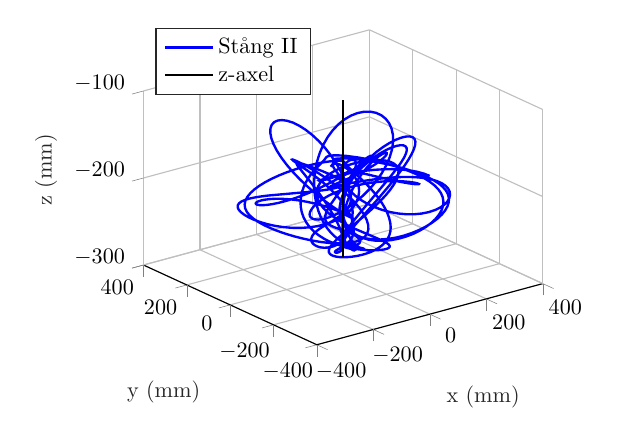
\begin{tikzpicture}[scale = 1.0, every node/.style={scale = 0.80}, domain = 0:2]

\begin{axis}[%
width=1.268\fheight,
height=\fheight,
at={(0\fheight,0\fheight)},
scale only axis,
xmin=-400,
xmax=400,
tick align=outside,
ymin=-400,
ymax=400,
zmin=-300,
zmax=-100,
view={-37.5}{30},
axis background/.style={fill=white},
axis x line*=bottom,
axis y line*=left,
axis z line*=left,
xmajorgrids,
ymajorgrids,
zmajorgrids,
legend style={at={(0.03,0.9)}, anchor=west, legend cell align=left, align=left, draw=white!15!black},
xlabel style={font=\color{white!15!black}},
xlabel={x (\text{mm})},
ylabel style={font=\color{white!15!black}},
ylabel={y (\text{mm})},
zlabel style={font=\color{white!15!black}},
zlabel={z (\text{mm})}
]
\addplot3 [color=blue, line width = 0.3mm]
 table[row sep=crcr] {%
306.442078083861	0	-213.809292879394\\
304.834152918501	25.6407131201611	-213.926168871957\\
300.034841087287	50.8337048254594	-214.268682406512\\
292.117571583297	75.1341279690336	-214.812733965986\\
281.206349710701	98.1034127531703	-215.519028875932\\
267.478224943102	119.313899323324	-216.334365748519\\
251.165416489434	138.354839892439	-217.193532793804\\
232.557499556417	154.840291302566	-218.022118974578\\
212.00314235969	168.419433215629	-218.739387748956\\
189.909260336279	178.788503570429	-219.263354337911\\
166.73800015467	185.704652532188	-219.515568478205\\
143.000378614293	189.001068875929	-219.425912555976\\
96.0464918001621	184.539065965547	-218.010028409112\\
53.593319357883	166.132206105253	-214.786474509195\\
19.8001774657893	136.336048649061	-209.866551824075\\
7.14993665520814	118.416733213679	-206.89127212324\\
-2.34463006200758	99.2886797821983	-203.66210348036\\
-11.6239395438735	59.9741859957706	-196.744434154324\\
-8.76612552912144	23.3405695144334	-189.721513440097\\
3.81793237739794	-6.55960584288516	-183.139260163799\\
12.7009655492652	-18.132781000372	-180.144957877856\\
22.6674232200143	-27.1898188942823	-177.410640671844\\
33.2189011079964	-33.6564883742071	-174.978072709658\\
43.8671790134601	-37.5547292520487	-172.885479986837\\
54.1509371429012	-38.9957551401706	-171.167839625154\\
63.6527820938977	-38.1720680617933	-169.856024757708\\
72.0149137298625	-35.346382400328	-168.975480442199\\
78.9030935141992	-30.8180982287557	-168.56417833244\\
84.0467256710986	-24.9383246793247	-168.658645708322\\
87.2538428916124	-18.0989828666451	-169.290421803944\\
88.4165118254007	-10.7161474798452	-170.485079038443\\
87.5132266651298	-3.2128578393187	-172.260985209928\\
84.6082154923208	3.99815262529603	-174.627834192687\\
79.8475896711236	10.5313216209294	-177.585010916759\\
73.4523040462457	16.0441646095382	-181.119898966059\\
65.7079828123355	20.2515939985396	-185.206282770048\\
56.9518103352996	22.9379651924443	-189.803035851877\\
47.5586738992301	23.9670589497152	-194.851662215574\\
37.9365771073478	23.2965271434481	-200.268136811679\\
28.49037893192	20.9755895073594	-205.952131180878\\
19.5935540444874	17.1346307726595	-211.793884437462\\
11.5725547359582	11.974462610426	-217.677878431215\\
4.69429585512626	5.75288156359613	-223.48735987289\\
-0.842770097227344	-1.23055481903134	-229.109461304314\\
-4.92070861734055	-8.66270549609635	-234.446595566953\\
-7.49997416988612	-16.2388774834531	-239.423163294755\\
-8.60772305987234	-23.6727183746765	-243.984789564203\\
-8.32851729546701	-30.7092826889759	-248.099509762141\\
-6.79203841310584	-37.131439719195	-251.756037674056\\
-4.16122213861252	-42.7634240828623	-254.961039859027\\
-0.621277903111093	-47.4721570598538	-257.73577361857\\
3.63033394270104	-51.1686926951957	-260.113289202967\\
8.39312879991428	-53.8045513460332	-262.133743682586\\
18.669458719829	-55.854277764114	-265.269810077073\\
28.733804406237	-53.8171671062189	-267.463814650897\\
37.3310628832884	-48.2754694481985	-268.98995215213\\
40.7619770788875	-44.4487506307113	-269.568737592318\\
43.4816450446086	-40.0807402599194	-270.050105864291\\
46.5054415974574	-30.2625626624341	-270.770053037901\\
46.0408821564341	-19.9592155820527	-271.208158555734\\
42.0543978333835	-10.3460282947586	-271.363051195677\\
30.1499896445072	0.317292922299998	-270.919800271802\\
13.1219386400784	3.52265739774526	-269.252011309833\\
0.564943826623448	0.259166237693478	-267.111046455084\\
-5.61820192151134	-3.17230979665931	-265.62815628456\\
-11.5067055798729	-7.8373482290628	-263.818076553698\\
-16.9205161211514	-13.7348846607381	-261.637911372872\\
-21.67859533403	-20.8437869879772	-259.041559456916\\
-25.5923693433403	-29.1141060491959	-255.985716378208\\
-28.4708494945691	-38.4640414707729	-252.432539023124\\
-30.3808980693628	-59.9033479821421	-243.72827210002\\
-21.2482600155088	-96.0953047269459	-226.650699165075\\
16.6535417394264	-140.416692341512	-198.414575501529\\
45.4859611514213	-154.749319716891	-183.969838375412\\
78.2533472767665	-160.472344149796	-170.847995675697\\
95.1351349946458	-159.565784318662	-165.129959962279\\
111.746939110752	-156.017600235121	-160.122470159231\\
127.610253267606	-149.835492019564	-155.914617812671\\
142.247640550185	-141.119776361219	-152.573779253391\\
155.201764414841	-130.063249789949	-150.144435373453\\
166.052387094926	-116.945650596663	-148.649243852614\\
174.432189315636	-102.125388637619	-148.090442448858\\
180.041272718248	-86.0288275836181	-148.451282029768\\
182.655642565046	-69.1355275715911	-149.699631173944\\
182.120780861231	-51.9599783398612	-151.800498025042\\
178.369520073079	-35.0453923477477	-154.7087591406\\
171.4329736041	-18.9495059107956	-158.366809977791\\
161.445905664045	-4.22647556996969	-162.704846241326\\
148.648995761912	8.59302109008303	-167.641078749751\\
133.387246783898	19.0229634516332	-173.082032179825\\
116.103844919418	26.6436293107961	-178.923104866375\\
97.328967636929	31.1225892698679	-185.049577790062\\
77.6490877102019	32.2277850365854	-191.344681572724\\
57.688043178563	29.8370634888155	-197.689080673924\\
38.10434172109	23.9553665999838	-203.954292552494\\
19.5476134524871	14.7113189502139	-210.014908333882\\
2.63388916157896	2.35271605510064	-215.75167748982\\
-12.0777117383573	-12.7632498905097	-221.05488238561\\
-24.1056768406004	-30.1845938485741	-225.827871362026\\
-33.0632534314231	-49.3834695744978	-229.990651163579\\
-38.6778542109166	-69.7908094878839	-233.488313577225\\
-40.7882883307606	-90.8129587303071	-236.289701407586\\
-39.34347525176	-111.852637648755	-238.38670089341\\
-34.3985545895768	-132.332929702417	-239.794213698012\\
-26.1044983708063	-151.714097717784	-240.547453834637\\
-14.6954702954547	-169.506964276508	-240.698565655281\\
-0.474886781814064	-185.282785577861	-240.312800084766\\
16.1990125030242	-198.680358549836	-239.464584875803\\
34.927027226267	-209.406523629949	-238.234100723804\\
55.280110190553	-217.232584206822	-236.702946369729\\
76.8105346854065	-221.999699482964	-234.950668921635\\
99.0624825623073	-223.617310455836	-233.052101344037\\
121.581205454778	-222.059872543041	-231.075078944934\\
143.920674184779	-217.362730774817	-229.078572731996\\
165.649759442718	-209.617586671475	-227.111258092604\\
186.358822575803	-198.96978998831	-225.210449761868\\
205.661449164705	-185.610798656108	-223.401380276826\\
223.187991000226	-169.76785351152	-221.697200041374\\
238.600020588819	-151.714633052091	-220.098484167789\\
251.595275514177	-131.767658366537	-218.593569668801\\
261.912101301525	-110.282258560118	-217.159747082174\\
269.334548554874	-87.648601491645	-215.765230929875\\
273.698396012277	-64.2872202121922	-214.371809816583\\
274.898126106451	-40.6433456450861	-212.938031569704\\
272.894582026473	-17.1793211736315	-211.422731907559\\
267.722221416579	5.63554255972684	-209.788727862637\\
259.492131537167	27.3375332424622	-208.008256238414\\
248.412674495456	47.4859992335368	-206.066538134679\\
234.776875010961	65.6834735587537	-203.962345524344\\
218.953553286522	81.5936683310491	-201.708316913465\\
201.378058088528	94.9592697196762	-199.330118042382\\
182.537737202675	105.618280490292	-196.864704346645\\
162.951625016349	113.516756257613	-194.357775918263\\
143.12840427821	118.701836267391	-191.857011900754\\
104.63362173217	121.588940819598	-187.053296559547\\
70.1726906528824	116.337467396031	-182.761469545704\\
41.6166491208542	105.749847293478	-179.182341494833\\
19.4809382578489	92.7205412973612	-176.408957840251\\
3.13244029697614	79.7473375524811	-174.465560344654\\
-8.8786207505679	68.6742359967151	-173.359525258259\\
-23.0113172528084	57.559200038403	-173.300338594201\\
-38.530284945287	52.6162084729248	-175.320549187764\\
-60.8193854690537	49.8882511654024	-179.729372803501\\
-70.1705307896327	48.3223647421044	-181.774210826659\\
-80.4280778244416	45.9589096854357	-184.113229391657\\
-91.4591451752081	42.5254325281046	-186.743069653805\\
-103.066047600936	37.7755870369272	-189.653781300312\\
-114.988454338375	31.5020844306202	-192.82672557544\\
-126.879840653209	23.5449446072308	-196.224927861503\\
-138.346693194255	13.8202709932418	-199.799782243832\\
-148.978572992002	2.33162921091633	-203.494654870528\\
-158.36733537748	-10.8280295060202	-207.246439297762\\
-166.127987843413	-25.4788099314354	-210.988515250387\\
-171.918036017388	-41.3610483280106	-214.654467109582\\
-175.457558305845	-58.1476918558029	-218.183023661148\\
-176.554729380524	-75.4656260500227	-221.525671235428\\
-175.101307150983	-92.9133142329148	-224.647896324264\\
-171.080170049677	-110.083098829576	-227.531469741946\\
-164.558167592652	-126.578966350205	-230.173776087603\\
-155.675476681478	-142.030235728678	-232.585804738191\\
-144.633985124894	-156.101628241114	-234.78928838171\\
-131.686136304302	-168.500749832364	-236.813464870041\\
-117.125466471502	-178.985259311412	-238.692017269883\\
-101.272613643692	-187.361219056568	-240.458221285653\\
-84.466271162116	-193.481998073266	-242.141838132253\\
-67.0570360151958	-197.248863264987	-243.767189141979\\
-49.4016507190453	-198.61137926627	-245.351668616285\\
-31.8573875611669	-197.567688781466	-246.904734110273\\
-14.7762770001468	-194.163778495422	-248.427520947352\\
1.50046354251856	-188.487118650167	-249.912480822092\\
16.6458766299988	-180.666554248316	-251.342821786008\\
30.3513871585131	-170.872302382215	-252.693531397081\\
42.3314304044834	-159.314585258577	-253.931741575171\\
52.328312596527	-146.241767205425	-255.017202065934\\
60.1172142749883	-131.937804518918	-255.902910930891\\
65.511200133863	-116.718902741214	-256.535903849666\\
68.3660696104584	-100.929310391423	-256.858204875758\\
66.1218202214691	-69.1237809257975	-256.320619427974\\
30.5485499506214	-15.5917283186716	-248.746799734871\\
16.0628409332274	-6.56537980067384	-245.193804643206\\
-0.087386675622156	0.0274243783688348	-240.91985182348\\
-17.5000556371335	3.91662449255585	-235.929156676631\\
-35.7154391435238	4.897001114484	-230.249760371705\\
-54.2260745219946	2.84110463538161	-223.935558122191\\
-72.489794671728	-2.28928376163503	-217.067276118452\\
-89.9576747462752	-10.4353213681514	-209.746020898604\\
-106.071766279944	-21.4358388037053	-202.099883071069\\
-120.291344930122	-35.0229225132976	-194.279636563393\\
-132.138032065227	-50.8315597514778	-186.442288842613\\
-141.213506103824	-68.4144505557308	-178.745766057893\\
-147.213288467961	-87.2597648085081	-171.344331115866\\
-149.936093514641	-106.810714692866	-164.384929563902\\
-149.28860336837	-126.485752100709	-158.004539079803\\
-145.285987069165	-145.698360218036	-152.3284054801\\
-138.061248076225	-163.890506898312	-147.455552738546\\
-127.841048824206	-180.538188874517	-143.471258708997\\
-114.934489161165	-195.161443587304	-140.45088999159\\
-99.7299142144877	-207.347122555252	-138.450398373776\\
-82.6795019728874	-216.759039326825	-137.506560876147\\
-64.2834941909748	-223.145565438137	-137.637156874553\\
-45.0742940167721	-226.345127224154	-138.84094035174\\
-25.6002849202633	-226.288789732623	-141.098083763913\\
-6.40952326325584	-222.987543288464	-144.379456054517\\
11.9611354887161	-216.545071772757	-148.637659903157\\
29.0024176914385	-207.159611525834	-153.803459768424\\
44.2498059750213	-195.118213899008	-159.78635899877\\
57.3002712453315	-180.7897914244	-166.474511096066\\
67.8282349055901	-164.614615444135	-173.735498400985\\
75.5996513679495	-147.089726762801	-181.418550076889\\
80.4748339109067	-128.737519782728	-189.36713744486\\
82.4169267140502	-110.09739067581	-197.415311570176\\
81.4876643632665	-91.6982254442573	-205.399583108865\\
77.8366611029251	-74.0349683269544	-213.168597278074\\
71.6915210129704	-57.5550220512131	-220.587008384677\\
53.1470229927696	-29.6322266558141	-233.930337886024\\
15.2633697685533	-4.0093443497401	-249.226335949586\\
-12.2056799555669	1.08970178877138	-256.121295685296\\
-25.5034536164246	0.130733489747456	-258.649013990311\\
-38.0786491495137	-3.00644253008255	-260.623847533739\\
-49.6494962726349	-8.15032858770695	-262.099151225555\\
-59.9678887535399	-15.096740149368	-263.130519721009\\
-68.8228714673294	-23.6149542430259	-263.773524371334\\
-76.0397963897185	-33.4527585710696	-264.081305631473\\
-81.4820495376648	-44.3416126908726	-264.103716593606\\
-85.0521569083082	-56.0018856957352	-263.88663290911\\
-86.6921680854208	-68.14803849216	-263.47137888832\\
-86.3833708189503	-80.4936429703873	-262.894259863922\\
-84.1459787650648	-92.7567777848018	-262.186312273283\\
-80.0387498427571	-104.666387392115	-261.373347708595\\
-74.1459988016504	-115.951216321846	-260.473327670913\\
-66.5879700790852	-126.353096524943	-259.498174230728\\
-57.5205365894324	-135.633930608915	-258.453669599526\\
-47.1319066831012	-143.579560855547	-257.339022608268\\
-35.6391640949648	-150.003105626574	-256.146669662513\\
-23.2847247240745	-154.747847638876	-254.862327603811\\
-10.3327542805477	-157.689775412305	-253.465314641562\\
2.93445387488549	-158.739884342929	-251.929153164331\\
16.2201882218141	-157.84633547863	-250.222464131316\\
29.2172088913652	-154.996546740199	-248.310156259\\
41.6119505517843	-150.219252310418	-246.154903852449\\
53.0896643244648	-143.587767056673	-243.719229212618\\
63.3521630834085	-135.247047329184	-240.975169124484\\
72.1294432861333	-125.400068693632	-237.906033653885\\
79.1884542429228	-114.297341197323	-234.507516466976\\
84.34719573927	-102.236378369526	-230.791251820664\\
87.4883333312023	-89.5543906845317	-226.7866144007\\
88.5723563754202	-76.6171328997292	-222.541360899047\\
87.6490104297073	-63.8035751990462	-218.12095773807\\
84.8566542450853	-51.4811037206067	-213.603616540943\\
80.4137686218597	-39.9815141713573	-209.073439914572\\
74.6140919623396	-29.5846062701745	-204.616667397614\\
60.3450098796965	-12.8402971046101	-196.234834865763\\
37.8573631732044	1.59449862838392	-185.866313176031\\
21.4257227555487	6.48346232525648	-178.80948106223\\
15.9527936609502	7.93708561853401	-175.94603776099\\
16.6194352083228	17.0211427141948	-174.098898664925\\
18.1141482359805	21.9681131815042	-174.346707089558\\
19.5955018451962	28.299735129726	-174.849693519392\\
20.7379669635836	36.0764692781385	-175.595325485701\\
21.2016811932737	45.2942881567062	-176.571981741246\\
18.7327988391403	67.6968372639933	-179.174786952056\\
15.157710805174	80.5312838368318	-180.779260370575\\
9.64455155774249	94.106770754849	-182.569506107442\\
1.96847376004405	108.071576426118	-184.527906647254\\
-8.02822171377125	122.012594753449	-186.631594188569\\
-20.4210849628692	135.466607941269	-188.851532845033\\
-35.1911140346285	147.938814497253	-191.152313071663\\
-52.2170061883057	158.924963455739	-193.492489396662\\
-71.2730397142477	167.935685183231	-195.825610093822\\
-92.0331419171864	174.52142439893	-198.102069090241\\
-114.081170932437	178.296161624004	-200.271826470672\\
-136.926823782473	178.958080624099	-202.287925493987\\
-160.029512076473	176.309457330213	-204.111185486731\\
-182.839978951196	170.281065846222	-205.71747968599\\
-204.806000916572	160.906523782669	-207.097285160332\\
-225.407538274628	148.330070383437	-208.2580055886\\
-244.176562396063	132.792282551449	-209.223103769825\\
-260.708422179236	114.611004693871	-210.02970350173\\
-274.667853980864	94.1625498955436	-210.725303318651\\
-285.790737163423	71.8645373292896	-211.363888719945\\
-293.887150609161	48.1618530983256	-212.001806076153\\
-298.833742432315	23.5123924720145	-212.693333167243\\
-300.567203437755	-1.62228589303464	-213.486039581376\\
-299.082007159515	-26.7833083418831	-214.417761925129\\
-294.427191688725	-51.5198818835419	-215.51432973772\\
-286.703938573171	-75.3938390131495	-216.787923375202\\
-276.064005489629	-97.9839556701727	-218.236110717531\\
-262.706537949593	-118.889572305772	-219.842163142986\\
-246.87197690755	-137.731763338147	-221.575526782472\\
-228.847298119454	-154.159165775345	-223.391339932413\\
-208.965444312006	-167.85382540223	-225.232378711474\\
-187.604242220925	-178.538256903776	-227.030560192734\\
-165.184106429917	-185.983586173796	-228.708983078651\\
-142.163998420697	-190.018486797724	-230.184505203863\\
-119.035219047128	-190.538479820077	-231.370812222943\\
-96.3126822445622	-187.514942864252	-232.181897643338\\
-74.521595210227	-180.998346728787	-232.53630629375\\
-54.1886743402191	-171.133487658833	-232.363598408946\\
-35.8239314865206	-158.163495885845	-231.607705175986\\
-19.9004075559812	-142.426814137415	-230.22995691395\\
-6.83500658485718	-124.353975699099	-228.211890321232\\
3.03094408799706	-104.459889200155	-225.557244738766\\
9.45025482356772	-83.3313084636956	-222.293018985004\\
12.2862720918309	-61.609491230361	-218.469534155176\\
11.52580067268	-39.9684348664719	-214.159535159192\\
7.28484469400109	-19.0829685224473	-209.453835224785\\
-0.204801172779469	0.425503793734492	-204.445417581579\\
-10.5927971313616	17.9756619563041	-199.239789460855\\
-23.4300993057632	33.0691541532819	-193.945614141359\\
-38.1917641034104	45.3119354718625	-188.670021489589\\
-54.3012574731615	54.4258443302368	-183.516015898532\\
-88.150703026021	62.7603066833253	-173.953625682409\\
-120.277763492239	58.2313162495496	-165.939891526209\\
-146.556180470063	42.6268232059843	-160.053897454583\\
-156.477236820011	31.5779999167078	-158.06929828223\\
-163.872130731038	18.9645331093332	-156.79315166828\\
-170.488876030161	-8.9789238194852	-156.52062076231\\
-160.105481892481	-50.2932881850216	-162.126829246344\\
-141.632230304102	-72.3363648150455	-169.837860208115\\
-129.869786612612	-80.7204333573131	-174.767839693516\\
-116.957087162465	-87.0851213619553	-180.31185939364\\
-103.322914166713	-91.3450764516615	-186.366162442482\\
-89.3939618947662	-93.5032597674141	-192.809135831836\\
-75.5706398770224	-93.6394427702006	-199.509466369375\\
-62.2207214156105	-91.910581866343	-206.323977516506\\
-49.6550329794669	-88.5248120622222	-213.114551631884\\
-38.1221980510864	-83.7260652664061	-219.753538056899\\
-27.8078012411696	-77.7808902061452	-226.127525939207\\
-18.8358898069558	-70.9665504231739	-232.140433130435\\
-11.272240304323	-63.5606195905954	-237.715722288217\\
-5.12751913965161	-55.8174408529582	-242.805313777024\\
-0.368766312435184	-47.958696184241	-247.389461104764\\
3.06911646198563	-40.1848286157607	-251.465090668853\\
5.27704742058921	-32.66989027764	-255.04437697612\\
6.36508940885801	-25.5602110786256	-258.151719180255\\
6.45616896858689	-18.9739847263524	-260.820641941628\\
4.17094375649492	-7.71152732319155	-265.004002224822\\
-0.51614091582087	0.660065818743078	-267.926401031817\\
-19.0193154149553	8.12341435531641	-271.920039609388\\
-23.9021885098765	5.74366903792225	-272.313955949076\\
-27.1344561102872	1.84786488344741	-272.424686823442\\
-28.3841151111646	-2.8432350687973	-272.28887830718\\
-27.522847406261	-7.54815067787263	-271.896191089868\\
-24.6375128161009	-11.4637466595877	-271.187064399444\\
-20.0424698949728	-13.8101013064922	-270.04849651015\\
-17.2663677127006	-14.1709025516653	-269.267148014553\\
-14.2823824458446	-13.8815175715553	-268.307893445278\\
-11.1922935810967	-12.8718971052199	-267.13808785066\\
-8.11328594693589	-11.0856537725968	-265.721824545205\\
-5.17599193984171	-8.48252066659575	-264.020476621599\\
-2.52227116132065	-5.04052923802698	-261.993499600969\\
-0.302769946693843	-0.757928000556092	-259.599504807616\\
1.3257194859558	4.34512360641207	-256.797601734369\\
2.20277595254584	10.2235024674933	-253.549707418529\\
2.16674981198088	16.7951786038448	-249.827733980966\\
1.06327021735171	23.9396490176333	-245.617030123274\\
-1.24581220221785	31.4986576562093	-240.918843400549\\
-4.87328162008879	39.2760439365921	-235.753386463868\\
-16.3463356219547	54.5229998119313	-224.209746936422\\
-33.352775546544	67.4689823049655	-211.592317597365\\
-54.8388964669986	75.6979359358646	-198.823910832081\\
-111.999647346726	64.7636381780745	-172.701134504699\\
-120.845332765309	56.9442144957014	-169.223411154577\\
-127.927477274211	47.633018385334	-166.447997655984\\
-132.944130032802	37.1548618000222	-164.387556355194\\
-135.655936369692	25.893532767006	-163.042077665985\\
-135.897905862074	14.2795868835119	-162.399793820115\\
-128.731173026038	-8.13897731704844	-163.127917918237\\
-100.282306052027	-32.6646109042177	-168.69117734079\\
-72.5342811279697	-38.0133619972038	-174.86451066467\\
-57.2545577624849	-36.4273218896985	-178.534935289504\\
-41.7309722088533	-31.7605225618447	-182.512230240851\\
-26.5331582625404	-23.9594131288935	-186.727429698992\\
-12.2471276835504	-13.0830073503772	-191.105876672962\\
0.547340211917515	0.693005186551432	-195.567727177271\\
11.3035795407971	17.0818098182764	-200.029895149568\\
19.5195305974136	35.6740786656748	-204.399076326361\\
24.7721768894848	55.9601185064532	-208.580281419946\\
26.7408378294853	77.3549379324393	-212.48213272252\\
25.2207163238033	99.2217131837187	-216.019864641406\\
20.1308955031653	120.897778270348	-219.118688182537\\
-0.456494908033562	161.058747934507	-223.771234866345\\
-98.1157804740756	218.291103588582	-225.880472468703\\
-121.863176472099	219.750820743869	-224.974722193578\\
-145.79548851754	217.633256467827	-223.796072373579\\
-169.406104855936	212.008585154927	-222.430878164601\\
-192.218524707764	203.018609921376	-220.964261557368\\
-213.79309497245	190.865985191867	-219.476209607603\\
-233.724818858752	175.799425653566	-218.039125370319\\
-251.650298811117	158.111801595384	-216.714346602436\\
-267.250580970386	138.133854230815	-215.549923338801\\
-280.251870455719	116.227727654406	-214.579180279839\\
-290.425827476424	92.7817464507411	-213.819855369541\\
-297.589958804727	68.2062667439678	-213.273805624131\\
-301.608523804684	42.9302799450158	-212.927270179819\\
-302.392622293646	17.3982384496356	-212.752307057959\\
-299.899647028653	-7.93246020640152	-212.707731562961\\
-294.143002492389	-32.5941529144217	-212.740134880913\\
-285.198354956024	-56.115096868489	-212.787383681704\\
-273.209111281194	-78.0280996304557	-212.782184827777\\
-258.391549499476	-97.8818727815468	-212.656260165571\\
-241.038551274735	-115.255391982843	-212.34489801696\\
-221.520699644107	-129.775165284176	-211.791586568059\\
-200.281626869501	-141.133566081072	-210.952398944241\\
-177.82514861423	-149.104397047053	-209.800897190398\\
-154.712595357528	-153.569203988726	-208.330744748143\\
-131.529197018936	-154.521884950966	-206.553831624365\\
-108.85982602927	-152.073838445592	-204.498520027722\\
-87.2643056528724	-146.454721222367	-202.207207224708\\
-67.2519091684501	-138.006972167267	-199.733406876912\\
-49.2559089412104	-127.171586395058	-197.138117798504\\
-33.605629878585	-114.445594300985	-194.480781350354\\
-20.5222487409822	-100.365804933582	-191.818001550607\\
-10.114978388389	-85.4841589448635	-189.202320690602\\
-2.38278515327136	-70.3405980674701	-186.680630068598\\
2.77731190680885	-55.4398535856591	-184.293582538508\\
5.5571268152114	-41.2318540686642	-182.075519638643\\
6.22069882636185	-28.0969636018917	-180.054812464832\\
5.08736106018995	-16.3416652569268	-178.255569481621\\
2.51631332872518	-6.19691817028541	-176.69963603091\\
-1.10790497402832	2.18303643953357	-175.408082618621\\
-5.38963164653148	8.72106659154434	-174.401751262631\\
-9.93579518860628	13.415620012862	-173.701546636753\\
-14.368793354887	16.3371262199733	-173.328575369864\\
-18.338330240216	17.6225781900728	-173.304125497616\\
-21.5325856403837	17.4689494718823	-173.649271605415\\
-23.6909639847115	16.1267781165449	-174.383182866495\\
-24.5882983541034	13.8749517746942	-175.531295284976\\
-24.061103269567	11.0300563986384	-177.116835568282\\
-18.4650897937611	4.95168585522958	-181.66101042814\\
0.160671317615311	-0.00164728074372533	-191.901899678822\\
8.26809257987111	0.610164732355827	-196.14532377493\\
16.8010662892892	2.66964755141385	-200.729055037151\\
25.386558551715	6.25278828447836	-205.585610694333\\
33.6256478157866	11.3455279854258	-210.62743570162\\
41.1331711656205	17.8449284031944	-215.757280966116\\
47.5676305473376	25.5706003704593	-220.876021707197\\
52.6452667797859	34.2782753484434	-225.886874785721\\
56.1500085783525	43.6752599835682	-230.699798261096\\
57.9396153820147	53.4369668143343	-235.235891556839\\
57.957254750699	63.233709543827	-239.436185646705\\
56.2243168580716	72.748464737325	-243.263576960391\\
52.8279200375051	81.6878765436238	-246.700435919645\\
41.6575554510059	96.8447384194073	-252.418776643705\\
7.89483075768823	111.705048906332	-259.987394636599\\
-1.4928978971559	111.755970182011	-261.288612531534\\
-10.7674209375921	110.342458018648	-262.424054436021\\
-19.6983145966502	107.52402674094	-263.421976418398\\
-28.0702734565939	103.390930100694	-264.305464133722\\
-35.6866373335257	98.0615413685342	-265.092185627288\\
-42.3707890690331	91.6755098678337	-265.793919073519\\
-47.9679330760964	84.3922566827877	-266.416398126239\\
-52.3468978118969	76.3888712592429	-266.959965371761\\
-55.4016226994586	67.857356806988	-267.419820043603\\
-57.0525529248149	59.0019125434987	-267.786211155347\\
-57.2478235014051	50.0360173056796	-268.044601744918\\
-55.9641811463663	41.179332442063	-268.175802475734\\
-53.2075965409591	32.6544539967832	-268.156075805007\\
-49.0135255963982	24.6835553300691	-267.957214701073\\
-43.4467863776086	17.4849713400391	-267.546602652114\\
-36.6072473076924	11.2716989883597	-266.888918827561\\
-28.6162329111685	6.24250166258759	-265.943132557913\\
-19.6164575929344	2.58185508954597	-264.662497393743\\
-9.78282692695655	0.459626537439078	-262.998351798043\\
0.678888718318888	0.0251083545069264	-260.901675318504\\
11.534423310326	1.40115608677093	-258.325019467952\\
22.5244071978976	4.67859079491097	-255.224772774853\\
33.3687401034557	9.9110154253118	-251.563690267378\\
43.7718870222045	17.1101829160327	-247.313587396418\\
53.4290304094181	26.2420429054949	-242.458069306768\\
62.033009392205	37.2235887738787	-236.995141628147\\
69.2819759589651	49.9206305839882	-230.939532337715\\
74.8824224932753	64.1421185799817	-224.329003895787\\
78.5420058705182	79.6198206860375	-217.242568886362\\
80.0086908017681	96.0242433723628	-209.783496685872\\
79.086462224815	112.974542903238	-202.074323808524\\
75.644963355339	130.047072684945	-194.253847561019\\
69.6282144354726	146.786084309079	-186.47326133438\\
61.0616983080703	162.716172395165	-178.891970812364\\
50.0579895152078	177.358101026539	-171.672041517649\\
36.8226939754895	190.264495322951	-164.959384664443\\
21.643121560499	201.017446687622	-158.892391899391\\
4.88464947211037	209.256987844218	-153.591181538615\\
-13.0218519508996	214.698747790276	-149.152591856218\\
-31.5960033762854	217.143149694484	-145.649769458079\\
-50.3246909169782	216.481414843042	-143.132620132265\\
-68.6791181575671	212.698678754453	-141.628773736243\\
-86.1324286108409	205.875980027801	-141.143319216283\\
-102.168579591325	196.171773754664	-141.673308291359\\
-116.295495925014	183.825775467888	-143.204677319578\\
-128.063119747292	169.163358096201	-145.70622359815\\
-137.079573313805	152.589247617901	-149.1298914237\\
-143.027142982426	134.578545780184	-153.410867272645\\
-145.677582796831	115.664663833039	-158.467617879732\\
-144.905954881954	96.4238404765269	-164.202065856552\\
-140.701657156088	77.4559677428078	-170.500335788515\\
-133.15308437544	59.352233497527	-177.246710400042\\
-122.464180631709	42.6863585381388	-184.312650538344\\
-108.956030394094	27.9925333674808	-191.557196287974\\
-93.0470930546527	15.7386304330635	-198.836332168185\\
-75.2391618851797	6.3080843063164	-206.006058691155\\
-56.0992277372252	-0.0152196140603564	-212.926143344824\\
-36.2381013168488	-3.0580200675671	-219.464388599125\\
-16.2778374775287	-2.76243211375373	-225.505156610741\\
21.5629096881303	7.52913464421044	-235.747079018438\\
53.1034964774969	29.2709205788854	-243.190804549275\\
65.4389245369845	43.5958514591246	-245.826310770125\\
75.0693455061829	59.6697794072219	-247.76171140527\\
81.7875984487835	77.0401243396641	-249.037408771035\\
85.4693547227131	95.2435651686216	-249.708511244324\\
86.0654518769003	113.81534427769	-249.83940470272\\
83.5976372147672	132.299806669424	-249.499383999815\\
78.1537579355288	150.260363403684	-248.75993242535\\
69.8816235074165	167.287758952543	-247.692161725474\\
58.9821537981803	183.006788887384	-246.364521241352\\
45.7021600385104	197.081504460607	-244.840829310446\\
30.3282689936333	209.227322321657	-243.178984250006\\
13.1752971885911	219.19679186026	-241.428576057967\\
-5.41650465974487	226.767439283499	-239.630346917697\\
-25.0813420608707	231.769404951321	-237.816506858894\\
-45.4355001453404	234.086305434611	-236.009510328657\\
-66.0842683160865	233.655006881416	-234.221381776315\\
-86.6281678390638	230.465030640144	-232.453625728553\\
-106.668683548892	224.557868076381	-230.697719775754\\
-125.813788226647	216.026377313486	-228.936172412769\\
-143.683600467206	205.014304457895	-227.144108810268\\
-159.916525280385	191.715824531746	-225.291325314582\\
-174.176183922838	176.37484475785	-223.344727598464\\
-186.159340897177	159.283670358208	-221.271038865377\\
-195.608145063761	140.782867914308	-219.041433604728\\
-202.333565478134	121.263211156738	-216.6373566059\\
-206.220510388653	101.147799242991	-214.05119784602\\
-207.234997675662	80.8773889254443	-211.28850653555\\
-205.432659074949	60.8952947655555	-208.368790069083\\
-200.964107225776	41.6289325873151	-205.325217046179\\
-194.075835735068	23.4687126102705	-202.203250593278\\
-185.091596333305	6.74495334012386	-199.055914175008\\
-174.38999491435	-8.28819941922541	-195.938110035391\\
-162.390212613956	-21.462922856057	-192.903701857775\\
-149.521855040202	-32.7025166125985	-190.001149179453\\
-122.82004205991	-49.5058469908414	-184.746428808516\\
-97.1458395542281	-59.6927285923301	-180.394195037287\\
-47.1257522498324	-68.8498345740409	-173.768310574338\\
-39.7172869160558	-69.9648440576444	-173.13844393528\\
-32.9261155618029	-71.3421731356657	-172.722966374462\\
-26.5697307330331	-73.1331018815349	-172.517215154875\\
-20.4420041173314	-75.4557022805138	-172.520074586116\\
-14.3150136213878	-78.3789749436315	-172.731821983305\\
-7.94896780047833	-81.9193115819395	-173.154152109816\\
6.45579718041688	-90.6445588504092	-174.643611371389\\
35.3591888365028	-105.690333502144	-178.556630443417\\
75.9411448774768	-117.288271761854	-184.554962150753\\
109.092574160023	-118.894833351512	-189.616248301313\\
145.030919606548	-112.683404313828	-195.281308388799\\
180.702840492656	-97.0128240119651	-201.201566554347\\
212.456184978657	-71.5558198301707	-206.969156777566\\
225.738861081994	-55.4702849037964	-209.682153319624\\
236.775920842136	-37.491397454479	-212.240501466266\\
245.268529297518	-17.9664081407627	-214.630711460881\\
250.996430095922	2.7095426624748	-216.853015240817\\
253.818736916295	24.1115238880458	-218.920104300551\\
253.671215972531	45.8006868107193	-220.854925090203\\
250.568205434617	67.3393112349662	-222.688444807509\\
244.595714438893	88.3042017614977	-224.45575396007\\
235.894413089059	108.293309889856	-226.190699416337\\
224.655712914122	126.931924794094	-227.923049188791\\
211.116255554716	143.877547962977	-229.676026961579\\
195.552955461679	158.824161978299	-231.464353157706\\
178.278435271125	171.506319466871	-233.292881912706\\
159.635266406267	181.701880632649	-235.156387158014\\
139.987376674725	189.229906664929	-237.038574962718\\
119.718729388944	193.954425899101	-238.912072584145\\
99.2302995689875	195.788383969076	-240.739526734499\\
78.9353963403033	194.696985471932	-242.474155641666\\
59.2540583956436	190.700929402235	-244.060641504066\\
40.6064210579191	183.879258926751	-245.436363359172\\
23.4050342184212	174.371513045632	-246.532964204087\\
8.04619746682948	162.378854933449	-247.278237547426\\
-5.09953216055158	148.163860204841	-247.598306920735\\
-15.6974176226714	132.048678145947	-247.420057428125\\
-23.4586735234449	114.41031107503	-246.67391717183\\
-28.1500214707435	95.6741921148194	-245.298844784434\\
-29.6068702270766	76.3176505507346	-243.24646146651\\
-27.7446150008401	56.8560868787608	-240.484019808168\\
-22.5682657137734	37.8293771618621	-236.997765883218\\
-14.1799579135391	19.7862745373258	-232.795750346992\\
-2.78352437555458	3.26652116536002	-227.909873134027\\
11.3145751233597	-11.218774115172	-222.397000940045\\
27.7087905555339	-23.2079174076318	-216.338930953172\\
45.9148265361424	-32.317785702732	-209.833933688075\\
65.364988107166	-38.2456467151507	-203.003249374543\\
85.4366876207288	-40.7956057394499	-195.982970739892\\
105.487408665925	-39.8944808762031	-188.913785323561\\
124.880172872289	-35.5923091671419	-181.936603150958\\
143.00772726998	-28.0573430657738	-175.188912266709\\
159.314165286719	-17.5661935599881	-168.801959768335\\
173.31301106109	-4.49009190665868	-162.898757677874\\
184.607856768041	10.7219634754605	-157.588763907628\\
192.903465582942	27.5642436166636	-152.965333367071\\
197.988279873444	45.4910993749995	-149.120095113684\\
199.758534893555	63.9359225273118	-146.129873662501\\
198.216451847495	82.3315879157823	-144.055688434024\\
193.464218328996	100.128938450421	-142.942514280181\\
185.695733318551	116.813150298908	-142.818950624294\\
175.18670367864	131.918049253915	-143.696696933266\\
162.28020943821	145.035635739927	-145.572591846603\\
147.369377928225	155.818805925132	-148.43399665772\\
130.89927267718	164.00039161812	-152.246308787394\\
113.350279417832	169.400037999234	-156.952860511943\\
95.2220170757528	171.929811348605	-162.474269226216\\
77.0163255566054	171.597304900089	-168.708228137014\\
59.2194361056965	168.505592200619	-175.530262386906\\
42.2831115917734	162.846641803952	-182.797693264847\\
26.6058653202905	154.879362722477	-190.361305531068\\
12.5253655592703	144.932525910353	-198.060172803234\\
0.305658562090457	133.37412445354	-205.73873892122\\
-9.8653837321105	120.594658174524	-213.252798551057\\
-17.8753736685354	106.993703502812	-220.473321857193\\
-23.6846871813929	92.9674625948393	-227.289717000496\\
-27.3219865970644	78.8974018681257	-233.612374899829\\
-28.8722280206604	65.1266031593969	-239.382184161762\\
-28.4639331018479	51.9539884417296	-244.56951594451\\
-26.2638783511006	39.6428457913937	-249.163975626424\\
-22.4680778868579	28.4158490600075	-253.172898157268\\
-17.2935516775134	18.4537754618964	-256.618275991597\\
-10.9704258726924	9.89548172280035	-259.533494715177\\
-3.73458416540257	2.83911083618278	-261.960056334023\\
4.17595008465975	-2.65370133091045	-263.943595406167\\
12.5261407584781	-6.55596917341694	-265.531514201104\\
21.0857969640327	-8.87177639160859	-266.770012011556\\
29.63214217868	-9.63419481580883	-267.702822861444\\
37.9533686025216	-8.90375364387643	-268.370686395986\\
45.8519112845458	-6.76643704349652	-268.810938033139\\
53.1473723072768	-3.3312696729015	-269.057205127152\\
59.6790412692639	1.27243962209872	-269.13919674039\\
65.3073257247474	6.898051032392	-269.082563809962\\
69.9101773796538	13.3835303412145	-268.907962894046\\
73.3870423761377	20.5529461075137	-268.631451803576\\
75.6626934939193	28.2192994125033	-268.264958925061\\
76.6882723784444	36.1875788854505	-267.816093016203\\
76.4419782380138	44.2578294145729	-267.287935119687\\
74.9294379975939	52.2281856937972	-266.678817558184\\
68.2655618147946	67.0698472924157	-265.185916826023\\
50.4836258329469	83.7468457017241	-261.999965303658\\
35.0862451071553	89.2268160948344	-258.921102083793\\
26.8985019160747	89.8969121946353	-256.984911139515\\
18.6920887833473	89.0860752839664	-254.731405084657\\
10.7181510929565	86.767820820637	-252.124561269085\\
3.23611260505311	82.9605567591126	-249.134956665724\\
-3.49467915513543	77.7315827504386	-245.743142632592\\
-9.22483449210154	71.2002138221139	-241.942951532833\\
-13.726415756482	63.539449365371	-237.744422103142\\
-16.8068004478648	54.9783848227464	-233.177760799856\\
-18.3283621296644	45.8094632774802	-228.299154484233\\
-18.220082252434	36.3618608864764	-223.182999948643\\
-13.2099729357736	18.0290191485126	-212.600202959798\\
10.8252218226991	-7.45037208124785	-192.846656710872\\
24.7555702644995	-11.5023421145165	-185.028779864746\\
30.9054580975971	-11.3179043122292	-181.815381480112\\
36.0666535884477	-9.87025416243046	-179.092147329612\\
39.9684223833916	-7.40567750992363	-176.861605292119\\
42.4022395904209	-4.22419284897705	-175.116045754959\\
43.227905777864	-0.664819489939475	-173.840532878445\\
42.3742242260804	2.9087974003221	-173.016148652154\\
39.8417117293807	6.12152956345307	-172.621274148227\\
35.7037297563057	8.60006016788122	-172.632473395486\\
30.1055201492857	9.98621617578374	-173.025167281328\\
23.2611623640701	9.95009358980207	-173.774105933764\\
15.4503367789497	8.20372374913666	-174.85297834755\\
6.99727283939131	4.50514395929883	-176.238881893443\\
-1.73370520021007	-1.33432352227288	-177.911551777305\\
-10.3317986748143	-9.43133500387211	-179.847831562867\\
-18.3533967329798	-19.8193711577341	-182.021345716911\\
-25.338520021377	-32.4403765602626	-184.402105091328\\
-30.8293623567794	-47.1397915795137	-186.956036007263\\
-34.3902743575711	-63.6656302407804	-189.644524861933\\
-35.6283123117645	-81.6721334742396	-192.424092739192\\
-34.2132743187151	-100.728314151397	-195.246331495323\\
-29.8955807215086	-120.329722297107	-198.05760875543\\
-22.5194381124363	-139.898681173822	-200.795293863954\\
-12.0430508141769	-158.817980099505	-203.393883813597\\
1.45269593597072	-176.471981009269	-205.791205505672\\
17.7679366512493	-192.273889493658	-207.93155181851\\
36.5936300596642	-205.690803832783	-209.769101373468\\
57.52656010009	-216.265124048283	-211.271363090573\\
80.0891613247358	-223.633635864012	-212.422578441054\\
103.75835225141	-227.552323891801	-213.228507784244\\
127.985772243317	-227.88268459552	-213.715093688448\\
152.223089938512	-224.596767327381	-213.925688867379\\
175.942102695532	-217.767662990732	-213.917442359242\\
198.649213425635	-207.555219081554	-213.756876045356\\
219.89523453506	-194.191138296988	-213.515170214199\\
239.281270784212	-177.964798065051	-213.263493750608\\
256.461761871788	-159.210697392761	-213.068709633821\\
271.140654940945	-138.295247904703	-212.990013399028\\
283.07221214558	-115.610749756328	-213.075303417465\\
292.061047536411	-91.569878182755	-213.358933564264\\
297.961539214896	-66.6008198358495	-213.860234954176\\
300.677790092152	-41.1433100323241	-214.582633468985\\
300.164393883708	-15.6450665385898	-215.513368905767\\
296.427759718554	9.44191902211765	-216.623932692444\\
289.522067929538	33.6649099156519	-217.872193507104\\
279.554000892115	56.5734733986673	-219.201826167306\\
266.689641884204	77.7253970742624	-220.544628734323\\
251.157256641443	96.6947369597463	-221.823333009308\\
233.249680067287	113.081843531619	-222.954729842655\\
213.325174838466	126.525397214906	-223.853399453627\\
169.173623097474	143.412327098595	-224.625300547513\\
100.079088945775	141.413850079066	-222.271741426396\\
41.356002684039	108.510524981955	-215.20008280845\\
26.5415412438098	92.2269941044188	-211.918604161911\\
14.7512770076861	74.1800910721038	-208.284275530491\\
1.00595591454737	35.3309855875939	-200.286945369517\\
4.58522411288453	-20.1930099667844	-187.780950375018\\
20.1868083698707	-48.9543321885575	-180.048251115638\\
30.703177364413	-59.6974976172284	-176.568685148441\\
42.3619469001454	-67.7265351696871	-173.424830328139\\
54.6387267112744	-72.9483720435012	-170.671067337155\\
67.0141304859673	-75.3699392663737	-168.357777118262\\
78.9910308283235	-75.0921489575905	-166.53138840144\\
90.1098113145103	-72.3013061360977	-165.234320194417\\
99.9614195693451	-67.2585207711991	-164.504765503391\\
108.198194469358	-60.2876417827082	-164.376246249944\\
114.541733312777	-51.7617547743653	-164.877178725182\\
118.776505453477	-42.085032624027	-166.036422031791\\
120.769329864597	-31.6883671700514	-167.874477817045\\
120.47859138519	-21.0143915288783	-170.398803660896\\
117.954329181517	-10.4985014276618	-173.601991195948\\
113.334614648627	-0.550217386500151	-177.459979675207\\
106.838159830614	8.46441268136118	-181.930526016794\\
98.7532458590563	16.2385836211249	-186.95220070256\\
89.4221256232587	22.5375572468546	-192.444749573766\\
79.218341763449	27.2059404458901	-198.311870814619\\
68.5456473153865	30.1779994743391	-204.434100370959\\
57.7941145559382	31.4712313063282	-210.685848336133\\
47.3199825597414	31.1758560442468	-216.942304539273\\
37.4343079134215	29.4432531317417	-223.083766966902\\
28.3948609190589	26.4732591958065	-228.99995489945\\
20.401252215172	22.5012105871237	-234.59395131289\\
13.5928962824684	17.7853794802834	-239.785513834861\\
8.03652965258846	12.5752251862546	-244.524566814367\\
3.73802613550725	7.09770863385813	-248.78989088801\\
0.663829132078092	1.56649714565395	-252.576059690188\\
-1.25547740142258	-3.82810872687043	-255.893645959164\\
-2.11739539905153	-8.92275346394445	-258.766066376383\\
-2.04008599098455	-13.5832426540273	-261.226280871499\\
-1.15533298204656	-17.7053361632872	-263.313510273884\\
2.47797380112229	-24.0501690831881	-266.536299214682\\
7.65988623179567	-27.6230779036138	-268.755791706634\\
13.3178453438828	-28.4114668341794	-270.24371374151\\
18.4990496303519	-26.6852952868445	-271.210336851461\\
22.4171018652407	-22.934036332257	-271.800717556354\\
24.4709777824939	-17.8033476438363	-272.097114444552\\
24.2703037542431	-12.058920066312	-272.128669210429\\
19.4424042198016	-4.13146926104724	-271.622367725302\\
5.46231798789842	0.693477847204974	-269.407342343493\\
-3.66583592494783	-1.11037424931715	-267.254110512146\\
-8.42420663879454	-3.34550204116982	-265.81186259651\\
-13.155459862342	-6.54976511036824	-264.074537979306\\
-17.7276661280122	-10.7682403239409	-261.999408302588\\
-21.9930385384931	-16.0279654984517	-259.544008566893\\
-25.7908175368526	-22.3341292427686	-256.668034699087\\
-28.9507725770334	-29.6666375305446	-253.335609990835\\
-31.2972806312386	-37.9770740172876	-249.517844527543\\
-32.8489938073736	-57.1811205501542	-240.362107118231\\
-29.1248840485877	-78.9035585193382	-229.213168182754\\
-19.0660132652987	-101.447069682704	-216.415775857914\\
8.68786032640304	-131.493229226984	-195.839312764707\\
48.9698048344707	-148.905712179334	-176.746502224534\\
78.9985586773859	-149.705639374818	-166.578745474196\\
93.735567338259	-146.410739977931	-162.560598921271\\
107.676804607784	-140.650349276756	-159.336006725399\\
120.365812675366	-132.538463916235	-156.939852348156\\
131.369403011112	-122.279365241047	-155.386511370539\\
140.295823485496	-110.162343127218	-154.670720327808\\
146.801183396002	-96.5458723594875	-154.776204906988\\
150.597486794998	-81.8475732524161	-155.679835890409\\
151.47047178898	-66.5394711284954	-157.347371225402\\
149.290793117894	-51.1351094289495	-159.73424432127\\
144.023376796061	-36.1743749323255	-162.786198806201\\
135.734513840445	-22.2061879854022	-166.439739656233\\
124.596067580227	-9.76927143622999	-170.622480499532\\
110.886105260411	0.628582423758985	-175.253494611877\\
94.9746356026624	8.53111573538467	-180.248052538786\\
77.3095261609905	13.5495037425449	-185.519341096164\\
58.4292158304557	15.3819382260113	-190.968518466813\\
38.9339285555662	13.8307924876167	-196.490950654421\\
19.4644630752878	8.81513381113859	-201.977811390228\\
0.677974058673897	0.378488131448933	-207.318220796196\\
-16.7782938898275	-11.3090365660224	-212.402067766072\\
-32.2949780681108	-25.9557194972225	-217.123996359279\\
-45.3345835614503	-43.1672317497813	-221.391240370924\\
-55.4386183913255	-62.4533977774196	-225.121956353845\\
-62.2548090047305	-83.2577720456869	-228.254077937399\\
-65.5474515667922	-104.984521432264	-230.748212334662\\
-65.1985408292088	-127.022380798551	-232.588026326131\\
-61.2039118297791	-148.766935875032	-233.779680541435\\
-53.6652212805324	-169.640273253881	-234.350322304624\\
-42.778799582125	-189.107517712914	-234.345756635019\\
-28.8234479026864	-206.697993395667	-233.829473599629\\
-12.1418520273068	-222.00415194953	-232.877242572886\\
6.87321503858567	-234.685522163813	-231.570936435434\\
27.7921034728876	-244.475321509929	-229.995124239268\\
50.1616442344924	-251.180162395224	-228.233387495088\\
73.516907920677	-254.677690954158	-226.36502251806\\
97.3911523356932	-254.91279008886	-224.462231349487\\
121.325772867986	-251.896784842689	-222.587565215276\\
144.873821495143	-245.694152155356	-220.792316998925\\
167.596559110531	-236.409162157876	-219.116517835258\\
189.074807221723	-224.200962759152	-217.586808308244\\
208.913705152336	-209.279443987213	-216.215511956311\\
226.746570629694	-191.90127248259	-215.000512801129\\
242.238705237347	-172.366718550692	-213.925895815652\\
255.091698118525	-151.017041878924	-212.963321195523\\
265.04866878544	-128.232000275368	-212.074080883168\\
271.900712529378	-104.426880527737	-211.211758728209\\
275.494576389915	-80.0483409220287	-210.325383294326\\
275.73480201047	-55.5670089693919	-209.36387816366\\
272.60509642935	-31.4729960043431	-208.281064785875\\
266.181940988709	-8.26166060606243	-207.039052030717\\
256.629565965114	13.5854047293314	-205.611811504124\\
244.203444441075	33.6181306715459	-203.987229298457\\
229.249526475667	51.4381481559976	-202.168172297518\\
212.198101846537	66.7201873872962	-200.172511348059\\
193.551570747667	79.2331045060874	-198.032144758543\\
173.865772553883	88.8586055971801	-195.791148153559\\
153.693625245427	95.5859309232529	-193.497330990004\\
113.957335322939	100.801782537071	-188.934592683674\\
77.9943395540524	96.696310273155	-184.683376858411\\
48.2592347454686	86.0911203192441	-180.997921510977\\
25.7701389315391	72.143104539187	-178.034196030361\\
17.1924992922491	64.8458192826353	-176.850191726911\\
10.228991587147	57.7692164400598	-175.875597355445\\
0.336217071081592	45.324890786253	-174.586678702969\\
-5.88332194987964	36.3606331262872	-174.237352018399\\
-10.7301744985982	31.5067943656893	-174.915570241868\\
-16.5062203045389	30.4980581607851	-176.738367100758\\
-20.3808932154055	31.1082055551098	-178.118649538469\\
};
 \addlegendentry{Stång \rom{2}}

\addplot3 [color=black, line width = 0.3mm]
 table[row sep=crcr] {%
0	0	-280\\
0	0	-100\\
};
 \addlegendentry{z-axel}

\addplot3 [color=black, line width = 0.3mm]
 table[row sep=crcr] {%
0	0	-280\\
0	0	-100\\
};
\end{axis}
\end{tikzpicture}%
 %   \caption{Simulerad position för stång \rom{2}s ändpunkt under 10 s med samma initialvillkor som i mätning fyra. Notera att systemet uppvisar kaotiskt beteende under hela simuleringen, även om den är längre än vad som kunde uppmätas experimentellt.}
%    \label{fig:3dfig}
%\end{wrapfigure}

%
\markright{Eric Lindgren, Simon Pettersson Fors, Grupp 47, Uppgift 2}

%\noindent Som har nämnts ovan observeras en skillnad  är de tidsintervall där kaotiskt beteende kan observeras i de uppmätta fallen begränsade.

%Som har nämnts ovan observeras att de tidsintervall inom vilka tydligt kaotiskt beteende kan identifieras är relativt korta även om de blir längre för högt $\omega$. Detta kan orsakas av interna dämpningar inom systemet, exempelvis i kardanknuten mellan stång \rom{1} och \rom{2}. Detta förslag styrks av att simuleringarna, vilka skildrar systemet i det ideala fallet utan sådana dämpningar, ej visar på att det kaotiska beteendet dämpas ut över tid. Se figur \ref{fig:3dfig} för ett exempel på en simulering under 10 s med samma initialvillkor som i mätning fyra.



 %Utifrån uppmätt samt simulerad data kan alltså slutsatsen att en dubbel konisk pendel kan uppvisa kaotiskt beteende dras.

%% tidsperioder där kaotimeskt beteende kan identifieras är dock inte särskilt långa, även om detta varierar från mätning till mätning vilket syns ovan. I vissa fall finner systemet ett nytt jämviktsläge när spoltråden lossas, medan det i andra tar betydligt längre tid (jämför ex. de två mätningarna ovan). Att det kaotiska beteendet upphör kan bero på interna dämpningar inom systemet, exempelvis i polhemsknuten mellan de två stängerna. Detta syns extra tydligt vid jämförelse med systemets simulerade beteende. Det simuelerade systemet uppvisar ett kaosartat beteende över längre tid vilket liknar det som det verkliga systemet uppvisar under kortare övergångsperioder. 

\vspace{-2px}
\section{Slutsatser}
Höghastighetskamerorna är ett alternativ till att använda en laserpekare för att uppmäta $g$ med en enkel konisk pendel. Dessa medför fördelarna att motorvinkeln experimentellt kan uppmätas och ett stort antal mätningar av $g$ kan åstadkommas under kort tid. Tyngdaccelerationskonstanten $g$ uppmättes till $9.83 \pm 0.06$ m/s$^2$ vilket avviker i medelvärde med $0.1\%$ ifrån det teoretiska värdet $9.8170$ m/s$^2$. Precision och systematiska fel föreslås kunna minimeras med en stabilare DC-motor och att ersätta kardanknuten med ett kullager.

Simuleringar och mätningar av en dubbel konisk pendel visar att ett sådant system kan uppvisa periodisk och kaotisk rörelse beroende på initialvillkor. Det är möjligt att vinkelhastigheten $\omega$ både kan stabilisera och destabilisera systemet och ett eventuellt samband för detta observeras vara icke-linjärt. Slutligen föreslås att längden för det tidsintervall där eventuellt kaotiskt beteende kan observeras möjligtvis kan förlängas genom att minimiera dämpningar i kardanknutarna.

\vspace{-2px}
\printbibliography

\appendix

\section{Tröghetsmatriser för de två stängerna och för kardanknut}

\markright{Appendix}

Med koordinatsystem ansatta utmed symmetrixlarna för respektive stång enligt geometrin i figur 1 och med användande av Steiners teorem fås tröghetsmomentmatriserna

%Kanske lägga dessa i appendix? :P
\begin{align}
\centering
                    I_{x\rom{1}} & = m_1 \left(\frac{L^2_1}{12} + \frac{r^2_1}{4}\right) + m_1\left(\frac{L_1}{2} +d \right)^2\notag \\ 
    \textbf{I}_{{\rom{1}}}:  I_{y\rom{1}} & = m_1 \left(\frac{L^2_1}{12}                 + \frac{r^2_1}{4}\right) + m_1\left(\frac{L_1}{2} +d \right)^2\\
                    I_{z\rom{1}} & = m_1 \frac{r_1^2}{2} \notag \\
                    \notag\\
                    I_{x\rom{2}} & = m_2 \left(\frac{L^2_2}{12} + m_2\frac{r^2_2}{4}\right) + m_2\left(L_1+d\right)^2 + 2m_2\left(L_1+d\right)\left(\frac{L_2}{2}+d\right)\cos{\left(\theta_2-\theta_1\right)}\notag\\
                    & + m_2\left(\frac{L_2}{2} +d\right)^2 \notag \\
    \textbf{I}_{{\rom{2}}}:  I_{y\rom{2}} & = m_2 \left(\frac{L^2_2}{12} + \frac{r^2_2}{4}\right) + m_2\left(L_1+d\right)^2 + 2m_2\left(L_1+d\right)\left(\frac{L_2}{2}                                  +d\right)\cos{\left(\theta_2-\theta_1\right)} + \notag\\
                    & + m_2\left(\frac{L_2}{2}+d\right)^2\cos{\left(\theta_2-\theta_1\right)}^2 \\
                    I_{z\rom{2}} & = \frac{r_2^2}{2} m_2 +m_2\sin\left(\theta_2 - \theta_1\right) \left(\frac{L_2}{2} +d\right)^2 \notag\\ \notag
\end{align}
$m_1$, $r_1$ och $m_2$, $r_2$ är stängernas massa respektive deras tjocklek. $d$ är längden på polhemsknuten mellan stängerna. Notera att tröghetsmomentet för den undre stången har ett implicit tidsberoende genom $\theta_1$ och $\theta_2$.

Analogt ges för kardanknuten om den moduleras som en ihålig cylinder
\begin{align}
\centering
                    I_{xk} & = m_k\left(\frac{L_k^2}{12} + \frac{r_1^2 + r_y^2}{4}\right) + m_k\left(\frac{L_k}{2} + d_k \right)^2\notag \\
                   \textbf{I}_\textbf{k}: I_{yk} & = m_k\left(\frac{L_k^2}{12} + \frac{r_1^2 + r_y^2}{4}\right) + m_k\left(\frac{L_k}{2} + d_k \right)^2 \\
                    I_{zk} & = \frac{1}{2}m_k\left(r_1^2 + r_y^2\right) \notag,
\end{align}
där $m_k$ är kardanknutens massa, $L_k$ dess längd, $r_1$ och $r_y$ är innerradie respektive ytterradie och $d_k$ är avståndet till vridpunkten.

\section{Förtydligade teoretiska härledningar}
Studera en enkel konisk pendel med stång med längd $L_1$, radie $r_1$ och massa $m_1$ samt kardanknut som modelleras till en ihålig cylinder med massa $m_k$, längd $L_k$, innerradie $r_i = r_1$ och ytterradie $r_y$, se figur 1 (a). Låt även stångens och modellen av kardanknutens översta punkter befinna sig $d$ respektive $d_k$ ifrån kardanknutens vridpunkt. Antag att motoraxeln är parallell med vertikalen samt att vinkelhastighet $\omega$ är konstant för jämnviktsläget och fixera ett roterande koordinatsystem med z-axel längs den cylindriska stångens symmetriaxel. Med tröghetsmomentsmatrisen $I$ för den enkla koniska pendeln uttryckt i det roterande systemet, se Appendix del A,  kan systemets rörelseenergi $T$, potentiella energi $V$ och Lagrangian $L = T - V$ tecknas
\begin{align}
    T & = \frac{1}{2}\left[I_{x\rom{1}}\dot{\theta}^2 + \omega^2\left(\sin^2\theta I_{y\rom{1}} + \cos^2\theta I_{z\rom{1}}\right)\right] \\
    V & = -m_1 g\left(\frac{L_1}{2} + d\right)\cos\theta - m_k g\left(\frac{L_k}{2} + d_k\right)\cos\theta.
    \label{eq: Lagrange_enkel}
\end{align}
Tillhörande Lagrangeekvation med avseende på $\theta$ är därför
\begin{equation}
    I_{x}\ddot{\theta} + m_1g\left(\frac{L_1}{2} + d\right)\sin\theta + m_kg\left(\frac{L_k}{2} + d_k\right)\sin\theta - \omega^2\sin\theta\cos\theta\left(I_{y} - I_{z}\right) = 0.
\end{equation}
För jämviktsläge gäller $\ddot{\theta} = 0$ varav $g$ erhålls som
\begin{equation}
    g = \frac{\omega^2\left(I_{y} - I_{z}\right)\cos\theta}{m_1\left(\frac{L_1}{2} + d\right) + m_k\left(\frac{L_k}{2} + d_k\right)}.
    \label{eq: g}
\end{equation}

Likt den teoretiska beskrivningen definierar vi en dubbel konisk pendel som en enkel konisk pendel med ytterligare en stel stång fäst i änden av den första. Den nedre stången är fäst vid den övre med en kardanknut av samma typ som fäster motorn till den övre stången sådan att den nedre stången kan rotera i samma plan som den övre, se figur 1 (b). Enligt samma metodik som för den enkla koniska pendeln kan Lagrangianen för den dubbla koniska pendeln tecknas som 

\begin{align}
    L & = T-V \\
    T & = \frac{1}{2}[\dot{\theta_1}^2\left(I_{x\rom{1}} + I_{x\rom{2}}\right) + \dot{\theta_2}^2 I_{x\rom{2}} + \dot{\theta_1}\dot{\theta_2}I_{x\rom{2}} + \\ 
    & + \omega^2\left(I_{y\rom{1}}\sin^2\theta_1\ + I_{z\rom{1}}\cos\theta_1^2 + \tag*{} I_{y\rom{2}}\sin^2\theta_2 + I_{z\rom{2}}\cos^2\theta_2 \right)] \\
    -V & = m_1 g \left(\frac{L_1}{2} +d\right)\cos{\theta_1} + m_2g[\left(L_1+d\right)\cos\theta_1 + \\
    & + \left(\frac{L_2}{2}+d\right)\cos\theta_2 ] \tag*{}
\end{align}
där $I_{\rom{1}}$ och $I_{\rom{2}}$ är den undre respektive den övre stångens tröghetsmatriser runt deras symmetriaxlar. Dessa matriser fås enligt Steiners teorem, se Appendix del A och uppmärksamma att $I_{\rom{2}}$ är tidsberoende. Under antagandet att den undre stången är mycket kortare än den övre (exempelvis en tiondel så lång) så betyder det att produkten $m_2 (\frac{L_2}{2} + d)$ är liten relativt $L_1$, varpå Lagranges ekvationer för $\theta_1$ och $\theta_2$ kan approximeras till 

\begin{align}
\frac{\partial}{\partial t}\frac{\partial L}{\partial \dot{\theta_1}} - \frac{\partial \tag*{} L}{\partial \theta_1} = 0 : \hspace{20px} & \ddot{\theta_1}\left(I_{x \rom{1}} + I_{x \rom{2}} \right) + \ddot{\theta_2}I_{x \rom{2}} - \\ 
& - \omega^2 \sin{\theta_1}\cos{\theta_1} \left(I_{y \rom{1}} - I_{z \rom{1}}\right) + \\ \tag*{}
& + g \sin{\theta_1} \left(m_1 \left(\frac{L_1}{2} +d\right) + m_2\left(L_1 + d \right)\right) = 0 \\ \tag*{}
\frac{\partial}{\partial t}\frac{\partial L}{\partial \dot{\theta_2}} - \frac{\partial L}{\partial \theta_2} = 0 : \hspace{20px} & \ddot{\theta_1}I_{x \rom{2}} + \ddot{\theta_2}I_{x \rom{2}} - \\
& - \omega^2 \sin{\theta_2}\cos{\theta_2}\left(I_{y \rom{2}} - I_{z \rom{2}}\right) \\
& + g \sin{\theta_2} m_2\left(\frac{L_2}{2} + d\right) = 0. \tag*{}
\end{align}

Tröghetsmomenten för stång två, $I_{x \rom{2}}, I_{y \rom{2}}$ och  $I_{z \rom{2}}$ approximeras även dem. Utöver detta har det även antagits att motorns rotationshastighet $\omega$ är konstant.  Dessa ekvationer kan lösas numeriskt med hjälp av Matlab för olika initialvillkor, se Appendix del B. 

\section{Matlabkod för analys av den enkla koniska pendeln samt för att beräkna g}

I följande avsnitt presenteras den matlabkod som har använts vid analys av den enkla koniska pendeln samt för att beräkna g.

%\subsection{Program för att beräkna $g$}

Nedan följande program läser in tabb-separerade filer från kamerorna och beräknar ett värde på $g$ för varje period. Först identifieras längden på varje period med hjälp av ett annat program som implementerar funktionen \textit{findpeaks} varpå rotationshastigheten $\omega$ under perioden kan beräknas. Därefter minsta-kvadratanpassas datan under perioden först mot ett plan i tre dimensioner och därefter mot en ellips i samma plan, varur pendelns vinkel $\theta$ mot vertikalen kan bestämmas. Efter detta används ekvation \ref{eq: g} för att beräkna $g$ för perioden, varefter processen upprepas för varje period. Sist sparas alla beräknade värden på $g$ till en ny tabb-separerad fil för senare felanalys av datan. 

\begin{lstlisting}[style=Matlab-editor]

clear all clc; clf; close all;

fileName = 'matning3_grunduppgiftV2_truncated.txt'; %File to save the edited data to

%Edit tsv-file to remove column headers etc
fid = fopen('matning3_grunduppgiftV2.tsv', 'r') ;              % Open source file.
61
%Skip the first 1 lines%%%%%%%%%%%%%%%%%%%%%%%%%%%%%%%%%%%%%%%%%%%% 
fgetl(fid) ;                                  % Read/discard line.
fgetl(fid) ;                                  % Read/discard line.
fgetl(fid) ;                                  % Read/discard line.
fgetl(fid) ;                                  % Read/discard line.
fgetl(fid) ;                                  % Read/discard line.
fgetl(fid) ;                                  % Read/discard line.
fgetl(fid) ;                                  % Read/discard line.
fgetl(fid) ;                                  % Read/discard line.
fgetl(fid) ;                                  % Read/discard line.
fgetl(fid) ;                                  % Read/discard line.
%%%%%%%%%%%%%%%%%%%%%%%%%%%%%%%%%%%%%%%%%%%%%%%%%%%%%%%%%%%%%%%%%%% 
buffer = fread(fid, Inf) ;                    % Read rest of the file.
fclose(fid);
fid = fopen(fileName, 'w')  ;   % Open destination file.
fwrite(fid, buffer) ;                         % Save to file.
fclose(fid) ;


data = tdfread (fileName, '\t') %Read truncated tsv-file.

xArray = data.New_0000_X;        %Extract x,y,z,t data
yArray = data.New_0000_Y;
zArray = data.New_0000_Z;
tArray = data.Time;



%Find max and min for x, y, 
figure(1000)
[max, locmax, min, locmin] = findPeaksOG(xArray, tArray, true, 'hej', 'hej'); %Only x-data so far
%Use the average of locmin and locmax as vector of locations
%loc = round((locmin + locmax)./2);
%plot(loc, xArray(loc), '*') %Position in which to plot diameter, omega
hold off

%Calculate diameter and halftime - dependant on x
fulltimeArray = calculateFulltime(tArray, locmax);
%Remove zeros - if uneven number of periods
fulltimeArray = fulltimeArray(fulltimeArray~=0);
figure(4000)

%Now loop through all periods (that is all locmax(i) -> locmax(i+1)
g = zeros(length(fulltimeArray),1);
thetaArray = zeros(length(fulltimeArray),1);
omegaArray = zeros(length(fulltimeArray),1);

%Parameters of pendulum
L1 = 205/1000;
m1 = 128/1000; 
r1 = 5/1000;
ry = 11/1000;
%Parameters for polhemsknut
Lk = 18/1000; %Avarage length of polhemsknut
d = 12/1000; %displacement down to turning point of rod
dk = 6/1000; 
mk = 35/1000; %hette m1 tidigare

%for calculating theta - with ball
L = 0.221; % pm 0.022

for i = 1:1:length(fulltimeArray) %
    if i+1 > length(locmax) %To avoid stepping out of bounds
        break
    end
    
    %Subarrays are calculated from max & min in x!
    subxArray = xArray(locmax(i):locmax(i+1)); %Extract the current sub array %x
    subyArray = yArray(locmax(i):locmax(i+1));                                %y
    subzArray = zArray(locmax(i):locmax(i+1));                                %z
    %Calculate mean square ellipse
    ellipse = calculateEllipse(subxArray, subyArray, subzArray);
   
    diameter = (ellipse.long_axis+ellipse.short_axis)/2/1000; %take mean diameter, convert to meters
    sintheta = diameter/(2*L);
    
    %Calculate the rotational speed for this period
    currentOmega = 2*pi./fulltimeArray(i); %2pi since whole period
    
    %g(i) = calculateG2(L1, r1, d, dk, m1, m2, currentOmega, sintheta);
    g(i) = calculateG3(L1, Lk, r1, ry, d, dk, m1, mk, currentOmega, sintheta);
    
    %Export data to plot
    omegaArray(i) = currentOmega;
    theta = asin(sintheta);
    thetaArray(i) = theta;
end

%Save last plot as a tikzpicture
figure(4000)
%cleanfigure('TargetResolution', 0.1);
%cleanfigure('minimumpointDistance', 10)
%matlab2tikz('ellips.tex', 'height', '\fheight');



%Now plot omega and theta and let the user choose the area in which to take
%mean of g


figure(2000)
yyaxis left
plot(omegaArray, 'r')
hold on
yyaxis right
plot(thetaArray, 'g') %Norm the plots towards mean 
hold off
%title('omega and theta for each period')
%xlabel('Period')
%ylabel('Normed value')
legend('Omega','theta')
%cleanfigure('TargetResolution', 5);
%cleanfigure('minimumpointDistance', 0.1)
%matlab2tikz('omegatheta.tex', 'height', '\fheight');
%cleanfigure
%matlab2tikz('omegatheta2.tex', 'height', '\fheight')

%pause
%[xFrames, yFrames] = ginput(2);
%firstFrame = xFrames(1);
%lastFrame = xFrames(2);
%round to nearest deci
%firstFrame = round(firstFrame);
%lastFrame = round(lastFrame);

%Take mean of g in this interval and display
figure(3000)
plot(g) %Plot g for each period
%hold on
%X = [9.7, 9.9];
%y1 = firstFrame;
%y2 = lastFrame;
%plot([firstFrame, firstFrame], X, 'r')
%plot([lastFrame, lastFrame], X, 'g')

title('g for each iteration')
gSave = g;
g = mean(g)
theta=mean(thetaArray);
omega=mean(omegaArray);
%%

%%%Export g array to tsv file
fileName = 'g_from_each_measurement.txt';
buffer = gSave;
fid = fopen(fileName, 'at');   % at to append wt to write -  Open destination file.
%fwrite(fid, buffer); % Save to file.

for i=1:1:length(buffer)
    fprintf(fid, '%g\t', buffer(i));
    fprintf(fid, '\n');    
end
fclose(fid);

\end{lstlisting}

\subsection{Findpeaks: Identifiera perioderna}

Detta program identifierar varje period som pendeln genomgår genom att implementera \textit{findpeaks}. 

\begin{lstlisting}[style=Matlab-editor]

function [max, locMax, min, locMin] = findPeaksOG (Array, interval, draw ,string1, string2)
%UNTITLED3 Summary of this function goes here
%   Detailed explanation goes here

[max, locMax ] = findpeaks(Array);
[min, locMin ] = findpeaks(-Array); 


if draw
    plot(Array, 'b')
    hold on
    plot(locMax, max, 'o')
    plot(locMin, -min, 'o')
end
min = -min;%Return - the values calculated by findpeaks, since they are inverted
end


\end{lstlisting}

\subsection{calculateEllips: Beräkna minsta-kvadrat-ellips}

Detta program hittar det plan som utgör den bästa minstakvadratapproximationen till datan och styr beräknandet av den elliptiska anpassningen. 

\begin{lstlisting}[style=Matlab-editor]

function ellipse_t = calculateEllipse( xArray, yArray, zArray )
%Calculate mean square ellipsoid%%%%%%%%%%%%%%%%%%%%%%%%%%%%%%%%%
A = [xArray yArray zArray];

x = LeastSquarePlane(A);

% Calculate base vectors n1, n2 and n3 from plane

n3 = x/sqrt(x(1)^2 + x(2)^2 + x(3)^2);
z1 = 1/x(3); 
z2 = (1 - x(1))/x(3);
n1 = [1; 0; z2 - z1]/sqrt(1+(z2 - z1)^2);
n2 = cross(n3,n1);

% This gives the transformation matrix T, x = Tx'
% and data matrix A' = AT

T = [n1 n2 n3]; %Note T orthogonal
AT = A*(T.');

% Project the data vectors on to the plane
% using the projectionformula

% ProjA = zeros(length(xArray),3);
B1 = A*n1;
B2 = A*n2;
B3 = A*n3;
ProjA = [B1 B2 B3];

figure(5000); hold on; grid on;
axis equal
scatter(B1(:), B2(:), 0.3)

% Fit ellipse to projected data with
% respect to least sqaures
% and plot
ellipse_t = fit_ellipse(B1,B2)
ellipse(ellipse_t.a, ellipse_t.b, ellipse_t.phi, ellipse_t.X0_in, ellipse_t.Y0_in, 'r')
end




\end{lstlisting}

\subsection{Beräkna periodtid}

Detta program beräknar periodtiden utifrån datan från Findpeaks. 

\begin{lstlisting}[style=Matlab-editor]

function fulltimeArray = calculateFulltime(tArray, locmax)
%Calculate all period times of signal
fulltimeArray = zeros(length(locmax),1);

for i = 1:1:length(fulltimeArray)
    if  i+1 > length(fulltimeArray)
        break
    end
    fulltimeArray(i) = abs(tArray(locmax(i+1)) - tArray(locmax(i))); %i+1 to check for next peak
end

\end{lstlisting}

\subsection{leastSquarePlane}

Detta program beräknar minsta-kvadrat-planet till datan.  

\begin{lstlisting}[style=Matlab-editor]

function x = LeastSquarePlane(A)
% Fits a plane to the meassurement matrix A for
% the plane equation ax + by + cz = 1 in regard of
% least square meassure.
% Returns x = [a; b; c].

[m,n] = size(A);
b = ones(m,1);
x = (A.'*A)\(A.'*b);

% Plot results

scatter3(A(:,1), A(:,2), A(:,3), 0.3);
hold on;

interval = -500:100:500;
[X,Y] = meshgrid(interval,interval);
Z = (1 - x(1)*X - x(2)*Y)/x(3);

surf(X,Y,Z,'FaceAlpha', 0.3)


end



\end{lstlisting}



%%%%%%%%%%%%%%%%%%%%%%%%%%%%%%%%%%%%%%%%%%%%%%%%%%%%%%%%%%%%%%%%%%%%%%%%%%%%%%%%%%%%%%%%%%%%%%%%%%%%%%%%%%%%%%%%%%%%




\section{Matlabkod för simulering av samt för datanalys av uppmätt data från den dubbla koniska pendeln}

Nedan redovisas den matlabkod som har använts för att simulera den dubbla koniska pendeln samt som har använts för att analysera mätdatan från de laborativa undersökningarna av den dubbla koniska pendeln. 

\subsection{Program för simulering av den dubbla koniska pendeln}

Detta program simulerar den dubbla koniska pendeln utifrån de intialvillkor som uppmäts vid en viss mätning, varför varje simulering motsvarar varje enskild mätning. Dessa initialvillkor beräknas med hjälp av en speciell funktion, se Appendix D.3. Dessa initialvillkor används för att lösa de kopplade differentialekvationer som fås från Lagranges ekvation, se Appendix 

\begin{lstlisting}[style=Matlab-editor]

close all, clc ; clf; clear all

%Simulation of conical dubbel pendulum - with heavy approximation

%Begin by importing the initial conditions for the pendulum

%Pendulum parameters: 
%Rod 1
L1 = 205/1000; %Length, m
r1 = 5/1000; %Radius, m
m1 = 128/1000; %Mass, kg

%Rod 2
L2 = 48/1000; %Rod 2
%d2 = 35/1000; %Interconnect between rod 1 and rod 2 %%Fix this one!
r2 = r1;
m2 = 25/1000; %%CALCULATE MASS for rod 2 - measured?

%Interconnect parameters
d = 11.5/1000;
dk = 12/1000;

Lt =  250/1000; %Length of string % pm 10 mm depending on theta 2

fid = fopen('matning4_extrauppgiftvinkel.tsv', 'r') ; % Open source file.
fileName = 'matning4_extrauppgiftvinkel_truncated.txt'; %File to save the edited data to

[theta10, theta20, omega] = ExtrauppgiftInitialV1(fid, fileName, Lt);


%General parameters
g = 9.82;

%Variables
t = linspace(0, 10,1000); %time
theta1 = 0;
theta2 = 0;

%Initial conditions
%theta10 = pi/3; %30 degrees
thetadot10 = 0;
%theta20 = pi/2; % 45 degrees
thetadot20 = 0;




%Moment of inertia 

%Around of axis of symmetry
%Rod 1
Ix10 = m1.*(L1^2/12 + r1^2/4);
Iy10 = Ix10;
Iz10 = 1/2 * m1 * r1^2;
%Rod 2
Ix20 = m2.*(L2^2/12 + r2^2/4);
Iy20 = Ix20;
Iz20 = 1/2 * m2 * r2^2;

%Around the origin according to Steiner's thm.
%Rod1
Ix1 = (d+L1/2)^2*m1 + Ix10;
Iy1 = Ix1;
Iz1 = Iz10;
%Rod2
Ix2 = Ix20 + m2*(L1+d)^2;
Iy2 = Ix2;
Iz2 = Iz20 + m2*sin(theta2-theta1)^2*(L2/2+d)^2;


%omega = sqrt(g*m1*(L1/2+d)/(cos(theta10)*(Iy1-Iz1))); %Rotational speed of motor - CONSTANT during each measurement!


%Rewrite the ODEs as a system of ODEs. 

%Define a state-vector x. x(1) = theta1, x(2) = theta1dot, x(3) = theta2,
%x(4) = theta2dot

%Thus, the derivative of the state-vector is: xdot = [x(2), x(2)dot, x(4), x(4)dot]

dxdt =@(t,x) [x(2);... 
        ( omega^2*( sin(x(1))*cos(x(1))*(Iy1-Iz1) - sin(x(3))*cos(x(3))*(Iy2 - Iz20 - m2*sin(x(3)-x(1))^2*(L2/2+d)^2) ) + (L2/2+d)*sin(x(3))*m2*g - g*sin(x(1))* (m1*(L1/2+d) + m2*(L1+d)) )/Ix1;...
        x(4);...
         -1*( omega^2*( sin(x(1))*cos(x(1))*(Iy1-Iz1) - sin(x(3))*cos(x(3))*(Iy2 - Iz20 - m2*sin(x(3)-x(1))^2*(L2/2+d)^2) ) + (L2/2+d)*sin(x(3))*m2*g - g*sin(x(1))* (m1*(L1/2+d) + m2*(L1+d)) )/Ix1...
         + omega^2* (sin(x(3))*cos(x(3))*(Iy2 - Iz20 - m2*sin(x(3)-x(1))^2*(L2/2+d)^2)/Ix2 ) - (L2/2+d)*sin(x(3))*m2*g/Ix2];

%Initial conditions for the dubbel pendulum
x0 = [theta10, thetadot10, theta20, thetadot20];

%Solve using ode45
%Y = output, time = timestep
[time, Y] = ode45(dxdt, t, x0);

figure(7000)
subplot(3,1,1)
plot(t,Y(:,1))
title('Theta 1')
xlabel('s')
ylabel('rad')

subplot(3,1,2)
plot(t,Y(:,3))
title('Theta 2')
xlabel('s')
ylabel('rad')



%According to coordinate transformations: 

%Cylindrical coordinates
z1 = (d+L1).*cos(Y(:,1)); % cos(theta1)
z2 = z1 + (d+L2).*cos(Y(:,3));
r1 = (d+L1).*sin(Y(:,1));
r2 = r1 + (d+L2).*sin(Y(:,3));

%Cartesian coordinates
phi = omega*time; %Angle in xy-plane
x1 = r1.*cos(phi);
y1 = r1.*sin(phi);
x2 = x1 + r2.*cos(phi);
y2 = y1 + r2.*sin(phi);


%Calculate z position using theta1, theta2, L1 and L2
%zArray = L1*sin(Y(:,1)) + L2*sin(Y(:,3)); 
subplot(3,1,3)
plot(t, z2)
title('z position')
xlabel('s')
ylabel('mm')

figure(90000)
plot(t,(-z2)*1000) %Lägg till -z2/2 ??
%xlabel('Tid (s)')
%ylabel('Position (mm)')
set(findall(gca, 'Type', 'Line'),'LineWidth',2);
%set(gca,'fontsize',15)

%Calculate FFT of z-position
figure(80000)
%Fs = 500; %Sampling frequency
deltaT = time(2)-time(1);
Fs = 1/deltaT;
n = length(z2);
F1 = fft(z2*1000, n);
P2 = abs(F1/n);
P1 =P2(1:floor(n/2)+1);
P1(2:end-1) = 2*P1(2:end-1);
f1 = Fs*(0:floor(n/2))/n; %The frequency window
stem(f1, P1);
axis([0, 10, 0, max(P1)])
xlabel('Frekvens (s)')
ylabel('Position (mm)')
set(findall(gca, 'Type', 'Line'),'LineWidth',2);
set(gca,'fontsize',15)






% 3D-plot with timesteps


%We shall plot x, ,y, z with respect to time. 

% %According to coordinate transformations: 
% 
% %Cylindrical coordinates
% z1 = (d+L1).*cos(Y(:,1)); % cos(theta1)
% z2 = z1 + (d+L2).*cos(Y(:,3));
% r1 = (d+L1).*sin(Y(:,1));
% r2 = r1 + (d+L2).*sin(Y(:,3));
% 
% %Cartesian coordinates
% phi = omega*time; %Angle in xy-plane
% x1 = r1.*cos(phi);
% y1 = r1.*sin(phi);
% x2 = x1 + r2.*cos(phi);
% y2 = y1 + r2.*sin(phi);

% plot(time, z1)
% hold on
% plot(time, z2)
% axis([0 20 0 1])
% hold off
%Prepare for 3D-plot
figure(9000)
%plot3(x1,y1,-z1) %minus sign since upside down
plot3(x2*1000,y2*1000,-z2*1000, 'b')
hold on
grid on

%Add a line through the origin
a=zeros(2);
b=zeros(2);
c=[-280, -100];
plot3(a,b,c, 'black')
hold off



%Graph setup
%fontsize=30;
%set(gca,'fontsize',fontsize)
%set(findall(gca, 'Type', 'Line'),'LineWidth',1);
lgd = legend('Stång 2', 'z-axel', 'Location', 'west');
cleanfigure('targetResolution', 300)
matlab2tikz('simuleringmatning3d4.tex', 'height', '\fheight');
%title(lgd, "Legend", 'Interpreter', 'latex') 
%theta1str = '$$ \theta_1 $$'; 
%theta2str = '$$ \theta_2 $$'; 
%set(gcf, 'Position', [0 0 1600 900])
%title("Simulering under " + num2str(t(end)) + " s, \theta_1(0) = " + num2str(theta10/pi) +  "\pi rad, \theta_2(0) = " + '\newline' +  num2str(theta20/pi) + "\pi rad, \omega = " + num2str(omega/pi) + "\pi"  )
%file title 
%figurname = strcat('theta10=', num2str(theta10/pi),' pi theta20= ', num2str(theta20/pi),' pi.png');

%saveas(gcf, figurname)

% 
% 
% figure(2)
% lastRod1=[];
% lastRod2=[];
% %p = number of dots +1 to be kept
% p=11;
% for i=1:1:length(t)
%     %plot(x(i),y(i),'b.')
%     pause(0.005)
%     if i<=10
%         %Wihtout drag
%         lastRod1(1,p-i)=x1(i);
%         lastRod1(2,p-i)=y1(i);
%         lastRod1(3,p-i)=z1(i);
%         
%         lastRod2(1,p-i)=x2(i);
%         lastRod2(2,p-i)=y2(i);
%         lastRod2(3,p-i)=z2(i);
%     else
%        for j=1:1:round(length(lastRod1)-1) 
%            lastRod1(1,j+1)=lastRod1(1,j);
%            lastRod1(2,j+1)=lastRod1(2,j);
%            lastRod1(3,j+1)=lastRod1(3,j);
%            
%            lastRod2(1,j+1)=lastRod2(1,j);
%            lastRod2(2,j+1)=lastRod2(2,j);
%            lastRod2(3,j+1)=lastRod2(3,j);
%        end
%        lastRod1(1,1)=x1(i);
%        lastRod1(2,1)=y1(i);
%        lastRod1(3,1)=z1(i);
%        
%        lastRod2(1,1)=x2(i);
%        lastRod2(2,1)=y2(i);
%        lastRod2(3,1)=z2(i);
% 
%     end
%     if i>10
%         title('Dubbeltrubbel')
%         %axis([-0.5 0.5 -0.5 0.5 -0.2 -0.3])
%         grid on 
%         hold on
%         plot3(lastRod1(1,:),lastRod1(2,:),-lastRod1(3,:),'b')
%         
%         plot3(lastRod2(1,:), lastRod2(2,:), -lastRod2(3,:),'r')
%    
%     end        
% end
% hold off




\end{lstlisting}










\subsection{Program för analys av den dubbla koniska pendeln}

Detta program läser in datan från kamerorna på samma sätt som i grunduppgiften och plottar den. Därefter får man välja det tidsintervall man vill studera varefter programmet utför FFT på datan i detta intervall samt presenterar en tydligare plott av den råa positionsdatan. 

\begin{lstlisting}[style=Matlab-editor]

clear all clc; clf; 
close all;

fileName = 'matning2extrauppgiftkaos_truncated.txt'; %File to save the edited data to

%Edit tsv-file to remove column headers etc

fid = fopen('matning2_extrauppgiftkaos.tsv', 'r') ;              % Open source file.
%Skip the first 1 lines%%%%%%%%%%%%%%%%%%%%%%%%%%%%%%%%%%%%%%%%%%%% 
fgetl(fid) ;                                  % Read/discard line.
fgetl(fid) ;                                  % Read/discard line.
fgetl(fid) ;                                  % Read/discard line.
fgetl(fid) ;                                  % Read/discard line.
fgetl(fid) ;                                  % Read/discard line.
fgetl(fid) ;                                  % Read/discard line.
fgetl(fid) ;                                  % Read/discard line.
fgetl(fid) ;                                  % Read/discard line.
fgetl(fid) ;                                  % Read/discard line.
fgetl(fid) ;                                  % Read/discard line.
%%%%%%%%%%%%%%%%%%%%%%%%%%%%%%%%%%%%%%%%%%%%%%%%%%%%%%%%%%%%%%%%%%% 
buffer = fread(fid, Inf) ;                    % Read rest of the file.
fclose(fid);
fid = fopen(fileName, 'w')  ;   % Open destination file.
fwrite(fid, buffer) ;                         % Save to file.
fclose(fid) ;


data = tdfread (fileName, '\t') %Read truncated tsv-file.

xArray = data.New_0000_X;        %Extract x,y,z,t data
yArray = data.New_0000_Y;
zArray = data.New_0000_Z;
%tArray = data.Time;
tArray = 0:1/500:length(xArray)/500;
%Remove zeros
xArray=xArray(xArray~=0);
yArray=yArray(yArray~=0);
zArray=zArray(zArray~=0);

plot(zArray)
hold on
%Use ginput to specify three windows in which to study the beahvior
[xBreak, yBreak] = ginput(2);
firstBreak = round(xBreak(1));
secondBreak = round(xBreak(2));
%Y-vector
y=[210, 300];
xfirst = [firstBreak, firstBreak];
plot(xfirst, y, 'r')
xlast = [secondBreak, secondBreak];
plot(xlast, y, 'g')
hold off

%Split zArray into three subarrays at firstBreak and at secondBreak

window1 = zArray(1:firstBreak);
window2 = zArray(firstBreak:secondBreak);
window3 = zArray(secondBreak:end);
%Compute the frequency components of the signal in each of the windows
%using FFT

Fs = 500; %Sampling frequency
T = 1/Fs; % Sampling period
%Time arrays:
t1 = tArray(1:firstBreak);
t2 = tArray(firstBreak:secondBreak);
t3 = tArray(secondBreak:end);
%Remove constans (DC)
window1 = window1-mean(window1);
window2 = window2-mean(window2);
window3 = window3-mean(window3);

n1 = length(window1); %Predifine the length of the FFT-vectors
n2 = length(window2); %Pad with zeros using nextpow to speed up FFT
n3 = length(window3); 
%Calculate the FFTs 
F1 = fft(window1, n1);
F2 = fft(window2, n2);
F3 = fft(window3, n3);
%Double sided spectrum (?)
P21 = abs(F1/n1);
P22 = abs(F2/n2);
P23 = abs(F3/n3);
%Single-sided spectrum (?)
P11=P21(1:floor(n1/2)+1); %Floor n1/2 since it might not be even. Make sure that it is smaller or equal to half the length of P21
P11(2:end-1) = 2*P11(2:end-1); %Double amplitude (double sided to single sided)
P12=P22(1:floor(n2/2)+1); %Change floor to round if there is no chance of matrix index out of bounds!
P12(2:end-1) = 2*P12(2:end-1);
P13=P23(1:floor(n3/2)+1);
P13(2:end-1) = 2*P13(2:end-1);

f1test = Fs*(0:1/n1:(1-1/n1)/2)/n1; %The frequencies window - this should be couple to time somehow?
f1 = Fs*(0:floor(n1/2))/n1;
f2 = Fs*(0:floor(n2/2))/n2;
f3 = Fs*(0:floor(n3/2))/n3;

%xdft = fft(window2,256);
%freq = 0:Fs/256:Fs/2;


figure(3)

subplot(3,1,1)
%plot(freq,abs(xdft(1:256/2+1)));
%plot(f1test,P11) %Frequncy scale dependant on Fs
stem(f1,P11)
title('window1')
axis([0 10 0 max(P12)])
xlabel('Frequency - correct scale?, [Hz]')

subplot(3,1,2)
stem(f2,P12)
title('window2')
axis([0 10 0 max(P12)]) %Same scale for all plots - since P12 contains the most drastic jump it has the highest max
 
subplot(3,1,3)
stem(f3,P13); %Thin out this data
axis([0 10 0 max(P12)])
title('window3')

figure(6)
zPlot = zArray(firstBreak:secondBreak);
tPlot = 0:1/500:(secondBreak-firstBreak)/500;
plot(tPlot, -zPlot)
%xlabel('Tid (s)')
%ylabel('Position (mm)')
set(findall(gca, 'Type', 'Line'),'LineWidth',2);
%set(gca,'fontsize',15)

figure(7)
stem(f2,P12)
%xlabel('Frekvens (Hz)')
%ylabel('Amplitud')
axis([0 10 0 max(P12)])
set(findall(gca, 'Type', 'Line'),'LineWidth',2);
%set(gca,'fontsize',15)
cleanfigure('targetResolution', 300)
matlab2tikz('fftmatning2.tex', 'height', '\fheight');


%Plotta power spectrum!

%3D plot of position for period 1 and 2
%Data for first window
xdata1 = xArray(1:firstBreak);
ydata1 = yArray(1:firstBreak);
zdata1 = zArray(1:firstBreak);

%Data for second window
xdata2 = xArray(firstBreak:secondBreak);
ydata2 = yArray(firstBreak:secondBreak);
zdata2 = zArray(firstBreak:secondBreak);


figure(4)
plot3(xdata1, ydata1, -zdata1, 'r')
hold on
plot3(xdata2, ydata2, -zdata2, 'g')
grid on
xlim([-500 500])
ylim([-500 500])
%zlim([-250 -150])
%legend(['Före släpp', 'Efter släpp'])
title('3D-position')



\end{lstlisting}



\subsection{Program för att finna de initalvillkor för den dubbla koniska pendeln som studerades}

Detta program beräknar initalvillkoren för systemet som används vid simuleringen av detsamma, se Appendix del D.1. Dessa villkor fås från den mätning som utförs innan spoltråden lossas från motoraxeln, varför systemet är i jämvikt under dessa mätningar. Därav används liknande funktioner som i grunduppgiften, ex. \textit{findpeaks} och elliptisk minsta-kvadratanpassning för att hitta $\omega$ och $\theta$.

\begin{lstlisting}[style=Matlab-editor]

function [theta1, theta2, omega] = ExtrauppgiftInitialV1(fid, fileName, stringLength)

%Parameters of pendulum
L1 = 205/1000; %Rod 1
L2 = 48/1000; %Rod 2
d1 = 11.5/1000; %Interconnect between motor and rod 1
d2 = 35/1000; %Interconnect between rod 1 and rod 2 

Lt =  stringLength; %Length of string % pm 10 mm depending on theta 2

%Theta 1 is calculated in the same way as sintheta in grunduppgift. 
%%%%%%%%%%%%%%%%%%%%%%%%%%%%%%%%%%%%%%%%%%%%%%%%%%%%%%%%%%%%%%%%%%%%%%%%%%%%%%%%%%%%%%%%%%%%%%%%%
%fileName = 'matning2_extrauppgiftv2vinkel_truncated.txt'; %File to save the edited data to

%Edit tsv-file to remove column headers etc

%fid = fopen('matning2_extrauppgiftv2vinkel.tsv', 'r') ;              % Open source file.
%Skip the first 1 lines%%%%%%%%%%%%%%%%%%%%%%%%%%%%%%%%%%%%%%%%%%%% 
fgetl(fid) ;                                  % Read/discard line.
fgetl(fid) ;                                  % Read/discard line.
fgetl(fid) ;                                  % Read/discard line.
fgetl(fid) ;                                  % Read/discard line.
fgetl(fid) ;                                  % Read/discard line.
fgetl(fid) ;                                  % Read/discard line.
fgetl(fid) ;                                  % Read/discard line.
fgetl(fid) ;                                  % Read/discard line.
fgetl(fid) ;                                  % Read/discard line.
fgetl(fid) ;                                  % Read/discard line.
%%%%%%%%%%%%%%%%%%%%%%%%%%%%%%%%%%%%%%%%%%%%%%%%%%%%%%%%%%%%%%%%%%% 
buffer = fread(fid, Inf) ;                    % Read rest of the file.
fclose(fid)
fid = fopen(fileName, 'w')  ;   % Open destination file.
fwrite(fid, buffer) ;                         % Save to file.
fclose(fid) ;


data = tdfread (fileName, '\t') %Read truncated tsv-file.

xArray = data.New_0000_X;        %Extract x,y,z,t data
yArray = data.New_0000_Y;
zArray = data.New_0000_Z;
tArray = data.Time;
%Calculate diameter using the same method as for grunduppgift
figure(1000)
[max, locmax, min, locmin] = findPeaksOG(xArray, tArray, true, 'hej', 'hej'); %Only x-data so far
%Since it's nearly constant in the x direction, we can sort out false peaks
%if they differ to much from the mean
indexMax = find(max < mean(max)); %Remove a point if it's below the mean
max(indexMax) = [];
locmax(indexMax) = [];
plot(locmax, max, '*')
%Do the same for min
indexMin = find(min > mean(min)); 
min(indexMin) = [];
locmin(indexMin) = [];
plot(locmin, min, '*')

title('Plot of findpeaks output, with corrections for each lap')
xlabel = ('lap');
ylabel = ('mm');
hold off

%Calculate diameter and halftime - dependant on x
fulltimeArray = calculateFulltime(tArray, locmax);
%Remove zeros - if uneven number of periods
fulltimeArray = fulltimeArray(fulltimeArray~=0);
figure(4000)

%Now loop through all periods (that is all locmax(i) -> locmax(i+1)
theta1Array = zeros(length(fulltimeArray),1);
omegaArray = zeros(length(fulltimeArray),1);
diameterArray = zeros(length(fulltimeArray),1);
%Parameters of pendulum


%for calculating theta - with ball
L = 0.2175+d2+0.01; % pm 0.022

for i = 1:1:length(fulltimeArray) %
    if i+1 > length(locmax) %To avoid stepping out of bounds
        break
    end
    
    %Subarrays are calculated from max & min in x!
    subxArray = xArray(locmax(i):locmax(i+1)); %Extract the current sub array %x
    subyArray = yArray(locmax(i):locmax(i+1));                                %y
    subzArray = zArray(locmax(i):locmax(i+1));                                %z
    %Calculate mean square ellipse
    ellipse = calculateEllipse(subxArray, subyArray, subzArray);
    diameter = (ellipse.long_axis+ellipse.short_axis)/2/1000; %take mean diameter, convert to meters
    sintheta = diameter/(2*L);
    theta1 = asin(sintheta);
    
    theta1Array(i) = theta1;
    
    currentOmega = 2*pi./fulltimeArray(i); %2pi since whole period
    omegaArray(i) = currentOmega;
    diameterArray(i) = diameter;
end
omega = mean(omegaArray);
r1 = mean(diameterArray)/2;
% figure(6000)
% %Plot of thetaArray for each iteration
% plot(theta1Array)
% title('Plot of theta for each lap')
% xlabel=('lap');
% ylabel=('rad');

theta1 = mean(theta1Array)




%!!!!!!!! Compensate for ball sticking out from rod in exuppgift!


%%%%%%%%%%%%%%%%%%%%%%%%%%%%%%%%%%%%%%%%%%%%%%%%%%%%%%%%%%%%%%%%%%%%%%%%%%%%%%%%%%%%%%%%%%%%%%%%%

%Theta 2 is calculated through cosine theorem & trigonometry
%disp('Wrong calc of acos?')
%gamma =  acos(((L1+d2)^2 + L2^2 - Lt^2)/(2*(L1+d2)*L2))
gamma = 3.0250;  %Hardcoded - skip crappy cosine theorem
%Calculate thtea2 from geometry
theta2 = pi + theta1 - gamma;

end




\end{lstlisting}


\newpage

\section{Labblogg}


%\begin{figure}[H]
    \centering
    \includegraphics[width=0.8\textwidth]{Labblogg/IMG_20180424_171940.png}
    \caption*{}
    \label{fig:my_label}
\end{figure}

\begin{figure}[H]
    \centering
    \includegraphics[width=0.8\textwidth]{Labblogg/IMG_20180424_171944.png}
    \caption*{}
    \label{fig:my_label}
\end{figure}

\begin{figure}[H]
    \centering
    \includegraphics[width=0.8\textwidth]{Labblogg/IMG_20180424_171946.png}
    \caption*{}
    \label{fig:my_label}
\end{figure}

\begin{figure}[H]
    \centering
    \includegraphics[width=0.8\textwidth]{Labblogg/IMG_20180424_171949.png}
    \caption*{}
    \label{fig:my_label}
\end{figure}

\begin{figure}[H]
    \centering
    \includegraphics[width=0.8\textwidth]{Labblogg/IMG_20180424_171952.png}
    \caption*{}
    \label{fig:my_label}
\end{figure}

\begin{figure}[H]
    \centering
    \includegraphics[width=0.8\textwidth]{Labblogg/IMG_20180424_171956.png}
    \caption*{}
    \label{fig:my_label}
\end{figure}

\begin{figure}[H]
    \centering
    \includegraphics[width=0.8\textwidth]{Labblogg/IMG_20180424_171959.png}
    \caption*{}
    \label{fig:my_label}
\end{figure}

\begin{figure}[H]
    \centering
    \includegraphics[width=0.8\textwidth]{Labblogg/IMG_20180424_172004.png}
    \caption*{}
    \label{fig:my_label}
\end{figure}

\begin{figure}[H]
    \centering
    \includegraphics[width=0.8\textwidth]{Labblogg/IMG_20180424_172007.png}
    \caption*{}
    \label{fig:my_label}
\end{figure}

\begin{figure}[H]
    \centering
    \includegraphics[width=0.8\textwidth]{Labblogg/IMG_20180424_172011.png}
    \caption*{}
    \label{fig:my_label}
\end{figure}


\begin{figure}[H]
    \centering
    \includegraphics[width=0.8\textwidth]{Labblogg/IMG_20180424_172013.png}
    \caption*{}
    \label{fig:my_label}
\end{figure}

\begin{figure}[H]
    \centering
    \includegraphics[width=0.8\textwidth]{Labblogg/IMG_20180424_172018.png}
    \caption*{}
    \label{fig:my_label}
\end{figure}

\begin{figure}[H]
    \centering
    \includegraphics[width=0.8\textwidth]{Labblogg/IMG_20180424_172020.png}
    \caption*{}
    \label{fig:my_label}
\end{figure}


\newpage
\section{Peer-review: kommentarer och ändringar}

%%\documentclass[12pt,a4paper]{article}
%\usepackage[left=2.5cm,top=2.5cm,right=2.5cm,nofoot]{geometry}
%\usepackage{graphicx}
%\pagestyle{myheadings}
%\usepackage[utf8]{inputenc}   
%\usepackage[T1]{fontenc}      
%\usepackage[swedish]{babel}
%\usepackage{lmodern}
%\usepackage[export]{adjustbox}
%\usepackage{amsmath}
%\usepackage{amssymb}
%\usepackage{graphicx}
%\usepackage{units}
%\usepackage[]{gensymb}
%\usepackage{float}
%\usepackage{hyperref}
%\usepackage{wrapfig}
%\usepackage{array}
%\usepackage{fancyhdr}
%\usepackage{ stmaryrd }
%
%\usepackage{caption}
%\usepackage{subcaption}
%\usepackage{cleveref}
%\usepackage{appendix}
%\usepackage{csquotes}
%\usepackage{ragged2e}
%\usepackage{pdfpages}
%\usepackage{textcomp}
%\usepackage{xcolor}
%\usepackage{wrapfig}

%\begin{document}

%\title{Peer review - Respons och åtgärder}

%\author{Simon Pettersson Fors (forssi), Eric Lindgren (ericlin)}

%\maketitle

\subsection{Peer-review-kommentarer}
Observera att nedan kommentarer är ordagrant citerade varav stavfel och liknande ej har korrigerats. 

(1) Välidgt bra rubrik för en rapport- Ni tar kort upp var huvuduppgiften kommer att handla om och vilka termer som undersöks.
\newline
(2) Ett bra sammandrag, inte mycket att lägga till då en kortfattad presentation på själva uppgiften och en disskution på hur laborationen har för betydelse  efterhand.
\newline
(3) Dela gärna upp Metod till Teori och Metod. Ser även kommentar under rubriken "Metod" i sid 2.
\newline
(4) En väldigt övergripande inledning och en tydligt koppling till uppgiften som ni har utfört. Ni har även delat upp inledningen i stycken vilket gör det enkelt för läsaren att följa texten.
\newline
(5) Antar att detta är den extrauppgift ni tänkt er?
\newline
(6) Ni gör en mix av metod och teori under denna punkt, vilket gör det ganksa svårt till att veta när ni går till själva utförandet av laborationen. 
\newline
(7) Ganska svårt att se bildens relevans under själva utförandet. Om ni har möjlighet, visa även en 3D bild i själva systemet. Ni kan även beksriva  uppställningen lite tydligare.
\newline
(8) En smaksak, men väldigt bra att ni även har en inledning för själva resultatet och diskussionen.
\newline
(9) Väldigt bra att ni utvecklade er beskrivning för figur 3a)s utseende.
\newline
(10) Detta är väldigt många mätningar, och man måste fråga om ni hade lika många mätningar i varje mätserie(vilket ni ej hade) och ni i princip tog ut flera mätvärden för en (mätning). Det kan vara ganska att misstolka detta, om ni ej hade visa mätning 13 sedan innan.
\newline
(11) Ni menar väl i funktion av mätperiod. Kan tolkas som att ni har haft pendeln igång i en väldigt lång stund.
\newline
(12) Ni kan även förklara kortfattat till vaför värdet på g minskar grovt under mätnig 2000 och 2300, för att sedan återgå till det gamla, en felkälla?
\newline
(13) Hör till figurkommentaren, men ni bör även har markerat i grafen på var mätningarna från mätning 13 uppkommer i grafen.
\newline
(14) Väldigt bra att ni tar upp Tröghetsmatriserna i appendix, och inte i teoridelen, då det inte har en större relevans i själva grunduppgiterna ni utför
\newline
(15) Antar att ni har glömt att lägga in matlabkoderna och labbloggen. Lägg gärna till dem.



\subsection{Åtgärder för kommentarer från Peer-review}

\noindent (3) \& (6) Vi valde att inte dela upp Metodavsnittet i en Teori- och en Metod-del då vi anser att det ger en tydligare röd tråd.
\newline

\noindent (7) Bilden av kardanknuten har gjorts tydligare genom en omarbetning i ritprogrammet Inkscape. 3D-bild över systemet visas i figurer på sidan innan, det som inte finns med är en mer övergripande skiss över försöksuppställningen men en sådan anses överflödig då uppställningen redan beskrivs i texten i kombination med de bilder som redan finns.
\newline 

\noindent (10) Detta har förtydligats genom att tydligare förklara hur mätningarna och beräknandet av $g$ har gått till.
\newline

\noindent (11) Pendel var igång upp till 200 sekunder vilket redogörs för i avsnitt \textit{Utförande för bestämning av $g$}.
\newline

\noindent (12) Detta är en bra synpunkt, men vi har ännu inte lyckats få in detta på ett bra sätt.
\newline 

\noindent (13) Detta har nu gjorts.


%\end{document}


\end{document}
